\begin{code}[hide]%
\>[0]\AgdaSymbol{\{-\#}\AgdaSpace{}%
\AgdaKeyword{OPTIONS}\AgdaSpace{}%
\AgdaPragma{--rewriting}\AgdaSpace{}%
\AgdaSymbol{\#-\}}\<%
\\
\>[0]\AgdaKeyword{open}\AgdaSpace{}%
\AgdaKeyword{import}\AgdaSpace{}%
\AgdaModule{Data.Nat}\AgdaSpace{}%
\AgdaSymbol{as}\AgdaSpace{}%
\AgdaModule{ℕ}\<%
\\
\>[0]\AgdaKeyword{open}\AgdaSpace{}%
\AgdaKeyword{import}\AgdaSpace{}%
\AgdaModule{Data.Nat.Properties}\AgdaSpace{}%
\AgdaSymbol{as}\AgdaSpace{}%
\AgdaModule{ℕ}\<%
\\
\>[0]\AgdaKeyword{open}\AgdaSpace{}%
\AgdaKeyword{import}\AgdaSpace{}%
\AgdaModule{Data.Fin}\AgdaSpace{}%
\AgdaSymbol{as}\AgdaSpace{}%
\AgdaModule{Fin}\AgdaSpace{}%
\AgdaKeyword{using}\AgdaSpace{}%
\AgdaSymbol{(}\AgdaDatatype{Fin}\AgdaSymbol{;}\AgdaSpace{}%
\AgdaInductiveConstructor{zero}\AgdaSymbol{;}\AgdaSpace{}%
\AgdaInductiveConstructor{suc}\AgdaSymbol{;}\AgdaSpace{}%
\AgdaFunction{remQuot}\AgdaSymbol{;}\AgdaSpace{}%
\AgdaFunction{combine}\AgdaSymbol{;}\AgdaSpace{}%
\AgdaFunction{toℕ}\AgdaSymbol{;}\AgdaSpace{}%
\AgdaFunction{quotRem}\AgdaSymbol{)}\<%
\\
\>[0]\AgdaKeyword{open}\AgdaSpace{}%
\AgdaKeyword{import}\AgdaSpace{}%
\AgdaModule{Data.Fin.Properties}\AgdaSpace{}%
\AgdaSymbol{as}\AgdaSpace{}%
\AgdaModule{Fin}\AgdaSpace{}%
\AgdaKeyword{using}\AgdaSpace{}%
\AgdaSymbol{(}\AgdaFunction{remQuot-combine}\AgdaSymbol{;}\AgdaSpace{}%
\AgdaFunction{combine-remQuot}\AgdaSymbol{;}\AgdaSpace{}%
\AgdaFunction{toℕ-combine}\AgdaSymbol{;}\AgdaSpace{}%
\AgdaFunction{toℕ-injective}\AgdaSymbol{;}\AgdaSpace{}%
\AgdaFunction{combine-injectiveˡ}\AgdaSymbol{;}\AgdaSpace{}%
\AgdaFunction{combine-injectiveʳ}\AgdaSymbol{)}\<%
\\
\>[0]\AgdaKeyword{open}\AgdaSpace{}%
\AgdaKeyword{import}\AgdaSpace{}%
\AgdaModule{Data.Product}\AgdaSpace{}%
\AgdaSymbol{as}\AgdaSpace{}%
\AgdaModule{Prod}\AgdaSpace{}%
\AgdaKeyword{hiding}\AgdaSpace{}%
\AgdaSymbol{(}\AgdaFunction{map}\AgdaSymbol{;}\AgdaSpace{}%
\AgdaFunction{zipWith}\AgdaSymbol{)}\<%
\\
\>[0]\AgdaKeyword{open}\AgdaSpace{}%
\AgdaKeyword{import}\AgdaSpace{}%
\AgdaModule{Data.Product.Relation.Binary.Pointwise.NonDependent}\<%
\\
\>[0]\AgdaKeyword{open}\AgdaSpace{}%
\AgdaKeyword{import}\AgdaSpace{}%
\AgdaModule{Relation.Binary.PropositionalEquality}\AgdaSpace{}%
\AgdaSymbol{as}\AgdaSpace{}%
\AgdaModule{Eq}\AgdaSpace{}%
\AgdaKeyword{hiding}\AgdaSpace{}%
\AgdaSymbol{(}\AgdaOperator{\AgdaInductiveConstructor{[\AgdaUnderscore{}]}}\AgdaSymbol{)}\<%
\\
\>[0]\AgdaKeyword{open}\AgdaSpace{}%
\AgdaKeyword{import}\AgdaSpace{}%
\AgdaModule{Relation.Binary}\<%
\\
\>[0]\AgdaKeyword{open}\AgdaSpace{}%
\AgdaKeyword{import}\AgdaSpace{}%
\AgdaModule{Algebra}\<%
\\
%
\\[\AgdaEmptyExtraSkip]%
\>[0]\AgdaSymbol{\{-\#}\AgdaSpace{}%
\AgdaKeyword{BUILTIN}\AgdaSpace{}%
\AgdaKeyword{REWRITE}\AgdaSpace{}%
\AgdaOperator{\AgdaDatatype{\AgdaUnderscore{}≡\AgdaUnderscore{}}}\AgdaSpace{}%
\AgdaSymbol{\#-\}}\<%
\\
%
\\[\AgdaEmptyExtraSkip]%
\>[0]\AgdaKeyword{open}\AgdaSpace{}%
\AgdaKeyword{import}\AgdaSpace{}%
\AgdaModule{Function}\<%
\\
%
\\[\AgdaEmptyExtraSkip]%
%
\\[\AgdaEmptyExtraSkip]%
\>[0]\AgdaKeyword{module}\AgdaSpace{}%
\AgdaModule{combinators}\AgdaSpace{}%
\AgdaKeyword{where}\<%
\\
%
\\[\AgdaEmptyExtraSkip]%
\>[0]\AgdaKeyword{open}\AgdaSpace{}%
\AgdaKeyword{import}\AgdaSpace{}%
\AgdaModule{array}\<%
\\
\>[0]\AgdaKeyword{open}\AgdaSpace{}%
\AgdaKeyword{import}\AgdaSpace{}%
\AgdaModule{vector}\<%
\\
\>[0]\AgdaKeyword{open}\AgdaSpace{}%
\AgdaKeyword{import}\AgdaSpace{}%
\AgdaModule{initial}\<%
\\
%
\\[\AgdaEmptyExtraSkip]%
\>[0]\AgdaKeyword{module}\AgdaSpace{}%
\AgdaModule{\AgdaUnderscore{}}\AgdaSpace{}%
\AgdaSymbol{(}\AgdaBound{A}\AgdaSpace{}%
\AgdaSymbol{:}\AgdaSpace{}%
\AgdaRecord{Array}\AgdaSymbol{)}\AgdaSpace{}%
\AgdaKeyword{where}\<%
\\
\>[0][@{}l@{\AgdaIndent{0}}]%
\>[2]\AgdaKeyword{open}\AgdaSpace{}%
\AgdaModule{Array}\AgdaSpace{}%
\AgdaBound{A}\<%
\\
%
\>[2]\AgdaKeyword{private}\AgdaSpace{}%
\AgdaKeyword{variable}\<%
\\
\>[2][@{}l@{\AgdaIndent{0}}]%
\>[4]\AgdaGeneralizable{X}\AgdaSpace{}%
\AgdaGeneralizable{Y}\AgdaSpace{}%
\AgdaGeneralizable{Z}\AgdaSpace{}%
\AgdaSymbol{:}\AgdaSpace{}%
\AgdaPrimitive{Set}\<%
\\
%
\>[4]\AgdaGeneralizable{s}\AgdaSpace{}%
\AgdaGeneralizable{p}\AgdaSpace{}%
\AgdaSymbol{:}\AgdaSpace{}%
\AgdaField{S}\<%
\\
%
\>[4]\AgdaGeneralizable{n}\AgdaSpace{}%
\AgdaSymbol{:}\AgdaSpace{}%
\AgdaDatatype{ℕ}\<%
\end{code}
\section{Defining scan}

% FIXME we should either inline this section or
%       move it into the paper.tex.
%% agda: Vectors
\begin{code}[hide]%
\>[0]\AgdaKeyword{open}\AgdaSpace{}%
\AgdaKeyword{import}\AgdaSpace{}%
\AgdaModule{Data.Nat}\<%
\\
\>[0]\AgdaKeyword{open}\AgdaSpace{}%
\AgdaKeyword{import}\AgdaSpace{}%
\AgdaModule{Data.Nat.Properties}\<%
\\
\>[0]\AgdaKeyword{open}\AgdaSpace{}%
\AgdaKeyword{import}\AgdaSpace{}%
\AgdaModule{Data.Fin}\AgdaSpace{}%
\AgdaSymbol{as}\AgdaSpace{}%
\AgdaModule{F}\AgdaSpace{}%
\AgdaKeyword{using}\AgdaSpace{}%
\AgdaSymbol{(}\AgdaDatatype{Fin}\AgdaSymbol{;}\AgdaSpace{}%
\AgdaInductiveConstructor{zero}\AgdaSymbol{;}\AgdaSpace{}%
\AgdaInductiveConstructor{suc}\AgdaSymbol{)}\<%
\\
\>[0]\AgdaKeyword{open}\AgdaSpace{}%
\AgdaKeyword{import}\AgdaSpace{}%
\AgdaModule{Data.Fin}\AgdaSpace{}%
\AgdaSymbol{as}\AgdaSpace{}%
\AgdaModule{Fin}\AgdaSpace{}%
\AgdaKeyword{using}\AgdaSpace{}%
\AgdaSymbol{(}\AgdaFunction{remQuot}\AgdaSymbol{;}\AgdaSpace{}%
\AgdaFunction{combine}\AgdaSymbol{;}\AgdaSpace{}%
\AgdaFunction{quotRem}\AgdaSymbol{)}\<%
\\
\>[0]\AgdaKeyword{open}\AgdaSpace{}%
\AgdaKeyword{import}\AgdaSpace{}%
\AgdaModule{Data.Fin.Properties}\AgdaSpace{}%
\AgdaSymbol{as}\AgdaSpace{}%
\AgdaModule{Fin}\AgdaSpace{}%
\AgdaKeyword{using}\AgdaSpace{}%
\AgdaSymbol{(}\AgdaFunction{remQuot-combine}\AgdaSymbol{)}\<%
\\
\>[0]\AgdaKeyword{open}\AgdaSpace{}%
\AgdaKeyword{import}\AgdaSpace{}%
\AgdaModule{Data.Product}\AgdaSpace{}%
\AgdaSymbol{as}\AgdaSpace{}%
\AgdaModule{Prod}\AgdaSpace{}%
\AgdaKeyword{hiding}\AgdaSpace{}%
\AgdaSymbol{(}\AgdaFunction{map}\AgdaSymbol{)}\<%
\\
\>[0]\AgdaKeyword{open}\AgdaSpace{}%
\AgdaKeyword{import}\AgdaSpace{}%
\AgdaModule{Data.Sum}\AgdaSpace{}%
\AgdaKeyword{using}\AgdaSpace{}%
\AgdaSymbol{(}\AgdaInductiveConstructor{inj₁}\AgdaSymbol{;}\AgdaSpace{}%
\AgdaInductiveConstructor{inj₂}\AgdaSymbol{)}\<%
\\
\>[0]\AgdaKeyword{open}\AgdaSpace{}%
\AgdaKeyword{import}\AgdaSpace{}%
\AgdaModule{Algebra}\<%
\\
\>[0]\AgdaKeyword{open}\AgdaSpace{}%
\AgdaKeyword{import}\AgdaSpace{}%
\AgdaModule{Relation.Binary.PropositionalEquality}\AgdaSpace{}%
\AgdaKeyword{hiding}\AgdaSpace{}%
\AgdaSymbol{(}\AgdaOperator{\AgdaInductiveConstructor{[\AgdaUnderscore{}]}}\AgdaSymbol{)}\<%
\\
\>[0]\AgdaKeyword{open}\AgdaSpace{}%
\AgdaKeyword{import}\AgdaSpace{}%
\AgdaModule{Function}\<%
\\
%
\\[\AgdaEmptyExtraSkip]%
\>[0]\AgdaKeyword{open}\AgdaSpace{}%
\AgdaKeyword{import}\AgdaSpace{}%
\AgdaModule{array}\AgdaSpace{}%
\AgdaKeyword{using}\AgdaSpace{}%
\AgdaSymbol{(}\AgdaOperator{\AgdaFunction{\AgdaUnderscore{}⊡\AgdaUnderscore{}}}\AgdaSymbol{)}\<%
\\
\>[0]\AgdaKeyword{open}\AgdaSpace{}%
\AgdaKeyword{import}\AgdaSpace{}%
\AgdaModule{initial}\<%
\\
\>[0]\AgdaKeyword{open}\AgdaSpace{}%
\AgdaModule{I}\<%
\\
%
\\[\AgdaEmptyExtraSkip]%
\>[0]\AgdaKeyword{module}\AgdaSpace{}%
\AgdaModule{vector}\AgdaSpace{}%
\AgdaKeyword{where}\<%
\\
%
\\[\AgdaEmptyExtraSkip]%
\>[0]\AgdaKeyword{pattern}\AgdaSpace{}%
\AgdaInductiveConstructor{\#0}\AgdaSpace{}%
\AgdaSymbol{=}\AgdaSpace{}%
\AgdaInductiveConstructor{zero}\<%
\\
%
\\[\AgdaEmptyExtraSkip]%
\>[0]\AgdaKeyword{private}\AgdaSpace{}%
\AgdaKeyword{variable}\<%
\\
\>[0][@{}l@{\AgdaIndent{0}}]%
\>[2]\AgdaGeneralizable{m}\AgdaSpace{}%
\AgdaGeneralizable{n}\AgdaSpace{}%
\AgdaSymbol{:}\AgdaSpace{}%
\AgdaDatatype{ℕ}\<%
\\
%
\>[2]\AgdaGeneralizable{X}\AgdaSpace{}%
\AgdaGeneralizable{Y}\AgdaSpace{}%
\AgdaGeneralizable{Z}\AgdaSpace{}%
\AgdaSymbol{:}\AgdaSpace{}%
\AgdaPrimitive{Set}\<%
\end{code}
We use generalised prefix sums (typically referred to as \emph{scan}) as a
running example that helps us demonstrate the proposed technique.
Mathematically, prefix sums on vectors of numbers can be specified as  
\[
        s_i = \sum\limits_{j<i}a_j
\]
For a given input vector $a$, we compute a vector $s$ (of the same length as
$a$) whose $i$-th element is the sum of the $i$-th prefix of $a$, \ie{} all the
elements of $a$ up to, but excluding, index $i$.  Such a prefix sum is called
\emph{exclusive}; if the element $a_i$ is included in the sum as well, it is
called \emph{inclusive}.  In the remainder of the paper we concentrate on the
exclusive version.  No information is lost by this choice: our scan also
returns the sum of all the elements, so the inclusive version can be recovered
by dropping the first element of the result and appending the total.

This specification can be generalised to vectors containing elements of an
arbitrary type \AB{X}, provided with a binary operation on \AB{X} that replaces
addition and a neutral element of type \AB{X} that replaces zero. Such a
generalisation is called \emph{scan}.

\subsection{\label{sec:vect}Scan on vectors}
We begin with the definition of \AF{scan} on one-dimensional arrays, which are
often called vectors.  We introduce the \AF{Vec} type as a shorthand for
one-dimensional arrays in the initial model.  The first argument of \AF{Vec} is
the length of the vector and the second argument is the type of the vector
elements; note that this is the opposite order to the standard library's
\AD{Vec} used in Section~\ref{sec:models}.  We also define the standard operations on vectors that will be used
in the scan: \AF{nil}\footnote{The definition uses the absurd pattern (see
\url{https://agda.readthedocs.io/en/v2.8.0/language/function-definitions.html\#absurd-patterns}
for more details), because Agda recognises that an index of type \AF{Fin}\,0
could not possibly exist.} constructs the empty vector; \AF{cons} constructs a
vector of length $1+n$ given an element and a vector of length $n$; the two
standard destructors, head and tail, are denoted by \AF{hd} and \AF{tl}
respectively.
\begin{code}[hide]%
\>[0]\AgdaKeyword{module}\AgdaSpace{}%
\AgdaModule{Vec}\AgdaSpace{}%
\AgdaKeyword{where}\<%
\end{code}
\begin{mathpar}
\codeblock{\begin{code}%
\>[0][@{}l@{\AgdaIndent{1}}]%
\>[2]\AgdaFunction{Vec}\AgdaSpace{}%
\AgdaSymbol{:}\AgdaSpace{}%
\AgdaDatatype{ℕ}\AgdaSpace{}%
\AgdaSymbol{→}\AgdaSpace{}%
\AgdaPrimitive{Set}\AgdaSpace{}%
\AgdaSymbol{→}\AgdaSpace{}%
\AgdaPrimitive{Set}\<%
\\
%
\>[2]\AgdaFunction{Vec}\AgdaSpace{}%
\AgdaBound{n}\AgdaSpace{}%
\AgdaBound{X}\AgdaSpace{}%
\AgdaSymbol{=}\AgdaSpace{}%
\AgdaFunction{Ar}\AgdaSpace{}%
\AgdaSymbol{(}\AgdaInductiveConstructor{ι}\AgdaSpace{}%
\AgdaBound{n}\AgdaSymbol{)}\AgdaSpace{}%
\AgdaBound{X}\<%
\end{code}}
\and
\codeblock{\begin{code}%
%
\>[2]\AgdaFunction{nil}\AgdaSpace{}%
\AgdaSymbol{:}\AgdaSpace{}%
\AgdaFunction{Vec}\AgdaSpace{}%
\AgdaNumber{0}\AgdaSpace{}%
\AgdaGeneralizable{X}\<%
\\
%
\>[2]\AgdaFunction{nil}\AgdaSpace{}%
\AgdaSymbol{(}\AgdaInductiveConstructor{ι}\AgdaSpace{}%
\AgdaSymbol{())}\<%
\end{code}}
\and
\codeblock{\begin{code}%
%
\>[2]\AgdaFunction{hd}\AgdaSpace{}%
\AgdaSymbol{:}\AgdaSpace{}%
\AgdaFunction{Vec}\AgdaSpace{}%
\AgdaSymbol{(}\AgdaInductiveConstructor{suc}\AgdaSpace{}%
\AgdaGeneralizable{n}\AgdaSymbol{)}\AgdaSpace{}%
\AgdaGeneralizable{X}\AgdaSpace{}%
\AgdaSymbol{→}\AgdaSpace{}%
\AgdaGeneralizable{X}\<%
\\
%
\>[2]\AgdaFunction{hd}\AgdaSpace{}%
\AgdaBound{v}\AgdaSpace{}%
\AgdaSymbol{=}\AgdaSpace{}%
\AgdaBound{v}\AgdaSpace{}%
\AgdaSymbol{(}\AgdaInductiveConstructor{ι}\AgdaSpace{}%
\AgdaInductiveConstructor{zero}\AgdaSymbol{)}\<%
\end{code}}
\end{mathpar}
\begin{mathpar}
\codeblock{\begin{code}%
%
\>[2]\AgdaFunction{tl}\AgdaSpace{}%
\AgdaSymbol{:}\AgdaSpace{}%
\AgdaFunction{Vec}\AgdaSpace{}%
\AgdaSymbol{(}\AgdaInductiveConstructor{suc}\AgdaSpace{}%
\AgdaGeneralizable{n}\AgdaSymbol{)}\AgdaSpace{}%
\AgdaGeneralizable{X}\AgdaSpace{}%
\AgdaSymbol{→}\AgdaSpace{}%
\AgdaFunction{Vec}\AgdaSpace{}%
\AgdaGeneralizable{n}\AgdaSpace{}%
\AgdaGeneralizable{X}\<%
\\
%
\>[2]\AgdaFunction{tl}\AgdaSpace{}%
\AgdaBound{v}\AgdaSpace{}%
\AgdaSymbol{(}\AgdaInductiveConstructor{ι}\AgdaSpace{}%
\AgdaBound{i}\AgdaSymbol{)}\AgdaSpace{}%
\AgdaSymbol{=}\AgdaSpace{}%
\AgdaBound{v}\AgdaSpace{}%
\AgdaSymbol{(}\AgdaInductiveConstructor{ι}\AgdaSpace{}%
\AgdaSymbol{(}\AgdaInductiveConstructor{suc}\AgdaSpace{}%
\AgdaBound{i}\AgdaSymbol{))}\<%
\end{code}}
\and
\codeblock{\begin{code}%
%
\>[2]\AgdaFunction{cons}\AgdaSpace{}%
\AgdaSymbol{:}\AgdaSpace{}%
\AgdaGeneralizable{X}\AgdaSpace{}%
\AgdaSymbol{→}\AgdaSpace{}%
\AgdaFunction{Vec}\AgdaSpace{}%
\AgdaGeneralizable{n}\AgdaSpace{}%
\AgdaGeneralizable{X}\AgdaSpace{}%
\AgdaSymbol{→}\AgdaSpace{}%
\AgdaFunction{Vec}\AgdaSpace{}%
\AgdaSymbol{(}\AgdaInductiveConstructor{suc}\AgdaSpace{}%
\AgdaGeneralizable{n}\AgdaSymbol{)}\AgdaSpace{}%
\AgdaGeneralizable{X}\<%
\\
%
\>[2]\AgdaFunction{cons}\AgdaSpace{}%
\AgdaBound{x}\AgdaSpace{}%
\AgdaBound{v}\AgdaSpace{}%
\AgdaSymbol{(}\AgdaInductiveConstructor{ι}\AgdaSpace{}%
\AgdaInductiveConstructor{zero}\AgdaSymbol{)}%
\>[24]\AgdaSymbol{=}\AgdaSpace{}%
\AgdaBound{x}\<%
\\
%
\>[2]\AgdaFunction{cons}\AgdaSpace{}%
\AgdaBound{x}\AgdaSpace{}%
\AgdaBound{v}\AgdaSpace{}%
\AgdaSymbol{(}\AgdaInductiveConstructor{ι}\AgdaSpace{}%
\AgdaSymbol{(}\AgdaInductiveConstructor{suc}\AgdaSpace{}%
\AgdaBound{i}\AgdaSymbol{))}%
\>[24]\AgdaSymbol{=}\AgdaSpace{}%
\AgdaBound{v}\AgdaSpace{}%
\AgdaSymbol{(}\AgdaInductiveConstructor{ι}\AgdaSpace{}%
\AgdaBound{i}\AgdaSymbol{)}\<%
\end{code}}
\end{mathpar}
With these definitions at hand, \AF{scan} on vectors can be defined as follows:
\begin{mathpar}
\codeblock{\begin{code}%
%
\>[2]\AgdaFunction{scan}\AgdaSpace{}%
\AgdaSymbol{:}\AgdaSpace{}%
\AgdaSymbol{(}\AgdaGeneralizable{X}\AgdaSpace{}%
\AgdaSymbol{→}\AgdaSpace{}%
\AgdaGeneralizable{X}\AgdaSpace{}%
\AgdaSymbol{→}\AgdaSpace{}%
\AgdaGeneralizable{X}\AgdaSymbol{)}\AgdaSpace{}%
\AgdaSymbol{→}\AgdaSpace{}%
\AgdaGeneralizable{X}\AgdaSpace{}%
\AgdaSymbol{→}\AgdaSpace{}%
\AgdaFunction{Vec}\AgdaSpace{}%
\AgdaGeneralizable{n}\AgdaSpace{}%
\AgdaGeneralizable{X}\AgdaSpace{}%
\AgdaSymbol{→}\AgdaSpace{}%
\AgdaGeneralizable{X}\AgdaSpace{}%
\AgdaOperator{\AgdaFunction{×}}\AgdaSpace{}%
\AgdaFunction{Vec}\AgdaSpace{}%
\AgdaGeneralizable{n}\AgdaSpace{}%
\AgdaGeneralizable{X}\<%
\\
%
\>[2]\AgdaFunction{scan}\AgdaSpace{}%
\AgdaSymbol{\{}\AgdaArgument{n}\AgdaSpace{}%
\AgdaSymbol{=}\AgdaSpace{}%
\AgdaNumber{0}\AgdaSymbol{\}}%
\>[20]\AgdaBound{f}\AgdaSpace{}%
\AgdaBound{acc}\AgdaSpace{}%
\AgdaBound{v}%
\>[29]\AgdaSymbol{=}\AgdaSpace{}%
\AgdaBound{acc}\AgdaSpace{}%
\AgdaOperator{\AgdaInductiveConstructor{,}}\AgdaSpace{}%
\AgdaFunction{nil}\<%
\\
%
\>[2]\AgdaFunction{scan}\AgdaSpace{}%
\AgdaSymbol{\{}\AgdaArgument{n}\AgdaSpace{}%
\AgdaSymbol{=}\AgdaSpace{}%
\AgdaInductiveConstructor{suc}\AgdaSpace{}%
\AgdaSymbol{\AgdaUnderscore{}\}}%
\>[20]\AgdaBound{f}\AgdaSpace{}%
\AgdaBound{acc}\AgdaSpace{}%
\AgdaBound{v}%
\>[29]\AgdaSymbol{=}%
\>[171I]\AgdaKeyword{let}\AgdaSpace{}%
\AgdaBound{s}\AgdaSpace{}%
\AgdaOperator{\AgdaInductiveConstructor{,}}\AgdaSpace{}%
\AgdaBound{v′}\AgdaSpace{}%
\AgdaSymbol{=}\AgdaSpace{}%
\AgdaFunction{scan}\AgdaSpace{}%
\AgdaBound{f}\AgdaSpace{}%
\AgdaSymbol{(}\AgdaBound{f}\AgdaSpace{}%
\AgdaBound{acc}\AgdaSpace{}%
\AgdaOperator{\AgdaFunction{\$}}\AgdaSpace{}%
\AgdaFunction{hd}\AgdaSpace{}%
\AgdaBound{v}\AgdaSymbol{)}\AgdaSpace{}%
\AgdaSymbol{(}\AgdaFunction{tl}\AgdaSpace{}%
\AgdaBound{v}\AgdaSymbol{)}\<%
\\
\>[.][@{}l@{}]\<[171I]%
\>[31]\AgdaKeyword{in}%
\>[35]\AgdaBound{s}\AgdaSpace{}%
\AgdaOperator{\AgdaInductiveConstructor{,}}\AgdaSpace{}%
\AgdaFunction{cons}\AgdaSpace{}%
\AgdaBound{acc}\AgdaSpace{}%
\AgdaBound{v′}\<%
\end{code}}
\end{mathpar}
\begin{code}[hide]%
%
\>[2]\AgdaFunction{fold}\AgdaSpace{}%
\AgdaSymbol{:}\AgdaSpace{}%
\AgdaSymbol{(}\AgdaGeneralizable{X}\AgdaSpace{}%
\AgdaSymbol{→}\AgdaSpace{}%
\AgdaGeneralizable{Y}\AgdaSpace{}%
\AgdaSymbol{→}\AgdaSpace{}%
\AgdaGeneralizable{Y}\AgdaSymbol{)}\AgdaSpace{}%
\AgdaSymbol{→}\AgdaSpace{}%
\AgdaGeneralizable{Y}\AgdaSpace{}%
\AgdaSymbol{→}\AgdaSpace{}%
\AgdaFunction{Vec}\AgdaSpace{}%
\AgdaGeneralizable{n}\AgdaSpace{}%
\AgdaGeneralizable{X}\AgdaSpace{}%
\AgdaSymbol{→}\AgdaSpace{}%
\AgdaGeneralizable{Y}\<%
\\
%
\>[2]\AgdaFunction{fold}\AgdaSpace{}%
\AgdaSymbol{\{}\AgdaArgument{n}\AgdaSpace{}%
\AgdaSymbol{=}\AgdaSpace{}%
\AgdaInductiveConstructor{zero}\AgdaSymbol{\}}\AgdaSpace{}%
\AgdaBound{f}\AgdaSpace{}%
\AgdaBound{e}\AgdaSpace{}%
\AgdaBound{v}\AgdaSpace{}%
\AgdaSymbol{=}\AgdaSpace{}%
\AgdaBound{e}\<%
\\
%
\>[2]\AgdaFunction{fold}\AgdaSpace{}%
\AgdaSymbol{\{}\AgdaArgument{n}\AgdaSpace{}%
\AgdaSymbol{=}\AgdaSpace{}%
\AgdaInductiveConstructor{suc}\AgdaSpace{}%
\AgdaBound{n}\AgdaSymbol{\}}\AgdaSpace{}%
\AgdaBound{f}\AgdaSpace{}%
\AgdaBound{e}\AgdaSpace{}%
\AgdaBound{v}\AgdaSpace{}%
\AgdaSymbol{=}\AgdaSpace{}%
\AgdaFunction{fold}\AgdaSpace{}%
\AgdaBound{f}\AgdaSpace{}%
\AgdaSymbol{(}\AgdaBound{f}\AgdaSpace{}%
\AgdaSymbol{(}\AgdaFunction{hd}\AgdaSpace{}%
\AgdaBound{v}\AgdaSymbol{)}\AgdaSpace{}%
\AgdaBound{e}\AgdaSymbol{)}\AgdaSpace{}%
\AgdaSymbol{(}\AgdaFunction{tl}\AgdaSpace{}%
\AgdaBound{v}\AgdaSymbol{)}\<%
\\
%
\\[\AgdaEmptyExtraSkip]%
%
\>[2]\AgdaFunction{vsplit}\AgdaSpace{}%
\AgdaSymbol{:}\AgdaSpace{}%
\AgdaFunction{Vec}\AgdaSpace{}%
\AgdaSymbol{(}\AgdaGeneralizable{m}\AgdaSpace{}%
\AgdaOperator{\AgdaPrimitive{+}}\AgdaSpace{}%
\AgdaGeneralizable{n}\AgdaSymbol{)}\AgdaSpace{}%
\AgdaGeneralizable{X}\AgdaSpace{}%
\AgdaSymbol{→}\AgdaSpace{}%
\AgdaFunction{Vec}\AgdaSpace{}%
\AgdaGeneralizable{m}\AgdaSpace{}%
\AgdaGeneralizable{X}\AgdaSpace{}%
\AgdaOperator{\AgdaFunction{×}}\AgdaSpace{}%
\AgdaFunction{Vec}\AgdaSpace{}%
\AgdaGeneralizable{n}\AgdaSpace{}%
\AgdaGeneralizable{X}\<%
\\
%
\>[2]\AgdaFunction{vsplit}\AgdaSpace{}%
\AgdaSymbol{\{}\AgdaBound{m}\AgdaSymbol{\}}\AgdaSpace{}%
\AgdaSymbol{\{}\AgdaBound{n}\AgdaSymbol{\}}\AgdaSpace{}%
\AgdaBound{v}\AgdaSpace{}%
\AgdaSymbol{=}\AgdaSpace{}%
\AgdaSymbol{(λ}\AgdaSpace{}%
\AgdaSymbol{\{}\AgdaSpace{}%
\AgdaSymbol{(}\AgdaInductiveConstructor{ι}\AgdaSpace{}%
\AgdaBound{i}\AgdaSymbol{)}\AgdaSpace{}%
\AgdaSymbol{→}\AgdaSpace{}%
\AgdaBound{v}\AgdaSpace{}%
\AgdaOperator{\AgdaFunction{\$}}\AgdaSpace{}%
\AgdaInductiveConstructor{ι}\AgdaSpace{}%
\AgdaOperator{\AgdaFunction{\$}}\AgdaSpace{}%
\AgdaFunction{F.join}\AgdaSpace{}%
\AgdaBound{m}\AgdaSpace{}%
\AgdaBound{n}\AgdaSpace{}%
\AgdaSymbol{(}\AgdaInductiveConstructor{inj₁}\AgdaSpace{}%
\AgdaBound{i}\AgdaSymbol{)\})}\AgdaSpace{}%
\AgdaOperator{\AgdaInductiveConstructor{,}}\AgdaSpace{}%
\AgdaSymbol{(λ}\AgdaSpace{}%
\AgdaSymbol{\{}\AgdaSpace{}%
\AgdaSymbol{(}\AgdaInductiveConstructor{ι}\AgdaSpace{}%
\AgdaBound{i}\AgdaSymbol{)}\AgdaSpace{}%
\AgdaSymbol{→}\AgdaSpace{}%
\AgdaBound{v}\AgdaSpace{}%
\AgdaOperator{\AgdaFunction{\$}}\AgdaSpace{}%
\AgdaInductiveConstructor{ι}\AgdaSpace{}%
\AgdaOperator{\AgdaFunction{\$}}\AgdaSpace{}%
\AgdaFunction{F.join}\AgdaSpace{}%
\AgdaBound{m}\AgdaSpace{}%
\AgdaBound{n}\AgdaSpace{}%
\AgdaSymbol{(}\AgdaInductiveConstructor{inj₂}\AgdaSpace{}%
\AgdaBound{i}\AgdaSymbol{)\})}\<%
\\
%
\\[\AgdaEmptyExtraSkip]%
%
\>[2]\AgdaFunction{vjoin}\AgdaSpace{}%
\AgdaSymbol{:}\AgdaSpace{}%
\AgdaFunction{Vec}\AgdaSpace{}%
\AgdaGeneralizable{m}\AgdaSpace{}%
\AgdaGeneralizable{X}\AgdaSpace{}%
\AgdaSymbol{→}\AgdaSpace{}%
\AgdaFunction{Vec}\AgdaSpace{}%
\AgdaGeneralizable{n}\AgdaSpace{}%
\AgdaGeneralizable{X}\AgdaSpace{}%
\AgdaSymbol{→}\AgdaSpace{}%
\AgdaFunction{Vec}\AgdaSpace{}%
\AgdaSymbol{(}\AgdaGeneralizable{m}\AgdaSpace{}%
\AgdaOperator{\AgdaPrimitive{+}}\AgdaSpace{}%
\AgdaGeneralizable{n}\AgdaSymbol{)}\AgdaSpace{}%
\AgdaGeneralizable{X}\<%
\\
%
\>[2]\AgdaFunction{vjoin}\AgdaSpace{}%
\AgdaSymbol{\{}\AgdaBound{m}\AgdaSymbol{\}}\AgdaSpace{}%
\AgdaBound{v}\AgdaSpace{}%
\AgdaBound{w}\AgdaSpace{}%
\AgdaSymbol{(}\AgdaInductiveConstructor{ι}\AgdaSpace{}%
\AgdaBound{i}\AgdaSymbol{)}\AgdaSpace{}%
\AgdaKeyword{with}\AgdaSpace{}%
\AgdaFunction{F.splitAt}\AgdaSpace{}%
\AgdaBound{m}\AgdaSpace{}%
\AgdaBound{i}\<%
\\
%
\>[2]\AgdaSymbol{...}\AgdaSpace{}%
\AgdaSymbol{|}\AgdaSpace{}%
\AgdaInductiveConstructor{inj₁}\AgdaSpace{}%
\AgdaBound{i}\AgdaSpace{}%
\AgdaSymbol{=}\AgdaSpace{}%
\AgdaBound{v}\AgdaSpace{}%
\AgdaSymbol{(}\AgdaInductiveConstructor{ι}\AgdaSpace{}%
\AgdaBound{i}\AgdaSymbol{)}\<%
\\
%
\>[2]\AgdaSymbol{...}\AgdaSpace{}%
\AgdaSymbol{|}\AgdaSpace{}%
\AgdaInductiveConstructor{inj₂}\AgdaSpace{}%
\AgdaBound{j}\AgdaSpace{}%
\AgdaSymbol{=}\AgdaSpace{}%
\AgdaBound{w}\AgdaSpace{}%
\AgdaSymbol{(}\AgdaInductiveConstructor{ι}\AgdaSpace{}%
\AgdaBound{j}\AgdaSymbol{)}\<%
\\
%
\\[\AgdaEmptyExtraSkip]%
%
\>[2]\AgdaFunction{vnest}\AgdaSpace{}%
\AgdaSymbol{:}\AgdaSpace{}%
\AgdaFunction{Vec}\AgdaSpace{}%
\AgdaSymbol{(}\AgdaGeneralizable{m}\AgdaSpace{}%
\AgdaOperator{\AgdaPrimitive{*}}\AgdaSpace{}%
\AgdaGeneralizable{n}\AgdaSymbol{)}\AgdaSpace{}%
\AgdaGeneralizable{X}\AgdaSpace{}%
\AgdaSymbol{→}\AgdaSpace{}%
\AgdaFunction{Vec}\AgdaSpace{}%
\AgdaGeneralizable{m}\AgdaSpace{}%
\AgdaSymbol{(}\AgdaFunction{Vec}\AgdaSpace{}%
\AgdaGeneralizable{n}\AgdaSpace{}%
\AgdaGeneralizable{X}\AgdaSymbol{)}\<%
\\
%
\>[2]\AgdaFunction{vnest}\AgdaSpace{}%
\AgdaSymbol{\{}\AgdaBound{m}\AgdaSymbol{\}}\AgdaSpace{}%
\AgdaSymbol{\{}\AgdaBound{n}\AgdaSymbol{\}}\AgdaSpace{}%
\AgdaBound{v}\AgdaSpace{}%
\AgdaSymbol{(}\AgdaInductiveConstructor{ι}\AgdaSpace{}%
\AgdaBound{i}\AgdaSymbol{)}\AgdaSpace{}%
\AgdaSymbol{(}\AgdaInductiveConstructor{ι}\AgdaSpace{}%
\AgdaBound{j}\AgdaSymbol{)}\AgdaSpace{}%
\AgdaSymbol{=}\AgdaSpace{}%
\AgdaBound{v}\AgdaSpace{}%
\AgdaOperator{\AgdaFunction{\$}}\AgdaSpace{}%
\AgdaInductiveConstructor{ι}\AgdaSpace{}%
\AgdaOperator{\AgdaFunction{\$}}\AgdaSpace{}%
\AgdaSymbol{(}\AgdaFunction{F.combine}\AgdaSpace{}%
\AgdaBound{i}\AgdaSpace{}%
\AgdaBound{j}\AgdaSymbol{)}\<%
\\
%
\\[\AgdaEmptyExtraSkip]%
%
\>[2]\AgdaFunction{vunnest}\AgdaSpace{}%
\AgdaSymbol{:}\AgdaSpace{}%
\AgdaFunction{Vec}\AgdaSpace{}%
\AgdaGeneralizable{m}\AgdaSpace{}%
\AgdaSymbol{(}\AgdaFunction{Vec}\AgdaSpace{}%
\AgdaGeneralizable{n}\AgdaSpace{}%
\AgdaGeneralizable{X}\AgdaSymbol{)}\AgdaSpace{}%
\AgdaSymbol{→}\AgdaSpace{}%
\AgdaFunction{Vec}\AgdaSpace{}%
\AgdaSymbol{(}\AgdaGeneralizable{m}\AgdaSpace{}%
\AgdaOperator{\AgdaPrimitive{*}}\AgdaSpace{}%
\AgdaGeneralizable{n}\AgdaSymbol{)}\AgdaSpace{}%
\AgdaGeneralizable{X}\<%
\\
%
\>[2]\AgdaFunction{vunnest}\AgdaSpace{}%
\AgdaSymbol{\{}\AgdaBound{m}\AgdaSymbol{\}}\AgdaSpace{}%
\AgdaSymbol{\{}\AgdaBound{n}\AgdaSymbol{\}}\AgdaSpace{}%
\AgdaBound{v}\AgdaSpace{}%
\AgdaSymbol{(}\AgdaInductiveConstructor{ι}\AgdaSpace{}%
\AgdaBound{i}\AgdaSymbol{)}\AgdaSpace{}%
\AgdaSymbol{=}\AgdaSpace{}%
\AgdaKeyword{let}\AgdaSpace{}%
\AgdaBound{j}\AgdaSpace{}%
\AgdaOperator{\AgdaInductiveConstructor{,}}\AgdaSpace{}%
\AgdaBound{k}\AgdaSpace{}%
\AgdaSymbol{=}\AgdaSpace{}%
\AgdaFunction{F.remQuot}\AgdaSpace{}%
\AgdaBound{n}\AgdaSpace{}%
\AgdaBound{i}\AgdaSpace{}%
\AgdaKeyword{in}\AgdaSpace{}%
\AgdaBound{v}\AgdaSpace{}%
\AgdaSymbol{(}\AgdaInductiveConstructor{ι}\AgdaSpace{}%
\AgdaBound{j}\AgdaSymbol{)}\AgdaSpace{}%
\AgdaSymbol{(}\AgdaInductiveConstructor{ι}\AgdaSpace{}%
\AgdaBound{k}\AgdaSymbol{)}\<%
\end{code}

The function takes the binary operation \AB{f} as its first argument,
a running value \AB{acc} (initially the neutral element of \AB{f})
as its second argument and the $n$-element vector \AB{v}
as the third one.  The function produces a tuple where the first projection
is a reduction of \AB{f} over \AB{v}; and the second projection
is a vector where each $i$-th index contains the reduction of \AB{f}
over the prefix of \AB{v} up to (but not including) the $i$-th
element.

In the case when the length of $v$ is zero
$(n = 0)$, the second projection is the empty vector.
When the input length is a successor of some number,
we call \AF{scan} recursively on the tail of \AB{v}, adding the head of
\AB{v} to the \AB{acc}umulator.  We update this result by prepending
the old value of the \AB{acc}umulator to the second projection of the
returned pair.


Note that the primary purpose of the \AF{scan} presented here is to provide a
specification of a one-dimensional scan algorithm.  This version will serve as
a reference point in Sections~\ref{sec:comb} and~\ref{sec:reshape-stable} when
proving the correctness of other scan implementations.  Consequently,
representing vectors using initial arrays (implemented as functions) is
appropriate: it simplifies later proofs, and we do not assume that this
particular code will be executed at runtime.

Finally, observe that the binary operation \AB{f} used in \AF{scan} has
arguments of the same type, which differs from the conventional definitions of
scan found in the standard libraries of functional languages such as Agda or
Haskell.  Throughout the remainder of the paper we restrict ourselves to scans
on associative operations, for which the arguments must indeed share a common
type.  Nevertheless, it is worth mentioning that the usual, more general form
of scan can be recovered\footnote{A general version of scan uses a binary
operation of type $\AB{X} \to \AB{Y} \to \AB{Y}$.  We recover this version by
scanning with a (non-dependent) function composition as the binary operation.
We compute a composition of partial applications of \AB{f} for each index, and
then apply the resulting functions to the neutral element:
\begin{mathpar}
\codeblock{
\begin{code}%
%
\>[2]\AgdaFunction{scan′}\AgdaSpace{}%
\AgdaSymbol{:}\AgdaSpace{}%
\AgdaSymbol{(}\AgdaGeneralizable{X}\AgdaSpace{}%
\AgdaSymbol{→}\AgdaSpace{}%
\AgdaGeneralizable{Y}\AgdaSpace{}%
\AgdaSymbol{→}\AgdaSpace{}%
\AgdaGeneralizable{Y}\AgdaSymbol{)}\AgdaSpace{}%
\AgdaSymbol{→}\AgdaSpace{}%
\AgdaGeneralizable{Y}\AgdaSpace{}%
\AgdaSymbol{→}\AgdaSpace{}%
\AgdaFunction{Vec}\AgdaSpace{}%
\AgdaGeneralizable{n}\AgdaSpace{}%
\AgdaGeneralizable{X}\AgdaSpace{}%
\AgdaSymbol{→}\AgdaSpace{}%
\AgdaGeneralizable{Y}\AgdaSpace{}%
\AgdaOperator{\AgdaFunction{×}}\AgdaSpace{}%
\AgdaFunction{Vec}\AgdaSpace{}%
\AgdaGeneralizable{n}\AgdaSpace{}%
\AgdaGeneralizable{Y}\<%
\\
%
\>[2]\AgdaFunction{scan′}\AgdaSpace{}%
\AgdaBound{f}\AgdaSpace{}%
\AgdaBound{e}\AgdaSpace{}%
\AgdaBound{a}\AgdaSpace{}%
\AgdaSymbol{=}%
\>[392I]\AgdaKeyword{let}\AgdaSpace{}%
\AgdaBound{s}\AgdaSpace{}%
\AgdaOperator{\AgdaInductiveConstructor{,}}\AgdaSpace{}%
\AgdaBound{a′}\AgdaSpace{}%
\AgdaSymbol{=}\AgdaSpace{}%
\AgdaFunction{scan}\AgdaSpace{}%
\AgdaOperator{\AgdaFunction{\AgdaUnderscore{}∘′\AgdaUnderscore{}}}\AgdaSpace{}%
\AgdaFunction{id}\AgdaSpace{}%
\AgdaSymbol{(}\AgdaBound{f}\AgdaSpace{}%
\AgdaOperator{\AgdaFunction{∘′}}\AgdaSpace{}%
\AgdaBound{a}\AgdaSymbol{)}\AgdaSpace{}%
\AgdaKeyword{in}\<%
\\
\>[.][@{}l@{}]\<[392I]%
\>[16]\AgdaBound{s}\AgdaSpace{}%
\AgdaBound{e}\AgdaSpace{}%
\AgdaOperator{\AgdaInductiveConstructor{,}}\AgdaSpace{}%
\AgdaSymbol{(λ}\AgdaSpace{}%
\AgdaBound{i}\AgdaSpace{}%
\AgdaSymbol{→}\AgdaSpace{}%
\AgdaBound{a′}\AgdaSpace{}%
\AgdaBound{i}\AgdaSpace{}%
\AgdaBound{e}\AgdaSymbol{)}\<%
\end{code}}
\end{mathpar}
} through scanning on function composition.

\begin{code}[hide]%
\>[0]\AgdaComment{--\ Vectors\ as\ plain\ functions\ on\ Fin.\ \ The\ initial-model\ vectors\ of\ type\ Vec\ n\ X}\<%
\\
\>[0]\AgdaComment{--\ (functions\ on\ I.P\ (ι\ n))\ only\ compute\ after\ matching\ on\ ι;\ for\ Fin-functions}\<%
\\
\>[0]\AgdaComment{--\ the\ tail\ is\ simply\ v\ ∘\ suc.\ \ We\ therefore\ state\ and\ prove\ the\ arithmetic}\<%
\\
\>[0]\AgdaComment{--\ lemmas\ about\ scans\ in\ Section\ 5\ on\ Fin-vectors,\ and\ relate\ the\ two\ scans\ via}\<%
\\
\>[0]\AgdaComment{--\ scan-fin₁-vec\ and\ scan-fin₂-vec.}\<%
\\
\>[0]\AgdaKeyword{module}\AgdaSpace{}%
\AgdaModule{FinVec}\AgdaSpace{}%
\AgdaKeyword{where}\<%
\\
\>[0][@{}l@{\AgdaIndent{0}}]%
\>[2]\AgdaFunction{Vec}\AgdaSpace{}%
\AgdaSymbol{:}\AgdaSpace{}%
\AgdaDatatype{ℕ}\AgdaSpace{}%
\AgdaSymbol{→}\AgdaSpace{}%
\AgdaPrimitive{Set}\AgdaSpace{}%
\AgdaSymbol{→}\AgdaSpace{}%
\AgdaPrimitive{Set}\<%
\\
%
\>[2]\AgdaFunction{Vec}\AgdaSpace{}%
\AgdaBound{n}\AgdaSpace{}%
\AgdaBound{X}\AgdaSpace{}%
\AgdaSymbol{=}\AgdaSpace{}%
\AgdaDatatype{Fin}\AgdaSpace{}%
\AgdaBound{n}\AgdaSpace{}%
\AgdaSymbol{→}\AgdaSpace{}%
\AgdaBound{X}\<%
\\
%
\\[\AgdaEmptyExtraSkip]%
%
\>[2]\AgdaFunction{nil}\AgdaSpace{}%
\AgdaSymbol{:}\AgdaSpace{}%
\AgdaFunction{Vec}\AgdaSpace{}%
\AgdaNumber{0}\AgdaSpace{}%
\AgdaGeneralizable{X}\<%
\\
%
\>[2]\AgdaFunction{nil}\AgdaSpace{}%
\AgdaSymbol{()}\<%
\\
%
\\[\AgdaEmptyExtraSkip]%
%
\>[2]\AgdaFunction{hd}\AgdaSpace{}%
\AgdaSymbol{:}\AgdaSpace{}%
\AgdaFunction{Vec}\AgdaSpace{}%
\AgdaSymbol{(}\AgdaInductiveConstructor{suc}\AgdaSpace{}%
\AgdaGeneralizable{n}\AgdaSymbol{)}\AgdaSpace{}%
\AgdaGeneralizable{X}\AgdaSpace{}%
\AgdaSymbol{→}\AgdaSpace{}%
\AgdaGeneralizable{X}\<%
\\
%
\>[2]\AgdaFunction{hd}\AgdaSpace{}%
\AgdaBound{v}\AgdaSpace{}%
\AgdaSymbol{=}\AgdaSpace{}%
\AgdaBound{v}\AgdaSpace{}%
\AgdaInductiveConstructor{zero}\<%
\\
%
\\[\AgdaEmptyExtraSkip]%
%
\>[2]\AgdaFunction{tl}\AgdaSpace{}%
\AgdaSymbol{:}\AgdaSpace{}%
\AgdaFunction{Vec}\AgdaSpace{}%
\AgdaSymbol{(}\AgdaInductiveConstructor{suc}\AgdaSpace{}%
\AgdaGeneralizable{n}\AgdaSymbol{)}\AgdaSpace{}%
\AgdaGeneralizable{X}\AgdaSpace{}%
\AgdaSymbol{→}\AgdaSpace{}%
\AgdaFunction{Vec}\AgdaSpace{}%
\AgdaGeneralizable{n}\AgdaSpace{}%
\AgdaGeneralizable{X}\<%
\\
%
\>[2]\AgdaFunction{tl}\AgdaSpace{}%
\AgdaBound{v}\AgdaSpace{}%
\AgdaBound{i}\AgdaSpace{}%
\AgdaSymbol{=}\AgdaSpace{}%
\AgdaBound{v}\AgdaSpace{}%
\AgdaSymbol{(}\AgdaInductiveConstructor{suc}\AgdaSpace{}%
\AgdaBound{i}\AgdaSymbol{)}\<%
\\
%
\\[\AgdaEmptyExtraSkip]%
%
\>[2]\AgdaFunction{cons}\AgdaSpace{}%
\AgdaSymbol{:}\AgdaSpace{}%
\AgdaGeneralizable{X}\AgdaSpace{}%
\AgdaSymbol{→}\AgdaSpace{}%
\AgdaFunction{Vec}\AgdaSpace{}%
\AgdaGeneralizable{n}\AgdaSpace{}%
\AgdaGeneralizable{X}\AgdaSpace{}%
\AgdaSymbol{→}\AgdaSpace{}%
\AgdaFunction{Vec}\AgdaSpace{}%
\AgdaSymbol{(}\AgdaInductiveConstructor{suc}\AgdaSpace{}%
\AgdaGeneralizable{n}\AgdaSymbol{)}\AgdaSpace{}%
\AgdaGeneralizable{X}\<%
\\
%
\>[2]\AgdaFunction{cons}\AgdaSpace{}%
\AgdaBound{x}\AgdaSpace{}%
\AgdaBound{v}\AgdaSpace{}%
\AgdaInductiveConstructor{zero}%
\>[20]\AgdaSymbol{=}\AgdaSpace{}%
\AgdaBound{x}\<%
\\
%
\>[2]\AgdaFunction{cons}\AgdaSpace{}%
\AgdaBound{x}\AgdaSpace{}%
\AgdaBound{v}\AgdaSpace{}%
\AgdaSymbol{(}\AgdaInductiveConstructor{suc}\AgdaSpace{}%
\AgdaBound{i}\AgdaSymbol{)}%
\>[20]\AgdaSymbol{=}\AgdaSpace{}%
\AgdaBound{v}\AgdaSpace{}%
\AgdaBound{i}\<%
\\
%
\\[\AgdaEmptyExtraSkip]%
%
\>[2]\AgdaFunction{scan}\AgdaSpace{}%
\AgdaSymbol{:}\AgdaSpace{}%
\AgdaSymbol{(}\AgdaGeneralizable{X}\AgdaSpace{}%
\AgdaSymbol{→}\AgdaSpace{}%
\AgdaGeneralizable{X}\AgdaSpace{}%
\AgdaSymbol{→}\AgdaSpace{}%
\AgdaGeneralizable{X}\AgdaSymbol{)}\AgdaSpace{}%
\AgdaSymbol{→}\AgdaSpace{}%
\AgdaGeneralizable{X}\AgdaSpace{}%
\AgdaSymbol{→}\AgdaSpace{}%
\AgdaFunction{Vec}\AgdaSpace{}%
\AgdaGeneralizable{n}\AgdaSpace{}%
\AgdaGeneralizable{X}\AgdaSpace{}%
\AgdaSymbol{→}\AgdaSpace{}%
\AgdaGeneralizable{X}\AgdaSpace{}%
\AgdaOperator{\AgdaFunction{×}}\AgdaSpace{}%
\AgdaFunction{Vec}\AgdaSpace{}%
\AgdaGeneralizable{n}\AgdaSpace{}%
\AgdaGeneralizable{X}\<%
\\
%
\>[2]\AgdaFunction{scan}\AgdaSpace{}%
\AgdaSymbol{\{}\AgdaArgument{n}\AgdaSpace{}%
\AgdaSymbol{=}\AgdaSpace{}%
\AgdaNumber{0}\AgdaSymbol{\}}%
\>[20]\AgdaBound{f}\AgdaSpace{}%
\AgdaBound{acc}\AgdaSpace{}%
\AgdaBound{v}%
\>[29]\AgdaSymbol{=}\AgdaSpace{}%
\AgdaBound{acc}\AgdaSpace{}%
\AgdaOperator{\AgdaInductiveConstructor{,}}\AgdaSpace{}%
\AgdaFunction{nil}\<%
\\
%
\>[2]\AgdaFunction{scan}\AgdaSpace{}%
\AgdaSymbol{\{}\AgdaArgument{n}\AgdaSpace{}%
\AgdaSymbol{=}\AgdaSpace{}%
\AgdaInductiveConstructor{suc}\AgdaSpace{}%
\AgdaSymbol{\AgdaUnderscore{}\}}%
\>[20]\AgdaBound{f}\AgdaSpace{}%
\AgdaBound{acc}\AgdaSpace{}%
\AgdaBound{v}%
\>[29]\AgdaSymbol{=}%
\>[511I]\AgdaKeyword{let}\AgdaSpace{}%
\AgdaBound{s}\AgdaSpace{}%
\AgdaOperator{\AgdaInductiveConstructor{,}}\AgdaSpace{}%
\AgdaBound{v′}\AgdaSpace{}%
\AgdaSymbol{=}\AgdaSpace{}%
\AgdaFunction{scan}\AgdaSpace{}%
\AgdaBound{f}\AgdaSpace{}%
\AgdaSymbol{(}\AgdaBound{f}\AgdaSpace{}%
\AgdaBound{acc}\AgdaSpace{}%
\AgdaOperator{\AgdaFunction{\$}}\AgdaSpace{}%
\AgdaFunction{hd}\AgdaSpace{}%
\AgdaBound{v}\AgdaSymbol{)}\AgdaSpace{}%
\AgdaSymbol{(}\AgdaFunction{tl}\AgdaSpace{}%
\AgdaBound{v}\AgdaSymbol{)}\<%
\\
\>[.][@{}l@{}]\<[511I]%
\>[31]\AgdaKeyword{in}%
\>[35]\AgdaBound{s}\AgdaSpace{}%
\AgdaOperator{\AgdaInductiveConstructor{,}}\AgdaSpace{}%
\AgdaFunction{cons}\AgdaSpace{}%
\AgdaBound{acc}\AgdaSpace{}%
\AgdaBound{v′}\<%
\\
%
\\[\AgdaEmptyExtraSkip]%
%
\>[2]\AgdaFunction{scan-fin₁}\AgdaSpace{}%
\AgdaSymbol{:}\AgdaSpace{}%
\AgdaSymbol{(}\AgdaGeneralizable{X}\AgdaSpace{}%
\AgdaSymbol{→}\AgdaSpace{}%
\AgdaGeneralizable{X}\AgdaSpace{}%
\AgdaSymbol{→}\AgdaSpace{}%
\AgdaGeneralizable{X}\AgdaSymbol{)}\AgdaSpace{}%
\AgdaSymbol{→}\AgdaSpace{}%
\AgdaGeneralizable{X}\AgdaSpace{}%
\AgdaSymbol{→}\AgdaSpace{}%
\AgdaFunction{Vec}\AgdaSpace{}%
\AgdaGeneralizable{n}\AgdaSpace{}%
\AgdaGeneralizable{X}\AgdaSpace{}%
\AgdaSymbol{→}\AgdaSpace{}%
\AgdaGeneralizable{X}\<%
\\
%
\>[2]\AgdaFunction{scan-fin₁}\AgdaSpace{}%
\AgdaBound{f}\AgdaSpace{}%
\AgdaBound{e}\AgdaSpace{}%
\AgdaBound{v}\AgdaSpace{}%
\AgdaSymbol{=}\AgdaSpace{}%
\AgdaFunction{scan}\AgdaSpace{}%
\AgdaBound{f}\AgdaSpace{}%
\AgdaBound{e}\AgdaSpace{}%
\AgdaBound{v}\AgdaSpace{}%
\AgdaSymbol{.}\AgdaField{proj₁}\<%
\\
%
\\[\AgdaEmptyExtraSkip]%
%
\>[2]\AgdaFunction{scan-fin₂}\AgdaSpace{}%
\AgdaSymbol{:}\AgdaSpace{}%
\AgdaSymbol{(}\AgdaGeneralizable{X}\AgdaSpace{}%
\AgdaSymbol{→}\AgdaSpace{}%
\AgdaGeneralizable{X}\AgdaSpace{}%
\AgdaSymbol{→}\AgdaSpace{}%
\AgdaGeneralizable{X}\AgdaSymbol{)}\AgdaSpace{}%
\AgdaSymbol{→}\AgdaSpace{}%
\AgdaGeneralizable{X}\AgdaSpace{}%
\AgdaSymbol{→}\AgdaSpace{}%
\AgdaFunction{Vec}\AgdaSpace{}%
\AgdaGeneralizable{n}\AgdaSpace{}%
\AgdaGeneralizable{X}\AgdaSpace{}%
\AgdaSymbol{→}\AgdaSpace{}%
\AgdaFunction{Vec}\AgdaSpace{}%
\AgdaGeneralizable{n}\AgdaSpace{}%
\AgdaGeneralizable{X}\<%
\\
%
\>[2]\AgdaFunction{scan-fin₂}\AgdaSpace{}%
\AgdaBound{f}\AgdaSpace{}%
\AgdaBound{e}\AgdaSpace{}%
\AgdaBound{v}\AgdaSpace{}%
\AgdaSymbol{=}\AgdaSpace{}%
\AgdaFunction{scan}\AgdaSpace{}%
\AgdaBound{f}\AgdaSpace{}%
\AgdaBound{e}\AgdaSpace{}%
\AgdaBound{v}\AgdaSpace{}%
\AgdaSymbol{.}\AgdaField{proj₂}\<%
\\
%
\\[\AgdaEmptyExtraSkip]%
%
\>[2]\AgdaFunction{scan-fin₁-cong}%
\>[577I]\AgdaSymbol{:}\AgdaSpace{}%
\AgdaSymbol{(}\AgdaBound{f}\AgdaSpace{}%
\AgdaSymbol{:}\AgdaSpace{}%
\AgdaGeneralizable{X}\AgdaSpace{}%
\AgdaSymbol{→}\AgdaSpace{}%
\AgdaGeneralizable{X}\AgdaSpace{}%
\AgdaSymbol{→}\AgdaSpace{}%
\AgdaGeneralizable{X}\AgdaSymbol{)}\AgdaSpace{}%
\AgdaSymbol{(}\AgdaBound{e}\AgdaSpace{}%
\AgdaSymbol{:}\AgdaSpace{}%
\AgdaGeneralizable{X}\AgdaSymbol{)}\AgdaSpace{}%
\AgdaSymbol{(}\AgdaBound{a}\AgdaSpace{}%
\AgdaBound{b}\AgdaSpace{}%
\AgdaSymbol{:}\AgdaSpace{}%
\AgdaFunction{Vec}\AgdaSpace{}%
\AgdaGeneralizable{n}\AgdaSpace{}%
\AgdaGeneralizable{X}\AgdaSymbol{)}\<%
\\
\>[.][@{}l@{}]\<[577I]%
\>[17]\AgdaSymbol{→}\AgdaSpace{}%
\AgdaSymbol{(∀}\AgdaSpace{}%
\AgdaBound{i}\AgdaSpace{}%
\AgdaSymbol{→}\AgdaSpace{}%
\AgdaBound{a}\AgdaSpace{}%
\AgdaBound{i}\AgdaSpace{}%
\AgdaOperator{\AgdaDatatype{≡}}\AgdaSpace{}%
\AgdaBound{b}\AgdaSpace{}%
\AgdaBound{i}\AgdaSymbol{)}\AgdaSpace{}%
\AgdaSymbol{→}\AgdaSpace{}%
\AgdaFunction{scan-fin₁}\AgdaSpace{}%
\AgdaBound{f}\AgdaSpace{}%
\AgdaBound{e}\AgdaSpace{}%
\AgdaBound{a}\AgdaSpace{}%
\AgdaOperator{\AgdaDatatype{≡}}\AgdaSpace{}%
\AgdaFunction{scan-fin₁}\AgdaSpace{}%
\AgdaBound{f}\AgdaSpace{}%
\AgdaBound{e}\AgdaSpace{}%
\AgdaBound{b}\<%
\\
%
\>[2]\AgdaFunction{scan-fin₁-cong}\AgdaSpace{}%
\AgdaSymbol{\{}\AgdaArgument{n}\AgdaSpace{}%
\AgdaSymbol{=}\AgdaSpace{}%
\AgdaInductiveConstructor{zero}\AgdaSymbol{\}}%
\>[29]\AgdaBound{f}\AgdaSpace{}%
\AgdaBound{e}\AgdaSpace{}%
\AgdaBound{a}\AgdaSpace{}%
\AgdaBound{b}\AgdaSpace{}%
\AgdaBound{a≈b}\AgdaSpace{}%
\AgdaSymbol{=}\AgdaSpace{}%
\AgdaInductiveConstructor{refl}\<%
\\
%
\>[2]\AgdaFunction{scan-fin₁-cong}\AgdaSpace{}%
\AgdaSymbol{\{}\AgdaArgument{n}\AgdaSpace{}%
\AgdaSymbol{=}\AgdaSpace{}%
\AgdaInductiveConstructor{suc}\AgdaSpace{}%
\AgdaBound{n}\AgdaSymbol{\}}\AgdaSpace{}%
\AgdaBound{f}\AgdaSpace{}%
\AgdaBound{e}\AgdaSpace{}%
\AgdaBound{a}\AgdaSpace{}%
\AgdaBound{b}\AgdaSpace{}%
\AgdaBound{a≈b}\AgdaSpace{}%
\AgdaKeyword{rewrite}\AgdaSpace{}%
\AgdaBound{a≈b}\AgdaSpace{}%
\AgdaInductiveConstructor{zero}\<%
\\
\>[2][@{}l@{\AgdaIndent{0}}]%
\>[4]\AgdaSymbol{=}\AgdaSpace{}%
\AgdaFunction{scan-fin₁-cong}\AgdaSpace{}%
\AgdaBound{f}\AgdaSpace{}%
\AgdaSymbol{(}\AgdaBound{f}\AgdaSpace{}%
\AgdaBound{e}\AgdaSpace{}%
\AgdaSymbol{(}\AgdaBound{b}\AgdaSpace{}%
\AgdaInductiveConstructor{zero}\AgdaSymbol{))}\AgdaSpace{}%
\AgdaSymbol{(}\AgdaBound{a}\AgdaSpace{}%
\AgdaOperator{\AgdaFunction{∘}}\AgdaSpace{}%
\AgdaInductiveConstructor{suc}\AgdaSymbol{)}\AgdaSpace{}%
\AgdaSymbol{(}\AgdaBound{b}\AgdaSpace{}%
\AgdaOperator{\AgdaFunction{∘}}\AgdaSpace{}%
\AgdaInductiveConstructor{suc}\AgdaSymbol{)}\AgdaSpace{}%
\AgdaSymbol{(}\AgdaBound{a≈b}\AgdaSpace{}%
\AgdaOperator{\AgdaFunction{∘}}\AgdaSpace{}%
\AgdaInductiveConstructor{suc}\AgdaSymbol{)}\<%
\\
%
\\[\AgdaEmptyExtraSkip]%
%
\>[2]\AgdaFunction{scan-fin₂-cong}%
\>[648I]\AgdaSymbol{:}\AgdaSpace{}%
\AgdaSymbol{(}\AgdaBound{f}\AgdaSpace{}%
\AgdaSymbol{:}\AgdaSpace{}%
\AgdaGeneralizable{X}\AgdaSpace{}%
\AgdaSymbol{→}\AgdaSpace{}%
\AgdaGeneralizable{X}\AgdaSpace{}%
\AgdaSymbol{→}\AgdaSpace{}%
\AgdaGeneralizable{X}\AgdaSymbol{)}\AgdaSpace{}%
\AgdaSymbol{(}\AgdaBound{e}\AgdaSpace{}%
\AgdaSymbol{:}\AgdaSpace{}%
\AgdaGeneralizable{X}\AgdaSymbol{)}\AgdaSpace{}%
\AgdaSymbol{(}\AgdaBound{a}\AgdaSpace{}%
\AgdaBound{b}\AgdaSpace{}%
\AgdaSymbol{:}\AgdaSpace{}%
\AgdaFunction{Vec}\AgdaSpace{}%
\AgdaGeneralizable{n}\AgdaSpace{}%
\AgdaGeneralizable{X}\AgdaSymbol{)}\<%
\\
\>[.][@{}l@{}]\<[648I]%
\>[17]\AgdaSymbol{→}\AgdaSpace{}%
\AgdaSymbol{(∀}\AgdaSpace{}%
\AgdaBound{i}\AgdaSpace{}%
\AgdaSymbol{→}\AgdaSpace{}%
\AgdaBound{a}\AgdaSpace{}%
\AgdaBound{i}\AgdaSpace{}%
\AgdaOperator{\AgdaDatatype{≡}}\AgdaSpace{}%
\AgdaBound{b}\AgdaSpace{}%
\AgdaBound{i}\AgdaSymbol{)}\AgdaSpace{}%
\AgdaSymbol{→}\AgdaSpace{}%
\AgdaSymbol{∀}\AgdaSpace{}%
\AgdaBound{j}\AgdaSpace{}%
\AgdaSymbol{→}\AgdaSpace{}%
\AgdaFunction{scan-fin₂}\AgdaSpace{}%
\AgdaBound{f}\AgdaSpace{}%
\AgdaBound{e}\AgdaSpace{}%
\AgdaBound{a}\AgdaSpace{}%
\AgdaBound{j}\AgdaSpace{}%
\AgdaOperator{\AgdaDatatype{≡}}\AgdaSpace{}%
\AgdaFunction{scan-fin₂}\AgdaSpace{}%
\AgdaBound{f}\AgdaSpace{}%
\AgdaBound{e}\AgdaSpace{}%
\AgdaBound{b}\AgdaSpace{}%
\AgdaBound{j}\<%
\\
%
\>[2]\AgdaFunction{scan-fin₂-cong}\AgdaSpace{}%
\AgdaSymbol{\{}\AgdaArgument{n}\AgdaSpace{}%
\AgdaSymbol{=}\AgdaSpace{}%
\AgdaInductiveConstructor{zero}\AgdaSymbol{\}}%
\>[29]\AgdaBound{f}\AgdaSpace{}%
\AgdaBound{e}\AgdaSpace{}%
\AgdaBound{a}\AgdaSpace{}%
\AgdaBound{b}\AgdaSpace{}%
\AgdaBound{a≈b}\AgdaSpace{}%
\AgdaSymbol{()}\<%
\\
%
\>[2]\AgdaFunction{scan-fin₂-cong}\AgdaSpace{}%
\AgdaSymbol{\{}\AgdaArgument{n}\AgdaSpace{}%
\AgdaSymbol{=}\AgdaSpace{}%
\AgdaInductiveConstructor{suc}\AgdaSpace{}%
\AgdaBound{n}\AgdaSymbol{\}}\AgdaSpace{}%
\AgdaBound{f}\AgdaSpace{}%
\AgdaBound{e}\AgdaSpace{}%
\AgdaBound{a}\AgdaSpace{}%
\AgdaBound{b}\AgdaSpace{}%
\AgdaBound{a≈b}\AgdaSpace{}%
\AgdaInductiveConstructor{zero}\AgdaSpace{}%
\AgdaSymbol{=}\AgdaSpace{}%
\AgdaInductiveConstructor{refl}\<%
\\
%
\>[2]\AgdaFunction{scan-fin₂-cong}\AgdaSpace{}%
\AgdaSymbol{\{}\AgdaArgument{n}\AgdaSpace{}%
\AgdaSymbol{=}\AgdaSpace{}%
\AgdaInductiveConstructor{suc}\AgdaSpace{}%
\AgdaBound{n}\AgdaSymbol{\}}\AgdaSpace{}%
\AgdaBound{f}\AgdaSpace{}%
\AgdaBound{e}\AgdaSpace{}%
\AgdaBound{a}\AgdaSpace{}%
\AgdaBound{b}\AgdaSpace{}%
\AgdaBound{a≈b}\AgdaSpace{}%
\AgdaSymbol{(}\AgdaInductiveConstructor{suc}\AgdaSpace{}%
\AgdaBound{j}\AgdaSymbol{)}\AgdaSpace{}%
\AgdaKeyword{rewrite}\AgdaSpace{}%
\AgdaBound{a≈b}\AgdaSpace{}%
\AgdaInductiveConstructor{zero}\<%
\\
\>[2][@{}l@{\AgdaIndent{0}}]%
\>[4]\AgdaSymbol{=}\AgdaSpace{}%
\AgdaFunction{scan-fin₂-cong}\AgdaSpace{}%
\AgdaBound{f}\AgdaSpace{}%
\AgdaSymbol{(}\AgdaBound{f}\AgdaSpace{}%
\AgdaBound{e}\AgdaSpace{}%
\AgdaSymbol{(}\AgdaBound{b}\AgdaSpace{}%
\AgdaInductiveConstructor{zero}\AgdaSymbol{))}\AgdaSpace{}%
\AgdaSymbol{(}\AgdaBound{a}\AgdaSpace{}%
\AgdaOperator{\AgdaFunction{∘}}\AgdaSpace{}%
\AgdaInductiveConstructor{suc}\AgdaSymbol{)}\AgdaSpace{}%
\AgdaSymbol{(}\AgdaBound{b}\AgdaSpace{}%
\AgdaOperator{\AgdaFunction{∘}}\AgdaSpace{}%
\AgdaInductiveConstructor{suc}\AgdaSymbol{)}\AgdaSpace{}%
\AgdaSymbol{(}\AgdaBound{a≈b}\AgdaSpace{}%
\AgdaOperator{\AgdaFunction{∘}}\AgdaSpace{}%
\AgdaInductiveConstructor{suc}\AgdaSymbol{)}\AgdaSpace{}%
\AgdaBound{j}\<%
\\
%
\\[\AgdaEmptyExtraSkip]%
%
\>[2]\AgdaComment{--\ The\ scan\ on\ Fin-vectors\ agrees\ with\ the\ scan\ on\ initial\ vectors.}\<%
\\
%
\>[2]\AgdaFunction{scan-vecscan₁}\AgdaSpace{}%
\AgdaSymbol{:}\AgdaSpace{}%
\AgdaSymbol{∀}\AgdaSpace{}%
\AgdaBound{f}\AgdaSpace{}%
\AgdaBound{e}\AgdaSpace{}%
\AgdaSymbol{(}\AgdaBound{v}\AgdaSpace{}%
\AgdaSymbol{:}\AgdaSpace{}%
\AgdaFunction{Vec}\AgdaSpace{}%
\AgdaGeneralizable{n}\AgdaSpace{}%
\AgdaGeneralizable{X}\AgdaSymbol{)}\AgdaSpace{}%
\AgdaSymbol{(}\AgdaBound{w}\AgdaSpace{}%
\AgdaSymbol{:}\AgdaSpace{}%
\AgdaFunction{Ar}\AgdaSpace{}%
\AgdaSymbol{(}\AgdaInductiveConstructor{ι}\AgdaSpace{}%
\AgdaGeneralizable{n}\AgdaSymbol{)}\AgdaSpace{}%
\AgdaGeneralizable{X}\AgdaSymbol{)}\AgdaSpace{}%
\AgdaSymbol{→}\AgdaSpace{}%
\AgdaSymbol{(∀}\AgdaSpace{}%
\AgdaBound{i}\AgdaSpace{}%
\AgdaSymbol{→}\AgdaSpace{}%
\AgdaBound{v}\AgdaSpace{}%
\AgdaBound{i}\AgdaSpace{}%
\AgdaOperator{\AgdaDatatype{≡}}\AgdaSpace{}%
\AgdaBound{w}\AgdaSpace{}%
\AgdaSymbol{(}\AgdaInductiveConstructor{ι}\AgdaSpace{}%
\AgdaBound{i}\AgdaSymbol{))}\<%
\\
\>[2][@{}l@{\AgdaIndent{0}}]%
\>[15]\AgdaSymbol{→}\AgdaSpace{}%
\AgdaFunction{scan}\AgdaSpace{}%
\AgdaBound{f}\AgdaSpace{}%
\AgdaBound{e}\AgdaSpace{}%
\AgdaBound{v}\AgdaSpace{}%
\AgdaSymbol{.}\AgdaField{proj₁}\AgdaSpace{}%
\AgdaOperator{\AgdaDatatype{≡}}\AgdaSpace{}%
\AgdaFunction{Vec.scan}\AgdaSpace{}%
\AgdaBound{f}\AgdaSpace{}%
\AgdaBound{e}\AgdaSpace{}%
\AgdaBound{w}\AgdaSpace{}%
\AgdaSymbol{.}\AgdaField{proj₁}\<%
\\
%
\>[2]\AgdaFunction{scan-vecscan₁}\AgdaSpace{}%
\AgdaSymbol{\{}\AgdaInductiveConstructor{\#0}\AgdaSymbol{\}}\AgdaSpace{}%
\AgdaBound{f}\AgdaSpace{}%
\AgdaBound{e}\AgdaSpace{}%
\AgdaBound{v}\AgdaSpace{}%
\AgdaBound{w}\AgdaSpace{}%
\AgdaBound{p}\AgdaSpace{}%
\AgdaSymbol{=}\AgdaSpace{}%
\AgdaInductiveConstructor{refl}\<%
\\
%
\>[2]\AgdaFunction{scan-vecscan₁}\AgdaSpace{}%
\AgdaSymbol{\{}\AgdaInductiveConstructor{suc}\AgdaSpace{}%
\AgdaBound{n}\AgdaSymbol{\}}\AgdaSpace{}%
\AgdaBound{f}\AgdaSpace{}%
\AgdaBound{e}\AgdaSpace{}%
\AgdaBound{v}\AgdaSpace{}%
\AgdaBound{w}\AgdaSpace{}%
\AgdaBound{p}\<%
\\
\>[2][@{}l@{\AgdaIndent{0}}]%
\>[4]\AgdaSymbol{=}%
\>[789I]\AgdaFunction{scan-vecscan₁}\AgdaSpace{}%
\AgdaBound{f}\AgdaSpace{}%
\AgdaSymbol{(}\AgdaBound{f}\AgdaSpace{}%
\AgdaBound{e}\AgdaSpace{}%
\AgdaSymbol{(}\AgdaBound{v}\AgdaSpace{}%
\AgdaInductiveConstructor{\#0}\AgdaSymbol{))}\AgdaSpace{}%
\AgdaSymbol{(}\AgdaFunction{tl}\AgdaSpace{}%
\AgdaBound{v}\AgdaSymbol{)}\AgdaSpace{}%
\AgdaSymbol{(}\AgdaFunction{Vec.tl}\AgdaSpace{}%
\AgdaBound{w}\AgdaSymbol{)}\AgdaSpace{}%
\AgdaSymbol{(}\AgdaBound{p}\AgdaSpace{}%
\AgdaOperator{\AgdaFunction{∘}}\AgdaSpace{}%
\AgdaInductiveConstructor{suc}\AgdaSymbol{)}\<%
\\
\>[.][@{}l@{}]\<[789I]%
\>[6]\AgdaOperator{\AgdaFunction{⊡}}\AgdaSpace{}%
\AgdaFunction{cong}\AgdaSpace{}%
\AgdaSymbol{(λ}\AgdaSpace{}%
\AgdaBound{x}\AgdaSpace{}%
\AgdaSymbol{→}\AgdaSpace{}%
\AgdaFunction{Vec.scan}\AgdaSpace{}%
\AgdaBound{f}\AgdaSpace{}%
\AgdaBound{x}\AgdaSpace{}%
\AgdaSymbol{(}\AgdaFunction{Vec.tl}\AgdaSpace{}%
\AgdaBound{w}\AgdaSymbol{)}\AgdaSpace{}%
\AgdaSymbol{.}\AgdaField{proj₁}\AgdaSymbol{)}\AgdaSpace{}%
\AgdaSymbol{(}\AgdaFunction{cong}\AgdaSpace{}%
\AgdaSymbol{(}\AgdaBound{f}\AgdaSpace{}%
\AgdaBound{e}\AgdaSymbol{)}\AgdaSpace{}%
\AgdaSymbol{(}\AgdaBound{p}\AgdaSpace{}%
\AgdaInductiveConstructor{zero}\AgdaSymbol{))}\<%
\\
%
\\[\AgdaEmptyExtraSkip]%
%
\>[2]\AgdaFunction{scan-vecscan₂}\AgdaSpace{}%
\AgdaSymbol{:}\AgdaSpace{}%
\AgdaSymbol{∀}\AgdaSpace{}%
\AgdaBound{f}\AgdaSpace{}%
\AgdaBound{e}\AgdaSpace{}%
\AgdaSymbol{(}\AgdaBound{v}\AgdaSpace{}%
\AgdaSymbol{:}\AgdaSpace{}%
\AgdaFunction{Vec}\AgdaSpace{}%
\AgdaGeneralizable{n}\AgdaSpace{}%
\AgdaGeneralizable{X}\AgdaSymbol{)}\AgdaSpace{}%
\AgdaSymbol{(}\AgdaBound{w}\AgdaSpace{}%
\AgdaSymbol{:}\AgdaSpace{}%
\AgdaFunction{Ar}\AgdaSpace{}%
\AgdaSymbol{(}\AgdaInductiveConstructor{ι}\AgdaSpace{}%
\AgdaGeneralizable{n}\AgdaSymbol{)}\AgdaSpace{}%
\AgdaGeneralizable{X}\AgdaSymbol{)}\AgdaSpace{}%
\AgdaSymbol{→}\AgdaSpace{}%
\AgdaSymbol{(∀}\AgdaSpace{}%
\AgdaBound{i}\AgdaSpace{}%
\AgdaSymbol{→}\AgdaSpace{}%
\AgdaBound{v}\AgdaSpace{}%
\AgdaBound{i}\AgdaSpace{}%
\AgdaOperator{\AgdaDatatype{≡}}\AgdaSpace{}%
\AgdaBound{w}\AgdaSpace{}%
\AgdaSymbol{(}\AgdaInductiveConstructor{ι}\AgdaSpace{}%
\AgdaBound{i}\AgdaSymbol{))}\<%
\\
\>[2][@{}l@{\AgdaIndent{0}}]%
\>[15]\AgdaSymbol{→}\AgdaSpace{}%
\AgdaSymbol{∀}\AgdaSpace{}%
\AgdaBound{i}\AgdaSpace{}%
\AgdaSymbol{→}\AgdaSpace{}%
\AgdaFunction{scan}\AgdaSpace{}%
\AgdaBound{f}\AgdaSpace{}%
\AgdaBound{e}\AgdaSpace{}%
\AgdaBound{v}\AgdaSpace{}%
\AgdaSymbol{.}\AgdaField{proj₂}\AgdaSpace{}%
\AgdaBound{i}\AgdaSpace{}%
\AgdaOperator{\AgdaDatatype{≡}}\AgdaSpace{}%
\AgdaFunction{Vec.scan}\AgdaSpace{}%
\AgdaBound{f}\AgdaSpace{}%
\AgdaBound{e}\AgdaSpace{}%
\AgdaBound{w}\AgdaSpace{}%
\AgdaSymbol{.}\AgdaField{proj₂}\AgdaSpace{}%
\AgdaSymbol{(}\AgdaInductiveConstructor{ι}\AgdaSpace{}%
\AgdaBound{i}\AgdaSymbol{)}\<%
\\
%
\>[2]\AgdaFunction{scan-vecscan₂}\AgdaSpace{}%
\AgdaSymbol{\{}\AgdaInductiveConstructor{\#0}\AgdaSymbol{\}}\AgdaSpace{}%
\AgdaBound{f}\AgdaSpace{}%
\AgdaBound{e}\AgdaSpace{}%
\AgdaBound{v}\AgdaSpace{}%
\AgdaBound{w}\AgdaSpace{}%
\AgdaBound{p}\AgdaSpace{}%
\AgdaSymbol{()}\<%
\\
%
\>[2]\AgdaFunction{scan-vecscan₂}\AgdaSpace{}%
\AgdaSymbol{\{}\AgdaInductiveConstructor{suc}\AgdaSpace{}%
\AgdaBound{n}\AgdaSymbol{\}}\AgdaSpace{}%
\AgdaBound{f}\AgdaSpace{}%
\AgdaBound{e}\AgdaSpace{}%
\AgdaBound{v}\AgdaSpace{}%
\AgdaBound{w}\AgdaSpace{}%
\AgdaBound{p}\AgdaSpace{}%
\AgdaInductiveConstructor{\#0}\AgdaSpace{}%
\AgdaSymbol{=}\AgdaSpace{}%
\AgdaInductiveConstructor{refl}\<%
\\
%
\>[2]\AgdaFunction{scan-vecscan₂}\AgdaSpace{}%
\AgdaSymbol{\{}\AgdaInductiveConstructor{suc}\AgdaSpace{}%
\AgdaBound{n}\AgdaSymbol{\}}\AgdaSpace{}%
\AgdaBound{f}\AgdaSpace{}%
\AgdaBound{e}\AgdaSpace{}%
\AgdaBound{v}\AgdaSpace{}%
\AgdaBound{w}\AgdaSpace{}%
\AgdaBound{p}\AgdaSpace{}%
\AgdaSymbol{(}\AgdaInductiveConstructor{suc}\AgdaSpace{}%
\AgdaBound{i}\AgdaSymbol{)}\<%
\\
\>[2][@{}l@{\AgdaIndent{0}}]%
\>[4]\AgdaSymbol{=}%
\>[885I]\AgdaFunction{scan-vecscan₂}\AgdaSpace{}%
\AgdaBound{f}\AgdaSpace{}%
\AgdaSymbol{(}\AgdaBound{f}\AgdaSpace{}%
\AgdaBound{e}\AgdaSpace{}%
\AgdaSymbol{(}\AgdaBound{v}\AgdaSpace{}%
\AgdaInductiveConstructor{\#0}\AgdaSymbol{))}\AgdaSpace{}%
\AgdaSymbol{(}\AgdaFunction{tl}\AgdaSpace{}%
\AgdaBound{v}\AgdaSymbol{)}\AgdaSpace{}%
\AgdaSymbol{(}\AgdaFunction{Vec.tl}\AgdaSpace{}%
\AgdaBound{w}\AgdaSymbol{)}\AgdaSpace{}%
\AgdaSymbol{(}\AgdaBound{p}\AgdaSpace{}%
\AgdaOperator{\AgdaFunction{∘}}\AgdaSpace{}%
\AgdaInductiveConstructor{suc}\AgdaSymbol{)}\AgdaSpace{}%
\AgdaBound{i}\<%
\\
\>[.][@{}l@{}]\<[885I]%
\>[6]\AgdaOperator{\AgdaFunction{⊡}}\AgdaSpace{}%
\AgdaFunction{cong}\AgdaSpace{}%
\AgdaSymbol{(λ}\AgdaSpace{}%
\AgdaBound{x}\AgdaSpace{}%
\AgdaSymbol{→}\AgdaSpace{}%
\AgdaFunction{Vec.scan}\AgdaSpace{}%
\AgdaBound{f}\AgdaSpace{}%
\AgdaBound{x}\AgdaSpace{}%
\AgdaSymbol{(}\AgdaFunction{Vec.tl}\AgdaSpace{}%
\AgdaBound{w}\AgdaSymbol{)}\AgdaSpace{}%
\AgdaSymbol{.}\AgdaField{proj₂}\AgdaSpace{}%
\AgdaSymbol{(}\AgdaInductiveConstructor{ι}\AgdaSpace{}%
\AgdaBound{i}\AgdaSymbol{))}\AgdaSpace{}%
\AgdaSymbol{(}\AgdaFunction{cong}\AgdaSpace{}%
\AgdaSymbol{(}\AgdaBound{f}\AgdaSpace{}%
\AgdaBound{e}\AgdaSymbol{)}\AgdaSpace{}%
\AgdaSymbol{(}\AgdaBound{p}\AgdaSpace{}%
\AgdaInductiveConstructor{zero}\AgdaSymbol{))}\<%
\\
%
\\[\AgdaEmptyExtraSkip]%
%
\>[2]\AgdaComment{--\ The\ same,\ as\ rewriting\ steps\ from\ initial\ vectors\ to\ Fin-vectors.}\<%
\\
%
\>[2]\AgdaFunction{scan-fin₁-vec}\AgdaSpace{}%
\AgdaSymbol{:}\AgdaSpace{}%
\AgdaSymbol{∀}\AgdaSpace{}%
\AgdaBound{f}\AgdaSpace{}%
\AgdaBound{e}\AgdaSpace{}%
\AgdaSymbol{(}\AgdaBound{w}\AgdaSpace{}%
\AgdaSymbol{:}\AgdaSpace{}%
\AgdaFunction{Ar}\AgdaSpace{}%
\AgdaSymbol{(}\AgdaInductiveConstructor{ι}\AgdaSpace{}%
\AgdaGeneralizable{n}\AgdaSymbol{)}\AgdaSpace{}%
\AgdaGeneralizable{X}\AgdaSymbol{)}\AgdaSpace{}%
\AgdaSymbol{→}\AgdaSpace{}%
\AgdaFunction{Vec.scan}\AgdaSpace{}%
\AgdaBound{f}\AgdaSpace{}%
\AgdaBound{e}\AgdaSpace{}%
\AgdaBound{w}\AgdaSpace{}%
\AgdaSymbol{.}\AgdaField{proj₁}\AgdaSpace{}%
\AgdaOperator{\AgdaDatatype{≡}}\AgdaSpace{}%
\AgdaFunction{scan-fin₁}\AgdaSpace{}%
\AgdaBound{f}\AgdaSpace{}%
\AgdaBound{e}\AgdaSpace{}%
\AgdaSymbol{(λ}\AgdaSpace{}%
\AgdaBound{i}\AgdaSpace{}%
\AgdaSymbol{→}\AgdaSpace{}%
\AgdaBound{w}\AgdaSpace{}%
\AgdaSymbol{(}\AgdaInductiveConstructor{ι}\AgdaSpace{}%
\AgdaBound{i}\AgdaSymbol{))}\<%
\\
%
\>[2]\AgdaFunction{scan-fin₁-vec}\AgdaSpace{}%
\AgdaBound{f}\AgdaSpace{}%
\AgdaBound{e}\AgdaSpace{}%
\AgdaBound{w}\AgdaSpace{}%
\AgdaSymbol{=}\AgdaSpace{}%
\AgdaFunction{sym}\AgdaSpace{}%
\AgdaSymbol{(}\AgdaFunction{scan-vecscan₁}\AgdaSpace{}%
\AgdaBound{f}\AgdaSpace{}%
\AgdaBound{e}\AgdaSpace{}%
\AgdaSymbol{\AgdaUnderscore{}}\AgdaSpace{}%
\AgdaBound{w}\AgdaSpace{}%
\AgdaSymbol{(λ}\AgdaSpace{}%
\AgdaBound{\AgdaUnderscore{}}\AgdaSpace{}%
\AgdaSymbol{→}\AgdaSpace{}%
\AgdaInductiveConstructor{refl}\AgdaSymbol{))}\<%
\\
%
\\[\AgdaEmptyExtraSkip]%
%
\>[2]\AgdaFunction{scan-fin₂-vec}%
\>[956I]\AgdaSymbol{:}\AgdaSpace{}%
\AgdaSymbol{∀}\AgdaSpace{}%
\AgdaBound{f}\AgdaSpace{}%
\AgdaBound{e}\AgdaSpace{}%
\AgdaSymbol{(}\AgdaBound{w}\AgdaSpace{}%
\AgdaSymbol{:}\AgdaSpace{}%
\AgdaFunction{Ar}\AgdaSpace{}%
\AgdaSymbol{(}\AgdaInductiveConstructor{ι}\AgdaSpace{}%
\AgdaGeneralizable{n}\AgdaSymbol{)}\AgdaSpace{}%
\AgdaGeneralizable{X}\AgdaSymbol{)}\AgdaSpace{}%
\AgdaSymbol{(}\AgdaBound{i}\AgdaSpace{}%
\AgdaSymbol{:}\AgdaSpace{}%
\AgdaDatatype{Fin}\AgdaSpace{}%
\AgdaGeneralizable{n}\AgdaSymbol{)}\<%
\\
\>[.][@{}l@{}]\<[956I]%
\>[16]\AgdaSymbol{→}\AgdaSpace{}%
\AgdaFunction{Vec.scan}\AgdaSpace{}%
\AgdaBound{f}\AgdaSpace{}%
\AgdaBound{e}\AgdaSpace{}%
\AgdaBound{w}\AgdaSpace{}%
\AgdaSymbol{.}\AgdaField{proj₂}\AgdaSpace{}%
\AgdaSymbol{(}\AgdaInductiveConstructor{ι}\AgdaSpace{}%
\AgdaBound{i}\AgdaSymbol{)}\AgdaSpace{}%
\AgdaOperator{\AgdaDatatype{≡}}\AgdaSpace{}%
\AgdaFunction{scan-fin₂}\AgdaSpace{}%
\AgdaBound{f}\AgdaSpace{}%
\AgdaBound{e}\AgdaSpace{}%
\AgdaSymbol{(λ}\AgdaSpace{}%
\AgdaBound{i}\AgdaSpace{}%
\AgdaSymbol{→}\AgdaSpace{}%
\AgdaBound{w}\AgdaSpace{}%
\AgdaSymbol{(}\AgdaInductiveConstructor{ι}\AgdaSpace{}%
\AgdaBound{i}\AgdaSymbol{))}\AgdaSpace{}%
\AgdaBound{i}\<%
\\
%
\>[2]\AgdaFunction{scan-fin₂-vec}\AgdaSpace{}%
\AgdaBound{f}\AgdaSpace{}%
\AgdaBound{e}\AgdaSpace{}%
\AgdaBound{w}\AgdaSpace{}%
\AgdaBound{i}\AgdaSpace{}%
\AgdaSymbol{=}\AgdaSpace{}%
\AgdaFunction{sym}\AgdaSpace{}%
\AgdaSymbol{(}\AgdaFunction{scan-vecscan₂}\AgdaSpace{}%
\AgdaBound{f}\AgdaSpace{}%
\AgdaBound{e}\AgdaSpace{}%
\AgdaSymbol{\AgdaUnderscore{}}\AgdaSpace{}%
\AgdaBound{w}\AgdaSpace{}%
\AgdaSymbol{(λ}\AgdaSpace{}%
\AgdaBound{\AgdaUnderscore{}}\AgdaSpace{}%
\AgdaSymbol{→}\AgdaSpace{}%
\AgdaInductiveConstructor{refl}\AgdaSymbol{)}\AgdaSpace{}%
\AgdaBound{i}\AgdaSymbol{)}\<%
\\
%
\\[\AgdaEmptyExtraSkip]%
\>[0]\AgdaComment{--\ Monoids\ with\ propositional\ equality,\ used\ in\ Section\ 5.}\<%
\\
\>[0]\AgdaKeyword{record}\AgdaSpace{}%
\AgdaRecord{Monoid-≡}\AgdaSpace{}%
\AgdaSymbol{:}\AgdaSpace{}%
\AgdaPrimitive{Set₁}\AgdaSpace{}%
\AgdaKeyword{where}\<%
\\
\>[0][@{}l@{\AgdaIndent{0}}]%
\>[2]\AgdaKeyword{infixl}\AgdaSpace{}%
\AgdaNumber{7}\AgdaSpace{}%
\AgdaOperator{\AgdaField{\AgdaUnderscore{}⟨+⟩\AgdaUnderscore{}}}\<%
\\
%
\>[2]\AgdaKeyword{field}\<%
\\
\>[2][@{}l@{\AgdaIndent{0}}]%
\>[4]\AgdaField{Carrier}%
\>[13]\AgdaSymbol{:}\AgdaSpace{}%
\AgdaPrimitive{Set}\<%
\\
%
\>[4]\AgdaOperator{\AgdaField{\AgdaUnderscore{}⟨+⟩\AgdaUnderscore{}}}%
\>[13]\AgdaSymbol{:}\AgdaSpace{}%
\AgdaFunction{Op₂}\AgdaSpace{}%
\AgdaField{Carrier}\<%
\\
%
\>[4]\AgdaField{ε}%
\>[13]\AgdaSymbol{:}\AgdaSpace{}%
\AgdaField{Carrier}\<%
\\
%
\>[4]\AgdaField{isMonoid}\AgdaSpace{}%
\AgdaSymbol{:}\AgdaSpace{}%
\AgdaRecord{IsMonoid}\AgdaSpace{}%
\AgdaOperator{\AgdaDatatype{\AgdaUnderscore{}≡\AgdaUnderscore{}}}\AgdaSpace{}%
\AgdaOperator{\AgdaField{\AgdaUnderscore{}⟨+⟩\AgdaUnderscore{}}}\AgdaSpace{}%
\AgdaField{ε}\<%
\\
%
\\[\AgdaEmptyExtraSkip]%
%
\>[2]\AgdaKeyword{open}\AgdaSpace{}%
\AgdaModule{IsMonoid}\AgdaSpace{}%
\AgdaField{isMonoid}\AgdaSpace{}%
\AgdaKeyword{public}\<%
\\
%
\\[\AgdaEmptyExtraSkip]%
\>[0]\AgdaComment{--\ Arithmetic\ lemmas\ about\ scans\ of\ Fin-vectors\ over\ a\ monoid.\ \ They\ capture\ the}\<%
\\
\>[0]\AgdaComment{--\ re-bracketing\ needed\ for\ the\ split\ and\ flat\ cases\ of\ the\ stability\ proofs.}\<%
\\
\>[0]\AgdaKeyword{module}\AgdaSpace{}%
\AgdaModule{FinScanLemmas}\AgdaSpace{}%
\AgdaSymbol{(}\AgdaBound{M}\AgdaSpace{}%
\AgdaSymbol{:}\AgdaSpace{}%
\AgdaRecord{Monoid-≡}\AgdaSymbol{)}\AgdaSpace{}%
\AgdaKeyword{where}\<%
\\
\>[0][@{}l@{\AgdaIndent{0}}]%
\>[2]\AgdaKeyword{open}\AgdaSpace{}%
\AgdaModule{FinVec}\AgdaSpace{}%
\AgdaKeyword{using}%
\>[1029I]\AgdaSymbol{(}\AgdaFunction{scan-fin₁}\AgdaSymbol{;}\AgdaSpace{}%
\AgdaFunction{scan-fin₂}\AgdaSymbol{;}\AgdaSpace{}%
\AgdaFunction{scan-fin₁-cong}\AgdaSymbol{;}\AgdaSpace{}%
\AgdaFunction{scan-fin₂-cong}\AgdaSymbol{;}\<%
\\
\>[.][@{}l@{}]\<[1029I]%
\>[20]\AgdaFunction{scan-fin₁-vec}\AgdaSymbol{;}\AgdaSpace{}%
\AgdaFunction{scan-fin₂-vec}\AgdaSymbol{)}\<%
\\
%
\>[2]\AgdaKeyword{open}\AgdaSpace{}%
\AgdaModule{I}\AgdaSpace{}%
\AgdaKeyword{using}\AgdaSpace{}%
\AgdaSymbol{(}\AgdaInductiveConstructor{ι}\AgdaSymbol{;}\AgdaSpace{}%
\AgdaOperator{\AgdaInductiveConstructor{\AgdaUnderscore{}⊗\AgdaUnderscore{}}}\AgdaSymbol{;}\AgdaSpace{}%
\AgdaFunction{Ar}\AgdaSymbol{)}\<%
\\
%
\>[2]\AgdaKeyword{open}\AgdaSpace{}%
\AgdaModule{Monoid-≡}\AgdaSpace{}%
\AgdaBound{M}\<%
\\
\>[2][@{}l@{\AgdaIndent{0}}]%
\>[4]\AgdaKeyword{hiding}\AgdaSpace{}%
\AgdaSymbol{(}\AgdaFunction{trans}\AgdaSymbol{;}\AgdaSpace{}%
\AgdaFunction{sym}\AgdaSymbol{;}\AgdaSpace{}%
\AgdaFunction{refl}\AgdaSymbol{)}\<%
\\
%
\>[4]\AgdaKeyword{renaming}\AgdaSpace{}%
\AgdaSymbol{(}\AgdaField{Carrier}\AgdaSpace{}%
\AgdaSymbol{to}\AgdaSpace{}%
\AgdaField{C}\AgdaSymbol{;}\AgdaSpace{}%
\AgdaFunction{assoc}\AgdaSpace{}%
\AgdaSymbol{to}\AgdaSpace{}%
\AgdaFunction{⟨+⟩-assoc}\AgdaSymbol{)}\<%
\\
%
\\[\AgdaEmptyExtraSkip]%
%
\>[2]\AgdaFunction{quotRem-combine}\AgdaSpace{}%
\AgdaSymbol{:}\AgdaSpace{}%
\AgdaSymbol{∀}\AgdaSpace{}%
\AgdaSymbol{\{}\AgdaBound{n}\AgdaSpace{}%
\AgdaBound{k}\AgdaSymbol{\}}\AgdaSpace{}%
\AgdaSymbol{(}\AgdaBound{x}\AgdaSpace{}%
\AgdaSymbol{:}\AgdaSpace{}%
\AgdaDatatype{Fin}\AgdaSpace{}%
\AgdaBound{n}\AgdaSymbol{)}\AgdaSpace{}%
\AgdaBound{y}\AgdaSpace{}%
\AgdaSymbol{→}\AgdaSpace{}%
\AgdaFunction{quotRem}\AgdaSpace{}%
\AgdaSymbol{\{}\AgdaBound{n}\AgdaSymbol{\}}\AgdaSpace{}%
\AgdaBound{k}\AgdaSpace{}%
\AgdaSymbol{(}\AgdaFunction{combine}\AgdaSpace{}%
\AgdaBound{x}\AgdaSpace{}%
\AgdaBound{y}\AgdaSymbol{)}\AgdaSpace{}%
\AgdaOperator{\AgdaDatatype{≡}}\AgdaSpace{}%
\AgdaSymbol{(}\AgdaBound{y}\AgdaSpace{}%
\AgdaOperator{\AgdaInductiveConstructor{,}}\AgdaSpace{}%
\AgdaBound{x}\AgdaSymbol{)}\<%
\\
%
\>[2]\AgdaFunction{quotRem-combine}\AgdaSpace{}%
\AgdaSymbol{\{}\AgdaBound{n}\AgdaSymbol{\}\{}\AgdaBound{k}\AgdaSymbol{\}}\AgdaSpace{}%
\AgdaBound{x}\AgdaSpace{}%
\AgdaBound{y}\AgdaSpace{}%
\AgdaSymbol{=}\AgdaSpace{}%
\AgdaFunction{cong}\AgdaSpace{}%
\AgdaFunction{swap}\AgdaSpace{}%
\AgdaOperator{\AgdaFunction{\$}}\AgdaSpace{}%
\AgdaFunction{remQuot-combine}\AgdaSpace{}%
\AgdaBound{x}\AgdaSpace{}%
\AgdaBound{y}\<%
\\
%
\\[\AgdaEmptyExtraSkip]%
%
\>[2]\AgdaComment{--\ Carries}\<%
\\
%
\>[2]\AgdaFunction{scan-fin₁-rec}\AgdaSpace{}%
\AgdaSymbol{:}\AgdaSpace{}%
\AgdaSymbol{∀}\AgdaSpace{}%
\AgdaSymbol{\{}\AgdaBound{n}\AgdaSymbol{\}}\AgdaSpace{}%
\AgdaSymbol{→}\AgdaSpace{}%
\AgdaSymbol{(}\AgdaBound{e}\AgdaSpace{}%
\AgdaSymbol{:}\AgdaSpace{}%
\AgdaField{C}\AgdaSymbol{)}\AgdaSpace{}%
\AgdaSymbol{→}\AgdaSpace{}%
\AgdaSymbol{(}\AgdaBound{v}\AgdaSpace{}%
\AgdaSymbol{:}\AgdaSpace{}%
\AgdaDatatype{Fin}\AgdaSpace{}%
\AgdaBound{n}\AgdaSpace{}%
\AgdaSymbol{→}\AgdaSpace{}%
\AgdaField{C}\AgdaSymbol{)}\<%
\\
\>[2][@{}l@{\AgdaIndent{0}}]%
\>[10]\AgdaSymbol{→}%
\>[1094I]\AgdaFunction{scan-fin₁}\AgdaSpace{}%
\AgdaOperator{\AgdaField{\AgdaUnderscore{}⟨+⟩\AgdaUnderscore{}}}\AgdaSpace{}%
\AgdaBound{e}\AgdaSpace{}%
\AgdaBound{v}\<%
\\
\>[.][@{}l@{}]\<[1094I]%
\>[12]\AgdaOperator{\AgdaDatatype{≡}}\AgdaSpace{}%
\AgdaBound{e}\AgdaSpace{}%
\AgdaOperator{\AgdaField{⟨+⟩}}\AgdaSpace{}%
\AgdaFunction{scan-fin₁}\AgdaSpace{}%
\AgdaOperator{\AgdaField{\AgdaUnderscore{}⟨+⟩\AgdaUnderscore{}}}\AgdaSpace{}%
\AgdaField{ε}\AgdaSpace{}%
\AgdaBound{v}\<%
\\
%
\>[2]\AgdaFunction{scan-fin₁-rec}\AgdaSpace{}%
\AgdaSymbol{\{}\AgdaArgument{n}\AgdaSpace{}%
\AgdaSymbol{=}\AgdaSpace{}%
\AgdaNumber{0}\AgdaSymbol{\}}\AgdaSpace{}%
\AgdaBound{e}\AgdaSpace{}%
\AgdaBound{v}\AgdaSpace{}%
\AgdaSymbol{=}\AgdaSpace{}%
\AgdaFunction{sym}\AgdaSpace{}%
\AgdaOperator{\AgdaFunction{\$}}\AgdaSpace{}%
\AgdaFunction{identityʳ}\AgdaSpace{}%
\AgdaSymbol{\AgdaUnderscore{}}\<%
\\
%
\>[2]\AgdaFunction{scan-fin₁-rec}\AgdaSpace{}%
\AgdaSymbol{\{}\AgdaArgument{n}\AgdaSpace{}%
\AgdaSymbol{=}\AgdaSpace{}%
\AgdaInductiveConstructor{suc}\AgdaSpace{}%
\AgdaBound{n}\AgdaSymbol{\}}\AgdaSpace{}%
\AgdaBound{e}\AgdaSpace{}%
\AgdaBound{v}\<%
\\
\>[2][@{}l@{\AgdaIndent{0}}]%
\>[5]\AgdaKeyword{rewrite}\AgdaSpace{}%
\AgdaFunction{scan-fin₁-rec}\AgdaSpace{}%
\AgdaSymbol{\{}\AgdaArgument{n}\AgdaSpace{}%
\AgdaSymbol{=}\AgdaSpace{}%
\AgdaBound{n}\AgdaSymbol{\}}\AgdaSpace{}%
\AgdaSymbol{(}\AgdaBound{e}\AgdaSpace{}%
\AgdaOperator{\AgdaField{⟨+⟩}}\AgdaSpace{}%
\AgdaBound{v}\AgdaSpace{}%
\AgdaInductiveConstructor{zero}\AgdaSymbol{)}\AgdaSpace{}%
\AgdaSymbol{(}\AgdaBound{v}\AgdaSpace{}%
\AgdaOperator{\AgdaFunction{∘}}\AgdaSpace{}%
\AgdaInductiveConstructor{suc}\AgdaSymbol{)}\<%
\\
\>[5][@{}l@{\AgdaIndent{0}}]%
\>[11]\AgdaSymbol{|}\AgdaSpace{}%
\AgdaFunction{scan-fin₁-rec}\AgdaSpace{}%
\AgdaSymbol{\{}\AgdaArgument{n}\AgdaSpace{}%
\AgdaSymbol{=}\AgdaSpace{}%
\AgdaBound{n}\AgdaSymbol{\}}\AgdaSpace{}%
\AgdaSymbol{(}\AgdaField{ε}\AgdaSpace{}%
\AgdaOperator{\AgdaField{⟨+⟩}}\AgdaSpace{}%
\AgdaBound{v}\AgdaSpace{}%
\AgdaInductiveConstructor{zero}\AgdaSymbol{)}\AgdaSpace{}%
\AgdaSymbol{(}\AgdaBound{v}\AgdaSpace{}%
\AgdaOperator{\AgdaFunction{∘}}\AgdaSpace{}%
\AgdaInductiveConstructor{suc}\AgdaSymbol{)}\<%
\\
%
\>[11]\AgdaSymbol{|}\AgdaSpace{}%
\AgdaFunction{identityˡ}\AgdaSpace{}%
\AgdaSymbol{(}\AgdaBound{v}\AgdaSpace{}%
\AgdaInductiveConstructor{zero}\AgdaSymbol{)}\<%
\\
%
\>[5]\AgdaSymbol{=}\AgdaSpace{}%
\AgdaFunction{⟨+⟩-assoc}\AgdaSpace{}%
\AgdaSymbol{\AgdaUnderscore{}}\AgdaSpace{}%
\AgdaSymbol{\AgdaUnderscore{}}\AgdaSpace{}%
\AgdaSymbol{\AgdaUnderscore{}}\<%
\\
%
\\[\AgdaEmptyExtraSkip]%
%
\>[2]\AgdaComment{--\ Scanning\ a\ vector\ of\ length\ m\ +\ n\ splits\ into\ scanning\ both\ parts.}\<%
\\
%
\>[2]\AgdaFunction{scan-fin₁-split}\AgdaSpace{}%
\AgdaSymbol{:}\<%
\\
\>[2][@{}l@{\AgdaIndent{0}}]%
\>[4]\AgdaSymbol{∀}\AgdaSpace{}%
\AgdaSymbol{\{}\AgdaBound{m}\AgdaSpace{}%
\AgdaBound{n}\AgdaSymbol{\}}%
\>[1152I]\AgdaSymbol{→}\AgdaSpace{}%
\AgdaSymbol{(}\AgdaBound{a}\AgdaSpace{}%
\AgdaSymbol{:}\AgdaSpace{}%
\AgdaDatatype{Fin}\AgdaSpace{}%
\AgdaSymbol{(}\AgdaBound{m}\AgdaSpace{}%
\AgdaOperator{\AgdaPrimitive{+}}\AgdaSpace{}%
\AgdaBound{n}\AgdaSymbol{)}\AgdaSpace{}%
\AgdaSymbol{→}\AgdaSpace{}%
\AgdaField{C}\AgdaSymbol{)}\AgdaSpace{}%
\AgdaSymbol{(}\AgdaBound{e}\AgdaSpace{}%
\AgdaSymbol{:}\AgdaSpace{}%
\AgdaField{C}\AgdaSymbol{)}\<%
\\
\>[.][@{}l@{}]\<[1152I]%
\>[12]\AgdaSymbol{→}%
\>[1164I]\AgdaFunction{scan-fin₁}\AgdaSpace{}%
\AgdaOperator{\AgdaField{\AgdaUnderscore{}⟨+⟩\AgdaUnderscore{}}}\AgdaSpace{}%
\AgdaBound{e}\AgdaSpace{}%
\AgdaBound{a}\<%
\\
\>[.][@{}l@{}]\<[1164I]%
\>[14]\AgdaOperator{\AgdaDatatype{≡}}%
\>[1168I]\AgdaSymbol{(}\AgdaFunction{scan-fin₁}\AgdaSpace{}%
\AgdaSymbol{\{}\AgdaArgument{n}\AgdaSpace{}%
\AgdaSymbol{=}\AgdaSpace{}%
\AgdaBound{m}\AgdaSymbol{\}}\AgdaSpace{}%
\AgdaOperator{\AgdaField{\AgdaUnderscore{}⟨+⟩\AgdaUnderscore{}}}\AgdaSpace{}%
\AgdaBound{e}\AgdaSpace{}%
\AgdaSymbol{(λ}\AgdaSpace{}%
\AgdaBound{i}\AgdaSpace{}%
\AgdaSymbol{→}\AgdaSpace{}%
\AgdaBound{a}\AgdaSpace{}%
\AgdaSymbol{(}\AgdaBound{i}\AgdaSpace{}%
\AgdaOperator{\AgdaFunction{Fin.↑ˡ}}\AgdaSpace{}%
\AgdaBound{n}\AgdaSymbol{)))}\<%
\\
\>[.][@{}l@{}]\<[1168I]%
\>[16]\AgdaOperator{\AgdaField{⟨+⟩}}\AgdaSpace{}%
\AgdaSymbol{(}\AgdaFunction{scan-fin₁}\AgdaSpace{}%
\AgdaSymbol{\{}\AgdaArgument{n}\AgdaSpace{}%
\AgdaSymbol{=}\AgdaSpace{}%
\AgdaBound{n}\AgdaSymbol{\}}\AgdaSpace{}%
\AgdaOperator{\AgdaField{\AgdaUnderscore{}⟨+⟩\AgdaUnderscore{}}}\AgdaSpace{}%
\AgdaField{ε}\AgdaSpace{}%
\AgdaSymbol{(λ}\AgdaSpace{}%
\AgdaBound{j}\AgdaSpace{}%
\AgdaSymbol{→}\AgdaSpace{}%
\AgdaBound{a}\AgdaSpace{}%
\AgdaSymbol{(}\AgdaBound{m}\AgdaSpace{}%
\AgdaOperator{\AgdaFunction{Fin.↑ʳ}}\AgdaSpace{}%
\AgdaBound{j}\AgdaSymbol{)))}\<%
\\
%
\>[2]\AgdaFunction{scan-fin₁-split}\AgdaSpace{}%
\AgdaSymbol{\{}\AgdaArgument{m}\AgdaSpace{}%
\AgdaSymbol{=}\AgdaSpace{}%
\AgdaNumber{0}\AgdaSymbol{\}}%
\>[30]\AgdaBound{a}\AgdaSpace{}%
\AgdaBound{e}\AgdaSpace{}%
\AgdaSymbol{=}\AgdaSpace{}%
\AgdaFunction{scan-fin₁-rec}\AgdaSpace{}%
\AgdaBound{e}\AgdaSpace{}%
\AgdaBound{a}\<%
\\
%
\>[2]\AgdaFunction{scan-fin₁-split}\AgdaSpace{}%
\AgdaSymbol{\{}\AgdaArgument{m}\AgdaSpace{}%
\AgdaSymbol{=}\AgdaSpace{}%
\AgdaInductiveConstructor{suc}\AgdaSpace{}%
\AgdaBound{m}\AgdaSymbol{\}}\AgdaSpace{}%
\AgdaBound{a}\AgdaSpace{}%
\AgdaBound{e}\AgdaSpace{}%
\AgdaSymbol{=}\AgdaSpace{}%
\AgdaFunction{scan-fin₁-split}\AgdaSpace{}%
\AgdaSymbol{\{}\AgdaArgument{m}\AgdaSpace{}%
\AgdaSymbol{=}\AgdaSpace{}%
\AgdaBound{m}\AgdaSymbol{\}}\AgdaSpace{}%
\AgdaSymbol{(}\AgdaBound{a}\AgdaSpace{}%
\AgdaOperator{\AgdaFunction{∘}}\AgdaSpace{}%
\AgdaInductiveConstructor{suc}\AgdaSymbol{)}\AgdaSpace{}%
\AgdaSymbol{(}\AgdaBound{e}\AgdaSpace{}%
\AgdaOperator{\AgdaField{⟨+⟩}}\AgdaSpace{}%
\AgdaBound{a}\AgdaSpace{}%
\AgdaInductiveConstructor{zero}\AgdaSymbol{)}\<%
\\
%
\\[\AgdaEmptyExtraSkip]%
%
\>[2]\AgdaComment{--\ Scanning\ a\ vector\ of\ length\ m\ *\ n\ is\ the\ same\ as\ scanning\ its\ m\ chunks\ of}\<%
\\
%
\>[2]\AgdaComment{--\ length\ n\ and\ then\ scanning\ the\ carries\ of\ the\ chunks.}\<%
\\
%
\>[2]\AgdaFunction{scan-fin₁-flat}\AgdaSpace{}%
\AgdaSymbol{:}\<%
\\
\>[2][@{}l@{\AgdaIndent{0}}]%
\>[4]\AgdaSymbol{∀}\AgdaSpace{}%
\AgdaSymbol{\{}\AgdaBound{m}\AgdaSpace{}%
\AgdaBound{n}\AgdaSymbol{\}}%
\>[1223I]\AgdaSymbol{→}\AgdaSpace{}%
\AgdaSymbol{(}\AgdaBound{a}\AgdaSpace{}%
\AgdaSymbol{:}\AgdaSpace{}%
\AgdaDatatype{Fin}\AgdaSpace{}%
\AgdaSymbol{(}\AgdaBound{m}\AgdaSpace{}%
\AgdaOperator{\AgdaPrimitive{*}}\AgdaSpace{}%
\AgdaBound{n}\AgdaSymbol{)}\AgdaSpace{}%
\AgdaSymbol{→}\AgdaSpace{}%
\AgdaField{C}\AgdaSymbol{)}\<%
\\
\>[.][@{}l@{}]\<[1223I]%
\>[12]\AgdaSymbol{→}%
\>[1232I]\AgdaFunction{scan-fin₁}\AgdaSpace{}%
\AgdaOperator{\AgdaField{\AgdaUnderscore{}⟨+⟩\AgdaUnderscore{}}}\AgdaSpace{}%
\AgdaField{ε}\AgdaSpace{}%
\AgdaBound{a}\<%
\\
\>[.][@{}l@{}]\<[1232I]%
\>[14]\AgdaOperator{\AgdaDatatype{≡}}%
\>[1236I]\AgdaFunction{scan-fin₁}\AgdaSpace{}%
\AgdaSymbol{\{}\AgdaArgument{n}\AgdaSpace{}%
\AgdaSymbol{=}\AgdaSpace{}%
\AgdaBound{m}\AgdaSymbol{\}}\AgdaSpace{}%
\AgdaOperator{\AgdaField{\AgdaUnderscore{}⟨+⟩\AgdaUnderscore{}}}\AgdaSpace{}%
\AgdaField{ε}\<%
\\
\>[1236I][@{}l@{\AgdaIndent{0}}]%
\>[19]\AgdaSymbol{(λ}\AgdaSpace{}%
\AgdaBound{i}\AgdaSpace{}%
\AgdaSymbol{→}\AgdaSpace{}%
\AgdaFunction{scan-fin₁}\AgdaSpace{}%
\AgdaSymbol{\{}\AgdaArgument{n}\AgdaSpace{}%
\AgdaSymbol{=}\AgdaSpace{}%
\AgdaBound{n}\AgdaSymbol{\}}\AgdaSpace{}%
\AgdaOperator{\AgdaField{\AgdaUnderscore{}⟨+⟩\AgdaUnderscore{}}}\AgdaSpace{}%
\AgdaField{ε}\AgdaSpace{}%
\AgdaSymbol{(λ}\AgdaSpace{}%
\AgdaBound{j}\AgdaSpace{}%
\AgdaSymbol{→}\AgdaSpace{}%
\AgdaBound{a}\AgdaSpace{}%
\AgdaSymbol{(}\AgdaFunction{combine}\AgdaSpace{}%
\AgdaBound{i}\AgdaSpace{}%
\AgdaBound{j}\AgdaSymbol{)))}\<%
\\
%
\>[2]\AgdaFunction{scan-fin₁-flat}\AgdaSpace{}%
\AgdaSymbol{\{}\AgdaArgument{m}\AgdaSpace{}%
\AgdaSymbol{=}\AgdaSpace{}%
\AgdaInductiveConstructor{zero}\AgdaSymbol{\}}%
\>[29]\AgdaBound{a}\AgdaSpace{}%
\AgdaSymbol{=}\AgdaSpace{}%
\AgdaInductiveConstructor{refl}\<%
\\
%
\>[2]\AgdaFunction{scan-fin₁-flat}\AgdaSpace{}%
\AgdaSymbol{\{}\AgdaArgument{m}\AgdaSpace{}%
\AgdaSymbol{=}\AgdaSpace{}%
\AgdaInductiveConstructor{suc}\AgdaSpace{}%
\AgdaBound{m}\AgdaSymbol{\}}\AgdaSpace{}%
\AgdaSymbol{\{}\AgdaBound{n}\AgdaSymbol{\}}\AgdaSpace{}%
\AgdaBound{a}\<%
\\
\>[2][@{}l@{\AgdaIndent{0}}]%
\>[4]\AgdaKeyword{rewrite}\AgdaSpace{}%
\AgdaFunction{identityˡ}\AgdaSpace{}%
\AgdaSymbol{(}\AgdaFunction{scan-fin₁}\AgdaSpace{}%
\AgdaSymbol{\{}\AgdaArgument{n}\AgdaSpace{}%
\AgdaSymbol{=}\AgdaSpace{}%
\AgdaBound{n}\AgdaSymbol{\}}\AgdaSpace{}%
\AgdaOperator{\AgdaField{\AgdaUnderscore{}⟨+⟩\AgdaUnderscore{}}}\AgdaSpace{}%
\AgdaField{ε}\AgdaSpace{}%
\AgdaSymbol{(λ}\AgdaSpace{}%
\AgdaBound{i}\AgdaSpace{}%
\AgdaSymbol{→}\AgdaSpace{}%
\AgdaBound{a}\AgdaSpace{}%
\AgdaSymbol{(}\AgdaBound{i}\AgdaSpace{}%
\AgdaOperator{\AgdaFunction{Fin.↑ˡ}}\AgdaSpace{}%
\AgdaSymbol{\AgdaUnderscore{})))}\<%
\\
\>[4][@{}l@{\AgdaIndent{0}}]%
\>[10]\AgdaSymbol{|}\AgdaSpace{}%
\AgdaFunction{scan-fin₁-rec}%
\>[1283I]\AgdaSymbol{(}\AgdaFunction{scan-fin₁}\AgdaSpace{}%
\AgdaSymbol{\{}\AgdaArgument{n}\AgdaSpace{}%
\AgdaSymbol{=}\AgdaSpace{}%
\AgdaBound{n}\AgdaSymbol{\}}\AgdaSpace{}%
\AgdaOperator{\AgdaField{\AgdaUnderscore{}⟨+⟩\AgdaUnderscore{}}}\AgdaSpace{}%
\AgdaField{ε}\AgdaSpace{}%
\AgdaSymbol{(λ}\AgdaSpace{}%
\AgdaBound{i}\AgdaSpace{}%
\AgdaSymbol{→}\AgdaSpace{}%
\AgdaBound{a}\AgdaSpace{}%
\AgdaSymbol{(}\AgdaBound{i}\AgdaSpace{}%
\AgdaOperator{\AgdaFunction{Fin.↑ˡ}}\AgdaSpace{}%
\AgdaSymbol{\AgdaUnderscore{})))}\<%
\\
\>[.][@{}l@{}]\<[1283I]%
\>[26]\AgdaSymbol{(λ}\AgdaSpace{}%
\AgdaBound{i}\AgdaSpace{}%
\AgdaSymbol{→}%
\>[1298I]\AgdaFunction{scan-fin₁}\AgdaSpace{}%
\AgdaSymbol{\{}\AgdaArgument{n}\AgdaSpace{}%
\AgdaSymbol{=}\AgdaSpace{}%
\AgdaBound{n}\AgdaSymbol{\}}\AgdaSpace{}%
\AgdaOperator{\AgdaField{\AgdaUnderscore{}⟨+⟩\AgdaUnderscore{}}}\AgdaSpace{}%
\AgdaField{ε}\<%
\\
\>[1298I][@{}l@{\AgdaIndent{0}}]%
\>[35]\AgdaSymbol{(λ}\AgdaSpace{}%
\AgdaBound{j}\AgdaSpace{}%
\AgdaSymbol{→}\AgdaSpace{}%
\AgdaBound{a}\AgdaSpace{}%
\AgdaSymbol{(}\AgdaBound{n}\AgdaSpace{}%
\AgdaOperator{\AgdaFunction{Fin.↑ʳ}}\AgdaSpace{}%
\AgdaFunction{combine}\AgdaSpace{}%
\AgdaSymbol{\{}\AgdaBound{m}\AgdaSymbol{\}}\AgdaSpace{}%
\AgdaSymbol{\{}\AgdaBound{n}\AgdaSymbol{\}}\AgdaSpace{}%
\AgdaBound{i}\AgdaSpace{}%
\AgdaBound{j}\AgdaSymbol{)))}\<%
\\
%
\>[4]\AgdaSymbol{=}%
\>[1314I]\AgdaFunction{scan-fin₁-split}\AgdaSpace{}%
\AgdaSymbol{\{}\AgdaArgument{m}\AgdaSpace{}%
\AgdaSymbol{=}\AgdaSpace{}%
\AgdaBound{n}\AgdaSymbol{\}}\AgdaSpace{}%
\AgdaBound{a}\AgdaSpace{}%
\AgdaField{ε}\<%
\\
\>[.][@{}l@{}]\<[1314I]%
\>[6]\AgdaOperator{\AgdaFunction{⊡}}\AgdaSpace{}%
\AgdaFunction{cong₂}\AgdaSpace{}%
\AgdaOperator{\AgdaField{\AgdaUnderscore{}⟨+⟩\AgdaUnderscore{}}}\AgdaSpace{}%
\AgdaInductiveConstructor{refl}\AgdaSpace{}%
\AgdaSymbol{(}\AgdaFunction{scan-fin₁-flat}\AgdaSpace{}%
\AgdaSymbol{\{}\AgdaArgument{m}\AgdaSpace{}%
\AgdaSymbol{=}\AgdaSpace{}%
\AgdaBound{m}\AgdaSymbol{\}}\AgdaSpace{}%
\AgdaSymbol{\{}\AgdaBound{n}\AgdaSymbol{\}}\AgdaSpace{}%
\AgdaSymbol{(λ}\AgdaSpace{}%
\AgdaBound{j}\AgdaSpace{}%
\AgdaSymbol{→}\AgdaSpace{}%
\AgdaBound{a}\AgdaSpace{}%
\AgdaSymbol{(}\AgdaBound{n}\AgdaSpace{}%
\AgdaOperator{\AgdaFunction{Fin.↑ʳ}}\AgdaSpace{}%
\AgdaBound{j}\AgdaSymbol{)))}\<%
\\
%
\\[\AgdaEmptyExtraSkip]%
%
\\[\AgdaEmptyExtraSkip]%
%
\\[\AgdaEmptyExtraSkip]%
%
\>[2]\AgdaFunction{scan-fin₁-⊗}%
\>[1335I]\AgdaSymbol{:}\AgdaSpace{}%
\AgdaSymbol{∀}\AgdaSpace{}%
\AgdaSymbol{\{}\AgdaBound{m}\AgdaSpace{}%
\AgdaBound{n}\AgdaSymbol{\}}\AgdaSpace{}%
\AgdaSymbol{→}\AgdaSpace{}%
\AgdaSymbol{(}\AgdaBound{a}\AgdaSpace{}%
\AgdaSymbol{:}\AgdaSpace{}%
\AgdaFunction{Ar}\AgdaSpace{}%
\AgdaSymbol{(}\AgdaInductiveConstructor{ι}\AgdaSpace{}%
\AgdaBound{m}\AgdaSpace{}%
\AgdaOperator{\AgdaInductiveConstructor{⊗}}\AgdaSpace{}%
\AgdaInductiveConstructor{ι}\AgdaSpace{}%
\AgdaBound{n}\AgdaSymbol{)}\AgdaSpace{}%
\AgdaField{C}\AgdaSymbol{)}\<%
\\
\>[.][@{}l@{}]\<[1335I]%
\>[14]\AgdaSymbol{→}%
\>[1349I]\AgdaFunction{scan-fin₁}\AgdaSpace{}%
\AgdaSymbol{\{}\AgdaArgument{n}\AgdaSpace{}%
\AgdaSymbol{=}\AgdaSpace{}%
\AgdaBound{m}\AgdaSpace{}%
\AgdaOperator{\AgdaPrimitive{*}}\AgdaSpace{}%
\AgdaBound{n}\AgdaSymbol{\}}\AgdaSpace{}%
\AgdaOperator{\AgdaField{\AgdaUnderscore{}⟨+⟩\AgdaUnderscore{}}}\AgdaSpace{}%
\AgdaField{ε}\<%
\\
\>[1349I][@{}l@{\AgdaIndent{0}}]%
\>[19]\AgdaSymbol{(λ}\AgdaSpace{}%
\AgdaBound{i}\AgdaSpace{}%
\AgdaSymbol{→}\AgdaSpace{}%
\AgdaBound{a}\AgdaSpace{}%
\AgdaSymbol{(}\AgdaInductiveConstructor{ι}\AgdaSpace{}%
\AgdaSymbol{(}\AgdaField{proj₂}\AgdaSpace{}%
\AgdaSymbol{(}\AgdaFunction{quotRem}\AgdaSpace{}%
\AgdaSymbol{\AgdaUnderscore{}}\AgdaSpace{}%
\AgdaBound{i}\AgdaSymbol{))}\AgdaSpace{}%
\AgdaOperator{\AgdaInductiveConstructor{⊗}}\AgdaSpace{}%
\AgdaSymbol{(}\AgdaInductiveConstructor{ι}\AgdaSpace{}%
\AgdaSymbol{(}\AgdaField{proj₁}\AgdaSpace{}%
\AgdaSymbol{(}\AgdaFunction{quotRem}\AgdaSpace{}%
\AgdaSymbol{\{}\AgdaBound{m}\AgdaSymbol{\}}\AgdaSpace{}%
\AgdaBound{n}\AgdaSpace{}%
\AgdaBound{i}\AgdaSymbol{)))))}\<%
\\
\>[.][@{}l@{}]\<[1349I]%
\>[16]\AgdaOperator{\AgdaDatatype{≡}}%
\>[1372I]\AgdaFunction{scan-fin₁}\AgdaSpace{}%
\AgdaOperator{\AgdaField{\AgdaUnderscore{}⟨+⟩\AgdaUnderscore{}}}\AgdaSpace{}%
\AgdaField{ε}\<%
\\
\>[1372I][@{}l@{\AgdaIndent{0}}]%
\>[19]\AgdaSymbol{(λ}\AgdaSpace{}%
\AgdaBound{i}\AgdaSpace{}%
\AgdaSymbol{→}\AgdaSpace{}%
\AgdaFunction{scan-fin₁}\AgdaSpace{}%
\AgdaOperator{\AgdaField{\AgdaUnderscore{}⟨+⟩\AgdaUnderscore{}}}\AgdaSpace{}%
\AgdaField{ε}\AgdaSpace{}%
\AgdaSymbol{(λ}\AgdaSpace{}%
\AgdaBound{j}\AgdaSpace{}%
\AgdaSymbol{→}\AgdaSpace{}%
\AgdaBound{a}\AgdaSpace{}%
\AgdaSymbol{(}\AgdaInductiveConstructor{ι}\AgdaSpace{}%
\AgdaBound{i}\AgdaSpace{}%
\AgdaOperator{\AgdaInductiveConstructor{⊗}}\AgdaSpace{}%
\AgdaInductiveConstructor{ι}\AgdaSpace{}%
\AgdaBound{j}\AgdaSymbol{)))}\<%
\\
%
\>[2]\AgdaFunction{scan-fin₁-⊗}\AgdaSpace{}%
\AgdaSymbol{\{}\AgdaInductiveConstructor{zero}\AgdaSymbol{\}}\AgdaSpace{}%
\AgdaSymbol{\{}\AgdaBound{n}\AgdaSymbol{\}}\AgdaSpace{}%
\AgdaBound{a}\AgdaSpace{}%
\AgdaSymbol{=}\AgdaSpace{}%
\AgdaInductiveConstructor{refl}\<%
\\
%
\>[2]\AgdaFunction{scan-fin₁-⊗}\AgdaSpace{}%
\AgdaSymbol{\{}\AgdaInductiveConstructor{suc}\AgdaSpace{}%
\AgdaBound{m}\AgdaSymbol{\}}\AgdaSpace{}%
\AgdaSymbol{\{}\AgdaBound{n}\AgdaSymbol{\}}\AgdaSpace{}%
\AgdaBound{a}\<%
\\
\>[2][@{}l@{\AgdaIndent{0}}]%
\>[4]\AgdaKeyword{rewrite}%
\>[1398I]\AgdaFunction{scan-fin₁-split}\AgdaSpace{}%
\AgdaSymbol{\{}\AgdaArgument{m}\AgdaSpace{}%
\AgdaSymbol{=}\AgdaSpace{}%
\AgdaBound{n}\AgdaSymbol{\}}\AgdaSpace{}%
\AgdaSymbol{\{}\AgdaBound{m}\AgdaSpace{}%
\AgdaOperator{\AgdaPrimitive{*}}\AgdaSpace{}%
\AgdaBound{n}\AgdaSymbol{\}}\<%
\\
\>[1398I][@{}l@{\AgdaIndent{0}}]%
\>[14]\AgdaSymbol{((λ}\AgdaSpace{}%
\AgdaBound{i}\AgdaSpace{}%
\AgdaSymbol{→}\AgdaSpace{}%
\AgdaBound{a}\AgdaSpace{}%
\AgdaSymbol{(}\AgdaInductiveConstructor{ι}\AgdaSpace{}%
\AgdaSymbol{(}\AgdaField{proj₂}\AgdaSpace{}%
\AgdaSymbol{(}\AgdaFunction{quotRem}\AgdaSpace{}%
\AgdaBound{n}\AgdaSpace{}%
\AgdaBound{i}\AgdaSymbol{))}\<%
\\
\>[14][@{}l@{\AgdaIndent{0}}]%
\>[15]\AgdaOperator{\AgdaInductiveConstructor{⊗}}\AgdaSpace{}%
\AgdaSymbol{(}\AgdaInductiveConstructor{ι}\AgdaSpace{}%
\AgdaSymbol{(}\AgdaField{proj₁}\AgdaSpace{}%
\AgdaSymbol{(}\AgdaFunction{quotRem}\AgdaSpace{}%
\AgdaSymbol{\{}\AgdaInductiveConstructor{suc}\AgdaSpace{}%
\AgdaBound{m}\AgdaSymbol{\}}\AgdaSpace{}%
\AgdaBound{n}\AgdaSpace{}%
\AgdaBound{i}\AgdaSymbol{))))))}\AgdaSpace{}%
\AgdaField{ε}\<%
\\
\>[4][@{}l@{\AgdaIndent{0}}]%
\>[10]\AgdaSymbol{|}\AgdaSpace{}%
\AgdaFunction{identityˡ}%
\>[1422I]\AgdaSymbol{(}\AgdaFunction{scan-fin₁}\AgdaSpace{}%
\AgdaOperator{\AgdaField{\AgdaUnderscore{}⟨+⟩\AgdaUnderscore{}}}\AgdaSpace{}%
\AgdaField{ε}\<%
\\
\>[1422I][@{}l@{\AgdaIndent{0}}]%
\>[23]\AgdaSymbol{(λ}\AgdaSpace{}%
\AgdaBound{j}\AgdaSpace{}%
\AgdaSymbol{→}\AgdaSpace{}%
\AgdaBound{a}\AgdaSpace{}%
\AgdaSymbol{(}\AgdaInductiveConstructor{ι}\AgdaSpace{}%
\AgdaInductiveConstructor{zero}\AgdaSpace{}%
\AgdaOperator{\AgdaInductiveConstructor{⊗}}\AgdaSpace{}%
\AgdaInductiveConstructor{ι}\AgdaSpace{}%
\AgdaBound{j}\AgdaSymbol{)))}\<%
\\
%
\>[10]\AgdaSymbol{|}%
\>[1433I]\AgdaFunction{scan-fin₁-rec}\<%
\\
\>[1433I][@{}l@{\AgdaIndent{0}}]%
\>[14]\AgdaSymbol{(}\AgdaFunction{scan-fin₁}\AgdaSpace{}%
\AgdaOperator{\AgdaField{\AgdaUnderscore{}⟨+⟩\AgdaUnderscore{}}}\AgdaSpace{}%
\AgdaField{ε}\AgdaSpace{}%
\AgdaSymbol{(λ}\AgdaSpace{}%
\AgdaBound{j}\AgdaSpace{}%
\AgdaSymbol{→}\AgdaSpace{}%
\AgdaBound{a}\AgdaSpace{}%
\AgdaSymbol{(}\AgdaInductiveConstructor{ι}\AgdaSpace{}%
\AgdaInductiveConstructor{zero}\AgdaSpace{}%
\AgdaOperator{\AgdaInductiveConstructor{⊗}}\AgdaSpace{}%
\AgdaInductiveConstructor{ι}\AgdaSpace{}%
\AgdaBound{j}\AgdaSymbol{)))}\<%
\\
%
\>[14]\AgdaSymbol{(λ}\AgdaSpace{}%
\AgdaBound{i}\AgdaSpace{}%
\AgdaSymbol{→}\AgdaSpace{}%
\AgdaFunction{scan-fin₁}\AgdaSpace{}%
\AgdaOperator{\AgdaField{\AgdaUnderscore{}⟨+⟩\AgdaUnderscore{}}}\AgdaSpace{}%
\AgdaField{ε}\AgdaSpace{}%
\AgdaSymbol{(λ}\AgdaSpace{}%
\AgdaBound{j}\AgdaSpace{}%
\AgdaSymbol{→}\AgdaSpace{}%
\AgdaBound{a}\AgdaSpace{}%
\AgdaSymbol{(}\AgdaInductiveConstructor{ι}\AgdaSpace{}%
\AgdaSymbol{(}\AgdaInductiveConstructor{suc}\AgdaSpace{}%
\AgdaBound{i}\AgdaSymbol{)}\AgdaSpace{}%
\AgdaOperator{\AgdaInductiveConstructor{⊗}}\AgdaSpace{}%
\AgdaInductiveConstructor{ι}\AgdaSpace{}%
\AgdaBound{j}\AgdaSymbol{)))}\<%
\\
%
\>[10]\AgdaSymbol{|}\AgdaSpace{}%
\AgdaFunction{sym}\AgdaSpace{}%
\AgdaSymbol{(}\AgdaFunction{scan-fin₁-⊗}\AgdaSpace{}%
\AgdaSymbol{\{}\AgdaBound{m}\AgdaSymbol{\}\{}\AgdaBound{n}\AgdaSymbol{\}}\AgdaSpace{}%
\AgdaSymbol{(λ}\AgdaSpace{}%
\AgdaSymbol{\{(}\AgdaInductiveConstructor{ι}\AgdaSpace{}%
\AgdaBound{i}\AgdaSpace{}%
\AgdaOperator{\AgdaInductiveConstructor{⊗}}\AgdaSpace{}%
\AgdaBound{j}\AgdaSymbol{)}\AgdaSpace{}%
\AgdaSymbol{→}\AgdaSpace{}%
\AgdaBound{a}\AgdaSpace{}%
\AgdaSymbol{(}\AgdaInductiveConstructor{ι}\AgdaSpace{}%
\AgdaSymbol{(}\AgdaInductiveConstructor{suc}\AgdaSpace{}%
\AgdaBound{i}\AgdaSymbol{)}\AgdaSpace{}%
\AgdaOperator{\AgdaInductiveConstructor{⊗}}\AgdaSpace{}%
\AgdaBound{j}\AgdaSymbol{)\}))}\<%
\\
%
\>[4]\AgdaSymbol{=}\<%
\\
\>[4][@{}l@{\AgdaIndent{0}}]%
\>[6]\AgdaFunction{cong₂}\AgdaSpace{}%
\AgdaOperator{\AgdaField{\AgdaUnderscore{}⟨+⟩\AgdaUnderscore{}}}\<%
\\
\>[6][@{}l@{\AgdaIndent{0}}]%
\>[7]\AgdaSymbol{(}\AgdaFunction{scan-fin₁-cong}\AgdaSpace{}%
\AgdaSymbol{\{}\AgdaArgument{n}\AgdaSpace{}%
\AgdaSymbol{=}\AgdaSpace{}%
\AgdaBound{n}\AgdaSymbol{\}}\AgdaSpace{}%
\AgdaOperator{\AgdaField{\AgdaUnderscore{}⟨+⟩\AgdaUnderscore{}}}\AgdaSpace{}%
\AgdaField{ε}%
\>[43]\AgdaSymbol{\AgdaUnderscore{}}\AgdaSpace{}%
\AgdaSymbol{\AgdaUnderscore{}}\AgdaSpace{}%
\AgdaFunction{first-chunk}\AgdaSymbol{)}\<%
\\
%
\>[7]\AgdaSymbol{(}\AgdaFunction{scan-fin₁-cong}\AgdaSpace{}%
\AgdaSymbol{\{}\AgdaArgument{n}\AgdaSpace{}%
\AgdaSymbol{=}\AgdaSpace{}%
\AgdaBound{m}\AgdaSpace{}%
\AgdaOperator{\AgdaPrimitive{*}}\AgdaSpace{}%
\AgdaBound{n}\AgdaSymbol{\}}\AgdaSpace{}%
\AgdaOperator{\AgdaField{\AgdaUnderscore{}⟨+⟩\AgdaUnderscore{}}}\AgdaSpace{}%
\AgdaField{ε}\AgdaSpace{}%
\AgdaSymbol{\AgdaUnderscore{}}\AgdaSpace{}%
\AgdaSymbol{\AgdaUnderscore{}}\AgdaSpace{}%
\AgdaFunction{other-chunks}\AgdaSymbol{)}\<%
\\
%
\>[4]\AgdaKeyword{where}\<%
\\
\>[4][@{}l@{\AgdaIndent{0}}]%
\>[6]\AgdaComment{--\ Positions\ in\ the\ first\ chunk\ and\ in\ the\ remaining\ ones.}\<%
\\
%
\>[6]\AgdaFunction{first-chunk}\AgdaSpace{}%
\AgdaSymbol{:}\AgdaSpace{}%
\AgdaSymbol{\AgdaUnderscore{}}\<%
\\
%
\>[6]\AgdaFunction{first-chunk}\AgdaSpace{}%
\AgdaBound{i}\AgdaSpace{}%
\AgdaKeyword{rewrite}\AgdaSpace{}%
\AgdaFunction{Fin.splitAt-↑ˡ}\AgdaSpace{}%
\AgdaBound{n}\AgdaSpace{}%
\AgdaBound{i}\AgdaSpace{}%
\AgdaSymbol{(}\AgdaBound{m}\AgdaSpace{}%
\AgdaOperator{\AgdaPrimitive{*}}\AgdaSpace{}%
\AgdaBound{n}\AgdaSymbol{)}\AgdaSpace{}%
\AgdaSymbol{=}\AgdaSpace{}%
\AgdaInductiveConstructor{refl}\<%
\\
%
\\[\AgdaEmptyExtraSkip]%
%
\>[6]\AgdaFunction{other-chunks}\AgdaSpace{}%
\AgdaSymbol{:}\AgdaSpace{}%
\AgdaSymbol{\AgdaUnderscore{}}\<%
\\
%
\>[6]\AgdaFunction{other-chunks}\AgdaSpace{}%
\AgdaBound{i}\AgdaSpace{}%
\AgdaKeyword{rewrite}\AgdaSpace{}%
\AgdaFunction{Fin.splitAt-↑ʳ}\AgdaSpace{}%
\AgdaBound{n}\AgdaSpace{}%
\AgdaSymbol{\AgdaUnderscore{}}\AgdaSpace{}%
\AgdaBound{i}\AgdaSpace{}%
\AgdaSymbol{=}\AgdaSpace{}%
\AgdaInductiveConstructor{refl}\<%
\\
%
\\[\AgdaEmptyExtraSkip]%
%
\>[2]\AgdaComment{--\ Scanned\ elements}\<%
\\
%
\\[\AgdaEmptyExtraSkip]%
%
\\[\AgdaEmptyExtraSkip]%
%
\>[2]\AgdaFunction{scan-fin₂-ε}%
\>[1515I]\AgdaSymbol{:}\AgdaSpace{}%
\AgdaSymbol{∀}\AgdaSpace{}%
\AgdaSymbol{\{}\AgdaBound{n}\AgdaSymbol{\}}\AgdaSpace{}%
\AgdaSymbol{→}\AgdaSpace{}%
\AgdaSymbol{(}\AgdaBound{v}\AgdaSpace{}%
\AgdaSymbol{:}\AgdaSpace{}%
\AgdaDatatype{Fin}\AgdaSpace{}%
\AgdaBound{n}\AgdaSpace{}%
\AgdaSymbol{→}\AgdaSpace{}%
\AgdaField{C}\AgdaSymbol{)}\AgdaSpace{}%
\AgdaSymbol{(}\AgdaBound{e}\AgdaSpace{}%
\AgdaSymbol{:}\AgdaSpace{}%
\AgdaField{C}\AgdaSymbol{)}\<%
\\
\>[.][@{}l@{}]\<[1515I]%
\>[14]\AgdaSymbol{→}\AgdaSpace{}%
\AgdaSymbol{∀}\AgdaSpace{}%
\AgdaBound{i}\AgdaSpace{}%
\AgdaSymbol{→}\AgdaSpace{}%
\AgdaFunction{scan-fin₂}\AgdaSpace{}%
\AgdaOperator{\AgdaField{\AgdaUnderscore{}⟨+⟩\AgdaUnderscore{}}}\AgdaSpace{}%
\AgdaBound{e}\AgdaSpace{}%
\AgdaBound{v}\AgdaSpace{}%
\AgdaBound{i}\AgdaSpace{}%
\AgdaOperator{\AgdaDatatype{≡}}\AgdaSpace{}%
\AgdaBound{e}\AgdaSpace{}%
\AgdaOperator{\AgdaField{⟨+⟩}}\AgdaSpace{}%
\AgdaSymbol{(}\AgdaFunction{scan-fin₂}\AgdaSpace{}%
\AgdaOperator{\AgdaField{\AgdaUnderscore{}⟨+⟩\AgdaUnderscore{}}}\AgdaSpace{}%
\AgdaField{ε}\AgdaSpace{}%
\AgdaBound{v}\AgdaSymbol{)}\AgdaSpace{}%
\AgdaBound{i}\<%
\\
%
\>[2]\AgdaFunction{scan-fin₂-ε}\AgdaSpace{}%
\AgdaSymbol{\{}\AgdaInductiveConstructor{zero}\AgdaSymbol{\}}\AgdaSpace{}%
\AgdaBound{v}\AgdaSpace{}%
\AgdaBound{e}\AgdaSpace{}%
\AgdaSymbol{=}\AgdaSpace{}%
\AgdaSymbol{λ}\AgdaSpace{}%
\AgdaSymbol{()}\<%
\\
%
\>[2]\AgdaFunction{scan-fin₂-ε}\AgdaSpace{}%
\AgdaSymbol{\{}\AgdaInductiveConstructor{suc}\AgdaSpace{}%
\AgdaBound{n}\AgdaSymbol{\}}\AgdaSpace{}%
\AgdaBound{v}\AgdaSpace{}%
\AgdaBound{e}\AgdaSpace{}%
\AgdaInductiveConstructor{zero}\AgdaSpace{}%
\AgdaSymbol{=}\AgdaSpace{}%
\AgdaFunction{sym}\AgdaSpace{}%
\AgdaOperator{\AgdaFunction{\$}}\AgdaSpace{}%
\AgdaFunction{identityʳ}\AgdaSpace{}%
\AgdaSymbol{\AgdaUnderscore{}}\<%
\\
%
\>[2]\AgdaFunction{scan-fin₂-ε}\AgdaSpace{}%
\AgdaSymbol{\{}\AgdaInductiveConstructor{suc}\AgdaSpace{}%
\AgdaBound{n}\AgdaSymbol{\}}\AgdaSpace{}%
\AgdaBound{v}\AgdaSpace{}%
\AgdaBound{e}\AgdaSpace{}%
\AgdaSymbol{(}\AgdaInductiveConstructor{suc}\AgdaSpace{}%
\AgdaBound{i}\AgdaSymbol{)}\<%
\\
\>[2][@{}l@{\AgdaIndent{0}}]%
\>[5]\AgdaKeyword{rewrite}\AgdaSpace{}%
\AgdaFunction{scan-fin₂-ε}\AgdaSpace{}%
\AgdaSymbol{(}\AgdaBound{v}\AgdaSpace{}%
\AgdaOperator{\AgdaFunction{∘}}\AgdaSpace{}%
\AgdaInductiveConstructor{suc}\AgdaSymbol{)}\AgdaSpace{}%
\AgdaSymbol{(}\AgdaBound{e}\AgdaSpace{}%
\AgdaOperator{\AgdaField{⟨+⟩}}\AgdaSpace{}%
\AgdaBound{v}\AgdaSpace{}%
\AgdaInductiveConstructor{zero}\AgdaSymbol{)}\AgdaSpace{}%
\AgdaBound{i}\<%
\\
\>[5][@{}l@{\AgdaIndent{0}}]%
\>[11]\AgdaSymbol{|}\AgdaSpace{}%
\AgdaFunction{scan-fin₂-ε}\AgdaSpace{}%
\AgdaSymbol{(}\AgdaBound{v}\AgdaSpace{}%
\AgdaOperator{\AgdaFunction{∘}}\AgdaSpace{}%
\AgdaInductiveConstructor{suc}\AgdaSymbol{)}\AgdaSpace{}%
\AgdaSymbol{(}\AgdaField{ε}\AgdaSpace{}%
\AgdaOperator{\AgdaField{⟨+⟩}}\AgdaSpace{}%
\AgdaBound{v}\AgdaSpace{}%
\AgdaInductiveConstructor{zero}\AgdaSymbol{)}\AgdaSpace{}%
\AgdaBound{i}\<%
\\
%
\>[11]\AgdaSymbol{|}\AgdaSpace{}%
\AgdaFunction{identityˡ}\AgdaSpace{}%
\AgdaSymbol{(}\AgdaBound{v}\AgdaSpace{}%
\AgdaInductiveConstructor{zero}\AgdaSymbol{)}\<%
\\
%
\>[5]\AgdaSymbol{=}\AgdaSpace{}%
\AgdaFunction{⟨+⟩-assoc}\AgdaSpace{}%
\AgdaSymbol{\AgdaUnderscore{}}\AgdaSpace{}%
\AgdaSymbol{\AgdaUnderscore{}}\AgdaSpace{}%
\AgdaSymbol{\AgdaUnderscore{}}\<%
\\
%
\\[\AgdaEmptyExtraSkip]%
%
\>[2]\AgdaFunction{scan-fin₂-inj}%
\>[1591I]\AgdaSymbol{:}\AgdaSpace{}%
\AgdaSymbol{∀}\AgdaSpace{}%
\AgdaSymbol{\{}\AgdaBound{m}\AgdaSpace{}%
\AgdaBound{n}\AgdaSymbol{\}}\AgdaSpace{}%
\AgdaSymbol{→}\AgdaSpace{}%
\AgdaSymbol{(}\AgdaBound{v}\AgdaSpace{}%
\AgdaSymbol{:}\AgdaSpace{}%
\AgdaDatatype{Fin}\AgdaSpace{}%
\AgdaSymbol{(}\AgdaBound{m}\AgdaSpace{}%
\AgdaOperator{\AgdaPrimitive{+}}\AgdaSpace{}%
\AgdaBound{n}\AgdaSymbol{)}\AgdaSpace{}%
\AgdaSymbol{→}\AgdaSpace{}%
\AgdaField{C}\AgdaSymbol{)}\AgdaSpace{}%
\AgdaSymbol{(}\AgdaBound{e}\AgdaSpace{}%
\AgdaSymbol{:}\AgdaSpace{}%
\AgdaField{C}\AgdaSymbol{)}\AgdaSpace{}%
\AgdaSymbol{(}\AgdaBound{j}\AgdaSpace{}%
\AgdaSymbol{:}\AgdaSpace{}%
\AgdaDatatype{Fin}\AgdaSpace{}%
\AgdaBound{m}\AgdaSymbol{)}\<%
\\
\>[.][@{}l@{}]\<[1591I]%
\>[16]\AgdaSymbol{→}%
\>[1611I]\AgdaFunction{scan-fin₂}\AgdaSpace{}%
\AgdaOperator{\AgdaField{\AgdaUnderscore{}⟨+⟩\AgdaUnderscore{}}}\AgdaSpace{}%
\AgdaBound{e}\AgdaSpace{}%
\AgdaSymbol{(λ}\AgdaSpace{}%
\AgdaBound{t}\AgdaSpace{}%
\AgdaSymbol{→}\AgdaSpace{}%
\AgdaBound{v}\AgdaSpace{}%
\AgdaOperator{\AgdaFunction{\$}}\AgdaSpace{}%
\AgdaSymbol{(}\AgdaBound{t}\AgdaSpace{}%
\AgdaOperator{\AgdaFunction{Fin.↑ˡ}}\AgdaSpace{}%
\AgdaBound{n}\AgdaSymbol{))}\AgdaSpace{}%
\AgdaBound{j}\<%
\\
\>[.][@{}l@{}]\<[1611I]%
\>[18]\AgdaOperator{\AgdaDatatype{≡}}\AgdaSpace{}%
\AgdaFunction{scan-fin₂}\AgdaSpace{}%
\AgdaOperator{\AgdaField{\AgdaUnderscore{}⟨+⟩\AgdaUnderscore{}}}\AgdaSpace{}%
\AgdaBound{e}\AgdaSpace{}%
\AgdaBound{v}\AgdaSpace{}%
\AgdaSymbol{(}\AgdaBound{j}\AgdaSpace{}%
\AgdaOperator{\AgdaFunction{Fin.↑ˡ}}\AgdaSpace{}%
\AgdaBound{n}\AgdaSymbol{)}\<%
\\
%
\>[2]\AgdaFunction{scan-fin₂-inj}\AgdaSpace{}%
\AgdaSymbol{\{}\AgdaBound{n}\AgdaSymbol{\}}\AgdaSpace{}%
\AgdaBound{v}\AgdaSpace{}%
\AgdaBound{e}\AgdaSpace{}%
\AgdaInductiveConstructor{zero}\AgdaSpace{}%
\AgdaSymbol{=}\AgdaSpace{}%
\AgdaInductiveConstructor{refl}\<%
\\
%
\>[2]\AgdaFunction{scan-fin₂-inj}\AgdaSpace{}%
\AgdaSymbol{\{}\AgdaBound{n}\AgdaSymbol{\}}\AgdaSpace{}%
\AgdaBound{v}\AgdaSpace{}%
\AgdaBound{e}\AgdaSpace{}%
\AgdaSymbol{(}\AgdaInductiveConstructor{suc}\AgdaSpace{}%
\AgdaBound{j}\AgdaSymbol{)}\AgdaSpace{}%
\AgdaSymbol{=}\AgdaSpace{}%
\AgdaFunction{scan-fin₂-inj}\AgdaSpace{}%
\AgdaSymbol{(}\AgdaBound{v}\AgdaSpace{}%
\AgdaOperator{\AgdaFunction{∘}}\AgdaSpace{}%
\AgdaInductiveConstructor{suc}\AgdaSymbol{)}\AgdaSpace{}%
\AgdaSymbol{(}\AgdaBound{e}\AgdaSpace{}%
\AgdaOperator{\AgdaField{⟨+⟩}}\AgdaSpace{}%
\AgdaBound{v}\AgdaSpace{}%
\AgdaInductiveConstructor{zero}\AgdaSymbol{)}\AgdaSpace{}%
\AgdaBound{j}\<%
\\
%
\\[\AgdaEmptyExtraSkip]%
%
\>[2]\AgdaFunction{scan-fin₂-raise}\AgdaSpace{}%
\AgdaSymbol{:}\AgdaSpace{}%
\AgdaSymbol{∀}\AgdaSpace{}%
\AgdaSymbol{\{}\AgdaBound{m}\AgdaSpace{}%
\AgdaBound{n}\AgdaSymbol{\}}\AgdaSpace{}%
\AgdaSymbol{→}\AgdaSpace{}%
\AgdaSymbol{(}\AgdaBound{v}\AgdaSpace{}%
\AgdaSymbol{:}\AgdaSpace{}%
\AgdaDatatype{Fin}\AgdaSpace{}%
\AgdaSymbol{(}\AgdaBound{m}\AgdaSpace{}%
\AgdaOperator{\AgdaPrimitive{+}}\AgdaSpace{}%
\AgdaBound{n}\AgdaSymbol{)}\AgdaSpace{}%
\AgdaSymbol{→}\AgdaSpace{}%
\AgdaField{C}\AgdaSymbol{)}\AgdaSpace{}%
\AgdaSymbol{(}\AgdaBound{e}\AgdaSpace{}%
\AgdaSymbol{:}\AgdaSpace{}%
\AgdaField{C}\AgdaSymbol{)}\<%
\\
\>[2][@{}l@{\AgdaIndent{0}}]%
\>[6]\AgdaSymbol{→}\AgdaSpace{}%
\AgdaSymbol{∀}\AgdaSpace{}%
\AgdaSymbol{(}\AgdaBound{i}\AgdaSpace{}%
\AgdaSymbol{:}\AgdaSpace{}%
\AgdaDatatype{Fin}\AgdaSpace{}%
\AgdaBound{n}\AgdaSymbol{)}\<%
\\
%
\>[6]\AgdaSymbol{→}%
\>[1672I]\AgdaFunction{scan-fin₂}%
\>[1673I]\AgdaSymbol{\{}\AgdaArgument{n}\AgdaSpace{}%
\AgdaSymbol{=}\AgdaSpace{}%
\AgdaBound{n}\AgdaSymbol{\}}\AgdaSpace{}%
\AgdaOperator{\AgdaField{\AgdaUnderscore{}⟨+⟩\AgdaUnderscore{}}}\<%
\\
\>[.][@{}l@{}]\<[1673I]%
\>[18]\AgdaSymbol{(}\AgdaFunction{scan-fin₁}\AgdaSpace{}%
\AgdaOperator{\AgdaField{\AgdaUnderscore{}⟨+⟩\AgdaUnderscore{}}}\AgdaSpace{}%
\AgdaBound{e}\AgdaSpace{}%
\AgdaSymbol{(λ}\AgdaSpace{}%
\AgdaBound{t}\AgdaSpace{}%
\AgdaSymbol{→}\AgdaSpace{}%
\AgdaBound{v}\AgdaSpace{}%
\AgdaOperator{\AgdaFunction{\$}}\AgdaSpace{}%
\AgdaSymbol{(}\AgdaBound{t}\AgdaSpace{}%
\AgdaOperator{\AgdaFunction{Fin.↑ˡ}}\AgdaSpace{}%
\AgdaBound{n}\AgdaSymbol{)))}\<%
\\
%
\>[18]\AgdaSymbol{(λ}\AgdaSpace{}%
\AgdaBound{t}\AgdaSpace{}%
\AgdaSymbol{→}\AgdaSpace{}%
\AgdaBound{v}\AgdaSpace{}%
\AgdaOperator{\AgdaFunction{\$}}\AgdaSpace{}%
\AgdaSymbol{(}\AgdaBound{m}\AgdaSpace{}%
\AgdaOperator{\AgdaFunction{Fin.↑ʳ}}\AgdaSpace{}%
\AgdaBound{t}\AgdaSymbol{))}\AgdaSpace{}%
\AgdaBound{i}\<%
\\
\>[.][@{}l@{}]\<[1672I]%
\>[8]\AgdaOperator{\AgdaDatatype{≡}}\AgdaSpace{}%
\AgdaFunction{scan-fin₂}\AgdaSpace{}%
\AgdaOperator{\AgdaField{\AgdaUnderscore{}⟨+⟩\AgdaUnderscore{}}}\AgdaSpace{}%
\AgdaBound{e}\AgdaSpace{}%
\AgdaBound{v}\AgdaSpace{}%
\AgdaSymbol{(}\AgdaBound{m}\AgdaSpace{}%
\AgdaOperator{\AgdaFunction{Fin.↑ʳ}}\AgdaSpace{}%
\AgdaBound{i}\AgdaSymbol{)}\<%
\\
%
\>[2]\AgdaFunction{scan-fin₂-raise}\AgdaSpace{}%
\AgdaSymbol{\{}\AgdaInductiveConstructor{zero}\AgdaSymbol{\}}\AgdaSpace{}%
\AgdaSymbol{\{}\AgdaBound{n}\AgdaSymbol{\}}\AgdaSpace{}%
\AgdaBound{v}\AgdaSpace{}%
\AgdaBound{e}\AgdaSpace{}%
\AgdaBound{i}\AgdaSpace{}%
\AgdaSymbol{=}\AgdaSpace{}%
\AgdaInductiveConstructor{refl}\<%
\\
%
\>[2]\AgdaFunction{scan-fin₂-raise}\AgdaSpace{}%
\AgdaSymbol{\{}\AgdaInductiveConstructor{suc}\AgdaSpace{}%
\AgdaBound{m}\AgdaSymbol{\}}\AgdaSpace{}%
\AgdaBound{v}\AgdaSpace{}%
\AgdaBound{e}\AgdaSpace{}%
\AgdaBound{i}\AgdaSpace{}%
\AgdaSymbol{=}\AgdaSpace{}%
\AgdaFunction{scan-fin₂-raise}\AgdaSpace{}%
\AgdaSymbol{(}\AgdaBound{v}\AgdaSpace{}%
\AgdaOperator{\AgdaFunction{∘}}\AgdaSpace{}%
\AgdaInductiveConstructor{suc}\AgdaSymbol{)}\AgdaSpace{}%
\AgdaSymbol{(}\AgdaBound{e}\AgdaSpace{}%
\AgdaOperator{\AgdaField{⟨+⟩}}\AgdaSpace{}%
\AgdaBound{v}\AgdaSpace{}%
\AgdaInductiveConstructor{zero}\AgdaSymbol{)}\AgdaSpace{}%
\AgdaBound{i}\<%
\\
%
\\[\AgdaEmptyExtraSkip]%
%
\\[\AgdaEmptyExtraSkip]%
%
\>[2]\AgdaFunction{scan-fin₂-⊗}%
\>[1724I]\AgdaSymbol{:}\AgdaSpace{}%
\AgdaSymbol{∀}\AgdaSpace{}%
\AgdaSymbol{\{}\AgdaBound{m}\AgdaSpace{}%
\AgdaBound{n}\AgdaSymbol{\}}\AgdaSpace{}%
\AgdaSymbol{→}\AgdaSpace{}%
\AgdaSymbol{(}\AgdaBound{v}\AgdaSpace{}%
\AgdaSymbol{:}\AgdaSpace{}%
\AgdaDatatype{Fin}\AgdaSpace{}%
\AgdaSymbol{(}\AgdaBound{m}\AgdaSpace{}%
\AgdaOperator{\AgdaPrimitive{*}}\AgdaSpace{}%
\AgdaBound{n}\AgdaSymbol{)}\AgdaSpace{}%
\AgdaSymbol{→}\AgdaSpace{}%
\AgdaField{C}\AgdaSymbol{)}\<%
\\
\>[.][@{}l@{}]\<[1724I]%
\>[14]\AgdaSymbol{→}\AgdaSpace{}%
\AgdaSymbol{(}\AgdaBound{i}\AgdaSpace{}%
\AgdaSymbol{:}\AgdaSpace{}%
\AgdaDatatype{Fin}\AgdaSpace{}%
\AgdaBound{m}\AgdaSymbol{)}\AgdaSpace{}%
\AgdaSymbol{(}\AgdaBound{j}\AgdaSpace{}%
\AgdaSymbol{:}\AgdaSpace{}%
\AgdaDatatype{Fin}\AgdaSpace{}%
\AgdaBound{n}\AgdaSymbol{)}\<%
\\
%
\>[14]\AgdaSymbol{→}%
\>[1745I]\AgdaFunction{scan-fin₂}\AgdaSpace{}%
\AgdaOperator{\AgdaField{\AgdaUnderscore{}⟨+⟩\AgdaUnderscore{}}}\AgdaSpace{}%
\AgdaField{ε}\<%
\\
\>[1745I][@{}l@{\AgdaIndent{0}}]%
\>[19]\AgdaSymbol{(λ}\AgdaSpace{}%
\AgdaBound{t}\AgdaSpace{}%
\AgdaSymbol{→}\AgdaSpace{}%
\AgdaFunction{scan-fin₁}\AgdaSpace{}%
\AgdaOperator{\AgdaField{\AgdaUnderscore{}⟨+⟩\AgdaUnderscore{}}}\AgdaSpace{}%
\AgdaField{ε}\AgdaSpace{}%
\AgdaSymbol{(λ}\AgdaSpace{}%
\AgdaBound{u}\AgdaSpace{}%
\AgdaSymbol{→}\AgdaSpace{}%
\AgdaBound{v}\AgdaSpace{}%
\AgdaSymbol{(}\AgdaFunction{combine}\AgdaSpace{}%
\AgdaBound{t}\AgdaSpace{}%
\AgdaBound{u}\AgdaSymbol{)))}\AgdaSpace{}%
\AgdaBound{i}\<%
\\
\>[.][@{}l@{}]\<[1745I]%
\>[16]\AgdaOperator{\AgdaField{⟨+⟩}}\<%
\\
%
\>[16]\AgdaFunction{scan-fin₂}\AgdaSpace{}%
\AgdaOperator{\AgdaField{\AgdaUnderscore{}⟨+⟩\AgdaUnderscore{}}}\AgdaSpace{}%
\AgdaField{ε}\AgdaSpace{}%
\AgdaSymbol{(λ}\AgdaSpace{}%
\AgdaBound{t}\AgdaSpace{}%
\AgdaSymbol{→}\AgdaSpace{}%
\AgdaBound{v}\AgdaSpace{}%
\AgdaSymbol{(}\AgdaFunction{combine}\AgdaSpace{}%
\AgdaBound{i}\AgdaSpace{}%
\AgdaBound{t}\AgdaSymbol{))}\AgdaSpace{}%
\AgdaBound{j}\<%
\\
%
\>[16]\AgdaOperator{\AgdaDatatype{≡}}\<%
\\
%
\>[16]\AgdaFunction{scan-fin₂}\AgdaSpace{}%
\AgdaOperator{\AgdaField{\AgdaUnderscore{}⟨+⟩\AgdaUnderscore{}}}\AgdaSpace{}%
\AgdaField{ε}\AgdaSpace{}%
\AgdaBound{v}\AgdaSpace{}%
\AgdaSymbol{(}\AgdaFunction{combine}\AgdaSpace{}%
\AgdaBound{i}\AgdaSpace{}%
\AgdaBound{j}\AgdaSymbol{)}\<%
\\
%
\>[2]\AgdaFunction{scan-fin₂-⊗}\AgdaSpace{}%
\AgdaSymbol{\{}\AgdaInductiveConstructor{suc}\AgdaSpace{}%
\AgdaBound{m}\AgdaSymbol{\}}\AgdaSpace{}%
\AgdaSymbol{\{}\AgdaBound{n}\AgdaSymbol{\}}\AgdaSpace{}%
\AgdaBound{v}\AgdaSpace{}%
\AgdaInductiveConstructor{zero}\AgdaSpace{}%
\AgdaBound{j}\<%
\\
\>[2][@{}l@{\AgdaIndent{0}}]%
\>[4]\AgdaSymbol{=}\AgdaSpace{}%
\AgdaFunction{trans}\AgdaSpace{}%
\AgdaSymbol{(}\AgdaFunction{identityˡ}\AgdaSpace{}%
\AgdaSymbol{\AgdaUnderscore{})}\AgdaSpace{}%
\AgdaSymbol{(}\AgdaFunction{scan-fin₂-inj}\AgdaSpace{}%
\AgdaBound{v}\AgdaSpace{}%
\AgdaField{ε}\AgdaSpace{}%
\AgdaBound{j}\AgdaSymbol{)}\<%
\\
%
\>[2]\AgdaFunction{scan-fin₂-⊗}\AgdaSpace{}%
\AgdaSymbol{\{}\AgdaInductiveConstructor{suc}\AgdaSpace{}%
\AgdaBound{m}\AgdaSymbol{\}}\AgdaSpace{}%
\AgdaSymbol{\{}\AgdaBound{n}\AgdaSymbol{\}}\AgdaSpace{}%
\AgdaBound{v}\AgdaSpace{}%
\AgdaSymbol{(}\AgdaInductiveConstructor{suc}\AgdaSpace{}%
\AgdaBound{i}\AgdaSymbol{)}\AgdaSpace{}%
\AgdaBound{j}\<%
\\
\>[2][@{}l@{\AgdaIndent{0}}]%
\>[4]\AgdaKeyword{rewrite}\AgdaSpace{}%
\AgdaSymbol{(}\AgdaFunction{sym}\AgdaSpace{}%
\AgdaOperator{\AgdaFunction{\$}}\AgdaSpace{}%
\AgdaFunction{scan-fin₂-raise}\AgdaSpace{}%
\AgdaSymbol{\{}\AgdaBound{n}\AgdaSymbol{\}}\AgdaSpace{}%
\AgdaBound{v}\AgdaSpace{}%
\AgdaField{ε}\AgdaSpace{}%
\AgdaSymbol{(}\AgdaFunction{combine}\AgdaSpace{}%
\AgdaBound{i}\AgdaSpace{}%
\AgdaBound{j}\AgdaSymbol{))}\<%
\\
\>[4][@{}l@{\AgdaIndent{0}}]%
\>[10]\AgdaSymbol{|}\AgdaSpace{}%
\AgdaFunction{scan-fin₂-ε}%
\>[1807I]\AgdaSymbol{(λ}\AgdaSpace{}%
\AgdaBound{t}\AgdaSpace{}%
\AgdaSymbol{→}\AgdaSpace{}%
\AgdaBound{v}\AgdaSpace{}%
\AgdaOperator{\AgdaFunction{\$}}\AgdaSpace{}%
\AgdaSymbol{(}\AgdaBound{n}\AgdaSpace{}%
\AgdaOperator{\AgdaFunction{Fin.↑ʳ}}\AgdaSpace{}%
\AgdaBound{t}\AgdaSymbol{))}\<%
\\
\>[.][@{}l@{}]\<[1807I]%
\>[24]\AgdaSymbol{(}\AgdaFunction{scan-fin₁}\AgdaSpace{}%
\AgdaOperator{\AgdaField{\AgdaUnderscore{}⟨+⟩\AgdaUnderscore{}}}\AgdaSpace{}%
\AgdaField{ε}\AgdaSpace{}%
\AgdaSymbol{λ}\AgdaSpace{}%
\AgdaBound{t}\AgdaSpace{}%
\AgdaSymbol{→}\AgdaSpace{}%
\AgdaBound{v}\AgdaSpace{}%
\AgdaOperator{\AgdaFunction{\$}}\AgdaSpace{}%
\AgdaSymbol{(}\AgdaBound{t}\AgdaSpace{}%
\AgdaOperator{\AgdaFunction{Fin.↑ˡ}}\AgdaSpace{}%
\AgdaSymbol{(}\AgdaBound{m}\AgdaSpace{}%
\AgdaOperator{\AgdaPrimitive{*}}\AgdaSpace{}%
\AgdaBound{n}\AgdaSymbol{)))}\<%
\\
%
\>[24]\AgdaSymbol{(}\AgdaFunction{combine}\AgdaSpace{}%
\AgdaBound{i}\AgdaSpace{}%
\AgdaBound{j}\AgdaSymbol{)}\<%
\\
%
\>[10]\AgdaSymbol{|}\AgdaSpace{}%
\AgdaFunction{scan-fin₂-ε}%
\>[1830I]\AgdaSymbol{(λ}\AgdaSpace{}%
\AgdaBound{t}\AgdaSpace{}%
\AgdaSymbol{→}\AgdaSpace{}%
\AgdaFunction{scan-fin₁}\AgdaSpace{}%
\AgdaOperator{\AgdaField{\AgdaUnderscore{}⟨+⟩\AgdaUnderscore{}}}\AgdaSpace{}%
\AgdaField{ε}\AgdaSpace{}%
\AgdaSymbol{(λ}\AgdaSpace{}%
\AgdaBound{u}\AgdaSpace{}%
\AgdaSymbol{→}\AgdaSpace{}%
\AgdaBound{v}\AgdaSpace{}%
\AgdaOperator{\AgdaFunction{\$}}\AgdaSpace{}%
\AgdaSymbol{(}\AgdaBound{n}\AgdaSpace{}%
\AgdaOperator{\AgdaFunction{Fin.↑ʳ}}\AgdaSpace{}%
\AgdaFunction{combine}\AgdaSpace{}%
\AgdaBound{t}\AgdaSpace{}%
\AgdaBound{u}\AgdaSymbol{)))}\<%
\\
\>[.][@{}l@{}]\<[1830I]%
\>[24]\AgdaSymbol{(}\AgdaField{ε}\AgdaSpace{}%
\AgdaOperator{\AgdaField{⟨+⟩}}\AgdaSpace{}%
\AgdaFunction{scan-fin₁}\AgdaSpace{}%
\AgdaOperator{\AgdaField{\AgdaUnderscore{}⟨+⟩\AgdaUnderscore{}}}\AgdaSpace{}%
\AgdaField{ε}\AgdaSpace{}%
\AgdaSymbol{(λ}\AgdaSpace{}%
\AgdaBound{t}\AgdaSpace{}%
\AgdaSymbol{→}\AgdaSpace{}%
\AgdaBound{v}\AgdaSpace{}%
\AgdaOperator{\AgdaFunction{\$}}\AgdaSpace{}%
\AgdaSymbol{(}\AgdaBound{t}\AgdaSpace{}%
\AgdaOperator{\AgdaFunction{Fin.↑ˡ}}\AgdaSpace{}%
\AgdaSymbol{(}\AgdaBound{m}\AgdaSpace{}%
\AgdaOperator{\AgdaPrimitive{*}}\AgdaSpace{}%
\AgdaBound{n}\AgdaSymbol{))))}\<%
\\
%
\>[24]\AgdaBound{i}\<%
\\
%
\>[10]\AgdaSymbol{|}\AgdaSpace{}%
\AgdaFunction{identityˡ}\AgdaSpace{}%
\AgdaSymbol{(}\AgdaFunction{scan-fin₁}\AgdaSpace{}%
\AgdaOperator{\AgdaField{\AgdaUnderscore{}⟨+⟩\AgdaUnderscore{}}}\AgdaSpace{}%
\AgdaField{ε}\AgdaSpace{}%
\AgdaSymbol{(λ}\AgdaSpace{}%
\AgdaBound{t}\AgdaSpace{}%
\AgdaSymbol{→}\AgdaSpace{}%
\AgdaBound{v}\AgdaSpace{}%
\AgdaOperator{\AgdaFunction{\$}}\AgdaSpace{}%
\AgdaSymbol{(}\AgdaBound{t}\AgdaSpace{}%
\AgdaOperator{\AgdaFunction{Fin.↑ˡ}}\AgdaSpace{}%
\AgdaSymbol{(}\AgdaBound{m}\AgdaSpace{}%
\AgdaOperator{\AgdaPrimitive{*}}\AgdaSpace{}%
\AgdaBound{n}\AgdaSymbol{))))}\<%
\\
%
\>[4]\AgdaSymbol{=}\AgdaSpace{}%
\AgdaFunction{trans}\AgdaSpace{}%
\AgdaSymbol{(}\AgdaFunction{⟨+⟩-assoc}\AgdaSpace{}%
\AgdaSymbol{\AgdaUnderscore{}}\AgdaSpace{}%
\AgdaSymbol{\AgdaUnderscore{}}\AgdaSpace{}%
\AgdaSymbol{\AgdaUnderscore{})}\AgdaSpace{}%
\AgdaSymbol{(}\AgdaFunction{cong₂}\AgdaSpace{}%
\AgdaOperator{\AgdaField{\AgdaUnderscore{}⟨+⟩\AgdaUnderscore{}}}\AgdaSpace{}%
\AgdaInductiveConstructor{refl}\AgdaSpace{}%
\AgdaSymbol{(}\AgdaFunction{scan-fin₂-⊗}\AgdaSpace{}%
\AgdaSymbol{\{}\AgdaBound{m}\AgdaSymbol{\}\{}\AgdaBound{n}\AgdaSymbol{\}}\AgdaSpace{}%
\AgdaSymbol{(}\AgdaBound{v}\AgdaSpace{}%
\AgdaOperator{\AgdaFunction{∘}}\AgdaSpace{}%
\AgdaSymbol{(}\AgdaBound{n}\AgdaSpace{}%
\AgdaOperator{\AgdaFunction{Fin.↑ʳ\AgdaUnderscore{}}}\AgdaSymbol{))}\AgdaSpace{}%
\AgdaBound{i}\AgdaSpace{}%
\AgdaBound{j}\AgdaSymbol{))}\<%
\\
%
\\[\AgdaEmptyExtraSkip]%
%
\\[\AgdaEmptyExtraSkip]%
%
\>[2]\AgdaFunction{scan-fin₂-flat}\AgdaSpace{}%
\AgdaSymbol{:}\AgdaSpace{}%
\AgdaSymbol{∀}\AgdaSpace{}%
\AgdaSymbol{\{}\AgdaBound{m}\AgdaSpace{}%
\AgdaBound{n}\AgdaSymbol{\}}\AgdaSpace{}%
\AgdaSymbol{→}\AgdaSpace{}%
\AgdaSymbol{(}\AgdaBound{a}\AgdaSpace{}%
\AgdaSymbol{:}\AgdaSpace{}%
\AgdaFunction{Ar}\AgdaSpace{}%
\AgdaSymbol{(}\AgdaInductiveConstructor{ι}\AgdaSpace{}%
\AgdaBound{m}\AgdaSpace{}%
\AgdaOperator{\AgdaInductiveConstructor{⊗}}\AgdaSpace{}%
\AgdaInductiveConstructor{ι}\AgdaSpace{}%
\AgdaBound{n}\AgdaSymbol{)}\AgdaSpace{}%
\AgdaField{C}\AgdaSymbol{)}\<%
\\
\>[2][@{}l@{\AgdaIndent{0}}]%
\>[6]\AgdaSymbol{→}\AgdaSpace{}%
\AgdaSymbol{(}\AgdaBound{ix}\AgdaSpace{}%
\AgdaSymbol{:}\AgdaSpace{}%
\AgdaDatatype{Fin}\AgdaSpace{}%
\AgdaSymbol{(}\AgdaBound{m}\AgdaSpace{}%
\AgdaOperator{\AgdaPrimitive{*}}\AgdaSpace{}%
\AgdaBound{n}\AgdaSymbol{))}\<%
\\
%
\>[6]\AgdaSymbol{→}%
\>[1910I]\AgdaFunction{scan-fin₂}\AgdaSpace{}%
\AgdaOperator{\AgdaField{\AgdaUnderscore{}⟨+⟩\AgdaUnderscore{}}}\AgdaSpace{}%
\AgdaField{ε}\<%
\\
\>[1910I][@{}l@{\AgdaIndent{0}}]%
\>[12]\AgdaSymbol{(λ}\AgdaSpace{}%
\AgdaBound{t}\AgdaSpace{}%
\AgdaSymbol{→}\AgdaSpace{}%
\AgdaBound{a}\AgdaSpace{}%
\AgdaSymbol{(}\AgdaInductiveConstructor{ι}\AgdaSpace{}%
\AgdaSymbol{(}\AgdaField{proj₂}\AgdaSpace{}%
\AgdaSymbol{(}\AgdaFunction{quotRem}\AgdaSpace{}%
\AgdaBound{n}\AgdaSpace{}%
\AgdaBound{t}\AgdaSymbol{))}\AgdaSpace{}%
\AgdaOperator{\AgdaInductiveConstructor{⊗}}\AgdaSpace{}%
\AgdaInductiveConstructor{ι}\AgdaSpace{}%
\AgdaSymbol{(}\AgdaField{proj₁}\AgdaSpace{}%
\AgdaSymbol{(}\AgdaFunction{quotRem}\AgdaSpace{}%
\AgdaSymbol{\{}\AgdaBound{m}\AgdaSymbol{\}}\AgdaSpace{}%
\AgdaBound{n}\AgdaSpace{}%
\AgdaBound{t}\AgdaSymbol{))))}\AgdaSpace{}%
\AgdaBound{ix}\<%
\\
\>[.][@{}l@{}]\<[1910I]%
\>[8]\AgdaOperator{\AgdaDatatype{≡}}%
\>[1929I]\AgdaFunction{scan-fin₂}\AgdaSpace{}%
\AgdaOperator{\AgdaField{\AgdaUnderscore{}⟨+⟩\AgdaUnderscore{}}}\AgdaSpace{}%
\AgdaField{ε}\<%
\\
\>[1929I][@{}l@{\AgdaIndent{0}}]%
\>[12]\AgdaSymbol{(λ}\AgdaSpace{}%
\AgdaBound{t}\AgdaSpace{}%
\AgdaSymbol{→}\AgdaSpace{}%
\AgdaFunction{scan-fin₁}\AgdaSpace{}%
\AgdaOperator{\AgdaField{\AgdaUnderscore{}⟨+⟩\AgdaUnderscore{}}}\AgdaSpace{}%
\AgdaField{ε}\AgdaSpace{}%
\AgdaSymbol{(λ}\AgdaSpace{}%
\AgdaBound{u}\AgdaSpace{}%
\AgdaSymbol{→}\AgdaSpace{}%
\AgdaBound{a}\AgdaSpace{}%
\AgdaSymbol{(}\AgdaInductiveConstructor{ι}\AgdaSpace{}%
\AgdaBound{t}\AgdaSpace{}%
\AgdaOperator{\AgdaInductiveConstructor{⊗}}\AgdaSpace{}%
\AgdaInductiveConstructor{ι}\AgdaSpace{}%
\AgdaBound{u}\AgdaSymbol{)))}\<%
\\
\>[.][@{}l@{}]\<[1929I]%
\>[10]\AgdaSymbol{(}\AgdaField{proj₂}\AgdaSpace{}%
\AgdaSymbol{(}\AgdaFunction{quotRem}\AgdaSpace{}%
\AgdaBound{n}\AgdaSpace{}%
\AgdaBound{ix}\AgdaSymbol{))}\<%
\\
%
\>[10]\AgdaOperator{\AgdaField{⟨+⟩}}\<%
\\
%
\>[10]\AgdaFunction{scan-fin₂}\AgdaSpace{}%
\AgdaOperator{\AgdaField{\AgdaUnderscore{}⟨+⟩\AgdaUnderscore{}}}\AgdaSpace{}%
\AgdaField{ε}\AgdaSpace{}%
\AgdaSymbol{(λ}\AgdaSpace{}%
\AgdaBound{t}\AgdaSpace{}%
\AgdaSymbol{→}\AgdaSpace{}%
\AgdaBound{a}\AgdaSpace{}%
\AgdaSymbol{(}\AgdaInductiveConstructor{ι}\AgdaSpace{}%
\AgdaSymbol{(}\AgdaField{proj₂}\AgdaSpace{}%
\AgdaSymbol{(}\AgdaFunction{quotRem}\AgdaSpace{}%
\AgdaBound{n}\AgdaSpace{}%
\AgdaBound{ix}\AgdaSymbol{))}\AgdaSpace{}%
\AgdaOperator{\AgdaInductiveConstructor{⊗}}\AgdaSpace{}%
\AgdaInductiveConstructor{ι}\AgdaSpace{}%
\AgdaBound{t}\AgdaSymbol{))}\<%
\\
%
\>[10]\AgdaSymbol{(}\AgdaField{proj₁}\AgdaSpace{}%
\AgdaSymbol{(}\AgdaFunction{quotRem}\AgdaSpace{}%
\AgdaSymbol{\{}\AgdaBound{m}\AgdaSymbol{\}}\AgdaSpace{}%
\AgdaBound{n}\AgdaSpace{}%
\AgdaBound{ix}\AgdaSymbol{))}\<%
\\
%
\>[2]\AgdaFunction{scan-fin₂-flat}\AgdaSpace{}%
\AgdaSymbol{\{}\AgdaBound{m}\AgdaSymbol{\}\{}\AgdaBound{n}\AgdaSymbol{\}}\AgdaSpace{}%
\AgdaBound{a}\AgdaSpace{}%
\AgdaBound{ix}\<%
\\
\>[2][@{}l@{\AgdaIndent{0}}]%
\>[4]\AgdaKeyword{rewrite}\AgdaSpace{}%
\AgdaFunction{sym}\AgdaSpace{}%
\AgdaOperator{\AgdaFunction{\$}}\AgdaSpace{}%
\AgdaFunction{Fin.combine-remQuot}\AgdaSpace{}%
\AgdaSymbol{\{}\AgdaBound{m}\AgdaSymbol{\}}\AgdaSpace{}%
\AgdaBound{n}\AgdaSpace{}%
\AgdaBound{ix}\<%
\\
\>[4][@{}l@{\AgdaIndent{0}}]%
\>[10]\AgdaSymbol{|}\AgdaSpace{}%
\AgdaFunction{quotRem-combine}\AgdaSpace{}%
\AgdaSymbol{\{}\AgdaBound{m}\AgdaSymbol{\}}\AgdaSpace{}%
\AgdaSymbol{(}\AgdaField{proj₂}\AgdaSpace{}%
\AgdaSymbol{(}\AgdaFunction{quotRem}\AgdaSpace{}%
\AgdaBound{n}\AgdaSpace{}%
\AgdaBound{ix}\AgdaSymbol{))}\AgdaSpace{}%
\AgdaSymbol{(}\AgdaField{proj₁}\AgdaSpace{}%
\AgdaSymbol{(}\AgdaFunction{quotRem}\AgdaSpace{}%
\AgdaSymbol{\{}\AgdaBound{m}\AgdaSymbol{\}}\AgdaBound{n}\AgdaSpace{}%
\AgdaBound{ix}\AgdaSymbol{))}\<%
\\
%
\>[10]\AgdaSymbol{|}\AgdaSpace{}%
\AgdaFunction{sym}\AgdaSpace{}%
\AgdaOperator{\AgdaFunction{\$}}%
\>[1988I]\AgdaFunction{scan-fin₂-⊗}\AgdaSpace{}%
\AgdaSymbol{\{}\AgdaBound{m}\AgdaSymbol{\}\{}\AgdaBound{n}\AgdaSymbol{\}}\<%
\\
\>[1988I][@{}l@{\AgdaIndent{0}}]%
\>[20]\AgdaSymbol{(λ}\AgdaSpace{}%
\AgdaBound{t}\AgdaSpace{}%
\AgdaSymbol{→}\AgdaSpace{}%
\AgdaBound{a}\AgdaSpace{}%
\AgdaSymbol{(}\AgdaInductiveConstructor{ι}\AgdaSpace{}%
\AgdaSymbol{(}\AgdaField{proj₂}\AgdaSpace{}%
\AgdaSymbol{(}\AgdaFunction{quotRem}\AgdaSpace{}%
\AgdaBound{n}\AgdaSpace{}%
\AgdaBound{t}\AgdaSymbol{))}\AgdaSpace{}%
\AgdaOperator{\AgdaInductiveConstructor{⊗}}\AgdaSpace{}%
\AgdaInductiveConstructor{ι}\AgdaSpace{}%
\AgdaSymbol{(}\AgdaField{proj₁}\AgdaSpace{}%
\AgdaSymbol{(}\AgdaFunction{quotRem}\AgdaSymbol{\{}\AgdaBound{m}\AgdaSymbol{\}}\AgdaSpace{}%
\AgdaBound{n}\AgdaSpace{}%
\AgdaBound{t}\AgdaSymbol{))))}\<%
\\
%
\>[20]\AgdaSymbol{(}\AgdaField{proj₂}\AgdaSpace{}%
\AgdaSymbol{(}\AgdaFunction{quotRem}\AgdaSpace{}%
\AgdaBound{n}\AgdaSpace{}%
\AgdaBound{ix}\AgdaSymbol{))}\AgdaSpace{}%
\AgdaSymbol{(}\AgdaField{proj₁}\AgdaSpace{}%
\AgdaSymbol{(}\AgdaFunction{quotRem}\AgdaSpace{}%
\AgdaSymbol{\{}\AgdaBound{m}\AgdaSymbol{\}}\AgdaBound{n}\AgdaSpace{}%
\AgdaBound{ix}\AgdaSymbol{))}\<%
\\
%
\>[4]\AgdaSymbol{=}%
\>[2011I]\AgdaFunction{cong₂}\AgdaSpace{}%
\AgdaOperator{\AgdaField{\AgdaUnderscore{}⟨+⟩\AgdaUnderscore{}}}\<%
\\
\>[2011I][@{}l@{\AgdaIndent{0}}]%
\>[8]\AgdaSymbol{(}\AgdaFunction{scan-fin₂-cong}\AgdaSpace{}%
\AgdaSymbol{\{}\AgdaArgument{n}\AgdaSpace{}%
\AgdaSymbol{=}\AgdaSpace{}%
\AgdaBound{m}\AgdaSymbol{\}}\AgdaSpace{}%
\AgdaOperator{\AgdaField{\AgdaUnderscore{}⟨+⟩\AgdaUnderscore{}}}\AgdaSpace{}%
\AgdaField{ε}\AgdaSpace{}%
\AgdaSymbol{\AgdaUnderscore{}}\AgdaSpace{}%
\AgdaSymbol{\AgdaUnderscore{}}\AgdaSpace{}%
\AgdaFunction{carries≡}\AgdaSpace{}%
\AgdaSymbol{(}\AgdaField{proj₂}\AgdaSpace{}%
\AgdaSymbol{(}\AgdaFunction{quotRem}\AgdaSpace{}%
\AgdaBound{n}\AgdaSpace{}%
\AgdaBound{ix}\AgdaSymbol{)))}\<%
\\
%
\>[8]\AgdaSymbol{(}\AgdaFunction{scan-fin₂-cong}\AgdaSpace{}%
\AgdaSymbol{\{}\AgdaArgument{n}\AgdaSpace{}%
\AgdaSymbol{=}\AgdaSpace{}%
\AgdaBound{n}\AgdaSymbol{\}}\AgdaSpace{}%
\AgdaOperator{\AgdaField{\AgdaUnderscore{}⟨+⟩\AgdaUnderscore{}}}\AgdaSpace{}%
\AgdaField{ε}\AgdaSpace{}%
\AgdaSymbol{\AgdaUnderscore{}}\AgdaSpace{}%
\AgdaSymbol{\AgdaUnderscore{}}\AgdaSpace{}%
\AgdaFunction{row≡}\AgdaSpace{}%
\AgdaSymbol{(}\AgdaField{proj₁}\AgdaSpace{}%
\AgdaSymbol{(}\AgdaFunction{quotRem}\AgdaSpace{}%
\AgdaSymbol{\{}\AgdaBound{m}\AgdaSymbol{\}}\AgdaSpace{}%
\AgdaBound{n}\AgdaSpace{}%
\AgdaBound{ix}\AgdaSymbol{)))}\<%
\\
%
\>[4]\AgdaKeyword{where}\<%
\\
\>[4][@{}l@{\AgdaIndent{0}}]%
\>[6]\AgdaFunction{carries≡}\AgdaSpace{}%
\AgdaSymbol{:}\AgdaSpace{}%
\AgdaSymbol{\AgdaUnderscore{}}\<%
\\
%
\>[6]\AgdaFunction{carries≡}%
\>[2040I]\AgdaBound{i}\AgdaSpace{}%
\AgdaSymbol{=}\AgdaSpace{}%
\AgdaSymbol{(}\AgdaFunction{scan-fin₁-cong}\AgdaSpace{}%
\AgdaSymbol{\{}\AgdaArgument{n}\AgdaSpace{}%
\AgdaSymbol{=}\AgdaSpace{}%
\AgdaBound{n}\AgdaSymbol{\}}\AgdaSpace{}%
\AgdaOperator{\AgdaField{\AgdaUnderscore{}⟨+⟩\AgdaUnderscore{}}}\AgdaSpace{}%
\AgdaField{ε}\AgdaSpace{}%
\AgdaSymbol{\AgdaUnderscore{}}\AgdaSpace{}%
\AgdaSymbol{\AgdaUnderscore{}}\<%
\\
\>[.][@{}l@{}]\<[2040I]%
\>[15]\AgdaSymbol{(λ}\AgdaSpace{}%
\AgdaBound{j}\AgdaSpace{}%
\AgdaSymbol{→}\AgdaSpace{}%
\AgdaFunction{cong₂}\AgdaSpace{}%
\AgdaSymbol{(λ}\AgdaSpace{}%
\AgdaBound{t}\AgdaSpace{}%
\AgdaBound{u}\AgdaSpace{}%
\AgdaSymbol{→}\AgdaSpace{}%
\AgdaBound{a}\AgdaSpace{}%
\AgdaSymbol{(}\AgdaInductiveConstructor{ι}\AgdaSpace{}%
\AgdaBound{t}\AgdaSpace{}%
\AgdaOperator{\AgdaInductiveConstructor{⊗}}\AgdaSpace{}%
\AgdaInductiveConstructor{ι}\AgdaSpace{}%
\AgdaBound{u}\AgdaSymbol{))}\<%
\\
\>[15][@{}l@{\AgdaIndent{0}}]%
\>[17]\AgdaSymbol{(}\AgdaFunction{cong}\AgdaSpace{}%
\AgdaField{proj₂}\AgdaSpace{}%
\AgdaSymbol{(}\AgdaFunction{quotRem-combine}\AgdaSpace{}%
\AgdaBound{i}\AgdaSpace{}%
\AgdaBound{j}\AgdaSymbol{))}\<%
\\
%
\>[17]\AgdaSymbol{(}\AgdaFunction{cong}\AgdaSpace{}%
\AgdaField{proj₁}\AgdaSpace{}%
\AgdaSymbol{(}\AgdaFunction{quotRem-combine}\AgdaSpace{}%
\AgdaBound{i}\AgdaSpace{}%
\AgdaBound{j}\AgdaSymbol{))))}\<%
\\
%
\\[\AgdaEmptyExtraSkip]%
%
\>[6]\AgdaFunction{row≡}\AgdaSpace{}%
\AgdaSymbol{:}\AgdaSpace{}%
\AgdaSymbol{\AgdaUnderscore{}}\<%
\\
%
\>[6]\AgdaFunction{row≡}\AgdaSpace{}%
\AgdaBound{i}\AgdaSpace{}%
\AgdaSymbol{=}%
\>[2075I]\AgdaFunction{cong₂}\AgdaSpace{}%
\AgdaSymbol{(λ}\AgdaSpace{}%
\AgdaBound{t}\AgdaSpace{}%
\AgdaBound{u}\AgdaSpace{}%
\AgdaSymbol{→}\AgdaSpace{}%
\AgdaBound{a}\AgdaSpace{}%
\AgdaSymbol{(}\AgdaInductiveConstructor{ι}\AgdaSpace{}%
\AgdaBound{t}\AgdaSpace{}%
\AgdaOperator{\AgdaInductiveConstructor{⊗}}\AgdaSpace{}%
\AgdaInductiveConstructor{ι}\AgdaSpace{}%
\AgdaBound{u}\AgdaSymbol{))}\<%
\\
\>[.][@{}l@{}]\<[2075I]%
\>[15]\AgdaSymbol{(}\AgdaFunction{cong}\AgdaSpace{}%
\AgdaField{proj₂}\AgdaSpace{}%
\AgdaSymbol{(}\AgdaFunction{quotRem-combine}\AgdaSpace{}%
\AgdaSymbol{\{}\AgdaBound{m}\AgdaSymbol{\}}\AgdaSpace{}%
\AgdaSymbol{(}\AgdaField{proj₂}\AgdaSpace{}%
\AgdaSymbol{(}\AgdaFunction{quotRem}\AgdaSpace{}%
\AgdaBound{n}\AgdaSpace{}%
\AgdaBound{ix}\AgdaSymbol{))}\AgdaSpace{}%
\AgdaBound{i}\AgdaSymbol{))}\<%
\\
%
\>[15]\AgdaSymbol{(}\AgdaFunction{cong}\AgdaSpace{}%
\AgdaField{proj₁}\AgdaSpace{}%
\AgdaSymbol{(}\AgdaFunction{quotRem-combine}\AgdaSpace{}%
\AgdaSymbol{\{}\AgdaBound{m}\AgdaSymbol{\}}\AgdaSpace{}%
\AgdaSymbol{(}\AgdaField{proj₂}\AgdaSpace{}%
\AgdaSymbol{(}\AgdaFunction{quotRem}\AgdaSpace{}%
\AgdaBound{n}\AgdaSpace{}%
\AgdaBound{ix}\AgdaSymbol{))}\AgdaSpace{}%
\AgdaBound{i}\AgdaSymbol{))}\<%
\end{code}


\subsection{\label{sec:comb}Array combinators}
We have seen the definition of \texttt{scan} on vectors (initial
one-dimensional arrays), and now we wish to derive a rank-polymorphic version
for all models.

We express a rank-polymorphic version of \texttt{scan} using a suite of
primitive array combinators such as \texttt{map}, \texttt{zip}, \etc{} In
principle, all of these combinators can be defined in the initial model and
then lifted into the model of interest.  However, doing so may introduce
considerable inefficiency.  As a practical illustration, consider an array
representation that does not store zeroes.  In that case, point-wise summation
of two arrays needs only inspect the non-zero elements of both arrays.  By
contrast, a na\"{\i}ve point-wise summation would traverse the entire index space,
thereby accessing every element of both argument arrays.

To retain representation independence, we abstract over concrete
implementations of the combinators.  We define a record called \AF{Comb}
that specifies the interfaces to array combinators; this record is
parameterised by the array model $A$.  This is analogous to defining a type
class in Haskell, meaning that \emph{different} implementations of the
combinators can be chosen for each array model.  The definition of
\AF{Comb} follows:
\begin{code}%
%
\>[2]\AgdaKeyword{record}\AgdaSpace{}%
\AgdaRecord{Comb}\AgdaSpace{}%
\AgdaSymbol{:}\AgdaSpace{}%
\AgdaPrimitive{Set₁}\AgdaSpace{}%
\AgdaKeyword{where}\<%
\\
\>[2][@{}l@{\AgdaIndent{0}}]%
\>[4]\AgdaKeyword{field}\<%
\\
\>[4][@{}l@{\AgdaIndent{0}}]%
\>[6]\AgdaField{K}%
\>[15]\AgdaSymbol{:}\AgdaSpace{}%
\AgdaGeneralizable{X}\AgdaSpace{}%
\AgdaSymbol{→}\AgdaSpace{}%
\AgdaField{Ar}\AgdaSpace{}%
\AgdaGeneralizable{s}\AgdaSpace{}%
\AgdaGeneralizable{X}\<%
\\
%
\>[6]\AgdaField{map}%
\>[15]\AgdaSymbol{:}\AgdaSpace{}%
\AgdaSymbol{(}\AgdaGeneralizable{X}\AgdaSpace{}%
\AgdaSymbol{→}\AgdaSpace{}%
\AgdaGeneralizable{Y}\AgdaSymbol{)}\AgdaSpace{}%
\AgdaSymbol{→}\AgdaSpace{}%
\AgdaField{Ar}\AgdaSpace{}%
\AgdaGeneralizable{s}\AgdaSpace{}%
\AgdaGeneralizable{X}\AgdaSpace{}%
\AgdaSymbol{→}\AgdaSpace{}%
\AgdaField{Ar}\AgdaSpace{}%
\AgdaGeneralizable{s}\AgdaSpace{}%
\AgdaGeneralizable{Y}\<%
\\
%
\>[6]\AgdaField{nest}%
\>[15]\AgdaSymbol{:}\AgdaSpace{}%
\AgdaField{Ar}\AgdaSpace{}%
\AgdaSymbol{(}\AgdaGeneralizable{s}\AgdaSpace{}%
\AgdaOperator{\AgdaField{⊗}}\AgdaSpace{}%
\AgdaGeneralizable{p}\AgdaSymbol{)}\AgdaSpace{}%
\AgdaGeneralizable{X}\AgdaSpace{}%
\AgdaSymbol{→}\AgdaSpace{}%
\AgdaField{Ar}\AgdaSpace{}%
\AgdaGeneralizable{s}\AgdaSpace{}%
\AgdaSymbol{(}\AgdaField{Ar}\AgdaSpace{}%
\AgdaGeneralizable{p}\AgdaSpace{}%
\AgdaGeneralizable{X}\AgdaSymbol{)}\<%
\\
%
\>[6]\AgdaField{unnest}%
\>[15]\AgdaSymbol{:}\AgdaSpace{}%
\AgdaField{Ar}\AgdaSpace{}%
\AgdaGeneralizable{s}\AgdaSpace{}%
\AgdaSymbol{(}\AgdaField{Ar}\AgdaSpace{}%
\AgdaGeneralizable{p}\AgdaSpace{}%
\AgdaGeneralizable{X}\AgdaSymbol{)}\AgdaSpace{}%
\AgdaSymbol{→}\AgdaSpace{}%
\AgdaField{Ar}\AgdaSpace{}%
\AgdaSymbol{(}\AgdaGeneralizable{s}\AgdaSpace{}%
\AgdaOperator{\AgdaField{⊗}}\AgdaSpace{}%
\AgdaGeneralizable{p}\AgdaSymbol{)}\AgdaSpace{}%
\AgdaGeneralizable{X}\<%
\\
%
\>[6]\AgdaField{unzip}%
\>[15]\AgdaSymbol{:}\AgdaSpace{}%
\AgdaField{Ar}\AgdaSpace{}%
\AgdaGeneralizable{s}\AgdaSpace{}%
\AgdaSymbol{(}\AgdaGeneralizable{X}\AgdaSpace{}%
\AgdaOperator{\AgdaFunction{×}}\AgdaSpace{}%
\AgdaGeneralizable{Y}\AgdaSymbol{)}\AgdaSpace{}%
\AgdaSymbol{→}\AgdaSpace{}%
\AgdaField{Ar}\AgdaSpace{}%
\AgdaGeneralizable{s}\AgdaSpace{}%
\AgdaGeneralizable{X}\AgdaSpace{}%
\AgdaOperator{\AgdaFunction{×}}\AgdaSpace{}%
\AgdaField{Ar}\AgdaSpace{}%
\AgdaGeneralizable{s}\AgdaSpace{}%
\AgdaGeneralizable{Y}\<%
\\
%
\>[6]\AgdaField{zipWith}%
\>[15]\AgdaSymbol{:}\AgdaSpace{}%
\AgdaSymbol{(}\AgdaGeneralizable{X}\AgdaSpace{}%
\AgdaSymbol{→}\AgdaSpace{}%
\AgdaGeneralizable{Y}\AgdaSpace{}%
\AgdaSymbol{→}\AgdaSpace{}%
\AgdaGeneralizable{Z}\AgdaSymbol{)}\AgdaSpace{}%
\AgdaSymbol{→}\AgdaSpace{}%
\AgdaField{Ar}\AgdaSpace{}%
\AgdaGeneralizable{s}\AgdaSpace{}%
\AgdaGeneralizable{X}\AgdaSpace{}%
\AgdaSymbol{→}\AgdaSpace{}%
\AgdaField{Ar}\AgdaSpace{}%
\AgdaGeneralizable{s}\AgdaSpace{}%
\AgdaGeneralizable{Y}\AgdaSpace{}%
\AgdaSymbol{→}\AgdaSpace{}%
\AgdaField{Ar}\AgdaSpace{}%
\AgdaGeneralizable{s}\AgdaSpace{}%
\AgdaGeneralizable{Z}\<%
\\
%
\>[6]\AgdaField{scanv}%
\>[15]\AgdaSymbol{:}\AgdaSpace{}%
\AgdaSymbol{(}\AgdaGeneralizable{X}\AgdaSpace{}%
\AgdaSymbol{→}\AgdaSpace{}%
\AgdaGeneralizable{X}\AgdaSpace{}%
\AgdaSymbol{→}\AgdaSpace{}%
\AgdaGeneralizable{X}\AgdaSymbol{)}\AgdaSpace{}%
\AgdaSymbol{→}\AgdaSpace{}%
\AgdaGeneralizable{X}\AgdaSpace{}%
\AgdaSymbol{→}\AgdaSpace{}%
\AgdaField{Ar}\AgdaSpace{}%
\AgdaSymbol{(}\AgdaField{ι}\AgdaSpace{}%
\AgdaGeneralizable{n}\AgdaSymbol{)}\AgdaSpace{}%
\AgdaGeneralizable{X}\AgdaSpace{}%
\AgdaSymbol{→}\AgdaSpace{}%
\AgdaGeneralizable{X}\AgdaSpace{}%
\AgdaOperator{\AgdaFunction{×}}\AgdaSpace{}%
\AgdaField{Ar}\AgdaSpace{}%
\AgdaSymbol{(}\AgdaField{ι}\AgdaSpace{}%
\AgdaGeneralizable{n}\AgdaSymbol{)}\AgdaSpace{}%
\AgdaGeneralizable{X}\<%
\end{code}
\AR{K} returns a constant array whose elements are all equal to its argument;
\AR{map} applies a supplied function to every element of an array;
\AR{nest} and \AR{unnest} convert between arrays of product shapes and
nested arrays; \AR{unzip} and \AR{zipWith} behave like their list-based
counterparts; \AR{scanv} implements \texttt{scan} on rank-one arrays.
Note that \AF{Ar} of a fixed shape constitutes an applicative
functor~\citep{MCBRIDE_PATERSON_2008}, which gives rise to \AR{K}, \AR{map},
\AR{zipWith} and \AR{unzip}.  The \AR{nest}/\AR{unnest} combinators stem from
the monoidal structure of shapes, and \AF{scanv} is specific to our use-case.

At present the array combinators impose no behavioural constraints.
Consequently, different models could choose implementations of the same
combinator that yield divergent results, making it impossible to reason about
the values produced by a generic (model-independent) array expression that
employs these combinators.  We resolve this issue by providing canonical
implementations for the combinators in any model.  These implementations are
collected in the record \AF{CanonComb}, defined as follows:\footnote{We use
copatterns (see
\url{https://agda.readthedocs.io/en/v2.8.0/language/copatterns.html}) to
define the fields of the \AF{CanonComb} record.}
\begin{code}[hide]%
\>[0]\AgdaKeyword{module}\AgdaSpace{}%
\AgdaModule{\AgdaUnderscore{}}\AgdaSpace{}%
\AgdaSymbol{(}\AgdaBound{A}\AgdaSpace{}%
\AgdaSymbol{:}\AgdaSpace{}%
\AgdaRecord{Array}\AgdaSymbol{)}\AgdaSpace{}%
\AgdaKeyword{where}\<%
\\
\>[0][@{}l@{\AgdaIndent{0}}]%
\>[2]\AgdaKeyword{open}\AgdaSpace{}%
\AgdaModule{Array}\AgdaSpace{}%
\AgdaBound{A}\<%
\\
%
\>[2]\AgdaKeyword{open}\AgdaSpace{}%
\AgdaModule{ArOps}\AgdaSpace{}%
\AgdaBound{A}\<%
\\
%
\>[2]\AgdaKeyword{open}\AgdaSpace{}%
\AgdaModule{Comb}\<%
\\
%
\>[2]\AgdaKeyword{open}\AgdaSpace{}%
\AgdaModule{FromInit}\AgdaSpace{}%
\AgdaBound{A}\<%
\end{code}
\begin{code}%
%
\>[2]\AgdaFunction{CanonComb}\AgdaSpace{}%
\AgdaSymbol{:}\AgdaSpace{}%
\AgdaRecord{Comb}\AgdaSpace{}%
\AgdaBound{A}\<%
\\
%
\>[2]\AgdaFunction{CanonComb}\AgdaSpace{}%
\AgdaSymbol{.}\AgdaField{K}\AgdaSpace{}%
\AgdaBound{x}%
\>[28]\AgdaSymbol{=}\AgdaSpace{}%
\AgdaFunction{imap}\AgdaSpace{}%
\AgdaSymbol{λ}\AgdaSpace{}%
\AgdaBound{i}\AgdaSpace{}%
\AgdaSymbol{→}\AgdaSpace{}%
\AgdaBound{x}\<%
\\
%
\>[2]\AgdaFunction{CanonComb}\AgdaSpace{}%
\AgdaSymbol{.}\AgdaField{map}\AgdaSpace{}%
\AgdaBound{f}\AgdaSpace{}%
\AgdaBound{a}%
\>[28]\AgdaSymbol{=}\AgdaSpace{}%
\AgdaFunction{imap}\AgdaSpace{}%
\AgdaSymbol{(}\AgdaBound{f}\AgdaSpace{}%
\AgdaOperator{\AgdaFunction{∘}}\AgdaSpace{}%
\AgdaBound{a}\AgdaSpace{}%
\AgdaOperator{\AgdaFunction{[\AgdaUnderscore{}]}}\AgdaSymbol{)}\<%
\\
%
\>[2]\AgdaFunction{CanonComb}\AgdaSpace{}%
\AgdaSymbol{.}\AgdaField{nest}\AgdaSpace{}%
\AgdaBound{a}%
\>[28]\AgdaSymbol{=}\AgdaSpace{}%
\AgdaFunction{imap}\AgdaSpace{}%
\AgdaSymbol{λ}\AgdaSpace{}%
\AgdaBound{i}\AgdaSpace{}%
\AgdaSymbol{→}\AgdaSpace{}%
\AgdaFunction{imap}\AgdaSpace{}%
\AgdaSymbol{λ}\AgdaSpace{}%
\AgdaBound{j}\AgdaSpace{}%
\AgdaSymbol{→}\AgdaSpace{}%
\AgdaBound{a}\AgdaSpace{}%
\AgdaOperator{\AgdaFunction{[}}\AgdaSpace{}%
\AgdaBound{i}\AgdaSpace{}%
\AgdaOperator{\AgdaFunction{⊛}}\AgdaSpace{}%
\AgdaBound{j}\AgdaSpace{}%
\AgdaOperator{\AgdaFunction{]}}\<%
\\
%
\>[2]\AgdaFunction{CanonComb}\AgdaSpace{}%
\AgdaSymbol{.}\AgdaField{unnest}\AgdaSpace{}%
\AgdaBound{a}%
\>[28]\AgdaSymbol{=}\AgdaSpace{}%
\AgdaFunction{imap}\AgdaSpace{}%
\AgdaSymbol{λ}\AgdaSpace{}%
\AgdaBound{i}\AgdaSpace{}%
\AgdaSymbol{→}\AgdaSpace{}%
\AgdaBound{a}\AgdaSpace{}%
\AgdaOperator{\AgdaFunction{[}}\AgdaSpace{}%
\AgdaFunction{fst}\AgdaSpace{}%
\AgdaBound{i}\AgdaSpace{}%
\AgdaOperator{\AgdaFunction{]}}\AgdaSpace{}%
\AgdaOperator{\AgdaFunction{[}}\AgdaSpace{}%
\AgdaFunction{snd}\AgdaSpace{}%
\AgdaBound{i}\AgdaSpace{}%
\AgdaOperator{\AgdaFunction{]}}\<%
\\
%
\>[2]\AgdaFunction{CanonComb}\AgdaSpace{}%
\AgdaSymbol{.}\AgdaField{unzip}\AgdaSpace{}%
\AgdaBound{f}%
\>[28]\AgdaSymbol{=}\AgdaSpace{}%
\AgdaFunction{CanonComb}\AgdaSpace{}%
\AgdaSymbol{.}\AgdaField{map}\AgdaSpace{}%
\AgdaField{proj₁}\AgdaSpace{}%
\AgdaBound{f}\AgdaSpace{}%
\AgdaOperator{\AgdaInductiveConstructor{,}}\AgdaSpace{}%
\AgdaFunction{CanonComb}\AgdaSpace{}%
\AgdaSymbol{.}\AgdaField{map}\AgdaSpace{}%
\AgdaField{proj₂}\AgdaSpace{}%
\AgdaBound{f}\<%
\\
%
\>[2]\AgdaFunction{CanonComb}\AgdaSpace{}%
\AgdaSymbol{.}\AgdaField{zipWith}\AgdaSpace{}%
\AgdaBound{f}\AgdaSpace{}%
\AgdaBound{a}\AgdaSpace{}%
\AgdaBound{b}%
\>[28]\AgdaSymbol{=}\AgdaSpace{}%
\AgdaFunction{imap}\AgdaSpace{}%
\AgdaSymbol{λ}\AgdaSpace{}%
\AgdaBound{i}\AgdaSpace{}%
\AgdaSymbol{→}\AgdaSpace{}%
\AgdaBound{f}\AgdaSpace{}%
\AgdaSymbol{(}\AgdaBound{a}\AgdaSpace{}%
\AgdaOperator{\AgdaFunction{[}}\AgdaSpace{}%
\AgdaBound{i}\AgdaSpace{}%
\AgdaOperator{\AgdaFunction{]}}\AgdaSymbol{)}\AgdaSpace{}%
\AgdaSymbol{(}\AgdaBound{b}\AgdaSpace{}%
\AgdaOperator{\AgdaFunction{[}}\AgdaSpace{}%
\AgdaBound{i}\AgdaSpace{}%
\AgdaOperator{\AgdaFunction{]}}\AgdaSymbol{)}\<%
\\
%
\>[2]\AgdaFunction{CanonComb}\AgdaSpace{}%
\AgdaSymbol{.}\AgdaField{scanv}\AgdaSpace{}%
\AgdaBound{f}\AgdaSpace{}%
\AgdaBound{e}\AgdaSpace{}%
\AgdaBound{a}%
\>[28]\AgdaSymbol{=}\AgdaSpace{}%
\AgdaKeyword{let}\AgdaSpace{}%
\AgdaBound{s}\AgdaSpace{}%
\AgdaOperator{\AgdaInductiveConstructor{,}}\AgdaSpace{}%
\AgdaBound{a′}\AgdaSpace{}%
\AgdaSymbol{=}\AgdaSpace{}%
\AgdaFunction{Vec.scan}\AgdaSpace{}%
\AgdaBound{f}\AgdaSpace{}%
\AgdaBound{e}\AgdaSpace{}%
\AgdaOperator{\AgdaFunction{⟦}}\AgdaSpace{}%
\AgdaBound{a}\AgdaSpace{}%
\AgdaOperator{\AgdaFunction{⟧a′}}\AgdaSpace{}%
\AgdaKeyword{in}\AgdaSpace{}%
\AgdaBound{s}\AgdaSpace{}%
\AgdaOperator{\AgdaInductiveConstructor{,}}\AgdaSpace{}%
\AgdaOperator{\AgdaFunction{⟦}}\AgdaSpace{}%
\AgdaBound{a′}\AgdaSpace{}%
\AgdaOperator{\AgdaFunction{⟧a}}\<%
\\
\>[0]\<%
\end{code}
Note that \AR{scanv} is defined using the implementation given in
Section~\ref{sec:vect}, by lifting the implementation from the initial model.
All canonical combinators compute a function from indices to values, which is
then turned into an actual array by \AF{imap}.

\AF{CanonComb} supplies default implementations of the combinators for
every model, yielding two benefits.  First, any array expression that uses
combinators can be instantiated in any model by employing these defaults.
Second, and more importantly, \AF{CanonComb} endows the combinator
instances with a well-defined semantics.  If a model provides more efficient
implementations for certain combinators, these may be used provided they
preserve the semantics.  To formalise this requirement we introduce the record
\AF{CombOk}, which is parameterised by the array model $A$ and by a
concrete implementation of the combinators for $A$, denoted \AR{Native}.  We
demand that every native combinator compute the same values (as defined by
\AF{\_≈ₐ\_}) as the canonical implementation.
\begin{code}[hide]%
\>[0]\AgdaKeyword{module}\AgdaSpace{}%
\AgdaModule{\AgdaUnderscore{}}\AgdaSpace{}%
\AgdaSymbol{(}\AgdaBound{A}\AgdaSpace{}%
\AgdaSymbol{:}\AgdaSpace{}%
\AgdaRecord{Array}\AgdaSymbol{)}\AgdaSpace{}%
\AgdaSymbol{(}\AgdaBound{NativeComb}\AgdaSpace{}%
\AgdaSymbol{:}\AgdaSpace{}%
\AgdaRecord{Comb}\AgdaSpace{}%
\AgdaBound{A}\AgdaSymbol{)}\AgdaSpace{}%
\AgdaKeyword{where}\<%
\\
\>[0][@{}l@{\AgdaIndent{0}}]%
\>[2]\AgdaKeyword{open}\AgdaSpace{}%
\AgdaModule{Array}\AgdaSpace{}%
\AgdaBound{A}\<%
\\
%
\>[2]\AgdaKeyword{open}\AgdaSpace{}%
\AgdaModule{ArOps}\AgdaSpace{}%
\AgdaBound{A}\<%
\\
%
\>[2]\AgdaKeyword{module}\AgdaSpace{}%
\AgdaModule{Native}\AgdaSpace{}%
\AgdaSymbol{=}\AgdaSpace{}%
\AgdaModule{Comb}\AgdaSpace{}%
\AgdaBound{NativeComb}\<%
\\
%
\>[2]\AgdaKeyword{module}\AgdaSpace{}%
\AgdaModule{Canon}\AgdaSpace{}%
\AgdaSymbol{=}\AgdaSpace{}%
\AgdaModule{Comb}\AgdaSpace{}%
\AgdaSymbol{(}\AgdaFunction{CanonComb}\AgdaSpace{}%
\AgdaBound{A}\AgdaSymbol{)}\<%
\\
%
\>[2]\AgdaKeyword{private}\AgdaSpace{}%
\AgdaKeyword{variable}\<%
\\
\>[2][@{}l@{\AgdaIndent{0}}]%
\>[4]\AgdaGeneralizable{X}\AgdaSpace{}%
\AgdaGeneralizable{Y}\AgdaSpace{}%
\AgdaGeneralizable{Z}\AgdaSpace{}%
\AgdaSymbol{:}\AgdaSpace{}%
\AgdaPrimitive{Set}\<%
\\
%
\>[4]\AgdaGeneralizable{s}\AgdaSpace{}%
\AgdaGeneralizable{p}%
\>[9]\AgdaSymbol{:}\AgdaSpace{}%
\AgdaFunction{S}\<%
\\
%
\>[4]\AgdaGeneralizable{n}\AgdaSpace{}%
\AgdaSymbol{:}\AgdaSpace{}%
\AgdaDatatype{ℕ}\<%
\\
%
\\[\AgdaEmptyExtraSkip]%
%
\>[2]\AgdaFunction{ni}\AgdaSpace{}%
\AgdaSymbol{:}\AgdaSpace{}%
\AgdaSymbol{(}\AgdaBound{A}\AgdaSpace{}%
\AgdaSymbol{:}\AgdaSpace{}%
\AgdaPrimitive{Set}\AgdaSymbol{)}\AgdaSpace{}%
\AgdaSymbol{→}\AgdaSpace{}%
\AgdaBound{A}\AgdaSpace{}%
\AgdaSymbol{→}\AgdaSpace{}%
\AgdaBound{A}\<%
\\
%
\>[2]\AgdaFunction{ni}\AgdaSpace{}%
\AgdaBound{A}\AgdaSpace{}%
\AgdaBound{a}\AgdaSpace{}%
\AgdaSymbol{=}\AgdaSpace{}%
\AgdaBound{a}\<%
\\
%
\\[\AgdaEmptyExtraSkip]%
%
\>[2]\AgdaKeyword{infix}\AgdaSpace{}%
\AgdaNumber{-2}\AgdaSpace{}%
\AgdaFunction{ni}\<%
\\
%
\>[2]\AgdaKeyword{syntax}\AgdaSpace{}%
\AgdaFunction{ni}\AgdaSpace{}%
\AgdaBound{A}\AgdaSpace{}%
\AgdaBound{e}\AgdaSpace{}%
\AgdaSymbol{=}\AgdaSpace{}%
\AgdaBound{e}\AgdaSpace{}%
\AgdaFunction{∶}\AgdaSpace{}%
\AgdaBound{A}\<%
\end{code}
\begin{code}%
%
\>[2]\AgdaKeyword{record}\AgdaSpace{}%
\AgdaRecord{CombOk}\AgdaSpace{}%
\AgdaSymbol{:}\AgdaSpace{}%
\AgdaPrimitive{Set₁}\AgdaSpace{}%
\AgdaKeyword{where}\<%
\\
\>[2][@{}l@{\AgdaIndent{0}}]%
\>[4]\AgdaKeyword{field}\<%
\\
\>[4][@{}l@{\AgdaIndent{0}}]%
\>[6]\AgdaField{K-ok}%
\>[18]\AgdaSymbol{:}\AgdaSpace{}%
\AgdaSymbol{(}\AgdaBound{x}\AgdaSpace{}%
\AgdaSymbol{:}\AgdaSpace{}%
\AgdaGeneralizable{X}\AgdaSymbol{)}\AgdaSpace{}%
\AgdaSymbol{→}\AgdaSpace{}%
\AgdaSymbol{(}\AgdaField{Native.K}\AgdaSpace{}%
\AgdaBound{x}\AgdaSpace{}%
\AgdaFunction{∶}\AgdaSpace{}%
\AgdaFunction{Ar}\AgdaSpace{}%
\AgdaGeneralizable{s}\AgdaSpace{}%
\AgdaGeneralizable{X}\AgdaSymbol{)}\AgdaSpace{}%
\AgdaOperator{\AgdaFunction{≈ₐ}}\AgdaSpace{}%
\AgdaFunction{Canon.K}\AgdaSpace{}%
\AgdaBound{x}\<%
\\
%
\>[6]\AgdaField{map-ok}%
\>[18]\AgdaSymbol{:}\AgdaSpace{}%
\AgdaSymbol{(}\AgdaBound{f}\AgdaSpace{}%
\AgdaSymbol{:}\AgdaSpace{}%
\AgdaGeneralizable{X}\AgdaSpace{}%
\AgdaSymbol{→}\AgdaSpace{}%
\AgdaGeneralizable{Y}\AgdaSymbol{)}\AgdaSpace{}%
\AgdaSymbol{(}\AgdaBound{a}\AgdaSpace{}%
\AgdaSymbol{:}\AgdaSpace{}%
\AgdaFunction{Ar}\AgdaSpace{}%
\AgdaGeneralizable{s}\AgdaSpace{}%
\AgdaGeneralizable{X}\AgdaSymbol{)}\AgdaSpace{}%
\AgdaSymbol{→}\AgdaSpace{}%
\AgdaField{Native.map}\AgdaSpace{}%
\AgdaBound{f}\AgdaSpace{}%
\AgdaBound{a}\AgdaSpace{}%
\AgdaOperator{\AgdaFunction{≈ₐ}}\AgdaSpace{}%
\AgdaFunction{Canon.map}\AgdaSpace{}%
\AgdaBound{f}\AgdaSpace{}%
\AgdaBound{a}\<%
\\
%
\>[6]\AgdaField{nest-ok}%
\>[18]\AgdaSymbol{:}\AgdaSpace{}%
\AgdaSymbol{(}\AgdaBound{a}\AgdaSpace{}%
\AgdaSymbol{:}\AgdaSpace{}%
\AgdaFunction{Ar}\AgdaSpace{}%
\AgdaSymbol{(}\AgdaGeneralizable{s}\AgdaSpace{}%
\AgdaOperator{\AgdaFunction{⊗}}\AgdaSpace{}%
\AgdaGeneralizable{p}\AgdaSymbol{)}\AgdaSpace{}%
\AgdaGeneralizable{X}\AgdaSymbol{)}\AgdaSpace{}%
\AgdaSymbol{→}\AgdaSpace{}%
\AgdaField{Native.nest}\AgdaSpace{}%
\AgdaBound{a}\AgdaSpace{}%
\AgdaOperator{\AgdaFunction{≈ₐ}}\AgdaSpace{}%
\AgdaFunction{Canon.nest}\AgdaSpace{}%
\AgdaBound{a}\<%
\\
%
\>[6]\AgdaField{unnest-ok}%
\>[18]\AgdaSymbol{:}\AgdaSpace{}%
\AgdaSymbol{(}\AgdaBound{a}\AgdaSpace{}%
\AgdaSymbol{:}\AgdaSpace{}%
\AgdaFunction{Ar}\AgdaSpace{}%
\AgdaGeneralizable{s}\AgdaSpace{}%
\AgdaSymbol{(}\AgdaFunction{Ar}\AgdaSpace{}%
\AgdaGeneralizable{p}\AgdaSpace{}%
\AgdaGeneralizable{X}\AgdaSymbol{))}\AgdaSpace{}%
\AgdaSymbol{→}\AgdaSpace{}%
\AgdaField{Native.unnest}\AgdaSpace{}%
\AgdaBound{a}\AgdaSpace{}%
\AgdaOperator{\AgdaFunction{≈ₐ}}\AgdaSpace{}%
\AgdaFunction{Canon.unnest}\AgdaSpace{}%
\AgdaBound{a}\<%
\\
%
\>[6]\AgdaField{unzip-ok}%
\>[18]\AgdaSymbol{:}\AgdaSpace{}%
\AgdaSymbol{(}\AgdaBound{a}\AgdaSpace{}%
\AgdaSymbol{:}\AgdaSpace{}%
\AgdaFunction{Ar}\AgdaSpace{}%
\AgdaGeneralizable{s}\AgdaSpace{}%
\AgdaSymbol{(}\AgdaGeneralizable{X}\AgdaSpace{}%
\AgdaOperator{\AgdaFunction{×}}\AgdaSpace{}%
\AgdaGeneralizable{Y}\AgdaSymbol{))}\<%
\\
%
\>[18]\AgdaSymbol{→}\AgdaSpace{}%
\AgdaFunction{Pointwise}\AgdaSpace{}%
\AgdaOperator{\AgdaFunction{\AgdaUnderscore{}≈ₐ\AgdaUnderscore{}}}\AgdaSpace{}%
\AgdaOperator{\AgdaFunction{\AgdaUnderscore{}≈ₐ\AgdaUnderscore{}}}\AgdaSpace{}%
\AgdaSymbol{(}\AgdaField{Native.unzip}\AgdaSpace{}%
\AgdaBound{a}\AgdaSymbol{)}\AgdaSpace{}%
\AgdaSymbol{(}\AgdaFunction{Canon.unzip}\AgdaSpace{}%
\AgdaBound{a}\AgdaSymbol{)}\<%
\\
%
\>[6]\AgdaField{zipWith-ok}%
\>[18]\AgdaSymbol{:}\AgdaSpace{}%
\AgdaSymbol{(}\AgdaBound{f}\AgdaSpace{}%
\AgdaSymbol{:}\AgdaSpace{}%
\AgdaGeneralizable{X}\AgdaSpace{}%
\AgdaSymbol{→}\AgdaSpace{}%
\AgdaGeneralizable{Y}\AgdaSpace{}%
\AgdaSymbol{→}\AgdaSpace{}%
\AgdaGeneralizable{Z}\AgdaSymbol{)}\AgdaSpace{}%
\AgdaSymbol{(}\AgdaBound{a}\AgdaSpace{}%
\AgdaSymbol{:}\AgdaSpace{}%
\AgdaFunction{Ar}\AgdaSpace{}%
\AgdaGeneralizable{s}\AgdaSpace{}%
\AgdaGeneralizable{X}\AgdaSymbol{)}\AgdaSpace{}%
\AgdaSymbol{(}\AgdaBound{b}\AgdaSpace{}%
\AgdaSymbol{:}\AgdaSpace{}%
\AgdaFunction{Ar}\AgdaSpace{}%
\AgdaGeneralizable{s}\AgdaSpace{}%
\AgdaGeneralizable{Y}\AgdaSymbol{)}\<%
\\
%
\>[18]\AgdaSymbol{→}\AgdaSpace{}%
\AgdaField{Native.zipWith}\AgdaSpace{}%
\AgdaBound{f}\AgdaSpace{}%
\AgdaBound{a}\AgdaSpace{}%
\AgdaBound{b}\AgdaSpace{}%
\AgdaOperator{\AgdaFunction{≈ₐ}}\AgdaSpace{}%
\AgdaFunction{Canon.zipWith}\AgdaSpace{}%
\AgdaBound{f}\AgdaSpace{}%
\AgdaBound{a}\AgdaSpace{}%
\AgdaBound{b}\<%
\\
%
\>[6]\AgdaField{scanv-ok}%
\>[18]\AgdaSymbol{:}\AgdaSpace{}%
\AgdaSymbol{(}\AgdaBound{f}\AgdaSpace{}%
\AgdaSymbol{:}\AgdaSpace{}%
\AgdaGeneralizable{X}\AgdaSpace{}%
\AgdaSymbol{→}\AgdaSpace{}%
\AgdaGeneralizable{X}\AgdaSpace{}%
\AgdaSymbol{→}\AgdaSpace{}%
\AgdaGeneralizable{X}\AgdaSymbol{)}\AgdaSpace{}%
\AgdaSymbol{(}\AgdaBound{e}\AgdaSpace{}%
\AgdaSymbol{:}\AgdaSpace{}%
\AgdaGeneralizable{X}\AgdaSymbol{)}\AgdaSpace{}%
\AgdaSymbol{(}\AgdaBound{a}\AgdaSpace{}%
\AgdaSymbol{:}\AgdaSpace{}%
\AgdaFunction{Ar}\AgdaSpace{}%
\AgdaSymbol{(}\AgdaFunction{ι}\AgdaSpace{}%
\AgdaGeneralizable{n}\AgdaSymbol{)}\AgdaSpace{}%
\AgdaGeneralizable{X}\AgdaSymbol{)}\<%
\\
%
\>[18]\AgdaSymbol{→}\AgdaSpace{}%
\AgdaFunction{Pointwise}\AgdaSpace{}%
\AgdaOperator{\AgdaDatatype{\AgdaUnderscore{}≡\AgdaUnderscore{}}}\AgdaSpace{}%
\AgdaOperator{\AgdaFunction{\AgdaUnderscore{}≈ₐ\AgdaUnderscore{}}}\AgdaSpace{}%
\AgdaSymbol{(}\AgdaField{Native.scanv}\AgdaSpace{}%
\AgdaBound{f}\AgdaSpace{}%
\AgdaBound{e}\AgdaSpace{}%
\AgdaBound{a}\AgdaSymbol{)}\AgdaSpace{}%
\AgdaSymbol{(}\AgdaFunction{Canon.scanv}\AgdaSpace{}%
\AgdaBound{f}\AgdaSpace{}%
\AgdaBound{e}\AgdaSpace{}%
\AgdaBound{a}\AgdaSymbol{)}\<%
\end{code}
We prefix native combinators that originate from a parameter with \AR{Native}
and canonical combinators with \AF{Canon}.\footnote{\AF{Canon} is
merely a wrapper for (\AF{CanonComb} \AB{A}).}  The comparison of products
in \AR{unzip-ok} and \AR{scanv-ok} uses \AF{Pointwise}, which takes
two relations (\eg{} $R_{1}$ and $R_{2}$) and relates the first components of a
pair via $R_{1}$ and the second components via $R_{2}$.

Obviously, \AF{CanonComb} satisfies \AF{CombOk} trivially; this is witnessed by
\AF{CanonCombOk} of the following type (the definition is omitted for
brevity):
\begin{code}[hide]%
\>[0]\AgdaKeyword{module}\AgdaSpace{}%
\AgdaModule{\AgdaUnderscore{}}\AgdaSpace{}%
\AgdaSymbol{(}\AgdaBound{A}\AgdaSpace{}%
\AgdaSymbol{:}\AgdaSpace{}%
\AgdaRecord{Array}\AgdaSymbol{)}\AgdaSpace{}%
\AgdaKeyword{where}\<%
\end{code}
\begin{code}%
\>[0][@{}l@{\AgdaIndent{1}}]%
\>[2]\AgdaFunction{CanonCombOk}\AgdaSpace{}%
\AgdaSymbol{:}\AgdaSpace{}%
\AgdaRecord{CombOk}\AgdaSpace{}%
\AgdaBound{A}\AgdaSpace{}%
\AgdaSymbol{(}\AgdaFunction{CanonComb}\AgdaSpace{}%
\AgdaBound{A}\AgdaSymbol{)}\<%
\end{code}
\begin{code}[hide]%
%
\>[2]\AgdaFunction{CanonCombOk}%
\>[475I]\AgdaSymbol{=}\AgdaSpace{}%
\AgdaKeyword{record}\<%
\\
\>[475I][@{}l@{\AgdaIndent{0}}]%
\>[15]\AgdaSymbol{\{}\AgdaSpace{}%
\AgdaField{K-ok}\AgdaSpace{}%
\AgdaSymbol{=}\AgdaSpace{}%
\AgdaSymbol{λ}\AgdaSpace{}%
\AgdaSymbol{\{}\AgdaBound{X}\AgdaSymbol{\}}\AgdaSpace{}%
\AgdaSymbol{\{}\AgdaBound{s}\AgdaSymbol{\}}\AgdaSpace{}%
\AgdaBound{x}\AgdaSpace{}%
\AgdaBound{ix}\AgdaSpace{}%
\AgdaSymbol{→}\AgdaSpace{}%
\AgdaInductiveConstructor{refl}\<%
\\
%
\>[15]\AgdaSymbol{;}\AgdaSpace{}%
\AgdaField{map-ok}\AgdaSpace{}%
\AgdaSymbol{=}\AgdaSpace{}%
\AgdaSymbol{λ}\AgdaSpace{}%
\AgdaSymbol{\{}\AgdaBound{X}\AgdaSymbol{\}}\AgdaSpace{}%
\AgdaSymbol{\{}\AgdaBound{Y}\AgdaSymbol{\}}\AgdaSpace{}%
\AgdaSymbol{\{}\AgdaBound{s}\AgdaSymbol{\}}\AgdaSpace{}%
\AgdaBound{f}\AgdaSpace{}%
\AgdaBound{a}\AgdaSpace{}%
\AgdaBound{ix}\AgdaSpace{}%
\AgdaSymbol{→}\AgdaSpace{}%
\AgdaInductiveConstructor{refl}\<%
\\
%
\>[15]\AgdaSymbol{;}\AgdaSpace{}%
\AgdaField{nest-ok}\AgdaSpace{}%
\AgdaSymbol{=}\AgdaSpace{}%
\AgdaSymbol{λ}\AgdaSpace{}%
\AgdaSymbol{\{}\AgdaBound{s}\AgdaSymbol{\}}\AgdaSpace{}%
\AgdaSymbol{\{}\AgdaBound{p}\AgdaSymbol{\}}\AgdaSpace{}%
\AgdaSymbol{\{}\AgdaBound{X}\AgdaSymbol{\}}\AgdaSpace{}%
\AgdaBound{a}\AgdaSpace{}%
\AgdaBound{ix}\AgdaSpace{}%
\AgdaSymbol{→}\AgdaSpace{}%
\AgdaInductiveConstructor{refl}\<%
\\
%
\>[15]\AgdaSymbol{;}\AgdaSpace{}%
\AgdaField{unnest-ok}\AgdaSpace{}%
\AgdaSymbol{=}\AgdaSpace{}%
\AgdaSymbol{λ}\AgdaSpace{}%
\AgdaSymbol{\{}\AgdaBound{s}\AgdaSymbol{\}}\AgdaSpace{}%
\AgdaSymbol{\{}\AgdaBound{p}\AgdaSymbol{\}}\AgdaSpace{}%
\AgdaSymbol{\{}\AgdaBound{X}\AgdaSymbol{\}}\AgdaSpace{}%
\AgdaBound{a}\AgdaSpace{}%
\AgdaBound{ix}\AgdaSpace{}%
\AgdaSymbol{→}\AgdaSpace{}%
\AgdaInductiveConstructor{refl}\<%
\\
%
\>[15]\AgdaSymbol{;}\AgdaSpace{}%
\AgdaField{unzip-ok}\AgdaSpace{}%
\AgdaSymbol{=}\AgdaSpace{}%
\AgdaSymbol{λ}\AgdaSpace{}%
\AgdaSymbol{\{}\AgdaBound{s}\AgdaSymbol{\}}\AgdaSpace{}%
\AgdaSymbol{\{}\AgdaBound{X}\AgdaSymbol{\}}\AgdaSpace{}%
\AgdaSymbol{\{}\AgdaBound{Y}\AgdaSymbol{\}}\AgdaSpace{}%
\AgdaBound{a}\AgdaSpace{}%
\AgdaSymbol{→}\AgdaSpace{}%
\AgdaSymbol{(λ}\AgdaSpace{}%
\AgdaBound{ix}\AgdaSpace{}%
\AgdaSymbol{→}\AgdaSpace{}%
\AgdaInductiveConstructor{refl}\AgdaSymbol{)}\AgdaSpace{}%
\AgdaOperator{\AgdaInductiveConstructor{,}}\AgdaSpace{}%
\AgdaSymbol{(λ}\AgdaSpace{}%
\AgdaBound{ix}\AgdaSpace{}%
\AgdaSymbol{→}\AgdaSpace{}%
\AgdaInductiveConstructor{refl}\AgdaSymbol{)}\<%
\\
%
\>[15]\AgdaSymbol{;}\AgdaSpace{}%
\AgdaField{zipWith-ok}\AgdaSpace{}%
\AgdaSymbol{=}\AgdaSpace{}%
\AgdaSymbol{λ}\AgdaSpace{}%
\AgdaSymbol{\{}\AgdaBound{X}\AgdaSymbol{\}}\AgdaSpace{}%
\AgdaSymbol{\{}\AgdaBound{Y}\AgdaSymbol{\}}\AgdaSpace{}%
\AgdaSymbol{\{}\AgdaBound{Z}\AgdaSymbol{\}}\AgdaSpace{}%
\AgdaSymbol{\{}\AgdaBound{s}\AgdaSymbol{\}}\AgdaSpace{}%
\AgdaBound{f}\AgdaSpace{}%
\AgdaBound{a}\AgdaSpace{}%
\AgdaBound{b}\AgdaSpace{}%
\AgdaBound{ix}\AgdaSpace{}%
\AgdaSymbol{→}\AgdaSpace{}%
\AgdaInductiveConstructor{refl}\<%
\\
%
\>[15]\AgdaSymbol{;}\AgdaSpace{}%
\AgdaField{scanv-ok}\AgdaSpace{}%
\AgdaSymbol{=}\AgdaSpace{}%
\AgdaSymbol{λ}\AgdaSpace{}%
\AgdaSymbol{\{}\AgdaBound{X}\AgdaSymbol{\}}\AgdaSpace{}%
\AgdaSymbol{\{}\AgdaBound{n}\AgdaSymbol{\}}\AgdaSpace{}%
\AgdaBound{f}\AgdaSpace{}%
\AgdaBound{e}\AgdaSpace{}%
\AgdaBound{a}\AgdaSpace{}%
\AgdaSymbol{→}\AgdaSpace{}%
\AgdaInductiveConstructor{refl}\AgdaSpace{}%
\AgdaOperator{\AgdaInductiveConstructor{,}}\AgdaSpace{}%
\AgdaSymbol{(λ}\AgdaSpace{}%
\AgdaBound{ix}\AgdaSpace{}%
\AgdaSymbol{→}\AgdaSpace{}%
\AgdaInductiveConstructor{refl}\AgdaSymbol{)}\<%
\\
%
\>[15]\AgdaSymbol{\}}\<%
\end{code}

\subsection{Generalised scan\label{sec:gen-scan}}
We define \texttt{scan} for a given array model \AB{A}, a collection of
combinators \AB{N}, and a proof that the combinators respect the intended
semantics (witnessed by \AB{Ok}) as follows.  The definition of \texttt{scan}
itself does not use \AB{Ok}; we nevertheless make it a parameter so that
\texttt{scan} cannot be instantiated with combinators that are not known to
behave correctly.  This proof is what allows us to reason about \texttt{scan}
in arbitrary models in Section~\ref{sec:init-scan}.
\begin{code}%
\>[0]\AgdaKeyword{module}\AgdaSpace{}%
\AgdaModule{Scan}\AgdaSpace{}%
\AgdaSymbol{(}\AgdaBound{A}\AgdaSpace{}%
\AgdaSymbol{:}\AgdaSpace{}%
\AgdaRecord{Array}\AgdaSymbol{)}\AgdaSpace{}%
\AgdaSymbol{(}\AgdaBound{N}\AgdaSpace{}%
\AgdaSymbol{:}\AgdaSpace{}%
\AgdaRecord{Comb}\AgdaSpace{}%
\AgdaBound{A}\AgdaSymbol{)}\AgdaSpace{}%
\AgdaSymbol{(}\AgdaBound{Ok}\AgdaSpace{}%
\AgdaSymbol{:}\AgdaSpace{}%
\AgdaRecord{CombOk}\AgdaSpace{}%
\AgdaBound{A}\AgdaSpace{}%
\AgdaBound{N}\AgdaSymbol{)}\AgdaSpace{}%
\AgdaKeyword{where}\<%
\end{code}
\begin{code}[hide]%
\>[0][@{}l@{\AgdaIndent{1}}]%
\>[2]\AgdaKeyword{open}\AgdaSpace{}%
\AgdaModule{Array}\AgdaSpace{}%
\AgdaBound{A}\<%
\\
%
\>[2]\AgdaKeyword{open}\AgdaSpace{}%
\AgdaModule{Comb}\AgdaSpace{}%
\AgdaBound{N}\<%
\\
%
\>[2]\AgdaKeyword{open}\AgdaSpace{}%
\AgdaModule{FromInit}\AgdaSpace{}%
\AgdaBound{A}\<%
\\
%
\\[\AgdaEmptyExtraSkip]%
%
\>[2]\AgdaKeyword{private}\AgdaSpace{}%
\AgdaKeyword{variable}\<%
\\
\>[2][@{}l@{\AgdaIndent{0}}]%
\>[4]\AgdaGeneralizable{X}\AgdaSpace{}%
\AgdaSymbol{:}\AgdaSpace{}%
\AgdaPrimitive{Set}\<%
\end{code}
\begin{mathpar}
\codeblock{\begin{code}%
%
\>[2]\AgdaFunction{scan}\AgdaSpace{}%
\AgdaSymbol{:}\AgdaSpace{}%
\AgdaSymbol{(}\AgdaBound{s}\AgdaSpace{}%
\AgdaSymbol{:}\AgdaSpace{}%
\AgdaDatatype{I.S}\AgdaSymbol{)}\AgdaSpace{}%
\AgdaSymbol{→}\AgdaSpace{}%
\AgdaSymbol{(}\AgdaGeneralizable{X}\AgdaSpace{}%
\AgdaSymbol{→}\AgdaSpace{}%
\AgdaGeneralizable{X}\AgdaSpace{}%
\AgdaSymbol{→}\AgdaSpace{}%
\AgdaGeneralizable{X}\AgdaSymbol{)}\AgdaSpace{}%
\AgdaSymbol{→}\AgdaSpace{}%
\AgdaGeneralizable{X}\AgdaSpace{}%
\AgdaSymbol{→}\AgdaSpace{}%
\AgdaFunction{Ar}\AgdaSpace{}%
\AgdaOperator{\AgdaFunction{⟦}}\AgdaSpace{}%
\AgdaBound{s}\AgdaSpace{}%
\AgdaOperator{\AgdaFunction{⟧s}}\AgdaSpace{}%
\AgdaGeneralizable{X}\AgdaSpace{}%
\AgdaSymbol{→}\AgdaSpace{}%
\AgdaGeneralizable{X}\AgdaSpace{}%
\AgdaOperator{\AgdaFunction{×}}\AgdaSpace{}%
\AgdaFunction{Ar}\AgdaSpace{}%
\AgdaOperator{\AgdaFunction{⟦}}\AgdaSpace{}%
\AgdaBound{s}\AgdaSpace{}%
\AgdaOperator{\AgdaFunction{⟧s}}\AgdaSpace{}%
\AgdaGeneralizable{X}\<%
\\
%
\>[2]\AgdaFunction{scan}\AgdaSpace{}%
\AgdaSymbol{(}\AgdaInductiveConstructor{I.ι}\AgdaSpace{}%
\AgdaBound{n}\AgdaSymbol{)}%
\>[18]\AgdaBound{f}\AgdaSpace{}%
\AgdaBound{e}\AgdaSpace{}%
\AgdaBound{a}%
\>[25]\AgdaSymbol{=}\AgdaSpace{}%
\AgdaFunction{scanv}\AgdaSpace{}%
\AgdaBound{f}\AgdaSpace{}%
\AgdaBound{e}\AgdaSpace{}%
\AgdaBound{a}\<%
\\
%
\>[2]\AgdaFunction{scan}\AgdaSpace{}%
\AgdaSymbol{(}\AgdaBound{s}\AgdaSpace{}%
\AgdaOperator{\AgdaInductiveConstructor{I.⊗}}\AgdaSpace{}%
\AgdaBound{p}\AgdaSymbol{)}%
\>[18]\AgdaBound{f}\AgdaSpace{}%
\AgdaBound{e}\AgdaSpace{}%
\AgdaBound{a}%
\>[25]\AgdaSymbol{=}%
\>[624I]\AgdaKeyword{let}\<%
\\
\>[624I][@{}l@{\AgdaIndent{0}}]%
\>[29]\AgdaBound{m}\AgdaSpace{}%
\AgdaOperator{\AgdaInductiveConstructor{,}}\AgdaSpace{}%
\AgdaBound{a′}%
\>[37]\AgdaSymbol{=}\AgdaSpace{}%
\AgdaFunction{unzip}\AgdaSpace{}%
\AgdaSymbol{(}\AgdaFunction{map}\AgdaSpace{}%
\AgdaSymbol{(}\AgdaFunction{scan}\AgdaSpace{}%
\AgdaBound{p}\AgdaSpace{}%
\AgdaBound{f}\AgdaSpace{}%
\AgdaBound{e}\AgdaSymbol{)}\AgdaSpace{}%
\AgdaSymbol{(}\AgdaFunction{nest}\AgdaSpace{}%
\AgdaBound{a}\AgdaSymbol{))}\<%
\\
%
\>[29]\AgdaBound{r}\AgdaSpace{}%
\AgdaOperator{\AgdaInductiveConstructor{,}}\AgdaSpace{}%
\AgdaBound{m′}%
\>[37]\AgdaSymbol{=}\AgdaSpace{}%
\AgdaFunction{scan}\AgdaSpace{}%
\AgdaBound{s}\AgdaSpace{}%
\AgdaBound{f}\AgdaSpace{}%
\AgdaBound{e}\AgdaSpace{}%
\AgdaBound{m}\<%
\\
%
\>[29]\AgdaBound{a′′}%
\>[37]\AgdaSymbol{=}\AgdaSpace{}%
\AgdaFunction{zipWith}\AgdaSpace{}%
\AgdaSymbol{(}\AgdaFunction{map}\AgdaSpace{}%
\AgdaOperator{\AgdaFunction{∘}}\AgdaSpace{}%
\AgdaBound{f}\AgdaSymbol{)}\AgdaSpace{}%
\AgdaBound{m′}\AgdaSpace{}%
\AgdaBound{a′}\<%
\\
\>[.][@{}l@{}]\<[624I]%
\>[27]\AgdaKeyword{in}\AgdaSpace{}%
\AgdaBound{r}\AgdaSpace{}%
\AgdaOperator{\AgdaInductiveConstructor{,}}\AgdaSpace{}%
\AgdaFunction{unnest}\AgdaSpace{}%
\AgdaBound{a′′}\<%
\end{code}}
\end{mathpar}
\begin{code}[hide]%
%
\>[2]\AgdaFunction{scan₁}\AgdaSpace{}%
\AgdaSymbol{:}\AgdaSpace{}%
\AgdaSymbol{∀}\AgdaSpace{}%
\AgdaBound{s}\AgdaSpace{}%
\AgdaSymbol{→}\AgdaSpace{}%
\AgdaSymbol{(}\AgdaBound{f}\AgdaSpace{}%
\AgdaSymbol{:}\AgdaSpace{}%
\AgdaGeneralizable{X}\AgdaSpace{}%
\AgdaSymbol{→}\AgdaSpace{}%
\AgdaGeneralizable{X}\AgdaSpace{}%
\AgdaSymbol{→}\AgdaSpace{}%
\AgdaGeneralizable{X}\AgdaSymbol{)}\AgdaSpace{}%
\AgdaSymbol{→}\AgdaSpace{}%
\AgdaGeneralizable{X}\AgdaSpace{}%
\AgdaSymbol{→}\AgdaSpace{}%
\AgdaFunction{Ar}\AgdaSpace{}%
\AgdaOperator{\AgdaFunction{⟦}}\AgdaSpace{}%
\AgdaBound{s}\AgdaSpace{}%
\AgdaOperator{\AgdaFunction{⟧s}}\AgdaSpace{}%
\AgdaGeneralizable{X}\AgdaSpace{}%
\AgdaSymbol{→}\AgdaSpace{}%
\AgdaGeneralizable{X}\<%
\\
%
\>[2]\AgdaFunction{scan₂}\AgdaSpace{}%
\AgdaSymbol{:}\AgdaSpace{}%
\AgdaSymbol{∀}\AgdaSpace{}%
\AgdaBound{s}\AgdaSpace{}%
\AgdaSymbol{→}\AgdaSpace{}%
\AgdaSymbol{(}\AgdaBound{f}\AgdaSpace{}%
\AgdaSymbol{:}\AgdaSpace{}%
\AgdaGeneralizable{X}\AgdaSpace{}%
\AgdaSymbol{→}\AgdaSpace{}%
\AgdaGeneralizable{X}\AgdaSpace{}%
\AgdaSymbol{→}\AgdaSpace{}%
\AgdaGeneralizable{X}\AgdaSymbol{)}\AgdaSpace{}%
\AgdaSymbol{→}\AgdaSpace{}%
\AgdaGeneralizable{X}\AgdaSpace{}%
\AgdaSymbol{→}\AgdaSpace{}%
\AgdaFunction{Ar}\AgdaSpace{}%
\AgdaOperator{\AgdaFunction{⟦}}\AgdaSpace{}%
\AgdaBound{s}\AgdaSpace{}%
\AgdaOperator{\AgdaFunction{⟧s}}\AgdaSpace{}%
\AgdaGeneralizable{X}\AgdaSpace{}%
\AgdaSymbol{→}\AgdaSpace{}%
\AgdaFunction{Ar}\AgdaSpace{}%
\AgdaOperator{\AgdaFunction{⟦}}\AgdaSpace{}%
\AgdaBound{s}\AgdaSpace{}%
\AgdaOperator{\AgdaFunction{⟧s}}\AgdaSpace{}%
\AgdaGeneralizable{X}\<%
\end{code}
Note that \AF{scan} is defined for arrays of the \emph{lifted} shape $s$
(of type \AF{I.S}).  This is necessary because \AF{scan} is defined
inductively on shapes: for singleton shapes we apply \AF{scanv}; for
product shapes we recurse into sub-arrays, scan the array of their
\emph{carries} (the reductions of the sub-arrays, \ie{} the first components
of their scans), and then update the sub-arrays with the scanned carries.  This induction works only if
we can decide whether a shape is a product or a singleton.  In some models this
decision is unavailable (\eg{} when shapes are natural numbers), hence we employ
lifted shapes.

We also provide two projections, \AF{scan₁} and \AF{scan₂}, for the
carry (the reduction of the whole array) and for the scanned array
respectively:
\begin{mathpar}
\codeblock{\begin{code}%
%
\>[2]\AgdaFunction{scan₁}\AgdaSpace{}%
\AgdaBound{s}\AgdaSpace{}%
\AgdaBound{f}\AgdaSpace{}%
\AgdaBound{e}\AgdaSpace{}%
\AgdaBound{a}\AgdaSpace{}%
\AgdaSymbol{=}\AgdaSpace{}%
\AgdaFunction{scan}\AgdaSpace{}%
\AgdaBound{s}\AgdaSpace{}%
\AgdaBound{f}\AgdaSpace{}%
\AgdaBound{e}\AgdaSpace{}%
\AgdaBound{a}\AgdaSpace{}%
\AgdaSymbol{.}\AgdaField{proj₁}\<%
\end{code}}
\and
\codeblock{\begin{code}%
%
\>[2]\AgdaFunction{scan₂}\AgdaSpace{}%
\AgdaBound{s}\AgdaSpace{}%
\AgdaBound{f}\AgdaSpace{}%
\AgdaBound{e}\AgdaSpace{}%
\AgdaBound{a}\AgdaSpace{}%
\AgdaSymbol{=}\AgdaSpace{}%
\AgdaFunction{scan}\AgdaSpace{}%
\AgdaBound{s}\AgdaSpace{}%
\AgdaBound{f}\AgdaSpace{}%
\AgdaBound{e}\AgdaSpace{}%
\AgdaBound{a}\AgdaSpace{}%
\AgdaSymbol{.}\AgdaField{proj₂}\<%
\end{code}}
\end{mathpar}

\subsection{Scan at work}
We illustrate the above implementation by applying it to a two-dimensional
array of natural numbers, using addition as the binary operation and $0$ as the
neutral element (Fig.~\ref{fig:scan}).
\begin{figure}[h!]
\centering
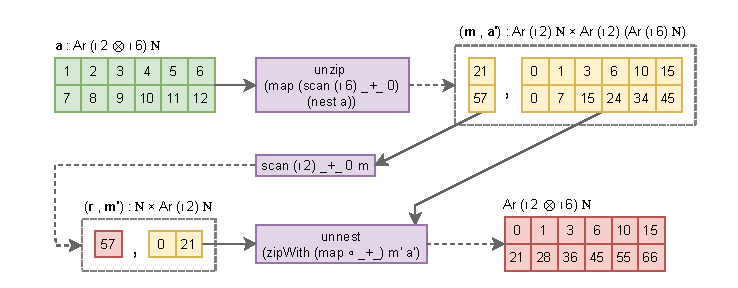
\includegraphics[width=\linewidth]{scan.drawio.pdf}
\Description{A data-flow diagram of scan with addition on a 2-by-6 array:
the rows are scanned, giving partial sums and scanned rows; the partial sums
are scanned, giving the overall sum and offsets that are added to the scanned
rows.}
\caption{\label{fig:scan}Application of rank-polymorphic \AF{scan} to 2-dimensional
array of natural numbers.}
\end{figure}
Colours distinguish arrays from operations.  The array \AB{a} (green, top-left)
of shape $(\AC{ι}\,2 \;\AC{⊗}\; \AC{ι}\,6)$ is the input.  It is fed to a
function (purple) that maps \texttt{scan} across the rows of \AB{a} and
\texttt{unzip}s the array of pairs into a pair of arrays.  Solid
arrows indicate inputs to functions; striped arrows indicate outputs.  The
result is a pair (shown in a dotted box, top-right) consisting of partial sums
(carries) and scanned rows.  We denote the projections of this pair by \AB{m}
and \AB{a'} respectively.  Both \AB{m} and \AB{a'} are coloured yellow,
signalling temporary data.  Scanning the partial sums \AB{m} produces a pair
containing the overall sum \AB{r} and a scan of the partial sums \AB{m'}.  The
overall sum \AB{r} is coloured red because it forms the first output of the
whole scan.  Finally, we adjust the rows of \AB{a'} by adding the corresponding
element from \AB{m'} to each row, \ie{} adding $0$ to the first row and $21$ to
the second row.  We transform the nested array into an array of product shape
using \texttt{unnest}.  This adjusted array constitutes the second output of the scan
and is likewise coloured red.


\subsection{Initial scan\label{sec:init-scan}}
%% agda: Stability
\begin{code}[hide]%
\>[0]\AgdaKeyword{module}\AgdaSpace{}%
\AgdaModule{IS}\AgdaSpace{}%
\AgdaKeyword{where}\<%
\\
\>[0][@{}l@{\AgdaIndent{0}}]%
\>[2]\AgdaKeyword{open}\AgdaSpace{}%
\AgdaModule{I}\<%
\\
%
\>[2]\AgdaKeyword{open}\AgdaSpace{}%
\AgdaModule{FromInit}\AgdaSpace{}%
\AgdaFunction{I.A}\<%
\\
%
\\[\AgdaEmptyExtraSkip]%
%
\>[2]\AgdaComment{--\ In\ the\ initial\ model,\ lifting\ shapes\ is\ the\ identity.\ \ We\ use\ this\ as\ a}\<%
\\
%
\>[2]\AgdaComment{--\ rewrite\ rule,\ so\ that\ initial\ scans\ apply\ directly\ to\ arrays\ of\ type\ I.Ar\ s\ X.}\<%
\\
%
\>[2]\AgdaFunction{⟦⟧s-id}\AgdaSpace{}%
\AgdaSymbol{:}\AgdaSpace{}%
\AgdaSymbol{∀}\AgdaSpace{}%
\AgdaSymbol{\{}\AgdaBound{s}\AgdaSpace{}%
\AgdaSymbol{:}\AgdaSpace{}%
\AgdaDatatype{I.S}\AgdaSymbol{\}}\AgdaSpace{}%
\AgdaSymbol{→}\AgdaSpace{}%
\AgdaOperator{\AgdaFunction{FromInit.⟦\AgdaUnderscore{}⟧s}}\AgdaSpace{}%
\AgdaFunction{I.A}\AgdaSpace{}%
\AgdaBound{s}\AgdaSpace{}%
\AgdaOperator{\AgdaDatatype{≡}}\AgdaSpace{}%
\AgdaBound{s}\<%
\\
%
\>[2]\AgdaFunction{⟦⟧s-id}\AgdaSpace{}%
\AgdaSymbol{\{}\AgdaInductiveConstructor{I.ι}\AgdaSpace{}%
\AgdaBound{n}\AgdaSymbol{\}}\AgdaSpace{}%
\AgdaSymbol{=}\AgdaSpace{}%
\AgdaInductiveConstructor{refl}\<%
\\
%
\>[2]\AgdaFunction{⟦⟧s-id}\AgdaSpace{}%
\AgdaSymbol{\{}\AgdaBound{s}\AgdaSpace{}%
\AgdaOperator{\AgdaInductiveConstructor{I.⊗}}\AgdaSpace{}%
\AgdaBound{p}\AgdaSymbol{\}}\AgdaSpace{}%
\AgdaSymbol{=}\AgdaSpace{}%
\AgdaFunction{cong₂}\AgdaSpace{}%
\AgdaOperator{\AgdaInductiveConstructor{I.\AgdaUnderscore{}⊗\AgdaUnderscore{}}}\AgdaSpace{}%
\AgdaFunction{⟦⟧s-id}\AgdaSpace{}%
\AgdaFunction{⟦⟧s-id}\<%
\\
%
\\[\AgdaEmptyExtraSkip]%
%
\\[\AgdaEmptyExtraSkip]%
%
\>[2]\AgdaKeyword{private}\AgdaSpace{}%
\AgdaKeyword{variable}\<%
\\
\>[2][@{}l@{\AgdaIndent{0}}]%
\>[4]\AgdaGeneralizable{X}\AgdaSpace{}%
\AgdaSymbol{:}\AgdaSpace{}%
\AgdaPrimitive{Set}\<%
\\
%
\>[4]\AgdaGeneralizable{s}\AgdaSpace{}%
\AgdaSymbol{:}\AgdaSpace{}%
\AgdaDatatype{S}\<%
\\
%
\>[4]\AgdaGeneralizable{n}\AgdaSpace{}%
\AgdaSymbol{:}\AgdaSpace{}%
\AgdaDatatype{ℕ}\<%
\\
%
\\[\AgdaEmptyExtraSkip]%
%
\>[2]\AgdaSymbol{\{-\#}\AgdaSpace{}%
\AgdaKeyword{REWRITE}\AgdaSpace{}%
\AgdaFunction{⟦⟧s-id}\AgdaSpace{}%
\AgdaSymbol{\#-\}}\<%
\\
%
\\[\AgdaEmptyExtraSkip]%
%
\>[2]\AgdaKeyword{open}\AgdaSpace{}%
\AgdaModule{Scan}\AgdaSpace{}%
\AgdaFunction{I.A}\AgdaSpace{}%
\AgdaSymbol{(}\AgdaFunction{CanonComb}\AgdaSpace{}%
\AgdaFunction{I.A}\AgdaSymbol{)}\AgdaSpace{}%
\AgdaSymbol{(}\AgdaFunction{CanonCombOk}\AgdaSpace{}%
\AgdaFunction{I.A}\AgdaSymbol{)}\AgdaSpace{}%
\AgdaKeyword{public}\<%
\\
\>[0]\<%
\\
%
\>[2]\AgdaFunction{scan₁-cong}%
\>[765I]\AgdaSymbol{:}\AgdaSpace{}%
\AgdaSymbol{∀}\AgdaSpace{}%
\AgdaSymbol{\{}\AgdaBound{s}\AgdaSymbol{\}}\AgdaSpace{}%
\AgdaSymbol{→}\AgdaSpace{}%
\AgdaSymbol{(}\AgdaBound{f}\AgdaSpace{}%
\AgdaSymbol{:}\AgdaSpace{}%
\AgdaGeneralizable{X}\AgdaSpace{}%
\AgdaSymbol{→}\AgdaSpace{}%
\AgdaGeneralizable{X}\AgdaSpace{}%
\AgdaSymbol{→}\AgdaSpace{}%
\AgdaGeneralizable{X}\AgdaSymbol{)}\AgdaSpace{}%
\AgdaSymbol{(}\AgdaBound{e}\AgdaSpace{}%
\AgdaSymbol{:}\AgdaSpace{}%
\AgdaGeneralizable{X}\AgdaSymbol{)}\AgdaSpace{}%
\AgdaSymbol{(}\AgdaBound{a}\AgdaSpace{}%
\AgdaBound{b}\AgdaSpace{}%
\AgdaSymbol{:}\AgdaSpace{}%
\AgdaFunction{Ar}\AgdaSpace{}%
\AgdaBound{s}\AgdaSpace{}%
\AgdaGeneralizable{X}\AgdaSymbol{)}\<%
\\
\>[.][@{}l@{}]\<[765I]%
\>[13]\AgdaSymbol{→}\AgdaSpace{}%
\AgdaBound{a}\AgdaSpace{}%
\AgdaOperator{\AgdaFunction{≈ₐ}}\AgdaSpace{}%
\AgdaBound{b}\AgdaSpace{}%
\AgdaSymbol{→}\AgdaSpace{}%
\AgdaFunction{scan₁}\AgdaSpace{}%
\AgdaBound{s}\AgdaSpace{}%
\AgdaBound{f}\AgdaSpace{}%
\AgdaBound{e}\AgdaSpace{}%
\AgdaBound{a}\AgdaSpace{}%
\AgdaOperator{\AgdaDatatype{≡}}\AgdaSpace{}%
\AgdaFunction{scan₁}\AgdaSpace{}%
\AgdaBound{s}\AgdaSpace{}%
\AgdaBound{f}\AgdaSpace{}%
\AgdaBound{e}\AgdaSpace{}%
\AgdaBound{b}\<%
\\
%
\\[\AgdaEmptyExtraSkip]%
%
\>[2]\AgdaFunction{scan₂-cong}%
\>[800I]\AgdaSymbol{:}\AgdaSpace{}%
\AgdaSymbol{∀}\AgdaSpace{}%
\AgdaSymbol{\{}\AgdaBound{s}\AgdaSymbol{\}}\AgdaSpace{}%
\AgdaSymbol{→}\AgdaSpace{}%
\AgdaSymbol{(}\AgdaBound{f}\AgdaSpace{}%
\AgdaSymbol{:}\AgdaSpace{}%
\AgdaGeneralizable{X}\AgdaSpace{}%
\AgdaSymbol{→}\AgdaSpace{}%
\AgdaGeneralizable{X}\AgdaSpace{}%
\AgdaSymbol{→}\AgdaSpace{}%
\AgdaGeneralizable{X}\AgdaSymbol{)}\AgdaSpace{}%
\AgdaSymbol{(}\AgdaBound{e}\AgdaSpace{}%
\AgdaSymbol{:}\AgdaSpace{}%
\AgdaGeneralizable{X}\AgdaSymbol{)}\AgdaSpace{}%
\AgdaSymbol{(}\AgdaBound{a}\AgdaSpace{}%
\AgdaBound{b}\AgdaSpace{}%
\AgdaSymbol{:}\AgdaSpace{}%
\AgdaFunction{Ar}\AgdaSpace{}%
\AgdaBound{s}\AgdaSpace{}%
\AgdaGeneralizable{X}\AgdaSymbol{)}\<%
\\
\>[.][@{}l@{}]\<[800I]%
\>[13]\AgdaSymbol{→}\AgdaSpace{}%
\AgdaBound{a}\AgdaSpace{}%
\AgdaOperator{\AgdaFunction{≈ₐ}}\AgdaSpace{}%
\AgdaBound{b}\AgdaSpace{}%
\AgdaSymbol{→}\AgdaSpace{}%
\AgdaFunction{scan₂}\AgdaSpace{}%
\AgdaBound{s}\AgdaSpace{}%
\AgdaBound{f}\AgdaSpace{}%
\AgdaBound{e}\AgdaSpace{}%
\AgdaBound{a}\AgdaSpace{}%
\AgdaOperator{\AgdaFunction{≈ₐ}}\AgdaSpace{}%
\AgdaFunction{scan₂}\AgdaSpace{}%
\AgdaBound{s}\AgdaSpace{}%
\AgdaBound{f}\AgdaSpace{}%
\AgdaBound{e}\AgdaSpace{}%
\AgdaBound{b}\<%
\\
\>[0]\<%
\\
%
\>[2]\AgdaComment{--\ Scans\ of\ initial\ vectors\ are\ congruent.}\<%
\\
%
\>[2]\AgdaFunction{scong₁}%
\>[835I]\AgdaSymbol{:}\AgdaSpace{}%
\AgdaSymbol{∀}\AgdaSpace{}%
\AgdaSymbol{\{}\AgdaBound{n}\AgdaSymbol{\}}\AgdaSpace{}%
\AgdaBound{f}\AgdaSpace{}%
\AgdaBound{e}\AgdaSpace{}%
\AgdaSymbol{(}\AgdaBound{a}\AgdaSpace{}%
\AgdaBound{b}\AgdaSpace{}%
\AgdaSymbol{:}\AgdaSpace{}%
\AgdaDatatype{I.P}\AgdaSpace{}%
\AgdaSymbol{(}\AgdaInductiveConstructor{I.ι}\AgdaSpace{}%
\AgdaBound{n}\AgdaSymbol{)}\AgdaSpace{}%
\AgdaSymbol{→}\AgdaSpace{}%
\AgdaGeneralizable{X}\AgdaSymbol{)}\AgdaSpace{}%
\AgdaSymbol{(}\AgdaBound{p}\AgdaSpace{}%
\AgdaSymbol{:}\AgdaSpace{}%
\AgdaSymbol{∀}\AgdaSpace{}%
\AgdaBound{i}\AgdaSpace{}%
\AgdaSymbol{→}\AgdaSpace{}%
\AgdaBound{a}\AgdaSpace{}%
\AgdaBound{i}\AgdaSpace{}%
\AgdaOperator{\AgdaDatatype{≡}}\AgdaSpace{}%
\AgdaBound{b}\AgdaSpace{}%
\AgdaBound{i}\AgdaSymbol{)}\<%
\\
\>[.][@{}l@{}]\<[835I]%
\>[9]\AgdaSymbol{→}\AgdaSpace{}%
\AgdaFunction{Vec.scan}\AgdaSpace{}%
\AgdaBound{f}\AgdaSpace{}%
\AgdaBound{e}\AgdaSpace{}%
\AgdaBound{a}\AgdaSpace{}%
\AgdaSymbol{.}\AgdaField{proj₁}\AgdaSpace{}%
\AgdaOperator{\AgdaDatatype{≡}}\AgdaSpace{}%
\AgdaFunction{Vec.scan}\AgdaSpace{}%
\AgdaBound{f}\AgdaSpace{}%
\AgdaBound{e}\AgdaSpace{}%
\AgdaBound{b}\AgdaSpace{}%
\AgdaSymbol{.}\AgdaField{proj₁}\<%
\\
%
\>[2]\AgdaFunction{scong₁}\AgdaSpace{}%
\AgdaSymbol{\{}\AgdaArgument{n}\AgdaSpace{}%
\AgdaSymbol{=}\AgdaSpace{}%
\AgdaInductiveConstructor{\#0}\AgdaSymbol{\}}\AgdaSpace{}%
\AgdaBound{f}\AgdaSpace{}%
\AgdaBound{e}\AgdaSpace{}%
\AgdaBound{a}\AgdaSpace{}%
\AgdaBound{b}\AgdaSpace{}%
\AgdaBound{p}\AgdaSpace{}%
\AgdaSymbol{=}\AgdaSpace{}%
\AgdaInductiveConstructor{refl}\<%
\\
%
\>[2]\AgdaFunction{scong₁}\AgdaSpace{}%
\AgdaSymbol{\{}\AgdaArgument{n}\AgdaSpace{}%
\AgdaSymbol{=}\AgdaSpace{}%
\AgdaInductiveConstructor{suc}\AgdaSpace{}%
\AgdaBound{n}\AgdaSymbol{\}}\AgdaSpace{}%
\AgdaBound{f}\AgdaSpace{}%
\AgdaBound{e}\AgdaSpace{}%
\AgdaBound{a}\AgdaSpace{}%
\AgdaBound{b}\AgdaSpace{}%
\AgdaBound{p}\AgdaSpace{}%
\AgdaSymbol{=}\<%
\\
\>[2][@{}l@{\AgdaIndent{0}}]%
\>[4]\AgdaFunction{scong₁}\AgdaSpace{}%
\AgdaBound{f}\AgdaSpace{}%
\AgdaSymbol{\AgdaUnderscore{}}\AgdaSpace{}%
\AgdaSymbol{(}\AgdaFunction{Vec.tl}\AgdaSpace{}%
\AgdaBound{a}\AgdaSymbol{)}\AgdaSpace{}%
\AgdaSymbol{(}\AgdaFunction{Vec.tl}\AgdaSpace{}%
\AgdaBound{b}\AgdaSymbol{)}\AgdaSpace{}%
\AgdaSymbol{(λ}\AgdaSpace{}%
\AgdaSymbol{\{}\AgdaSpace{}%
\AgdaSymbol{(}\AgdaInductiveConstructor{I.ι}\AgdaSpace{}%
\AgdaBound{i}\AgdaSymbol{)}\AgdaSpace{}%
\AgdaSymbol{→}\AgdaSpace{}%
\AgdaBound{p}\AgdaSpace{}%
\AgdaSymbol{(}\AgdaInductiveConstructor{I.ι}\AgdaSpace{}%
\AgdaOperator{\AgdaFunction{\$′}}\AgdaSpace{}%
\AgdaInductiveConstructor{suc}\AgdaSpace{}%
\AgdaBound{i}\AgdaSymbol{)}\AgdaSpace{}%
\AgdaSymbol{\})}\<%
\\
%
\>[4]\AgdaOperator{\AgdaFunction{⊡}}\AgdaSpace{}%
\AgdaFunction{cong}\AgdaSpace{}%
\AgdaSymbol{(λ}\AgdaSpace{}%
\AgdaBound{t}\AgdaSpace{}%
\AgdaSymbol{→}\AgdaSpace{}%
\AgdaFunction{Vec.scan}\AgdaSpace{}%
\AgdaBound{f}\AgdaSpace{}%
\AgdaBound{t}\AgdaSpace{}%
\AgdaSymbol{(}\AgdaFunction{Vec.tl}\AgdaSpace{}%
\AgdaBound{b}\AgdaSymbol{)}\AgdaSpace{}%
\AgdaSymbol{.}\AgdaField{proj₁}\AgdaSymbol{)}\AgdaSpace{}%
\AgdaSymbol{(}\AgdaFunction{cong}\AgdaSpace{}%
\AgdaSymbol{(}\AgdaBound{f}\AgdaSpace{}%
\AgdaBound{e}\AgdaSymbol{)}\AgdaSpace{}%
\AgdaSymbol{(}\AgdaBound{p}\AgdaSpace{}%
\AgdaSymbol{(}\AgdaInductiveConstructor{I.ι}\AgdaSpace{}%
\AgdaInductiveConstructor{\#0}\AgdaSymbol{)))}\<%
\\
%
\\[\AgdaEmptyExtraSkip]%
%
\>[2]\AgdaFunction{scong₂}%
\>[922I]\AgdaSymbol{:}\AgdaSpace{}%
\AgdaSymbol{∀}\AgdaSpace{}%
\AgdaSymbol{\{}\AgdaBound{n}\AgdaSymbol{\}}\AgdaSpace{}%
\AgdaBound{f}\AgdaSpace{}%
\AgdaBound{e}\AgdaSpace{}%
\AgdaSymbol{(}\AgdaBound{a}\AgdaSpace{}%
\AgdaBound{b}\AgdaSpace{}%
\AgdaSymbol{:}\AgdaSpace{}%
\AgdaDatatype{I.P}\AgdaSpace{}%
\AgdaSymbol{(}\AgdaInductiveConstructor{I.ι}\AgdaSpace{}%
\AgdaBound{n}\AgdaSymbol{)}\AgdaSpace{}%
\AgdaSymbol{→}\AgdaSpace{}%
\AgdaGeneralizable{X}\AgdaSymbol{)}\AgdaSpace{}%
\AgdaSymbol{(}\AgdaBound{p}\AgdaSpace{}%
\AgdaSymbol{:}\AgdaSpace{}%
\AgdaSymbol{∀}\AgdaSpace{}%
\AgdaBound{i}\AgdaSpace{}%
\AgdaSymbol{→}\AgdaSpace{}%
\AgdaBound{a}\AgdaSpace{}%
\AgdaBound{i}\AgdaSpace{}%
\AgdaOperator{\AgdaDatatype{≡}}\AgdaSpace{}%
\AgdaBound{b}\AgdaSpace{}%
\AgdaBound{i}\AgdaSymbol{)}\<%
\\
\>[.][@{}l@{}]\<[922I]%
\>[9]\AgdaSymbol{→}\AgdaSpace{}%
\AgdaSymbol{∀}\AgdaSpace{}%
\AgdaBound{i}\AgdaSpace{}%
\AgdaSymbol{→}\AgdaSpace{}%
\AgdaFunction{Vec.scan}\AgdaSpace{}%
\AgdaBound{f}\AgdaSpace{}%
\AgdaBound{e}\AgdaSpace{}%
\AgdaBound{a}\AgdaSpace{}%
\AgdaSymbol{.}\AgdaField{proj₂}\AgdaSpace{}%
\AgdaBound{i}\AgdaSpace{}%
\AgdaOperator{\AgdaDatatype{≡}}\AgdaSpace{}%
\AgdaFunction{Vec.scan}\AgdaSpace{}%
\AgdaBound{f}\AgdaSpace{}%
\AgdaBound{e}\AgdaSpace{}%
\AgdaBound{b}\AgdaSpace{}%
\AgdaSymbol{.}\AgdaField{proj₂}\AgdaSpace{}%
\AgdaBound{i}\<%
\\
%
\>[2]\AgdaFunction{scong₂}\AgdaSpace{}%
\AgdaSymbol{\{}\AgdaArgument{n}\AgdaSpace{}%
\AgdaSymbol{=}\AgdaSpace{}%
\AgdaInductiveConstructor{suc}\AgdaSpace{}%
\AgdaBound{n}\AgdaSymbol{\}}\AgdaSpace{}%
\AgdaBound{f}\AgdaSpace{}%
\AgdaBound{e}\AgdaSpace{}%
\AgdaBound{a}\AgdaSpace{}%
\AgdaBound{b}\AgdaSpace{}%
\AgdaBound{p}\AgdaSpace{}%
\AgdaSymbol{(}\AgdaInductiveConstructor{I.ι}\AgdaSpace{}%
\AgdaInductiveConstructor{\#0}\AgdaSymbol{)}\AgdaSpace{}%
\AgdaSymbol{=}\AgdaSpace{}%
\AgdaInductiveConstructor{refl}\<%
\\
%
\>[2]\AgdaFunction{scong₂}\AgdaSpace{}%
\AgdaSymbol{\{}\AgdaArgument{n}\AgdaSpace{}%
\AgdaSymbol{=}\AgdaSpace{}%
\AgdaInductiveConstructor{suc}\AgdaSpace{}%
\AgdaBound{n}\AgdaSymbol{\}}\AgdaSpace{}%
\AgdaBound{f}\AgdaSpace{}%
\AgdaBound{e}\AgdaSpace{}%
\AgdaBound{a}\AgdaSpace{}%
\AgdaBound{b}\AgdaSpace{}%
\AgdaBound{p}\AgdaSpace{}%
\AgdaSymbol{(}\AgdaInductiveConstructor{I.ι}\AgdaSpace{}%
\AgdaSymbol{(}\AgdaInductiveConstructor{suc}\AgdaSpace{}%
\AgdaBound{i}\AgdaSymbol{))}\AgdaSpace{}%
\AgdaSymbol{=}\<%
\\
\>[2][@{}l@{\AgdaIndent{0}}]%
\>[4]\AgdaFunction{scong₂}\AgdaSpace{}%
\AgdaBound{f}\AgdaSpace{}%
\AgdaSymbol{\AgdaUnderscore{}}\AgdaSpace{}%
\AgdaSymbol{(}\AgdaFunction{Vec.tl}\AgdaSpace{}%
\AgdaBound{a}\AgdaSymbol{)}\AgdaSpace{}%
\AgdaSymbol{(}\AgdaFunction{Vec.tl}\AgdaSpace{}%
\AgdaBound{b}\AgdaSymbol{)}\AgdaSpace{}%
\AgdaSymbol{(λ}\AgdaSpace{}%
\AgdaSymbol{\{}\AgdaSpace{}%
\AgdaSymbol{(}\AgdaInductiveConstructor{I.ι}\AgdaSpace{}%
\AgdaBound{j}\AgdaSymbol{)}\AgdaSpace{}%
\AgdaSymbol{→}\AgdaSpace{}%
\AgdaBound{p}\AgdaSpace{}%
\AgdaSymbol{(}\AgdaInductiveConstructor{I.ι}\AgdaSpace{}%
\AgdaOperator{\AgdaFunction{\$′}}\AgdaSpace{}%
\AgdaInductiveConstructor{suc}\AgdaSpace{}%
\AgdaBound{j}\AgdaSymbol{)}\AgdaSpace{}%
\AgdaSymbol{\})}\AgdaSpace{}%
\AgdaSymbol{(}\AgdaInductiveConstructor{I.ι}\AgdaSpace{}%
\AgdaBound{i}\AgdaSymbol{)}\<%
\\
%
\>[4]\AgdaOperator{\AgdaFunction{⊡}}\AgdaSpace{}%
\AgdaFunction{cong}\AgdaSpace{}%
\AgdaSymbol{(λ}\AgdaSpace{}%
\AgdaBound{t}\AgdaSpace{}%
\AgdaSymbol{→}\AgdaSpace{}%
\AgdaFunction{Vec.scan}\AgdaSpace{}%
\AgdaBound{f}\AgdaSpace{}%
\AgdaBound{t}\AgdaSpace{}%
\AgdaSymbol{(}\AgdaFunction{Vec.tl}\AgdaSpace{}%
\AgdaBound{b}\AgdaSymbol{)}\AgdaSpace{}%
\AgdaSymbol{.}\AgdaField{proj₂}\AgdaSpace{}%
\AgdaSymbol{(}\AgdaInductiveConstructor{I.ι}\AgdaSpace{}%
\AgdaBound{i}\AgdaSymbol{))}\AgdaSpace{}%
\AgdaSymbol{(}\AgdaFunction{cong}\AgdaSpace{}%
\AgdaSymbol{(}\AgdaBound{f}\AgdaSpace{}%
\AgdaBound{e}\AgdaSymbol{)}\AgdaSpace{}%
\AgdaSymbol{(}\AgdaBound{p}\AgdaSpace{}%
\AgdaSymbol{(}\AgdaInductiveConstructor{I.ι}\AgdaSpace{}%
\AgdaInductiveConstructor{\#0}\AgdaSymbol{)))}\<%
\\
%
\\[\AgdaEmptyExtraSkip]%
%
\>[2]\AgdaFunction{scan₁-cong}\AgdaSpace{}%
\AgdaSymbol{\{}\AgdaArgument{s}\AgdaSpace{}%
\AgdaSymbol{=}\AgdaSpace{}%
\AgdaInductiveConstructor{I.ι}\AgdaSpace{}%
\AgdaBound{n}\AgdaSymbol{\}}\AgdaSpace{}%
\AgdaBound{f}\AgdaSpace{}%
\AgdaBound{e}\AgdaSpace{}%
\AgdaBound{a}\AgdaSpace{}%
\AgdaBound{b}\AgdaSpace{}%
\AgdaBound{a≈b}\AgdaSpace{}%
\AgdaSymbol{=}\AgdaSpace{}%
\AgdaFunction{scong₁}\AgdaSpace{}%
\AgdaBound{f}\AgdaSpace{}%
\AgdaBound{e}\AgdaSpace{}%
\AgdaOperator{\AgdaFunction{⟦}}\AgdaSpace{}%
\AgdaBound{a}\AgdaSpace{}%
\AgdaOperator{\AgdaFunction{⟧a′}}\AgdaSpace{}%
\AgdaOperator{\AgdaFunction{⟦}}\AgdaSpace{}%
\AgdaBound{b}\AgdaSpace{}%
\AgdaOperator{\AgdaFunction{⟧a′}}\AgdaSpace{}%
\AgdaSymbol{(}\AgdaBound{a≈b}\AgdaSpace{}%
\AgdaOperator{\AgdaFunction{∘}}\AgdaSpace{}%
\AgdaOperator{\AgdaFunction{⟦\AgdaUnderscore{}⟧p}}\AgdaSymbol{)}\<%
\\
%
\>[2]\AgdaFunction{scan₁-cong}\AgdaSpace{}%
\AgdaSymbol{\{}\AgdaArgument{s}\AgdaSpace{}%
\AgdaSymbol{=}\AgdaSpace{}%
\AgdaBound{s}\AgdaSpace{}%
\AgdaOperator{\AgdaInductiveConstructor{I.⊗}}\AgdaSpace{}%
\AgdaBound{p}\AgdaSymbol{\}}\AgdaSpace{}%
\AgdaBound{f}\AgdaSpace{}%
\AgdaBound{e}\AgdaSpace{}%
\AgdaBound{a}\AgdaSpace{}%
\AgdaBound{b}\AgdaSpace{}%
\AgdaBound{a≈b}\<%
\\
\>[2][@{}l@{\AgdaIndent{0}}]%
\>[4]\AgdaSymbol{=}\AgdaSpace{}%
\AgdaFunction{scan₁-cong}\AgdaSpace{}%
\AgdaBound{f}\AgdaSpace{}%
\AgdaBound{e}\AgdaSpace{}%
\AgdaSymbol{\AgdaUnderscore{}}\AgdaSpace{}%
\AgdaSymbol{\AgdaUnderscore{}}\AgdaSpace{}%
\AgdaSymbol{(λ}\AgdaSpace{}%
\AgdaBound{i}\AgdaSpace{}%
\AgdaSymbol{→}\AgdaSpace{}%
\AgdaFunction{scan₁-cong}\AgdaSpace{}%
\AgdaBound{f}\AgdaSpace{}%
\AgdaBound{e}\AgdaSpace{}%
\AgdaSymbol{(}\AgdaBound{a}\AgdaSpace{}%
\AgdaOperator{\AgdaFunction{∘}}\AgdaSpace{}%
\AgdaSymbol{(}\AgdaBound{i}\AgdaSpace{}%
\AgdaOperator{\AgdaInductiveConstructor{⊗\AgdaUnderscore{}}}\AgdaSymbol{))}\AgdaSpace{}%
\AgdaSymbol{(}\AgdaBound{b}\AgdaSpace{}%
\AgdaOperator{\AgdaFunction{∘}}\AgdaSpace{}%
\AgdaSymbol{(}\AgdaBound{i}\AgdaSpace{}%
\AgdaOperator{\AgdaInductiveConstructor{⊗\AgdaUnderscore{}}}\AgdaSymbol{))}\AgdaSpace{}%
\AgdaSymbol{(}\AgdaBound{a≈b}\AgdaSpace{}%
\AgdaOperator{\AgdaFunction{∘}}\AgdaSpace{}%
\AgdaSymbol{(}\AgdaBound{i}\AgdaSpace{}%
\AgdaOperator{\AgdaInductiveConstructor{⊗\AgdaUnderscore{}}}\AgdaSymbol{)))}\<%
\\
%
\\[\AgdaEmptyExtraSkip]%
%
\>[2]\AgdaComment{--\ proof\ of\ scan₂-cong}\<%
\\
%
\>[2]\AgdaFunction{scan₂-cong}\AgdaSpace{}%
\AgdaSymbol{\{}\AgdaArgument{s}\AgdaSpace{}%
\AgdaSymbol{=}\AgdaSpace{}%
\AgdaInductiveConstructor{I.ι}\AgdaSpace{}%
\AgdaBound{n}\AgdaSymbol{\}}\AgdaSpace{}%
\AgdaBound{f}\AgdaSpace{}%
\AgdaBound{e}\AgdaSpace{}%
\AgdaBound{a}\AgdaSpace{}%
\AgdaBound{b}\AgdaSpace{}%
\AgdaBound{a≈b}\AgdaSpace{}%
\AgdaSymbol{(}\AgdaInductiveConstructor{I.ι}\AgdaSpace{}%
\AgdaBound{i}\AgdaSymbol{)}\<%
\\
\>[2][@{}l@{\AgdaIndent{0}}]%
\>[4]\AgdaSymbol{=}\AgdaSpace{}%
\AgdaFunction{scong₂}\AgdaSpace{}%
\AgdaBound{f}\AgdaSpace{}%
\AgdaBound{e}\AgdaSpace{}%
\AgdaSymbol{\AgdaUnderscore{}}\AgdaSpace{}%
\AgdaSymbol{\AgdaUnderscore{}}\AgdaSpace{}%
\AgdaSymbol{(}\AgdaBound{a≈b}\AgdaSpace{}%
\AgdaOperator{\AgdaFunction{∘}}\AgdaSpace{}%
\AgdaOperator{\AgdaFunction{⟦\AgdaUnderscore{}⟧p}}\AgdaSymbol{)}\AgdaSpace{}%
\AgdaSymbol{(}\AgdaInductiveConstructor{ι}\AgdaSpace{}%
\AgdaBound{i}\AgdaSymbol{)}\<%
\\
%
\\[\AgdaEmptyExtraSkip]%
%
\>[2]\AgdaFunction{scan₂-cong}\AgdaSpace{}%
\AgdaSymbol{\{}\AgdaArgument{s}\AgdaSpace{}%
\AgdaSymbol{=}\AgdaSpace{}%
\AgdaBound{s}\AgdaSpace{}%
\AgdaOperator{\AgdaInductiveConstructor{I.⊗}}\AgdaSpace{}%
\AgdaBound{p}\AgdaSymbol{\}}\AgdaSpace{}%
\AgdaBound{f}\AgdaSpace{}%
\AgdaBound{e}\AgdaSpace{}%
\AgdaBound{a}\AgdaSpace{}%
\AgdaBound{b}\AgdaSpace{}%
\AgdaBound{a≈b}\AgdaSpace{}%
\AgdaSymbol{(}\AgdaBound{i}\AgdaSpace{}%
\AgdaOperator{\AgdaInductiveConstructor{I.⊗}}\AgdaSpace{}%
\AgdaBound{j}\AgdaSymbol{)}\<%
\\
\>[2][@{}l@{\AgdaIndent{0}}]%
\>[4]\AgdaSymbol{=}%
\>[1113I]\AgdaFunction{cong₂}\AgdaSpace{}%
\AgdaBound{f}\<%
\\
\>[1113I][@{}l@{\AgdaIndent{0}}]%
\>[8]\AgdaSymbol{(}\AgdaFunction{scan₂-cong}\AgdaSpace{}%
\AgdaBound{f}\AgdaSpace{}%
\AgdaBound{e}\AgdaSpace{}%
\AgdaSymbol{\AgdaUnderscore{}}\AgdaSpace{}%
\AgdaSymbol{\AgdaUnderscore{}}\<%
\\
\>[8][@{}l@{\AgdaIndent{0}}]%
\>[11]\AgdaSymbol{(λ}\AgdaSpace{}%
\AgdaBound{ix}\AgdaSpace{}%
\AgdaSymbol{→}%
\>[1121I]\AgdaFunction{scan₁-cong}\AgdaSpace{}%
\AgdaBound{f}\AgdaSpace{}%
\AgdaBound{e}\<%
\\
\>[1121I][@{}l@{\AgdaIndent{0}}]%
\>[23]\AgdaSymbol{(}\AgdaBound{a}\AgdaSpace{}%
\AgdaOperator{\AgdaFunction{∘}}\AgdaSpace{}%
\AgdaSymbol{(}\AgdaBound{ix}\AgdaSpace{}%
\AgdaOperator{\AgdaInductiveConstructor{⊗\AgdaUnderscore{}}}\AgdaSymbol{))}\<%
\\
%
\>[23]\AgdaSymbol{(}\AgdaBound{b}\AgdaSpace{}%
\AgdaOperator{\AgdaFunction{∘}}\AgdaSpace{}%
\AgdaSymbol{(}\AgdaBound{ix}\AgdaSpace{}%
\AgdaOperator{\AgdaInductiveConstructor{⊗\AgdaUnderscore{}}}\AgdaSymbol{))}\<%
\\
%
\>[23]\AgdaSymbol{(λ}\AgdaSpace{}%
\AgdaBound{k}\AgdaSpace{}%
\AgdaSymbol{→}\AgdaSpace{}%
\AgdaBound{a≈b}\AgdaSpace{}%
\AgdaSymbol{(}\AgdaBound{ix}\AgdaSpace{}%
\AgdaOperator{\AgdaInductiveConstructor{⊗}}\AgdaSpace{}%
\AgdaBound{k}\AgdaSymbol{)))}\AgdaSpace{}%
\AgdaBound{i}\AgdaSymbol{)}\<%
\\
%
\>[8]\AgdaSymbol{(}\AgdaFunction{scan₂-cong}\AgdaSpace{}%
\AgdaBound{f}\AgdaSpace{}%
\AgdaBound{e}\AgdaSpace{}%
\AgdaSymbol{(}\AgdaBound{a}\AgdaSpace{}%
\AgdaOperator{\AgdaFunction{∘}}\AgdaSpace{}%
\AgdaSymbol{(}\AgdaBound{i}\AgdaSpace{}%
\AgdaOperator{\AgdaInductiveConstructor{⊗\AgdaUnderscore{}}}\AgdaSymbol{))}\AgdaSpace{}%
\AgdaSymbol{(}\AgdaBound{b}\AgdaSpace{}%
\AgdaOperator{\AgdaFunction{∘}}\AgdaSpace{}%
\AgdaSymbol{(}\AgdaBound{i}\AgdaSpace{}%
\AgdaOperator{\AgdaInductiveConstructor{⊗\AgdaUnderscore{}}}\AgdaSymbol{))}\AgdaSpace{}%
\AgdaSymbol{(}\AgdaBound{a≈b}\AgdaSpace{}%
\AgdaOperator{\AgdaFunction{∘}}\AgdaSpace{}%
\AgdaSymbol{(}\AgdaBound{i}\AgdaSpace{}%
\AgdaOperator{\AgdaInductiveConstructor{⊗\AgdaUnderscore{}}}\AgdaSymbol{))}\AgdaSpace{}%
\AgdaBound{j}\AgdaSymbol{)}\<%
\end{code}  
As \texttt{scan} is defined for all models, it can be instantiated for the
initial model with the canonical combinators:
\begin{mathpar}
\AK{module}\ \AM{IS}\ =\ \AM{Scan}\ \AF{I.A}\ (\AF{CanonComb}\ \AF{I.A})\
     (\AF{CanonCombOk}\ \AF{I.A})
\end{mathpar}

This instance of \texttt{scan} is noteworthy because we can prove that, for any
array model \AB{A} and for any semantically-respecting combinators, the results
computed by \texttt{scan} for that model coincide with those computed by the
initial scan.  Formally:
\begin{mathpar}\codeblock{\begin{code}[hide]%
\>[0]\AgdaKeyword{module}\AgdaSpace{}%
\AgdaModule{ScanOk}\AgdaSpace{}%
\AgdaSymbol{(}\AgdaBound{A}\AgdaSpace{}%
\AgdaSymbol{:}\AgdaSpace{}%
\AgdaRecord{Array}\AgdaSymbol{)}\AgdaSpace{}%
\AgdaSymbol{(}\AgdaBound{Native}\AgdaSpace{}%
\AgdaSymbol{:}\AgdaSpace{}%
\AgdaRecord{Comb}\AgdaSpace{}%
\AgdaBound{A}\AgdaSymbol{)}\AgdaSpace{}%
\AgdaSymbol{(}\AgdaBound{Ok}\AgdaSpace{}%
\AgdaSymbol{:}\AgdaSpace{}%
\AgdaRecord{CombOk}\AgdaSpace{}%
\AgdaBound{A}\AgdaSpace{}%
\AgdaBound{Native}\AgdaSymbol{)}\AgdaSpace{}%
\AgdaKeyword{where}\<%
\\
\>[0][@{}l@{\AgdaIndent{0}}]%
\>[2]\AgdaKeyword{open}\AgdaSpace{}%
\AgdaModule{Array}\AgdaSpace{}%
\AgdaBound{A}\<%
\\
%
\>[2]\AgdaKeyword{open}\AgdaSpace{}%
\AgdaModule{ArOps}\AgdaSpace{}%
\AgdaBound{A}\<%
\\
%
\>[2]\AgdaKeyword{open}\AgdaSpace{}%
\AgdaModule{Comb}\AgdaSpace{}%
\AgdaBound{Native}\<%
\\
%
\>[2]\AgdaKeyword{open}\AgdaSpace{}%
\AgdaModule{CombOk}\AgdaSpace{}%
\AgdaBound{Ok}\<%
\\
%
\>[2]\AgdaKeyword{open}\AgdaSpace{}%
\AgdaModule{FromInit}\AgdaSpace{}%
\AgdaBound{A}\<%
\\
%
\>[2]\AgdaKeyword{open}\AgdaSpace{}%
\AgdaModule{Scan}\AgdaSpace{}%
\AgdaBound{A}\AgdaSpace{}%
\AgdaBound{Native}\AgdaSpace{}%
\AgdaBound{Ok}\<%
\\
%
\\[\AgdaEmptyExtraSkip]%
%
\>[2]\AgdaKeyword{private}\AgdaSpace{}%
\AgdaKeyword{variable}\<%
\\
\>[2][@{}l@{\AgdaIndent{0}}]%
\>[4]\AgdaGeneralizable{X}\AgdaSpace{}%
\AgdaGeneralizable{Y}\AgdaSpace{}%
\AgdaGeneralizable{Z}\AgdaSpace{}%
\AgdaSymbol{:}\AgdaSpace{}%
\AgdaPrimitive{Set}\<%
\\
%
\>[4]\AgdaGeneralizable{s}\AgdaSpace{}%
\AgdaGeneralizable{p}\AgdaSpace{}%
\AgdaSymbol{:}\AgdaSpace{}%
\AgdaFunction{S}\<%
\\
\>[0]\<%
\end{code}
\begin{code}%
\>[0][@{}l@{\AgdaIndent{1}}]%
\>[2]\AgdaFunction{scan-ok}%
\>[1188I]\AgdaSymbol{:}\AgdaSpace{}%
\AgdaSymbol{(}\AgdaBound{s}\AgdaSpace{}%
\AgdaSymbol{:}\AgdaSpace{}%
\AgdaDatatype{I.S}\AgdaSymbol{)}\AgdaSpace{}%
\AgdaSymbol{→}\AgdaSpace{}%
\AgdaSymbol{(}\AgdaBound{f}\AgdaSpace{}%
\AgdaSymbol{:}\AgdaSpace{}%
\AgdaGeneralizable{X}\AgdaSpace{}%
\AgdaSymbol{→}\AgdaSpace{}%
\AgdaGeneralizable{X}\AgdaSpace{}%
\AgdaSymbol{→}\AgdaSpace{}%
\AgdaGeneralizable{X}\AgdaSymbol{)}\AgdaSpace{}%
\AgdaSymbol{→}\AgdaSpace{}%
\AgdaSymbol{(}\AgdaBound{e}\AgdaSpace{}%
\AgdaSymbol{:}\AgdaSpace{}%
\AgdaGeneralizable{X}\AgdaSymbol{)}\AgdaSpace{}%
\AgdaSymbol{→}\AgdaSpace{}%
\AgdaSymbol{(}\AgdaBound{a}\AgdaSpace{}%
\AgdaSymbol{:}\AgdaSpace{}%
\AgdaFunction{Ar}\AgdaSpace{}%
\AgdaOperator{\AgdaFunction{⟦}}\AgdaSpace{}%
\AgdaBound{s}\AgdaSpace{}%
\AgdaOperator{\AgdaFunction{⟧s}}\AgdaSpace{}%
\AgdaGeneralizable{X}\AgdaSymbol{)}\<%
\\
\>[.][@{}l@{}]\<[1188I]%
\>[10]\AgdaSymbol{→}%
\>[13]\AgdaFunction{scan₁}\AgdaSpace{}%
\AgdaBound{s}\AgdaSpace{}%
\AgdaBound{f}\AgdaSpace{}%
\AgdaBound{e}\AgdaSpace{}%
\AgdaBound{a}%
\>[29]\AgdaOperator{\AgdaDatatype{≡}}%
\>[33]\AgdaFunction{IS.scan₁}\AgdaSpace{}%
\AgdaBound{s}\AgdaSpace{}%
\AgdaBound{f}\AgdaSpace{}%
\AgdaBound{e}\AgdaSpace{}%
\AgdaOperator{\AgdaFunction{⟦}}\AgdaSpace{}%
\AgdaBound{a}\AgdaSpace{}%
\AgdaOperator{\AgdaFunction{⟧a′}}\<%
\\
%
\>[10]\AgdaOperator{\AgdaFunction{×}}%
\>[13]\AgdaFunction{scan₂}\AgdaSpace{}%
\AgdaBound{s}\AgdaSpace{}%
\AgdaBound{f}\AgdaSpace{}%
\AgdaBound{e}\AgdaSpace{}%
\AgdaBound{a}%
\>[29]\AgdaOperator{\AgdaFunction{≈ₐ}}%
\>[33]\AgdaOperator{\AgdaFunction{⟦}}\AgdaSpace{}%
\AgdaFunction{IS.scan₂}\AgdaSpace{}%
\AgdaBound{s}\AgdaSpace{}%
\AgdaBound{f}\AgdaSpace{}%
\AgdaBound{e}\AgdaSpace{}%
\AgdaOperator{\AgdaFunction{⟦}}\AgdaSpace{}%
\AgdaBound{a}\AgdaSpace{}%
\AgdaOperator{\AgdaFunction{⟧a′}}\AgdaSpace{}%
\AgdaOperator{\AgdaFunction{⟧a}}\<%
\end{code}}
\end{mathpar}
In essence, the theorem states that all scans in all models compute the same
values: whenever two models \AB{A} and \AB{B} share the same (lifted) shape and
the same element values, their respective scans produce identical results.  We
prove the theorem by induction on the shape $s$, using the fact that the
combinators respect their intended semantics (\AB{Ok}) to show that the
translation artefacts introduced by moving between models do not affect the
computed values.  The theorem would also follow from the
parametricity~\citep{reynolds1983types} of \texttt{scan} over array models
together with the initiality of the initial model.  However, Agda does not
internalise parametricity, so using this argument would require defining an
embedded language, re-expressing the array theory and combinators within it,
and proving a general parametricity result \`a la
\citet{10.1145/1863543.1863592}.  The direct proof is considerably simpler.

\begin{code}[hide]%
%
\>[2]\AgdaComment{--\ Selecting\ from\ the\ results\ of\ native\ combinators,\ derived\ from\ CombOk.}\<%
\\
%
\>[2]\AgdaFunction{map-sel}\AgdaSpace{}%
\AgdaSymbol{:}\AgdaSpace{}%
\AgdaSymbol{(}\AgdaBound{g}\AgdaSpace{}%
\AgdaSymbol{:}\AgdaSpace{}%
\AgdaGeneralizable{X}\AgdaSpace{}%
\AgdaSymbol{→}\AgdaSpace{}%
\AgdaGeneralizable{Y}\AgdaSymbol{)}\AgdaSpace{}%
\AgdaSymbol{(}\AgdaBound{a}\AgdaSpace{}%
\AgdaSymbol{:}\AgdaSpace{}%
\AgdaFunction{Ar}\AgdaSpace{}%
\AgdaGeneralizable{s}\AgdaSpace{}%
\AgdaGeneralizable{X}\AgdaSymbol{)}\AgdaSpace{}%
\AgdaSymbol{(}\AgdaBound{i}\AgdaSpace{}%
\AgdaSymbol{:}\AgdaSpace{}%
\AgdaFunction{P}\AgdaSpace{}%
\AgdaGeneralizable{s}\AgdaSymbol{)}\AgdaSpace{}%
\AgdaSymbol{→}\AgdaSpace{}%
\AgdaFunction{map}\AgdaSpace{}%
\AgdaBound{g}\AgdaSpace{}%
\AgdaBound{a}\AgdaSpace{}%
\AgdaOperator{\AgdaFunction{[}}\AgdaSpace{}%
\AgdaBound{i}\AgdaSpace{}%
\AgdaOperator{\AgdaFunction{]}}\AgdaSpace{}%
\AgdaOperator{\AgdaDatatype{≡}}\AgdaSpace{}%
\AgdaBound{g}\AgdaSpace{}%
\AgdaSymbol{(}\AgdaBound{a}\AgdaSpace{}%
\AgdaOperator{\AgdaFunction{[}}\AgdaSpace{}%
\AgdaBound{i}\AgdaSpace{}%
\AgdaOperator{\AgdaFunction{]}}\AgdaSymbol{)}\<%
\\
%
\>[2]\AgdaFunction{map-sel}\AgdaSpace{}%
\AgdaBound{g}\AgdaSpace{}%
\AgdaBound{a}\AgdaSpace{}%
\AgdaBound{i}\AgdaSpace{}%
\AgdaSymbol{=}\AgdaSpace{}%
\AgdaField{map-ok}\AgdaSpace{}%
\AgdaBound{g}\AgdaSpace{}%
\AgdaBound{a}\AgdaSpace{}%
\AgdaBound{i}\AgdaSpace{}%
\AgdaOperator{\AgdaFunction{⊡}}\AgdaSpace{}%
\AgdaFunction{sel-imap}\AgdaSpace{}%
\AgdaSymbol{\AgdaUnderscore{}}\AgdaSpace{}%
\AgdaBound{i}\<%
\\
%
\\[\AgdaEmptyExtraSkip]%
%
\>[2]\AgdaFunction{nest-sel}\AgdaSpace{}%
\AgdaSymbol{:}\AgdaSpace{}%
\AgdaSymbol{(}\AgdaBound{a}\AgdaSpace{}%
\AgdaSymbol{:}\AgdaSpace{}%
\AgdaFunction{Ar}\AgdaSpace{}%
\AgdaSymbol{(}\AgdaGeneralizable{s}\AgdaSpace{}%
\AgdaOperator{\AgdaFunction{⊗}}\AgdaSpace{}%
\AgdaGeneralizable{p}\AgdaSymbol{)}\AgdaSpace{}%
\AgdaGeneralizable{X}\AgdaSymbol{)}\AgdaSpace{}%
\AgdaSymbol{(}\AgdaBound{i}\AgdaSpace{}%
\AgdaSymbol{:}\AgdaSpace{}%
\AgdaFunction{P}\AgdaSpace{}%
\AgdaGeneralizable{s}\AgdaSymbol{)}\AgdaSpace{}%
\AgdaSymbol{(}\AgdaBound{j}\AgdaSpace{}%
\AgdaSymbol{:}\AgdaSpace{}%
\AgdaFunction{P}\AgdaSpace{}%
\AgdaGeneralizable{p}\AgdaSymbol{)}\AgdaSpace{}%
\AgdaSymbol{→}\AgdaSpace{}%
\AgdaFunction{nest}\AgdaSpace{}%
\AgdaBound{a}\AgdaSpace{}%
\AgdaOperator{\AgdaFunction{[}}\AgdaSpace{}%
\AgdaBound{i}\AgdaSpace{}%
\AgdaOperator{\AgdaFunction{]}}\AgdaSpace{}%
\AgdaOperator{\AgdaFunction{[}}\AgdaSpace{}%
\AgdaBound{j}\AgdaSpace{}%
\AgdaOperator{\AgdaFunction{]}}\AgdaSpace{}%
\AgdaOperator{\AgdaDatatype{≡}}\AgdaSpace{}%
\AgdaBound{a}\AgdaSpace{}%
\AgdaOperator{\AgdaFunction{[}}\AgdaSpace{}%
\AgdaBound{i}\AgdaSpace{}%
\AgdaOperator{\AgdaFunction{⊛}}\AgdaSpace{}%
\AgdaBound{j}\AgdaSpace{}%
\AgdaOperator{\AgdaFunction{]}}\<%
\\
%
\>[2]\AgdaFunction{nest-sel}\AgdaSpace{}%
\AgdaBound{a}\AgdaSpace{}%
\AgdaBound{i}\AgdaSpace{}%
\AgdaBound{j}\AgdaSpace{}%
\AgdaSymbol{=}\AgdaSpace{}%
\AgdaFunction{cong}\AgdaSpace{}%
\AgdaSymbol{(}\AgdaOperator{\AgdaFunction{\AgdaUnderscore{}[}}\AgdaSpace{}%
\AgdaBound{j}\AgdaSpace{}%
\AgdaOperator{\AgdaFunction{]}}\AgdaSymbol{)}\AgdaSpace{}%
\AgdaSymbol{(}\AgdaField{nest-ok}\AgdaSpace{}%
\AgdaBound{a}\AgdaSpace{}%
\AgdaBound{i}\AgdaSpace{}%
\AgdaOperator{\AgdaFunction{⊡}}\AgdaSpace{}%
\AgdaFunction{sel-imap}\AgdaSpace{}%
\AgdaSymbol{\AgdaUnderscore{}}\AgdaSpace{}%
\AgdaBound{i}\AgdaSymbol{)}\AgdaSpace{}%
\AgdaOperator{\AgdaFunction{⊡}}\AgdaSpace{}%
\AgdaFunction{sel-imap}\AgdaSpace{}%
\AgdaSymbol{\AgdaUnderscore{}}\AgdaSpace{}%
\AgdaBound{j}\<%
\\
%
\\[\AgdaEmptyExtraSkip]%
%
\>[2]\AgdaFunction{unnest-sel}\AgdaSpace{}%
\AgdaSymbol{:}\AgdaSpace{}%
\AgdaSymbol{(}\AgdaBound{a}\AgdaSpace{}%
\AgdaSymbol{:}\AgdaSpace{}%
\AgdaFunction{Ar}\AgdaSpace{}%
\AgdaGeneralizable{s}\AgdaSpace{}%
\AgdaSymbol{(}\AgdaFunction{Ar}\AgdaSpace{}%
\AgdaGeneralizable{p}\AgdaSpace{}%
\AgdaGeneralizable{X}\AgdaSymbol{))}\AgdaSpace{}%
\AgdaSymbol{(}\AgdaBound{i}\AgdaSpace{}%
\AgdaSymbol{:}\AgdaSpace{}%
\AgdaFunction{P}\AgdaSpace{}%
\AgdaSymbol{(}\AgdaGeneralizable{s}\AgdaSpace{}%
\AgdaOperator{\AgdaFunction{⊗}}\AgdaSpace{}%
\AgdaGeneralizable{p}\AgdaSymbol{))}\AgdaSpace{}%
\AgdaSymbol{→}\AgdaSpace{}%
\AgdaFunction{unnest}\AgdaSpace{}%
\AgdaBound{a}\AgdaSpace{}%
\AgdaOperator{\AgdaFunction{[}}\AgdaSpace{}%
\AgdaBound{i}\AgdaSpace{}%
\AgdaOperator{\AgdaFunction{]}}\AgdaSpace{}%
\AgdaOperator{\AgdaDatatype{≡}}\AgdaSpace{}%
\AgdaBound{a}\AgdaSpace{}%
\AgdaOperator{\AgdaFunction{[}}\AgdaSpace{}%
\AgdaFunction{fst}\AgdaSpace{}%
\AgdaBound{i}\AgdaSpace{}%
\AgdaOperator{\AgdaFunction{]}}\AgdaSpace{}%
\AgdaOperator{\AgdaFunction{[}}\AgdaSpace{}%
\AgdaFunction{snd}\AgdaSpace{}%
\AgdaBound{i}\AgdaSpace{}%
\AgdaOperator{\AgdaFunction{]}}\<%
\\
%
\>[2]\AgdaFunction{unnest-sel}\AgdaSpace{}%
\AgdaBound{a}\AgdaSpace{}%
\AgdaBound{i}\AgdaSpace{}%
\AgdaSymbol{=}\AgdaSpace{}%
\AgdaField{unnest-ok}\AgdaSpace{}%
\AgdaBound{a}\AgdaSpace{}%
\AgdaBound{i}\AgdaSpace{}%
\AgdaOperator{\AgdaFunction{⊡}}\AgdaSpace{}%
\AgdaFunction{sel-imap}\AgdaSpace{}%
\AgdaSymbol{\AgdaUnderscore{}}\AgdaSpace{}%
\AgdaBound{i}\<%
\\
%
\\[\AgdaEmptyExtraSkip]%
%
\>[2]\AgdaFunction{zipWith-sel}%
\>[1365I]\AgdaSymbol{:}\AgdaSpace{}%
\AgdaSymbol{(}\AgdaBound{g}\AgdaSpace{}%
\AgdaSymbol{:}\AgdaSpace{}%
\AgdaGeneralizable{X}\AgdaSpace{}%
\AgdaSymbol{→}\AgdaSpace{}%
\AgdaGeneralizable{Y}\AgdaSpace{}%
\AgdaSymbol{→}\AgdaSpace{}%
\AgdaGeneralizable{Z}\AgdaSymbol{)}\AgdaSpace{}%
\AgdaSymbol{(}\AgdaBound{a}\AgdaSpace{}%
\AgdaSymbol{:}\AgdaSpace{}%
\AgdaFunction{Ar}\AgdaSpace{}%
\AgdaGeneralizable{s}\AgdaSpace{}%
\AgdaGeneralizable{X}\AgdaSymbol{)}\AgdaSpace{}%
\AgdaSymbol{(}\AgdaBound{b}\AgdaSpace{}%
\AgdaSymbol{:}\AgdaSpace{}%
\AgdaFunction{Ar}\AgdaSpace{}%
\AgdaGeneralizable{s}\AgdaSpace{}%
\AgdaGeneralizable{Y}\AgdaSymbol{)}\AgdaSpace{}%
\AgdaSymbol{(}\AgdaBound{i}\AgdaSpace{}%
\AgdaSymbol{:}\AgdaSpace{}%
\AgdaFunction{P}\AgdaSpace{}%
\AgdaGeneralizable{s}\AgdaSymbol{)}\<%
\\
\>[.][@{}l@{}]\<[1365I]%
\>[14]\AgdaSymbol{→}\AgdaSpace{}%
\AgdaFunction{zipWith}\AgdaSpace{}%
\AgdaBound{g}\AgdaSpace{}%
\AgdaBound{a}\AgdaSpace{}%
\AgdaBound{b}\AgdaSpace{}%
\AgdaOperator{\AgdaFunction{[}}\AgdaSpace{}%
\AgdaBound{i}\AgdaSpace{}%
\AgdaOperator{\AgdaFunction{]}}\AgdaSpace{}%
\AgdaOperator{\AgdaDatatype{≡}}\AgdaSpace{}%
\AgdaBound{g}\AgdaSpace{}%
\AgdaSymbol{(}\AgdaBound{a}\AgdaSpace{}%
\AgdaOperator{\AgdaFunction{[}}\AgdaSpace{}%
\AgdaBound{i}\AgdaSpace{}%
\AgdaOperator{\AgdaFunction{]}}\AgdaSymbol{)}\AgdaSpace{}%
\AgdaSymbol{(}\AgdaBound{b}\AgdaSpace{}%
\AgdaOperator{\AgdaFunction{[}}\AgdaSpace{}%
\AgdaBound{i}\AgdaSpace{}%
\AgdaOperator{\AgdaFunction{]}}\AgdaSymbol{)}\<%
\\
%
\>[2]\AgdaFunction{zipWith-sel}\AgdaSpace{}%
\AgdaBound{g}\AgdaSpace{}%
\AgdaBound{a}\AgdaSpace{}%
\AgdaBound{b}\AgdaSpace{}%
\AgdaBound{i}\AgdaSpace{}%
\AgdaSymbol{=}\AgdaSpace{}%
\AgdaField{zipWith-ok}\AgdaSpace{}%
\AgdaBound{g}\AgdaSpace{}%
\AgdaBound{a}\AgdaSpace{}%
\AgdaBound{b}\AgdaSpace{}%
\AgdaBound{i}\AgdaSpace{}%
\AgdaOperator{\AgdaFunction{⊡}}\AgdaSpace{}%
\AgdaFunction{sel-imap}\AgdaSpace{}%
\AgdaSymbol{\AgdaUnderscore{}}\AgdaSpace{}%
\AgdaBound{i}\<%
\\
%
\\[\AgdaEmptyExtraSkip]%
%
\>[2]\AgdaFunction{unzip₁-sel}\AgdaSpace{}%
\AgdaSymbol{:}\AgdaSpace{}%
\AgdaSymbol{(}\AgdaBound{a}\AgdaSpace{}%
\AgdaSymbol{:}\AgdaSpace{}%
\AgdaFunction{Ar}\AgdaSpace{}%
\AgdaGeneralizable{s}\AgdaSpace{}%
\AgdaSymbol{(}\AgdaGeneralizable{X}\AgdaSpace{}%
\AgdaOperator{\AgdaFunction{×}}\AgdaSpace{}%
\AgdaGeneralizable{Y}\AgdaSymbol{))}\AgdaSpace{}%
\AgdaSymbol{(}\AgdaBound{i}\AgdaSpace{}%
\AgdaSymbol{:}\AgdaSpace{}%
\AgdaFunction{P}\AgdaSpace{}%
\AgdaGeneralizable{s}\AgdaSymbol{)}\AgdaSpace{}%
\AgdaSymbol{→}\AgdaSpace{}%
\AgdaField{proj₁}\AgdaSpace{}%
\AgdaSymbol{(}\AgdaFunction{unzip}\AgdaSpace{}%
\AgdaBound{a}\AgdaSymbol{)}\AgdaSpace{}%
\AgdaOperator{\AgdaFunction{[}}\AgdaSpace{}%
\AgdaBound{i}\AgdaSpace{}%
\AgdaOperator{\AgdaFunction{]}}\AgdaSpace{}%
\AgdaOperator{\AgdaDatatype{≡}}\AgdaSpace{}%
\AgdaField{proj₁}\AgdaSpace{}%
\AgdaSymbol{(}\AgdaBound{a}\AgdaSpace{}%
\AgdaOperator{\AgdaFunction{[}}\AgdaSpace{}%
\AgdaBound{i}\AgdaSpace{}%
\AgdaOperator{\AgdaFunction{]}}\AgdaSymbol{)}\<%
\\
%
\>[2]\AgdaFunction{unzip₁-sel}\AgdaSpace{}%
\AgdaBound{a}\AgdaSpace{}%
\AgdaBound{i}\AgdaSpace{}%
\AgdaSymbol{=}\AgdaSpace{}%
\AgdaField{unzip-ok}\AgdaSpace{}%
\AgdaBound{a}\AgdaSpace{}%
\AgdaSymbol{.}\AgdaField{proj₁}\AgdaSpace{}%
\AgdaBound{i}\AgdaSpace{}%
\AgdaOperator{\AgdaFunction{⊡}}\AgdaSpace{}%
\AgdaFunction{sel-imap}\AgdaSpace{}%
\AgdaSymbol{\AgdaUnderscore{}}\AgdaSpace{}%
\AgdaBound{i}\<%
\\
%
\\[\AgdaEmptyExtraSkip]%
%
\>[2]\AgdaFunction{unzip₂-sel}\AgdaSpace{}%
\AgdaSymbol{:}\AgdaSpace{}%
\AgdaSymbol{(}\AgdaBound{a}\AgdaSpace{}%
\AgdaSymbol{:}\AgdaSpace{}%
\AgdaFunction{Ar}\AgdaSpace{}%
\AgdaGeneralizable{s}\AgdaSpace{}%
\AgdaSymbol{(}\AgdaGeneralizable{X}\AgdaSpace{}%
\AgdaOperator{\AgdaFunction{×}}\AgdaSpace{}%
\AgdaGeneralizable{Y}\AgdaSymbol{))}\AgdaSpace{}%
\AgdaSymbol{(}\AgdaBound{i}\AgdaSpace{}%
\AgdaSymbol{:}\AgdaSpace{}%
\AgdaFunction{P}\AgdaSpace{}%
\AgdaGeneralizable{s}\AgdaSymbol{)}\AgdaSpace{}%
\AgdaSymbol{→}\AgdaSpace{}%
\AgdaField{proj₂}\AgdaSpace{}%
\AgdaSymbol{(}\AgdaFunction{unzip}\AgdaSpace{}%
\AgdaBound{a}\AgdaSymbol{)}\AgdaSpace{}%
\AgdaOperator{\AgdaFunction{[}}\AgdaSpace{}%
\AgdaBound{i}\AgdaSpace{}%
\AgdaOperator{\AgdaFunction{]}}\AgdaSpace{}%
\AgdaOperator{\AgdaDatatype{≡}}\AgdaSpace{}%
\AgdaField{proj₂}\AgdaSpace{}%
\AgdaSymbol{(}\AgdaBound{a}\AgdaSpace{}%
\AgdaOperator{\AgdaFunction{[}}\AgdaSpace{}%
\AgdaBound{i}\AgdaSpace{}%
\AgdaOperator{\AgdaFunction{]}}\AgdaSymbol{)}\<%
\\
%
\>[2]\AgdaFunction{unzip₂-sel}\AgdaSpace{}%
\AgdaBound{a}\AgdaSpace{}%
\AgdaBound{i}\AgdaSpace{}%
\AgdaSymbol{=}\AgdaSpace{}%
\AgdaField{unzip-ok}\AgdaSpace{}%
\AgdaBound{a}\AgdaSpace{}%
\AgdaSymbol{.}\AgdaField{proj₂}\AgdaSpace{}%
\AgdaBound{i}\AgdaSpace{}%
\AgdaOperator{\AgdaFunction{⊡}}\AgdaSpace{}%
\AgdaFunction{sel-imap}\AgdaSpace{}%
\AgdaSymbol{\AgdaUnderscore{}}\AgdaSpace{}%
\AgdaBound{i}\<%
\\
%
\\[\AgdaEmptyExtraSkip]%
%
\>[2]\AgdaFunction{scan-ok}\AgdaSpace{}%
\AgdaSymbol{(}\AgdaInductiveConstructor{I.ι}\AgdaSpace{}%
\AgdaBound{n}\AgdaSymbol{)}\AgdaSpace{}%
\AgdaBound{f}\AgdaSpace{}%
\AgdaBound{e}\AgdaSpace{}%
\AgdaBound{a}\<%
\\
\>[2][@{}l@{\AgdaIndent{0}}]%
\>[4]\AgdaSymbol{=}\AgdaSpace{}%
\AgdaSymbol{(}\AgdaField{scanv-ok}\AgdaSpace{}%
\AgdaBound{f}\AgdaSpace{}%
\AgdaBound{e}\AgdaSpace{}%
\AgdaBound{a}\AgdaSpace{}%
\AgdaSymbol{.}\AgdaField{proj₁}\AgdaSpace{}%
\AgdaOperator{\AgdaFunction{⊡}}\AgdaSpace{}%
\AgdaFunction{IS.scong₁}\AgdaSpace{}%
\AgdaBound{f}\AgdaSpace{}%
\AgdaBound{e}\AgdaSpace{}%
\AgdaOperator{\AgdaFunction{⟦}}\AgdaSpace{}%
\AgdaBound{a}\AgdaSpace{}%
\AgdaOperator{\AgdaFunction{⟧a′}}\AgdaSpace{}%
\AgdaSymbol{\AgdaUnderscore{}}\AgdaSpace{}%
\AgdaSymbol{(λ}\AgdaSpace{}%
\AgdaSymbol{\{}\AgdaSpace{}%
\AgdaSymbol{(}\AgdaInductiveConstructor{I.ι}\AgdaSpace{}%
\AgdaBound{i}\AgdaSymbol{)}\AgdaSpace{}%
\AgdaSymbol{→}\AgdaSpace{}%
\AgdaInductiveConstructor{refl}\AgdaSpace{}%
\AgdaSymbol{\}))}\<%
\\
%
\>[4]\AgdaOperator{\AgdaInductiveConstructor{,}}\AgdaSpace{}%
\AgdaSymbol{λ}\AgdaSpace{}%
\AgdaBound{i}\AgdaSpace{}%
\AgdaSymbol{→}%
\>[1518I]\AgdaField{scanv-ok}\AgdaSpace{}%
\AgdaBound{f}\AgdaSpace{}%
\AgdaBound{e}\AgdaSpace{}%
\AgdaBound{a}\AgdaSpace{}%
\AgdaSymbol{.}\AgdaField{proj₂}\AgdaSpace{}%
\AgdaBound{i}\AgdaSpace{}%
\AgdaOperator{\AgdaFunction{⊡}}\AgdaSpace{}%
\AgdaFunction{sel-imap}\AgdaSpace{}%
\AgdaSymbol{\AgdaUnderscore{}}\AgdaSpace{}%
\AgdaBound{i}\<%
\\
\>[.][@{}l@{}]\<[1518I]%
\>[12]\AgdaOperator{\AgdaFunction{⊡}}\AgdaSpace{}%
\AgdaFunction{IS.scong₂}\AgdaSpace{}%
\AgdaBound{f}\AgdaSpace{}%
\AgdaBound{e}\AgdaSpace{}%
\AgdaOperator{\AgdaFunction{⟦}}\AgdaSpace{}%
\AgdaBound{a}\AgdaSpace{}%
\AgdaOperator{\AgdaFunction{⟧a′}}\AgdaSpace{}%
\AgdaSymbol{\AgdaUnderscore{}}\AgdaSpace{}%
\AgdaSymbol{(λ}\AgdaSpace{}%
\AgdaSymbol{\{}\AgdaSpace{}%
\AgdaSymbol{(}\AgdaInductiveConstructor{I.ι}\AgdaSpace{}%
\AgdaSymbol{\AgdaUnderscore{})}\AgdaSpace{}%
\AgdaSymbol{→}\AgdaSpace{}%
\AgdaInductiveConstructor{refl}\AgdaSpace{}%
\AgdaSymbol{\})}\AgdaSpace{}%
\AgdaSymbol{\AgdaUnderscore{}}\<%
\\
%
\>[12]\AgdaOperator{\AgdaFunction{⊡}}\AgdaSpace{}%
\AgdaFunction{sym}\AgdaSpace{}%
\AgdaSymbol{(}\AgdaFunction{sel-imap}\AgdaSpace{}%
\AgdaSymbol{\AgdaUnderscore{}}\AgdaSpace{}%
\AgdaBound{i}\AgdaSymbol{)}\<%
\\
%
\>[2]\AgdaFunction{scan-ok}\AgdaSpace{}%
\AgdaSymbol{\{}\AgdaArgument{X}\AgdaSpace{}%
\AgdaSymbol{=}\AgdaSpace{}%
\AgdaBound{X}\AgdaSymbol{\}}\AgdaSpace{}%
\AgdaSymbol{(}\AgdaBound{s}\AgdaSpace{}%
\AgdaOperator{\AgdaInductiveConstructor{I.⊗}}\AgdaSpace{}%
\AgdaBound{p}\AgdaSymbol{)}\AgdaSpace{}%
\AgdaBound{f}\AgdaSpace{}%
\AgdaBound{e}\AgdaSpace{}%
\AgdaBound{a}\AgdaSpace{}%
\AgdaSymbol{=}\AgdaSpace{}%
\AgdaFunction{left}\AgdaSpace{}%
\AgdaOperator{\AgdaInductiveConstructor{,}}\AgdaSpace{}%
\AgdaFunction{right}\<%
\\
\>[2][@{}l@{\AgdaIndent{0}}]%
\>[4]\AgdaKeyword{where}\<%
\\
\>[4][@{}l@{\AgdaIndent{0}}]%
\>[6]\AgdaComment{--\ Note:\ the\ shapes\ are\ passed\ explicitly\ to\ IS.scan₁-cong\ and\ IS.scan₂-cong;}\<%
\\
%
\>[6]\AgdaComment{--\ inferring\ them\ through\ the\ rewrite\ rule\ for\ ⟦\AgdaUnderscore{}⟧s\ is\ very\ expensive.}\<%
\\
%
\>[6]\AgdaComment{--\ Carries\ and\ scanned\ rows\ computed\ in\ A\ ...}\<%
\\
%
\>[6]\AgdaFunction{m}\AgdaSpace{}%
\AgdaSymbol{:}\AgdaSpace{}%
\AgdaFunction{Ar}\AgdaSpace{}%
\AgdaOperator{\AgdaFunction{⟦}}\AgdaSpace{}%
\AgdaBound{s}\AgdaSpace{}%
\AgdaOperator{\AgdaFunction{⟧s}}\AgdaSpace{}%
\AgdaBound{X}\<%
\\
%
\>[6]\AgdaFunction{m}\AgdaSpace{}%
\AgdaSymbol{=}\AgdaSpace{}%
\AgdaFunction{unzip}\AgdaSpace{}%
\AgdaSymbol{(}\AgdaFunction{map}\AgdaSpace{}%
\AgdaSymbol{(}\AgdaFunction{scan}\AgdaSpace{}%
\AgdaBound{p}\AgdaSpace{}%
\AgdaBound{f}\AgdaSpace{}%
\AgdaBound{e}\AgdaSymbol{)}\AgdaSpace{}%
\AgdaSymbol{(}\AgdaFunction{nest}\AgdaSpace{}%
\AgdaBound{a}\AgdaSymbol{))}\AgdaSpace{}%
\AgdaSymbol{.}\AgdaField{proj₁}\<%
\\
%
\\[\AgdaEmptyExtraSkip]%
%
\>[6]\AgdaComment{--\ ...\ and\ the\ carries\ computed\ by\ the\ initial\ scan.}\<%
\\
%
\>[6]\AgdaFunction{mI}\AgdaSpace{}%
\AgdaSymbol{:}\AgdaSpace{}%
\AgdaFunction{I.Ar}\AgdaSpace{}%
\AgdaBound{s}\AgdaSpace{}%
\AgdaBound{X}\<%
\\
%
\>[6]\AgdaFunction{mI}\AgdaSpace{}%
\AgdaBound{j}\AgdaSpace{}%
\AgdaSymbol{=}\AgdaSpace{}%
\AgdaFunction{IS.scan₁}\AgdaSpace{}%
\AgdaBound{p}\AgdaSpace{}%
\AgdaBound{f}\AgdaSpace{}%
\AgdaBound{e}\AgdaSpace{}%
\AgdaSymbol{(λ}\AgdaSpace{}%
\AgdaBound{k}\AgdaSpace{}%
\AgdaSymbol{→}\AgdaSpace{}%
\AgdaBound{a}\AgdaSpace{}%
\AgdaOperator{\AgdaFunction{[}}\AgdaSpace{}%
\AgdaOperator{\AgdaFunction{⟦}}\AgdaSpace{}%
\AgdaBound{j}\AgdaSpace{}%
\AgdaOperator{\AgdaFunction{⟧p}}\AgdaSpace{}%
\AgdaOperator{\AgdaFunction{⊛}}\AgdaSpace{}%
\AgdaOperator{\AgdaFunction{⟦}}\AgdaSpace{}%
\AgdaBound{k}\AgdaSpace{}%
\AgdaOperator{\AgdaFunction{⟧p}}\AgdaSpace{}%
\AgdaOperator{\AgdaFunction{]}}\AgdaSymbol{)}\<%
\\
%
\\[\AgdaEmptyExtraSkip]%
%
\>[6]\AgdaFunction{m≈}\AgdaSpace{}%
\AgdaSymbol{:}\AgdaSpace{}%
\AgdaOperator{\AgdaFunction{⟦}}\AgdaSpace{}%
\AgdaFunction{m}\AgdaSpace{}%
\AgdaOperator{\AgdaFunction{⟧a′}}\AgdaSpace{}%
\AgdaOperator{\AgdaFunction{I.≈ₐ}}\AgdaSpace{}%
\AgdaFunction{mI}\<%
\\
%
\>[6]\AgdaFunction{m≈}\AgdaSpace{}%
\AgdaBound{j}%
\>[1606I]\AgdaSymbol{=}%
\>[14]\AgdaFunction{unzip₁-sel}\AgdaSpace{}%
\AgdaSymbol{\AgdaUnderscore{}}\AgdaSpace{}%
\AgdaOperator{\AgdaFunction{⟦}}\AgdaSpace{}%
\AgdaBound{j}\AgdaSpace{}%
\AgdaOperator{\AgdaFunction{⟧p}}\<%
\\
\>[.][@{}l@{}]\<[1606I]%
\>[11]\AgdaOperator{\AgdaFunction{⊡}}%
\>[14]\AgdaFunction{cong}\AgdaSpace{}%
\AgdaField{proj₁}\AgdaSpace{}%
\AgdaSymbol{(}\AgdaFunction{map-sel}\AgdaSpace{}%
\AgdaSymbol{\AgdaUnderscore{}}\AgdaSpace{}%
\AgdaSymbol{\AgdaUnderscore{}}\AgdaSpace{}%
\AgdaOperator{\AgdaFunction{⟦}}\AgdaSpace{}%
\AgdaBound{j}\AgdaSpace{}%
\AgdaOperator{\AgdaFunction{⟧p}}\AgdaSymbol{)}\<%
\\
%
\>[11]\AgdaOperator{\AgdaFunction{⊡}}%
\>[14]\AgdaFunction{scan-ok}\AgdaSpace{}%
\AgdaBound{p}\AgdaSpace{}%
\AgdaBound{f}\AgdaSpace{}%
\AgdaBound{e}\AgdaSpace{}%
\AgdaSymbol{(}\AgdaFunction{nest}\AgdaSpace{}%
\AgdaBound{a}\AgdaSpace{}%
\AgdaOperator{\AgdaFunction{[}}\AgdaSpace{}%
\AgdaOperator{\AgdaFunction{⟦}}\AgdaSpace{}%
\AgdaBound{j}\AgdaSpace{}%
\AgdaOperator{\AgdaFunction{⟧p}}\AgdaSpace{}%
\AgdaOperator{\AgdaFunction{]}}\AgdaSymbol{)}\AgdaSpace{}%
\AgdaSymbol{.}\AgdaField{proj₁}\<%
\\
%
\>[11]\AgdaOperator{\AgdaFunction{⊡}}%
\>[14]\AgdaFunction{IS.scan₁-cong}\AgdaSpace{}%
\AgdaSymbol{\{}\AgdaArgument{s}\AgdaSpace{}%
\AgdaSymbol{=}\AgdaSpace{}%
\AgdaBound{p}\AgdaSymbol{\}}\AgdaSpace{}%
\AgdaBound{f}\AgdaSpace{}%
\AgdaBound{e}\AgdaSpace{}%
\AgdaSymbol{\AgdaUnderscore{}}\AgdaSpace{}%
\AgdaSymbol{\AgdaUnderscore{}}\AgdaSpace{}%
\AgdaSymbol{(λ}\AgdaSpace{}%
\AgdaBound{k}\AgdaSpace{}%
\AgdaSymbol{→}\AgdaSpace{}%
\AgdaFunction{nest-sel}\AgdaSpace{}%
\AgdaBound{a}\AgdaSpace{}%
\AgdaOperator{\AgdaFunction{⟦}}\AgdaSpace{}%
\AgdaBound{j}\AgdaSpace{}%
\AgdaOperator{\AgdaFunction{⟧p}}\AgdaSpace{}%
\AgdaOperator{\AgdaFunction{⟦}}\AgdaSpace{}%
\AgdaBound{k}\AgdaSpace{}%
\AgdaOperator{\AgdaFunction{⟧p}}\AgdaSymbol{)}\<%
\\
%
\\[\AgdaEmptyExtraSkip]%
%
\>[6]\AgdaFunction{left}\AgdaSpace{}%
\AgdaSymbol{:}\AgdaSpace{}%
\AgdaFunction{scan₁}\AgdaSpace{}%
\AgdaSymbol{(}\AgdaBound{s}\AgdaSpace{}%
\AgdaOperator{\AgdaInductiveConstructor{I.⊗}}\AgdaSpace{}%
\AgdaBound{p}\AgdaSymbol{)}\AgdaSpace{}%
\AgdaBound{f}\AgdaSpace{}%
\AgdaBound{e}\AgdaSpace{}%
\AgdaBound{a}\AgdaSpace{}%
\AgdaOperator{\AgdaDatatype{≡}}\AgdaSpace{}%
\AgdaFunction{IS.scan₁}\AgdaSpace{}%
\AgdaSymbol{(}\AgdaBound{s}\AgdaSpace{}%
\AgdaOperator{\AgdaInductiveConstructor{I.⊗}}\AgdaSpace{}%
\AgdaBound{p}\AgdaSymbol{)}\AgdaSpace{}%
\AgdaBound{f}\AgdaSpace{}%
\AgdaBound{e}\AgdaSpace{}%
\AgdaOperator{\AgdaFunction{⟦}}\AgdaSpace{}%
\AgdaBound{a}\AgdaSpace{}%
\AgdaOperator{\AgdaFunction{⟧a′}}\<%
\\
%
\>[6]\AgdaFunction{left}\AgdaSpace{}%
\AgdaSymbol{=}\AgdaSpace{}%
\AgdaFunction{scan-ok}\AgdaSpace{}%
\AgdaBound{s}\AgdaSpace{}%
\AgdaBound{f}\AgdaSpace{}%
\AgdaBound{e}\AgdaSpace{}%
\AgdaFunction{m}\AgdaSpace{}%
\AgdaSymbol{.}\AgdaField{proj₁}\AgdaSpace{}%
\AgdaOperator{\AgdaFunction{⊡}}\AgdaSpace{}%
\AgdaFunction{IS.scan₁-cong}\AgdaSpace{}%
\AgdaSymbol{\{}\AgdaArgument{s}\AgdaSpace{}%
\AgdaSymbol{=}\AgdaSpace{}%
\AgdaBound{s}\AgdaSymbol{\}}\AgdaSpace{}%
\AgdaBound{f}\AgdaSpace{}%
\AgdaBound{e}\AgdaSpace{}%
\AgdaSymbol{\AgdaUnderscore{}}\AgdaSpace{}%
\AgdaSymbol{\AgdaUnderscore{}}\AgdaSpace{}%
\AgdaFunction{m≈}\<%
\\
%
\\[\AgdaEmptyExtraSkip]%
%
\>[6]\AgdaFunction{right}\AgdaSpace{}%
\AgdaSymbol{:}\AgdaSpace{}%
\AgdaFunction{scan₂}\AgdaSpace{}%
\AgdaSymbol{(}\AgdaBound{s}\AgdaSpace{}%
\AgdaOperator{\AgdaInductiveConstructor{I.⊗}}\AgdaSpace{}%
\AgdaBound{p}\AgdaSymbol{)}\AgdaSpace{}%
\AgdaBound{f}\AgdaSpace{}%
\AgdaBound{e}\AgdaSpace{}%
\AgdaBound{a}\AgdaSpace{}%
\AgdaOperator{\AgdaFunction{≈ₐ}}\AgdaSpace{}%
\AgdaOperator{\AgdaFunction{⟦}}\AgdaSpace{}%
\AgdaFunction{IS.scan₂}\AgdaSpace{}%
\AgdaSymbol{(}\AgdaBound{s}\AgdaSpace{}%
\AgdaOperator{\AgdaInductiveConstructor{I.⊗}}\AgdaSpace{}%
\AgdaBound{p}\AgdaSymbol{)}\AgdaSpace{}%
\AgdaBound{f}\AgdaSpace{}%
\AgdaBound{e}\AgdaSpace{}%
\AgdaOperator{\AgdaFunction{⟦}}\AgdaSpace{}%
\AgdaBound{a}\AgdaSpace{}%
\AgdaOperator{\AgdaFunction{⟧a′}}\AgdaSpace{}%
\AgdaOperator{\AgdaFunction{⟧a}}\<%
\\
%
\>[6]\AgdaFunction{right}\AgdaSpace{}%
\AgdaBound{ix}\<%
\\
\>[6][@{}l@{\AgdaIndent{0}}]%
\>[8]\AgdaSymbol{=}%
\>[11]\AgdaFunction{unnest-sel}\AgdaSpace{}%
\AgdaSymbol{\AgdaUnderscore{}}\AgdaSpace{}%
\AgdaBound{ix}\<%
\\
%
\>[8]\AgdaOperator{\AgdaFunction{⊡}}%
\>[11]\AgdaFunction{cong}\AgdaSpace{}%
\AgdaSymbol{(}\AgdaOperator{\AgdaFunction{\AgdaUnderscore{}[}}\AgdaSpace{}%
\AgdaFunction{snd}\AgdaSpace{}%
\AgdaBound{ix}\AgdaSpace{}%
\AgdaOperator{\AgdaFunction{]}}\AgdaSymbol{)}\AgdaSpace{}%
\AgdaSymbol{(}\AgdaFunction{zipWith-sel}\AgdaSpace{}%
\AgdaSymbol{\AgdaUnderscore{}}\AgdaSpace{}%
\AgdaSymbol{\AgdaUnderscore{}}\AgdaSpace{}%
\AgdaSymbol{\AgdaUnderscore{}}\AgdaSpace{}%
\AgdaSymbol{(}\AgdaFunction{fst}\AgdaSpace{}%
\AgdaBound{ix}\AgdaSymbol{))}\<%
\\
%
\>[8]\AgdaOperator{\AgdaFunction{⊡}}%
\>[11]\AgdaFunction{map-sel}\AgdaSpace{}%
\AgdaSymbol{\AgdaUnderscore{}}\AgdaSpace{}%
\AgdaSymbol{\AgdaUnderscore{}}\AgdaSpace{}%
\AgdaSymbol{(}\AgdaFunction{snd}\AgdaSpace{}%
\AgdaBound{ix}\AgdaSymbol{)}\<%
\\
%
\>[8]\AgdaOperator{\AgdaFunction{⊡}}%
\>[11]\AgdaFunction{cong₂}\AgdaSpace{}%
\AgdaBound{f}\<%
\\
\>[11][@{}l@{\AgdaIndent{0}}]%
\>[13]\AgdaSymbol{(}%
\>[16]\AgdaFunction{scan-ok}\AgdaSpace{}%
\AgdaBound{s}\AgdaSpace{}%
\AgdaBound{f}\AgdaSpace{}%
\AgdaBound{e}\AgdaSpace{}%
\AgdaFunction{m}\AgdaSpace{}%
\AgdaSymbol{.}\AgdaField{proj₂}\AgdaSpace{}%
\AgdaSymbol{(}\AgdaFunction{fst}\AgdaSpace{}%
\AgdaBound{ix}\AgdaSymbol{)}\AgdaSpace{}%
\AgdaOperator{\AgdaFunction{⊡}}\AgdaSpace{}%
\AgdaFunction{sel-imap}\AgdaSpace{}%
\AgdaSymbol{\AgdaUnderscore{}}\AgdaSpace{}%
\AgdaSymbol{(}\AgdaFunction{fst}\AgdaSpace{}%
\AgdaBound{ix}\AgdaSymbol{)}\<%
\\
%
\>[13]\AgdaOperator{\AgdaFunction{⊡}}%
\>[16]\AgdaFunction{IS.scan₂-cong}\AgdaSpace{}%
\AgdaSymbol{\{}\AgdaArgument{s}\AgdaSpace{}%
\AgdaSymbol{=}\AgdaSpace{}%
\AgdaBound{s}\AgdaSymbol{\}}\AgdaSpace{}%
\AgdaBound{f}\AgdaSpace{}%
\AgdaBound{e}\AgdaSpace{}%
\AgdaSymbol{\AgdaUnderscore{}}\AgdaSpace{}%
\AgdaSymbol{\AgdaUnderscore{}}\AgdaSpace{}%
\AgdaFunction{m≈}\AgdaSpace{}%
\AgdaOperator{\AgdaFunction{⟦}}\AgdaSpace{}%
\AgdaFunction{fst}\AgdaSpace{}%
\AgdaBound{ix}\AgdaSpace{}%
\AgdaOperator{\AgdaFunction{⟧p′}}\AgdaSymbol{)}\<%
\\
%
\>[13]\AgdaSymbol{(}%
\>[16]\AgdaFunction{cong}\AgdaSpace{}%
\AgdaSymbol{(}\AgdaOperator{\AgdaFunction{\AgdaUnderscore{}[}}\AgdaSpace{}%
\AgdaFunction{snd}\AgdaSpace{}%
\AgdaBound{ix}\AgdaSpace{}%
\AgdaOperator{\AgdaFunction{]}}\AgdaSymbol{)}\AgdaSpace{}%
\AgdaSymbol{(}\AgdaFunction{unzip₂-sel}\AgdaSpace{}%
\AgdaSymbol{\AgdaUnderscore{}}\AgdaSpace{}%
\AgdaSymbol{(}\AgdaFunction{fst}\AgdaSpace{}%
\AgdaBound{ix}\AgdaSymbol{)}\AgdaSpace{}%
\AgdaOperator{\AgdaFunction{⊡}}\AgdaSpace{}%
\AgdaFunction{cong}\AgdaSpace{}%
\AgdaField{proj₂}\AgdaSpace{}%
\AgdaSymbol{(}\AgdaFunction{map-sel}\AgdaSpace{}%
\AgdaSymbol{\AgdaUnderscore{}}\AgdaSpace{}%
\AgdaSymbol{\AgdaUnderscore{}}\AgdaSpace{}%
\AgdaSymbol{(}\AgdaFunction{fst}\AgdaSpace{}%
\AgdaBound{ix}\AgdaSymbol{)))}\<%
\\
%
\>[13]\AgdaOperator{\AgdaFunction{⊡}}%
\>[16]\AgdaFunction{scan-ok}\AgdaSpace{}%
\AgdaBound{p}\AgdaSpace{}%
\AgdaBound{f}\AgdaSpace{}%
\AgdaBound{e}\AgdaSpace{}%
\AgdaSymbol{(}\AgdaFunction{nest}\AgdaSpace{}%
\AgdaBound{a}\AgdaSpace{}%
\AgdaOperator{\AgdaFunction{[}}\AgdaSpace{}%
\AgdaFunction{fst}\AgdaSpace{}%
\AgdaBound{ix}\AgdaSpace{}%
\AgdaOperator{\AgdaFunction{]}}\AgdaSymbol{)}\AgdaSpace{}%
\AgdaSymbol{.}\AgdaField{proj₂}\AgdaSpace{}%
\AgdaSymbol{(}\AgdaFunction{snd}\AgdaSpace{}%
\AgdaBound{ix}\AgdaSymbol{)}\AgdaSpace{}%
\AgdaOperator{\AgdaFunction{⊡}}\AgdaSpace{}%
\AgdaFunction{sel-imap}\AgdaSpace{}%
\AgdaSymbol{\AgdaUnderscore{}}\AgdaSpace{}%
\AgdaSymbol{(}\AgdaFunction{snd}\AgdaSpace{}%
\AgdaBound{ix}\AgdaSymbol{)}\<%
\\
%
\>[13]\AgdaOperator{\AgdaFunction{⊡}}%
\>[16]\AgdaFunction{IS.scan₂-cong}\AgdaSpace{}%
\AgdaSymbol{\{}\AgdaArgument{s}\AgdaSpace{}%
\AgdaSymbol{=}\AgdaSpace{}%
\AgdaBound{p}\AgdaSymbol{\}}\AgdaSpace{}%
\AgdaBound{f}\AgdaSpace{}%
\AgdaBound{e}\AgdaSpace{}%
\AgdaSymbol{\AgdaUnderscore{}}\AgdaSpace{}%
\AgdaSymbol{\AgdaUnderscore{}}\<%
\\
\>[16][@{}l@{\AgdaIndent{0}}]%
\>[18]\AgdaSymbol{(λ}\AgdaSpace{}%
\AgdaBound{k}\AgdaSpace{}%
\AgdaSymbol{→}%
\>[1786I]\AgdaFunction{nest-sel}\AgdaSpace{}%
\AgdaBound{a}\AgdaSpace{}%
\AgdaSymbol{(}\AgdaFunction{fst}\AgdaSpace{}%
\AgdaBound{ix}\AgdaSymbol{)}\AgdaSpace{}%
\AgdaOperator{\AgdaFunction{⟦}}\AgdaSpace{}%
\AgdaBound{k}\AgdaSpace{}%
\AgdaOperator{\AgdaFunction{⟧p}}\<%
\\
\>[.][@{}l@{}]\<[1786I]%
\>[25]\AgdaOperator{\AgdaFunction{⊡}}\AgdaSpace{}%
\AgdaFunction{cong}\AgdaSpace{}%
\AgdaSymbol{(λ}\AgdaSpace{}%
\AgdaBound{t}\AgdaSpace{}%
\AgdaSymbol{→}\AgdaSpace{}%
\AgdaBound{a}\AgdaSpace{}%
\AgdaOperator{\AgdaFunction{[}}\AgdaSpace{}%
\AgdaBound{t}\AgdaSpace{}%
\AgdaOperator{\AgdaFunction{⊛}}\AgdaSpace{}%
\AgdaOperator{\AgdaFunction{⟦}}\AgdaSpace{}%
\AgdaBound{k}\AgdaSpace{}%
\AgdaOperator{\AgdaFunction{⟧p}}\AgdaSpace{}%
\AgdaOperator{\AgdaFunction{]}}\AgdaSymbol{)}\AgdaSpace{}%
\AgdaSymbol{(}\AgdaFunction{sym}\AgdaSpace{}%
\AgdaSymbol{(}\AgdaFunction{⟦⟧p∘⟦⟧p′}\AgdaSpace{}%
\AgdaSymbol{\{}\AgdaArgument{s}\AgdaSpace{}%
\AgdaSymbol{=}\AgdaSpace{}%
\AgdaBound{s}\AgdaSymbol{\}}\AgdaSpace{}%
\AgdaSymbol{(}\AgdaFunction{fst}\AgdaSpace{}%
\AgdaBound{ix}\AgdaSymbol{))))}\<%
\\
%
\>[18]\AgdaOperator{\AgdaFunction{⟦}}\AgdaSpace{}%
\AgdaFunction{snd}\AgdaSpace{}%
\AgdaBound{ix}\AgdaSpace{}%
\AgdaOperator{\AgdaFunction{⟧p′}}\AgdaSymbol{)}\<%
\\
%
\>[8]\AgdaOperator{\AgdaFunction{⊡}}%
\>[11]\AgdaFunction{sym}\AgdaSpace{}%
\AgdaSymbol{(}\AgdaFunction{sel-imap}\AgdaSpace{}%
\AgdaSymbol{\AgdaUnderscore{}}\AgdaSpace{}%
\AgdaBound{ix}\AgdaSymbol{)}\<%
\end{code}

\section{Reshaping\label{sec:reshaping}}
%% agda: Reshaping
\begin{code}[hide]%
\>[0]\AgdaKeyword{module}\AgdaSpace{}%
\AgdaModule{Rshp}\AgdaSpace{}%
\AgdaSymbol{(}\AgdaBound{A}\AgdaSpace{}%
\AgdaSymbol{:}\AgdaSpace{}%
\AgdaRecord{Array}\AgdaSymbol{)}\AgdaSpace{}%
\AgdaKeyword{where}\<%
\\
\>[0][@{}l@{\AgdaIndent{0}}]%
\>[2]\AgdaKeyword{open}\AgdaSpace{}%
\AgdaModule{Array}\AgdaSpace{}%
\AgdaBound{A}\AgdaSymbol{;}\AgdaSpace{}%
\AgdaKeyword{open}\AgdaSpace{}%
\AgdaModule{ArOps}\AgdaSpace{}%
\AgdaBound{A}\<%
\\
%
\>[2]\AgdaKeyword{private}\AgdaSpace{}%
\AgdaKeyword{variable}\<%
\\
\>[2][@{}l@{\AgdaIndent{0}}]%
\>[3]\AgdaGeneralizable{m}\AgdaSpace{}%
\AgdaGeneralizable{n}\AgdaSpace{}%
\AgdaSymbol{:}\AgdaSpace{}%
\AgdaDatatype{ℕ}\<%
\\
%
\>[3]\AgdaGeneralizable{s}\AgdaSpace{}%
\AgdaGeneralizable{p}\AgdaSpace{}%
\AgdaGeneralizable{q}\AgdaSpace{}%
\AgdaGeneralizable{r}\AgdaSpace{}%
\AgdaSymbol{:}\AgdaSpace{}%
\AgdaField{S}\<%
\\
%
\>[3]\AgdaGeneralizable{X}\AgdaSpace{}%
\AgdaSymbol{:}\AgdaSpace{}%
\AgdaPrimitive{Set}\<%
\\
%
\\[\AgdaEmptyExtraSkip]%
%
\>[2]\AgdaKeyword{infixl}\AgdaSpace{}%
\AgdaNumber{17}\AgdaSpace{}%
\AgdaOperator{\AgdaInductiveConstructor{\AgdaUnderscore{}⊕\AgdaUnderscore{}}}\<%
\\
%
\>[2]\AgdaKeyword{infixl}\AgdaSpace{}%
\AgdaNumber{15}\AgdaSpace{}%
\AgdaOperator{\AgdaInductiveConstructor{\AgdaUnderscore{}∙\AgdaUnderscore{}}}\<%
\\
%
\>[2]\AgdaKeyword{infixr}\AgdaSpace{}%
\AgdaNumber{16}\AgdaSpace{}%
\AgdaOperator{\AgdaFunction{\AgdaUnderscore{}⟨\AgdaUnderscore{}⟩}}\<%
\end{code}
One common operation on arrays is an element-preserving change of shape that we
call \AF{reshape}. In principle, \AF{reshape} can be regarded as an isomorphism
between the index spaces of two corresponding arrays. However, in many
situations we are interested only in a subset of all possible permutations. In
particular, we frequently consider an equivalence relation on shapes such that
reshapes within the same equivalence class preserve certain operations, for
example \texttt{scan}.

Reshape relations make it possible to achieve this by defining a ``language'' of
shape transformations, each of which induces a permutation of array elements.
The relation presented below captures those reshapes that preserve array
flattening. The reshape relation plays a central role in the stability proof in
Section~\ref{sec:reshape-stable}.

For any array model $A$, \AF{Reshape} is an inductive relation that relates
shapes $s$ and $p$ when the products of these shapes (\ie{} the numbers of
elements in the flattened arrays) are identical.
\begin{code}%
%
\>[2]\AgdaKeyword{data}\AgdaSpace{}%
\AgdaDatatype{Reshape}\AgdaSpace{}%
\AgdaSymbol{:}\AgdaSpace{}%
\AgdaField{S}\AgdaSpace{}%
\AgdaSymbol{→}\AgdaSpace{}%
\AgdaField{S}\AgdaSpace{}%
\AgdaSymbol{→}\AgdaSpace{}%
\AgdaPrimitive{Set}\AgdaSpace{}%
\AgdaKeyword{where}\<%
\\
\>[2][@{}l@{\AgdaIndent{0}}]%
\>[4]\AgdaInductiveConstructor{eq}%
\>[11]\AgdaSymbol{:}\AgdaSpace{}%
\AgdaDatatype{Reshape}\AgdaSpace{}%
\AgdaGeneralizable{s}\AgdaSpace{}%
\AgdaGeneralizable{s}\<%
\\
%
\>[4]\AgdaOperator{\AgdaInductiveConstructor{\AgdaUnderscore{}⊕\AgdaUnderscore{}}}%
\>[11]\AgdaSymbol{:}\AgdaSpace{}%
\AgdaDatatype{Reshape}\AgdaSpace{}%
\AgdaGeneralizable{s}\AgdaSpace{}%
\AgdaGeneralizable{p}\AgdaSpace{}%
\AgdaSymbol{→}\AgdaSpace{}%
\AgdaDatatype{Reshape}\AgdaSpace{}%
\AgdaGeneralizable{q}\AgdaSpace{}%
\AgdaGeneralizable{r}\AgdaSpace{}%
\AgdaSymbol{→}\AgdaSpace{}%
\AgdaDatatype{Reshape}\AgdaSpace{}%
\AgdaSymbol{(}\AgdaGeneralizable{s}\AgdaSpace{}%
\AgdaOperator{\AgdaField{⊗}}\AgdaSpace{}%
\AgdaGeneralizable{q}\AgdaSymbol{)}\AgdaSpace{}%
\AgdaSymbol{(}\AgdaGeneralizable{p}\AgdaSpace{}%
\AgdaOperator{\AgdaField{⊗}}\AgdaSpace{}%
\AgdaGeneralizable{r}\AgdaSymbol{)}\<%
\\
%
\>[4]\AgdaOperator{\AgdaInductiveConstructor{\AgdaUnderscore{}∙\AgdaUnderscore{}}}%
\>[11]\AgdaSymbol{:}\AgdaSpace{}%
\AgdaDatatype{Reshape}\AgdaSpace{}%
\AgdaGeneralizable{q}\AgdaSpace{}%
\AgdaGeneralizable{p}\AgdaSpace{}%
\AgdaSymbol{→}\AgdaSpace{}%
\AgdaDatatype{Reshape}\AgdaSpace{}%
\AgdaGeneralizable{s}\AgdaSpace{}%
\AgdaGeneralizable{q}\AgdaSpace{}%
\AgdaSymbol{→}\AgdaSpace{}%
\AgdaDatatype{Reshape}\AgdaSpace{}%
\AgdaGeneralizable{s}\AgdaSpace{}%
\AgdaGeneralizable{p}\<%
\\
%
\>[4]\AgdaInductiveConstructor{split}%
\>[11]\AgdaSymbol{:}\AgdaSpace{}%
\AgdaDatatype{Reshape}\AgdaSpace{}%
\AgdaSymbol{(}\AgdaField{ι}\AgdaSpace{}%
\AgdaSymbol{(}\AgdaGeneralizable{m}\AgdaSpace{}%
\AgdaOperator{\AgdaPrimitive{*}}\AgdaSpace{}%
\AgdaGeneralizable{n}\AgdaSymbol{))}\AgdaSpace{}%
\AgdaSymbol{(}\AgdaField{ι}\AgdaSpace{}%
\AgdaGeneralizable{m}\AgdaSpace{}%
\AgdaOperator{\AgdaField{⊗}}\AgdaSpace{}%
\AgdaField{ι}\AgdaSpace{}%
\AgdaGeneralizable{n}\AgdaSymbol{)}\<%
\\
%
\>[4]\AgdaInductiveConstructor{flat}%
\>[11]\AgdaSymbol{:}\AgdaSpace{}%
\AgdaDatatype{Reshape}\AgdaSpace{}%
\AgdaSymbol{(}\AgdaField{ι}\AgdaSpace{}%
\AgdaGeneralizable{m}\AgdaSpace{}%
\AgdaOperator{\AgdaField{⊗}}\AgdaSpace{}%
\AgdaField{ι}\AgdaSpace{}%
\AgdaGeneralizable{n}\AgdaSymbol{)}\AgdaSpace{}%
\AgdaSymbol{(}\AgdaField{ι}\AgdaSpace{}%
\AgdaSymbol{(}\AgdaGeneralizable{m}\AgdaSpace{}%
\AgdaOperator{\AgdaPrimitive{*}}\AgdaSpace{}%
\AgdaGeneralizable{n}\AgdaSymbol{))}\<%
\end{code}
The relation is equipped with an identity constructor \AC{eq}, composition
\AC{\_∙\_}, gluing of two individual reshapes into a reshape of a product
\AC{\_⊕\_}, and, most importantly, \AC{split} and \AC{flat} which give rise to
reversible array flattenings.

With the given definition of \AF{Reshape} we can show that it is symmetric:
\begin{code}%
%
\>[2]\AgdaFunction{rev}\AgdaSpace{}%
\AgdaSymbol{:}\AgdaSpace{}%
\AgdaDatatype{Reshape}\AgdaSpace{}%
\AgdaGeneralizable{s}\AgdaSpace{}%
\AgdaGeneralizable{p}\AgdaSpace{}%
\AgdaSymbol{→}\AgdaSpace{}%
\AgdaDatatype{Reshape}\AgdaSpace{}%
\AgdaGeneralizable{p}\AgdaSpace{}%
\AgdaGeneralizable{s}\<%
\\
%
\>[2]\AgdaFunction{rev}\AgdaSpace{}%
\AgdaInductiveConstructor{eq}%
\>[16]\AgdaSymbol{=}\AgdaSpace{}%
\AgdaInductiveConstructor{eq}\<%
\\
%
\>[2]\AgdaFunction{rev}\AgdaSpace{}%
\AgdaSymbol{(}\AgdaBound{r}\AgdaSpace{}%
\AgdaOperator{\AgdaInductiveConstructor{⊕}}\AgdaSpace{}%
\AgdaBound{r₁}\AgdaSymbol{)}%
\>[16]\AgdaSymbol{=}\AgdaSpace{}%
\AgdaFunction{rev}\AgdaSpace{}%
\AgdaBound{r}\AgdaSpace{}%
\AgdaOperator{\AgdaInductiveConstructor{⊕}}\AgdaSpace{}%
\AgdaFunction{rev}\AgdaSpace{}%
\AgdaBound{r₁}\<%
\\
%
\>[2]\AgdaFunction{rev}\AgdaSpace{}%
\AgdaSymbol{(}\AgdaBound{r}\AgdaSpace{}%
\AgdaOperator{\AgdaInductiveConstructor{∙}}\AgdaSpace{}%
\AgdaBound{r₁}\AgdaSymbol{)}%
\>[16]\AgdaSymbol{=}\AgdaSpace{}%
\AgdaFunction{rev}\AgdaSpace{}%
\AgdaBound{r₁}\AgdaSpace{}%
\AgdaOperator{\AgdaInductiveConstructor{∙}}\AgdaSpace{}%
\AgdaFunction{rev}\AgdaSpace{}%
\AgdaBound{r}\<%
\\
%
\>[2]\AgdaFunction{rev}\AgdaSpace{}%
\AgdaInductiveConstructor{split}%
\>[16]\AgdaSymbol{=}\AgdaSpace{}%
\AgdaInductiveConstructor{flat}\<%
\\
%
\>[2]\AgdaFunction{rev}\AgdaSpace{}%
\AgdaInductiveConstructor{flat}%
\>[16]\AgdaSymbol{=}\AgdaSpace{}%
\AgdaInductiveConstructor{split}\<%
\end{code}
Consequently, \AD{Reshape} is an equivalence relation: it is reflexive by
\AC{eq}, symmetric by \AC{rev}, and transitive by \AC{\_∙\_}. Hence
shapes together with \AD{Reshape} form a setoid (in the type-theoretic sense
of Section~\ref{sec:arrop}), allowing us to employ the convenient reasoning
syntax demonstrated in the \AF{leftn} proof below.
\begin{code}[hide]%
%
\>[2]\AgdaKeyword{import}\AgdaSpace{}%
\AgdaModule{Relation.Binary.Reasoning.Setoid}\AgdaSpace{}%
\AgdaSymbol{as}\AgdaSpace{}%
\AgdaModule{EqReasoning}\<%
\\
%
\\[\AgdaEmptyExtraSkip]%
%
\>[2]\AgdaFunction{Reshape-isEquiv}\AgdaSpace{}%
\AgdaSymbol{:}\AgdaSpace{}%
\AgdaRecord{IsEquivalence}\AgdaSpace{}%
\AgdaDatatype{Reshape}\<%
\\
%
\>[2]\AgdaFunction{Reshape-isEquiv}\AgdaSpace{}%
\AgdaSymbol{=}\AgdaSpace{}%
\AgdaKeyword{record}\AgdaSpace{}%
\AgdaSymbol{\{}\AgdaSpace{}%
\AgdaField{refl}\AgdaSpace{}%
\AgdaSymbol{=}\AgdaSpace{}%
\AgdaInductiveConstructor{eq}\AgdaSpace{}%
\AgdaSymbol{;}\AgdaSpace{}%
\AgdaField{sym}\AgdaSpace{}%
\AgdaSymbol{=}\AgdaSpace{}%
\AgdaFunction{rev}\AgdaSpace{}%
\AgdaSymbol{;}\AgdaSpace{}%
\AgdaField{trans}\AgdaSpace{}%
\AgdaSymbol{=}\AgdaSpace{}%
\AgdaSymbol{λ}\AgdaSpace{}%
\AgdaBound{f}\AgdaSpace{}%
\AgdaBound{g}\AgdaSpace{}%
\AgdaSymbol{→}\AgdaSpace{}%
\AgdaBound{g}\AgdaSpace{}%
\AgdaOperator{\AgdaInductiveConstructor{∙}}\AgdaSpace{}%
\AgdaBound{f}\AgdaSymbol{\}}\<%
\\
%
\\[\AgdaEmptyExtraSkip]%
%
\>[2]\AgdaFunction{ReshapeSetoid}\AgdaSpace{}%
\AgdaSymbol{:}\AgdaSpace{}%
\AgdaRecord{Setoid}\AgdaSpace{}%
\AgdaSymbol{\AgdaUnderscore{}}\AgdaSpace{}%
\AgdaSymbol{\AgdaUnderscore{}}\<%
\\
%
\>[2]\AgdaFunction{ReshapeSetoid}\AgdaSpace{}%
\AgdaSymbol{=}\AgdaSpace{}%
\AgdaKeyword{record}\AgdaSpace{}%
\AgdaSymbol{\{}\AgdaSpace{}%
\AgdaField{isEquivalence}\AgdaSpace{}%
\AgdaSymbol{=}\AgdaSpace{}%
\AgdaFunction{Reshape-isEquiv}\AgdaSpace{}%
\AgdaSymbol{\}}\<%
\\
%
\\[\AgdaEmptyExtraSkip]%
%
\>[2]\AgdaKeyword{module}\AgdaSpace{}%
\AgdaModule{ReshapeReasoning}\AgdaSpace{}%
\AgdaSymbol{=}\AgdaSpace{}%
\AgdaModule{EqReasoning}\AgdaSpace{}%
\AgdaFunction{ReshapeSetoid}\<%
\end{code}
A number of interesting shape relations can be derived from the properties of
the natural numbers. As an illustration, consider the relation between a
singleton shape and its product with a singleton \AC{ι} 1. We use \AC{flat} to
turn \AC{\_⊗\_} into multiplication on natural numbers and exploit the
neutrality of multiplication to finalise the definition.
\begin{code}%
%
\>[2]\AgdaFunction{leftn}\AgdaSpace{}%
\AgdaSymbol{:}\AgdaSpace{}%
\AgdaSymbol{∀}\AgdaSpace{}%
\AgdaBound{n}\AgdaSpace{}%
\AgdaSymbol{→}\AgdaSpace{}%
\AgdaDatatype{Reshape}\AgdaSpace{}%
\AgdaSymbol{(}\AgdaField{ι}\AgdaSpace{}%
\AgdaNumber{1}\AgdaSpace{}%
\AgdaOperator{\AgdaField{⊗}}\AgdaSpace{}%
\AgdaField{ι}\AgdaSpace{}%
\AgdaBound{n}\AgdaSymbol{)}\AgdaSpace{}%
\AgdaSymbol{(}\AgdaField{ι}\AgdaSpace{}%
\AgdaBound{n}\AgdaSymbol{)}\<%
\\
%
\>[2]\AgdaFunction{leftn}\AgdaSpace{}%
\AgdaBound{n}\AgdaSpace{}%
\AgdaSymbol{=}%
\>[1987I]\AgdaOperator{\AgdaFunction{begin}}\<%
\\
\>[1987I][@{}l@{\AgdaIndent{0}}]%
\>[14]\AgdaField{ι}\AgdaSpace{}%
\AgdaNumber{1}\AgdaSpace{}%
\AgdaOperator{\AgdaField{⊗}}\AgdaSpace{}%
\AgdaField{ι}\AgdaSpace{}%
\AgdaBound{n}%
\>[25]\AgdaFunction{≈⟨}\AgdaSpace{}%
\AgdaInductiveConstructor{flat}\AgdaSpace{}%
\AgdaFunction{⟩}\<%
\\
%
\>[14]\AgdaField{ι}\AgdaSpace{}%
\AgdaSymbol{(}\AgdaNumber{1}\AgdaSpace{}%
\AgdaOperator{\AgdaPrimitive{*}}\AgdaSpace{}%
\AgdaBound{n}\AgdaSymbol{)}%
\>[25]\AgdaFunction{≡⟨}\AgdaSpace{}%
\AgdaFunction{cong}\AgdaSpace{}%
\AgdaField{ι}\AgdaSpace{}%
\AgdaSymbol{(}\AgdaFunction{*-identityˡ}\AgdaSpace{}%
\AgdaSymbol{\AgdaUnderscore{})}\AgdaSpace{}%
\AgdaFunction{⟩}\<%
\\
%
\>[14]\AgdaField{ι}\AgdaSpace{}%
\AgdaBound{n}\<%
\\
\>[.][@{}l@{}]\<[1987I]%
\>[12]\AgdaOperator{\AgdaFunction{∎}}\AgdaSpace{}%
\AgdaKeyword{where}\AgdaSpace{}%
\AgdaKeyword{open}\AgdaSpace{}%
\AgdaModule{ReshapeReasoning}\<%
\end{code}

\AD{Reshape} has the following contra-variant action on indices:
\begin{code}%
%
\>[2]\AgdaOperator{\AgdaFunction{\AgdaUnderscore{}⟨\AgdaUnderscore{}⟩}}\AgdaSpace{}%
\AgdaSymbol{:}\AgdaSpace{}%
\AgdaField{P}\AgdaSpace{}%
\AgdaGeneralizable{p}\AgdaSpace{}%
\AgdaSymbol{→}\AgdaSpace{}%
\AgdaDatatype{Reshape}\AgdaSpace{}%
\AgdaGeneralizable{s}\AgdaSpace{}%
\AgdaGeneralizable{p}\AgdaSpace{}%
\AgdaSymbol{→}\AgdaSpace{}%
\AgdaField{P}\AgdaSpace{}%
\AgdaGeneralizable{s}\<%
\\
%
\>[2]\AgdaBound{i}\AgdaSpace{}%
\AgdaOperator{\AgdaFunction{⟨}}\AgdaSpace{}%
\AgdaInductiveConstructor{eq}%
\>[14]\AgdaOperator{\AgdaFunction{⟩}}%
\>[17]\AgdaSymbol{=}\AgdaSpace{}%
\AgdaBound{i}\<%
\\
%
\>[2]\AgdaBound{i}\AgdaSpace{}%
\AgdaOperator{\AgdaFunction{⟨}}\AgdaSpace{}%
\AgdaBound{r}\AgdaSpace{}%
\AgdaOperator{\AgdaInductiveConstructor{⊕}}\AgdaSpace{}%
\AgdaBound{r₁}%
\>[14]\AgdaOperator{\AgdaFunction{⟩}}%
\>[17]\AgdaSymbol{=}\AgdaSpace{}%
\AgdaSymbol{(}\AgdaFunction{fst}\AgdaSpace{}%
\AgdaBound{i}\AgdaSpace{}%
\AgdaOperator{\AgdaFunction{⟨}}\AgdaSpace{}%
\AgdaBound{r}\AgdaSpace{}%
\AgdaOperator{\AgdaFunction{⟩}}\AgdaSymbol{)}\AgdaSpace{}%
\AgdaOperator{\AgdaFunction{⊛}}\AgdaSpace{}%
\AgdaSymbol{(}\AgdaFunction{snd}\AgdaSpace{}%
\AgdaBound{i}\AgdaSpace{}%
\AgdaOperator{\AgdaFunction{⟨}}\AgdaSpace{}%
\AgdaBound{r₁}\AgdaSpace{}%
\AgdaOperator{\AgdaFunction{⟩}}\AgdaSymbol{)}\<%
\\
%
\>[2]\AgdaBound{i}\AgdaSpace{}%
\AgdaOperator{\AgdaFunction{⟨}}\AgdaSpace{}%
\AgdaBound{r}\AgdaSpace{}%
\AgdaOperator{\AgdaInductiveConstructor{∙}}\AgdaSpace{}%
\AgdaBound{r₁}%
\>[14]\AgdaOperator{\AgdaFunction{⟩}}%
\>[17]\AgdaSymbol{=}\AgdaSpace{}%
\AgdaBound{i}\AgdaSpace{}%
\AgdaOperator{\AgdaFunction{⟨}}\AgdaSpace{}%
\AgdaBound{r}\AgdaSpace{}%
\AgdaOperator{\AgdaFunction{⟩}}\AgdaSpace{}%
\AgdaOperator{\AgdaFunction{⟨}}\AgdaSpace{}%
\AgdaBound{r₁}\AgdaSpace{}%
\AgdaOperator{\AgdaFunction{⟩}}\<%
\\
%
\>[2]\AgdaBound{i}\AgdaSpace{}%
\AgdaOperator{\AgdaFunction{⟨}}\AgdaSpace{}%
\AgdaInductiveConstructor{split}%
\>[14]\AgdaOperator{\AgdaFunction{⟩}}%
\>[17]\AgdaSymbol{=}\AgdaSpace{}%
\AgdaFunction{φ}\AgdaSpace{}%
\AgdaOperator{\AgdaFunction{\$}}\AgdaSpace{}%
\AgdaFunction{combine}\AgdaSpace{}%
\AgdaSymbol{(}\AgdaFunction{ψ}\AgdaSpace{}%
\AgdaOperator{\AgdaFunction{\$}}\AgdaSpace{}%
\AgdaFunction{fst}\AgdaSpace{}%
\AgdaBound{i}\AgdaSymbol{)}\AgdaSpace{}%
\AgdaSymbol{(}\AgdaFunction{ψ}\AgdaSpace{}%
\AgdaOperator{\AgdaFunction{\$}}\AgdaSpace{}%
\AgdaFunction{snd}\AgdaSpace{}%
\AgdaBound{i}\AgdaSymbol{)}\<%
\\
%
\>[2]\AgdaBound{i}\AgdaSpace{}%
\AgdaOperator{\AgdaFunction{⟨}}\AgdaSpace{}%
\AgdaInductiveConstructor{flat}%
\>[14]\AgdaOperator{\AgdaFunction{⟩}}%
\>[17]\AgdaSymbol{=}\AgdaSpace{}%
\AgdaKeyword{let}\AgdaSpace{}%
\AgdaBound{a}\AgdaSpace{}%
\AgdaOperator{\AgdaInductiveConstructor{,}}\AgdaSpace{}%
\AgdaBound{b}\AgdaSpace{}%
\AgdaSymbol{=}\AgdaSpace{}%
\AgdaFunction{remQuot}\AgdaSpace{}%
\AgdaSymbol{\AgdaUnderscore{}}\AgdaSpace{}%
\AgdaSymbol{(}\AgdaFunction{ψ}\AgdaSpace{}%
\AgdaBound{i}\AgdaSymbol{)}\AgdaSpace{}%
\AgdaKeyword{in}\AgdaSpace{}%
\AgdaFunction{φ}\AgdaSpace{}%
\AgdaBound{a}\AgdaSpace{}%
\AgdaOperator{\AgdaFunction{⊛}}\AgdaSpace{}%
\AgdaFunction{φ}\AgdaSpace{}%
\AgdaBound{b}\<%
\end{code}
As can be observed, \AC{eq} has no effect; \AC{\_⊕\_} acts on the corresponding
sub-indices; composition \AC{\_∙\_} applies two actions in sequence; and
\AC{split} and \AC{flat} employ an isomorphism between \AF{Fin}($m$ \AF{*} $n$)
and \AF{Fin} $m$ \AF{×} \AF{Fin} $n$ given by \AF{combine} and \AF{remQuot}.
The function \AF{combine} maps a pair $(i, j)$ to the row-major offset
$i * n + j$, and \AF{remQuot} recovers $i$ and $j$ from an offset $k$ as the
quotient and the remainder of the division of $k$ by $n$.

Finally, \AF{reshape} on arrays is defined by means of selection
on reshaped indices: 
\begin{code}%
%
\>[2]\AgdaFunction{reshape}\AgdaSpace{}%
\AgdaSymbol{:}\AgdaSpace{}%
\AgdaDatatype{Reshape}\AgdaSpace{}%
\AgdaGeneralizable{s}\AgdaSpace{}%
\AgdaGeneralizable{p}\AgdaSpace{}%
\AgdaSymbol{→}\AgdaSpace{}%
\AgdaField{Ar}\AgdaSpace{}%
\AgdaGeneralizable{s}\AgdaSpace{}%
\AgdaGeneralizable{X}\AgdaSpace{}%
\AgdaSymbol{→}%
\>[36]\AgdaField{Ar}\AgdaSpace{}%
\AgdaGeneralizable{p}\AgdaSpace{}%
\AgdaGeneralizable{X}\<%
\\
%
\>[2]\AgdaFunction{reshape}\AgdaSpace{}%
\AgdaBound{r}\AgdaSpace{}%
\AgdaBound{a}\AgdaSpace{}%
\AgdaSymbol{=}\AgdaSpace{}%
\AgdaFunction{imap}\AgdaSpace{}%
\AgdaSymbol{λ}\AgdaSpace{}%
\AgdaBound{ix}\AgdaSpace{}%
\AgdaSymbol{→}\AgdaSpace{}%
\AgdaBound{a}\AgdaSpace{}%
\AgdaOperator{\AgdaFunction{[}}\AgdaSpace{}%
\AgdaBound{ix}\AgdaSpace{}%
\AgdaOperator{\AgdaFunction{⟨}}\AgdaSpace{}%
\AgdaBound{r}\AgdaSpace{}%
\AgdaOperator{\AgdaFunction{⟩}}\AgdaSpace{}%
\AgdaOperator{\AgdaFunction{]}}\<%
\end{code}
We show that reshaping forwards followed by reshaping backwards, and vice
versa, yields the identity, via the following lemmas:
\begin{code}%
%
\>[2]\AgdaFunction{⟨⟩-rev}%
\>[17]\AgdaSymbol{:}\AgdaSpace{}%
\AgdaSymbol{(}\AgdaBound{r}\AgdaSpace{}%
\AgdaSymbol{:}\AgdaSpace{}%
\AgdaDatatype{Reshape}\AgdaSpace{}%
\AgdaGeneralizable{s}\AgdaSpace{}%
\AgdaGeneralizable{p}\AgdaSymbol{)}\AgdaSpace{}%
\AgdaSymbol{(}\AgdaBound{i}\AgdaSpace{}%
\AgdaSymbol{:}\AgdaSpace{}%
\AgdaField{P}\AgdaSpace{}%
\AgdaGeneralizable{p}\AgdaSymbol{)}\AgdaSpace{}%
\AgdaSymbol{→}\AgdaSpace{}%
\AgdaBound{i}\AgdaSpace{}%
\AgdaOperator{\AgdaFunction{⟨}}\AgdaSpace{}%
\AgdaBound{r}\AgdaSpace{}%
\AgdaOperator{\AgdaFunction{⟩}}\AgdaSpace{}%
\AgdaOperator{\AgdaFunction{⟨}}\AgdaSpace{}%
\AgdaFunction{rev}\AgdaSpace{}%
\AgdaBound{r}\AgdaSpace{}%
\AgdaOperator{\AgdaFunction{⟩}}\AgdaSpace{}%
\AgdaOperator{\AgdaDatatype{≡}}\AgdaSpace{}%
\AgdaBound{i}\<%
\\
%
\>[2]\AgdaFunction{⟨⟩-rev′}%
\>[17]\AgdaSymbol{:}\AgdaSpace{}%
\AgdaSymbol{(}\AgdaBound{r}\AgdaSpace{}%
\AgdaSymbol{:}\AgdaSpace{}%
\AgdaDatatype{Reshape}\AgdaSpace{}%
\AgdaGeneralizable{s}\AgdaSpace{}%
\AgdaGeneralizable{p}\AgdaSymbol{)}\AgdaSpace{}%
\AgdaSymbol{(}\AgdaBound{i}\AgdaSpace{}%
\AgdaSymbol{:}\AgdaSpace{}%
\AgdaField{P}\AgdaSpace{}%
\AgdaGeneralizable{s}\AgdaSymbol{)}\AgdaSpace{}%
\AgdaSymbol{→}\AgdaSpace{}%
\AgdaBound{i}\AgdaSpace{}%
\AgdaOperator{\AgdaFunction{⟨}}\AgdaSpace{}%
\AgdaFunction{rev}\AgdaSpace{}%
\AgdaBound{r}\AgdaSpace{}%
\AgdaOperator{\AgdaFunction{⟩}}\AgdaSpace{}%
\AgdaOperator{\AgdaFunction{⟨}}\AgdaSpace{}%
\AgdaBound{r}\AgdaSpace{}%
\AgdaOperator{\AgdaFunction{⟩}}\AgdaSpace{}%
\AgdaOperator{\AgdaDatatype{≡}}\AgdaSpace{}%
\AgdaBound{i}\<%
\\
%
\>[2]\AgdaFunction{rev-reshape-≈}%
\>[17]\AgdaSymbol{:}\AgdaSpace{}%
\AgdaSymbol{(}\AgdaBound{r}\AgdaSpace{}%
\AgdaSymbol{:}\AgdaSpace{}%
\AgdaDatatype{Reshape}\AgdaSpace{}%
\AgdaGeneralizable{s}\AgdaSpace{}%
\AgdaGeneralizable{p}\AgdaSymbol{)}\AgdaSpace{}%
\AgdaSymbol{(}\AgdaBound{a}\AgdaSpace{}%
\AgdaSymbol{:}\AgdaSpace{}%
\AgdaField{Ar}\AgdaSpace{}%
\AgdaGeneralizable{s}\AgdaSpace{}%
\AgdaGeneralizable{X}\AgdaSymbol{)}\AgdaSpace{}%
\AgdaSymbol{→}\AgdaSpace{}%
\AgdaFunction{reshape}\AgdaSpace{}%
\AgdaSymbol{(}\AgdaFunction{rev}\AgdaSpace{}%
\AgdaBound{r}\AgdaSymbol{)}\AgdaSpace{}%
\AgdaSymbol{(}\AgdaFunction{reshape}\AgdaSpace{}%
\AgdaBound{r}\AgdaSpace{}%
\AgdaBound{a}\AgdaSymbol{)}\AgdaSpace{}%
\AgdaOperator{\AgdaFunction{≈ₐ}}\AgdaSpace{}%
\AgdaBound{a}\<%
\\
%
\>[2]\AgdaFunction{reshape-rev-≈}%
\>[17]\AgdaSymbol{:}\AgdaSpace{}%
\AgdaSymbol{(}\AgdaBound{r}\AgdaSpace{}%
\AgdaSymbol{:}\AgdaSpace{}%
\AgdaDatatype{Reshape}\AgdaSpace{}%
\AgdaGeneralizable{s}\AgdaSpace{}%
\AgdaGeneralizable{p}\AgdaSymbol{)}\AgdaSpace{}%
\AgdaSymbol{(}\AgdaBound{a}\AgdaSpace{}%
\AgdaSymbol{:}\AgdaSpace{}%
\AgdaField{Ar}\AgdaSpace{}%
\AgdaGeneralizable{p}\AgdaSpace{}%
\AgdaGeneralizable{X}\AgdaSymbol{)}\AgdaSpace{}%
\AgdaSymbol{→}\AgdaSpace{}%
\AgdaFunction{reshape}\AgdaSpace{}%
\AgdaBound{r}\AgdaSpace{}%
\AgdaSymbol{(}\AgdaFunction{reshape}\AgdaSpace{}%
\AgdaSymbol{(}\AgdaFunction{rev}\AgdaSpace{}%
\AgdaBound{r}\AgdaSymbol{)}\AgdaSpace{}%
\AgdaBound{a}\AgdaSymbol{)}\AgdaSpace{}%
\AgdaOperator{\AgdaFunction{≈ₐ}}\AgdaSpace{}%
\AgdaBound{a}\<%
\end{code}
The second and the fourth lemmas follow from the first and the third ones, as
\AF{rev} is an involution: \AF{rev} (\AF{rev} \AB{r}) \AD{≡} \AB{r}.
Moreover, we prove that reshapes are congruent: if two arrays contain the same
elements, then reshaping them with a given \AB{r} produces arrays that also
contain the same elements:
\begin{code}%
%
\>[2]\AgdaFunction{reshape-cong}%
\>[17]\AgdaSymbol{:}\AgdaSpace{}%
\AgdaSymbol{\{}\AgdaBound{a}\AgdaSpace{}%
\AgdaBound{b}\AgdaSpace{}%
\AgdaSymbol{:}\AgdaSpace{}%
\AgdaField{Ar}\AgdaSpace{}%
\AgdaGeneralizable{s}\AgdaSpace{}%
\AgdaGeneralizable{X}\AgdaSymbol{\}}\AgdaSpace{}%
\AgdaSymbol{(}\AgdaBound{r}\AgdaSpace{}%
\AgdaSymbol{:}\AgdaSpace{}%
\AgdaDatatype{Reshape}\AgdaSpace{}%
\AgdaGeneralizable{s}\AgdaSpace{}%
\AgdaGeneralizable{p}\AgdaSymbol{)}\AgdaSpace{}%
\AgdaSymbol{→}\AgdaSpace{}%
\AgdaBound{a}\AgdaSpace{}%
\AgdaOperator{\AgdaFunction{≈ₐ}}\AgdaSpace{}%
\AgdaBound{b}\AgdaSpace{}%
\AgdaSymbol{→}\AgdaSpace{}%
\AgdaFunction{reshape}\AgdaSpace{}%
\AgdaBound{r}\AgdaSpace{}%
\AgdaBound{a}\AgdaSpace{}%
\AgdaOperator{\AgdaFunction{≈ₐ}}\AgdaSpace{}%
\AgdaFunction{reshape}\AgdaSpace{}%
\AgdaBound{r}\AgdaSpace{}%
\AgdaBound{b}\<%
\end{code}
The proof is immediate: the element of \AF{reshape}\;\AB{r}\;\AB{a} at
index \AB{i} is the element of \AB{a} at index \AB{i}\;\AF{⟨}\;\AB{r}\;\AF{⟩},
which coincides with the element of \AB{b} at the same index.

\begin{code}[hide]%
%
\>[2]\AgdaFunction{rev-involutive}\AgdaSpace{}%
\AgdaSymbol{:}\AgdaSpace{}%
\AgdaSymbol{∀}\AgdaSpace{}%
\AgdaSymbol{\{}\AgdaBound{s}\AgdaSpace{}%
\AgdaBound{p}\AgdaSymbol{\}}\AgdaSpace{}%
\AgdaSymbol{→}\AgdaSpace{}%
\AgdaSymbol{(}\AgdaBound{r}\AgdaSpace{}%
\AgdaSymbol{:}\AgdaSpace{}%
\AgdaDatatype{Reshape}\AgdaSpace{}%
\AgdaBound{s}\AgdaSpace{}%
\AgdaBound{p}\AgdaSymbol{)}\AgdaSpace{}%
\AgdaSymbol{→}\AgdaSpace{}%
\AgdaFunction{rev}\AgdaSpace{}%
\AgdaSymbol{(}\AgdaFunction{rev}\AgdaSpace{}%
\AgdaBound{r}\AgdaSymbol{)}\AgdaSpace{}%
\AgdaOperator{\AgdaDatatype{≡}}\AgdaSpace{}%
\AgdaBound{r}\<%
\\
%
\>[2]\AgdaFunction{rev-involutive}\AgdaSpace{}%
\AgdaInductiveConstructor{eq}\AgdaSpace{}%
\AgdaSymbol{=}\AgdaSpace{}%
\AgdaInductiveConstructor{refl}\<%
\\
%
\>[2]\AgdaFunction{rev-involutive}\AgdaSpace{}%
\AgdaSymbol{(}\AgdaBound{r}\AgdaSpace{}%
\AgdaOperator{\AgdaInductiveConstructor{⊕}}\AgdaSpace{}%
\AgdaBound{r₁}\AgdaSymbol{)}\AgdaSpace{}%
\AgdaSymbol{=}\AgdaSpace{}%
\AgdaFunction{cong₂}\AgdaSpace{}%
\AgdaOperator{\AgdaInductiveConstructor{\AgdaUnderscore{}⊕\AgdaUnderscore{}}}\AgdaSpace{}%
\AgdaSymbol{(}\AgdaFunction{rev-involutive}\AgdaSpace{}%
\AgdaBound{r}\AgdaSymbol{)}\AgdaSpace{}%
\AgdaSymbol{(}\AgdaFunction{rev-involutive}\AgdaSpace{}%
\AgdaBound{r₁}\AgdaSymbol{)}\<%
\\
%
\>[2]\AgdaFunction{rev-involutive}\AgdaSpace{}%
\AgdaSymbol{(}\AgdaBound{r}\AgdaSpace{}%
\AgdaOperator{\AgdaInductiveConstructor{∙}}\AgdaSpace{}%
\AgdaBound{r₁}\AgdaSymbol{)}\AgdaSpace{}%
\AgdaSymbol{=}\AgdaSpace{}%
\AgdaFunction{cong₂}\AgdaSpace{}%
\AgdaOperator{\AgdaInductiveConstructor{\AgdaUnderscore{}∙\AgdaUnderscore{}}}\AgdaSpace{}%
\AgdaSymbol{(}\AgdaFunction{rev-involutive}\AgdaSpace{}%
\AgdaBound{r}\AgdaSymbol{)}\AgdaSpace{}%
\AgdaSymbol{(}\AgdaFunction{rev-involutive}\AgdaSpace{}%
\AgdaBound{r₁}\AgdaSymbol{)}\<%
\\
%
\>[2]\AgdaFunction{rev-involutive}\AgdaSpace{}%
\AgdaInductiveConstructor{split}\AgdaSpace{}%
\AgdaSymbol{=}\AgdaSpace{}%
\AgdaInductiveConstructor{refl}\<%
\\
%
\>[2]\AgdaFunction{rev-involutive}\AgdaSpace{}%
\AgdaInductiveConstructor{flat}\AgdaSpace{}%
\AgdaSymbol{=}\AgdaSpace{}%
\AgdaInductiveConstructor{refl}\<%
\\
%
\\[\AgdaEmptyExtraSkip]%
%
\>[2]\AgdaFunction{⟨⟩-rev}\AgdaSpace{}%
\AgdaInductiveConstructor{eq}\AgdaSpace{}%
\AgdaBound{i}\AgdaSpace{}%
\AgdaSymbol{=}\AgdaSpace{}%
\AgdaInductiveConstructor{refl}\<%
\\
%
\>[2]\AgdaFunction{⟨⟩-rev}\AgdaSpace{}%
\AgdaSymbol{(}\AgdaBound{r}\AgdaSpace{}%
\AgdaOperator{\AgdaInductiveConstructor{⊕}}\AgdaSpace{}%
\AgdaBound{r₁}\AgdaSymbol{)}\AgdaSpace{}%
\AgdaBound{i}\<%
\\
\>[2][@{}l@{\AgdaIndent{0}}]%
\>[4]\AgdaSymbol{=}\AgdaSpace{}%
\AgdaFunction{cong₂}\AgdaSpace{}%
\AgdaOperator{\AgdaFunction{\AgdaUnderscore{}⊛\AgdaUnderscore{}}}%
\>[2256I]\AgdaSymbol{(}\AgdaFunction{cong}\AgdaSpace{}%
\AgdaSymbol{(}\AgdaOperator{\AgdaFunction{\AgdaUnderscore{}⟨}}\AgdaSpace{}%
\AgdaFunction{rev}\AgdaSpace{}%
\AgdaBound{r}\AgdaSpace{}%
\AgdaOperator{\AgdaFunction{⟩}}\AgdaSymbol{)}\AgdaSpace{}%
\AgdaSymbol{(}\AgdaFunction{fst-⊛}\AgdaSpace{}%
\AgdaSymbol{\AgdaUnderscore{}}\AgdaSpace{}%
\AgdaSymbol{\AgdaUnderscore{})}\AgdaSpace{}%
\AgdaOperator{\AgdaFunction{⊡}}\AgdaSpace{}%
\AgdaFunction{⟨⟩-rev}\AgdaSpace{}%
\AgdaBound{r}\AgdaSpace{}%
\AgdaSymbol{(}\AgdaFunction{fst}\AgdaSpace{}%
\AgdaBound{i}\AgdaSymbol{))}\<%
\\
\>[.][@{}l@{}]\<[2256I]%
\>[16]\AgdaSymbol{(}\AgdaFunction{cong}\AgdaSpace{}%
\AgdaSymbol{(}\AgdaOperator{\AgdaFunction{\AgdaUnderscore{}⟨}}\AgdaSpace{}%
\AgdaFunction{rev}\AgdaSpace{}%
\AgdaBound{r₁}\AgdaSpace{}%
\AgdaOperator{\AgdaFunction{⟩}}\AgdaSymbol{)}\AgdaSpace{}%
\AgdaSymbol{(}\AgdaFunction{snd-⊛}\AgdaSpace{}%
\AgdaSymbol{\AgdaUnderscore{}}\AgdaSpace{}%
\AgdaSymbol{\AgdaUnderscore{})}\AgdaSpace{}%
\AgdaOperator{\AgdaFunction{⊡}}\AgdaSpace{}%
\AgdaFunction{⟨⟩-rev}\AgdaSpace{}%
\AgdaBound{r₁}\AgdaSpace{}%
\AgdaSymbol{(}\AgdaFunction{snd}\AgdaSpace{}%
\AgdaBound{i}\AgdaSymbol{))}\<%
\\
%
\>[4]\AgdaOperator{\AgdaFunction{⊡}}\AgdaSpace{}%
\AgdaFunction{⊛-η}\AgdaSpace{}%
\AgdaBound{i}\<%
\\
%
\>[2]\AgdaFunction{⟨⟩-rev}\AgdaSpace{}%
\AgdaSymbol{(}\AgdaBound{r}\AgdaSpace{}%
\AgdaOperator{\AgdaInductiveConstructor{∙}}\AgdaSpace{}%
\AgdaBound{r₁}\AgdaSymbol{)}\AgdaSpace{}%
\AgdaBound{i}\<%
\\
\>[2][@{}l@{\AgdaIndent{0}}]%
\>[4]\AgdaSymbol{=}\AgdaSpace{}%
\AgdaFunction{cong}\AgdaSpace{}%
\AgdaSymbol{(}\AgdaOperator{\AgdaFunction{\AgdaUnderscore{}⟨}}\AgdaSpace{}%
\AgdaFunction{rev}\AgdaSpace{}%
\AgdaBound{r}\AgdaSpace{}%
\AgdaOperator{\AgdaFunction{⟩}}\AgdaSymbol{)}\AgdaSpace{}%
\AgdaSymbol{(}\AgdaFunction{⟨⟩-rev}\AgdaSpace{}%
\AgdaBound{r₁}\AgdaSpace{}%
\AgdaSymbol{(}\AgdaBound{i}\AgdaSpace{}%
\AgdaOperator{\AgdaFunction{⟨}}\AgdaSpace{}%
\AgdaBound{r}\AgdaSpace{}%
\AgdaOperator{\AgdaFunction{⟩}}\AgdaSymbol{))}\AgdaSpace{}%
\AgdaOperator{\AgdaFunction{⊡}}\AgdaSpace{}%
\AgdaFunction{⟨⟩-rev}\AgdaSpace{}%
\AgdaBound{r}\AgdaSpace{}%
\AgdaBound{i}\<%
\\
%
\>[2]\AgdaFunction{⟨⟩-rev}\AgdaSpace{}%
\AgdaSymbol{(}\AgdaInductiveConstructor{split}\AgdaSpace{}%
\AgdaSymbol{\{}\AgdaArgument{n}\AgdaSpace{}%
\AgdaSymbol{=}\AgdaSpace{}%
\AgdaBound{n}\AgdaSymbol{\})}\AgdaSpace{}%
\AgdaBound{i}\<%
\\
\>[2][@{}l@{\AgdaIndent{0}}]%
\>[4]\AgdaSymbol{=}\AgdaSpace{}%
\AgdaFunction{cong}%
\>[2308I]\AgdaSymbol{(λ}\AgdaSpace{}%
\AgdaBound{k}\AgdaSpace{}%
\AgdaSymbol{→}\AgdaSpace{}%
\AgdaFunction{φ}\AgdaSpace{}%
\AgdaSymbol{(}\AgdaField{proj₁}\AgdaSpace{}%
\AgdaBound{k}\AgdaSymbol{)}\AgdaSpace{}%
\AgdaOperator{\AgdaFunction{⊛}}\AgdaSpace{}%
\AgdaFunction{φ}\AgdaSpace{}%
\AgdaSymbol{(}\AgdaField{proj₂}\AgdaSpace{}%
\AgdaBound{k}\AgdaSymbol{))}\<%
\\
\>[.][@{}l@{}]\<[2308I]%
\>[11]\AgdaSymbol{(}\AgdaFunction{cong}\AgdaSpace{}%
\AgdaSymbol{(}\AgdaFunction{remQuot}\AgdaSpace{}%
\AgdaBound{n}\AgdaSymbol{)}\AgdaSpace{}%
\AgdaSymbol{(}\AgdaFunction{ψ-φ}\AgdaSpace{}%
\AgdaSymbol{\AgdaUnderscore{})}\AgdaSpace{}%
\AgdaOperator{\AgdaFunction{⊡}}\AgdaSpace{}%
\AgdaFunction{remQuot-combine}\AgdaSpace{}%
\AgdaSymbol{(}\AgdaFunction{ψ}\AgdaSpace{}%
\AgdaSymbol{(}\AgdaFunction{fst}\AgdaSpace{}%
\AgdaBound{i}\AgdaSymbol{))}\AgdaSpace{}%
\AgdaSymbol{(}\AgdaFunction{ψ}\AgdaSpace{}%
\AgdaSymbol{(}\AgdaFunction{snd}\AgdaSpace{}%
\AgdaBound{i}\AgdaSymbol{)))}\<%
\\
%
\>[4]\AgdaOperator{\AgdaFunction{⊡}}\AgdaSpace{}%
\AgdaFunction{cong₂}\AgdaSpace{}%
\AgdaOperator{\AgdaFunction{\AgdaUnderscore{}⊛\AgdaUnderscore{}}}\AgdaSpace{}%
\AgdaSymbol{(}\AgdaFunction{φ-ψ}\AgdaSpace{}%
\AgdaSymbol{(}\AgdaFunction{fst}\AgdaSpace{}%
\AgdaBound{i}\AgdaSymbol{))}\AgdaSpace{}%
\AgdaSymbol{(}\AgdaFunction{φ-ψ}\AgdaSpace{}%
\AgdaSymbol{(}\AgdaFunction{snd}\AgdaSpace{}%
\AgdaBound{i}\AgdaSymbol{))}\<%
\\
%
\>[4]\AgdaOperator{\AgdaFunction{⊡}}\AgdaSpace{}%
\AgdaFunction{⊛-η}\AgdaSpace{}%
\AgdaBound{i}\<%
\\
%
\>[2]\AgdaFunction{⟨⟩-rev}\AgdaSpace{}%
\AgdaSymbol{(}\AgdaInductiveConstructor{flat}\AgdaSpace{}%
\AgdaSymbol{\{}\AgdaArgument{m}\AgdaSpace{}%
\AgdaSymbol{=}\AgdaSpace{}%
\AgdaBound{m}\AgdaSymbol{\}}\AgdaSpace{}%
\AgdaSymbol{\{}\AgdaArgument{n}\AgdaSpace{}%
\AgdaSymbol{=}\AgdaSpace{}%
\AgdaBound{n}\AgdaSymbol{\})}\AgdaSpace{}%
\AgdaBound{i}\<%
\\
\>[2][@{}l@{\AgdaIndent{0}}]%
\>[4]\AgdaSymbol{=}\AgdaSpace{}%
\AgdaFunction{cong}\AgdaSpace{}%
\AgdaFunction{φ}%
\>[2350I]\AgdaSymbol{(}\AgdaFunction{cong₂}\AgdaSpace{}%
\AgdaSymbol{(}\AgdaFunction{combine}\AgdaSpace{}%
\AgdaSymbol{\{}\AgdaBound{m}\AgdaSymbol{\}}\AgdaSpace{}%
\AgdaSymbol{\{}\AgdaBound{n}\AgdaSymbol{\})}\AgdaSpace{}%
\AgdaSymbol{(}\AgdaFunction{cong}\AgdaSpace{}%
\AgdaFunction{ψ}\AgdaSpace{}%
\AgdaSymbol{(}\AgdaFunction{fst-⊛}\AgdaSpace{}%
\AgdaSymbol{\AgdaUnderscore{}}\AgdaSpace{}%
\AgdaSymbol{\AgdaUnderscore{})}\AgdaSpace{}%
\AgdaOperator{\AgdaFunction{⊡}}\AgdaSpace{}%
\AgdaFunction{ψ-φ}\AgdaSpace{}%
\AgdaSymbol{\AgdaUnderscore{})}\AgdaSpace{}%
\AgdaSymbol{(}\AgdaFunction{cong}\AgdaSpace{}%
\AgdaFunction{ψ}\AgdaSpace{}%
\AgdaSymbol{(}\AgdaFunction{snd-⊛}\AgdaSpace{}%
\AgdaSymbol{\AgdaUnderscore{}}\AgdaSpace{}%
\AgdaSymbol{\AgdaUnderscore{})}\AgdaSpace{}%
\AgdaOperator{\AgdaFunction{⊡}}\AgdaSpace{}%
\AgdaFunction{ψ-φ}\AgdaSpace{}%
\AgdaSymbol{\AgdaUnderscore{})}\<%
\\
\>[2350I][@{}l@{\AgdaIndent{0}}]%
\>[14]\AgdaOperator{\AgdaFunction{⊡}}\AgdaSpace{}%
\AgdaFunction{combine-remQuot}\AgdaSpace{}%
\AgdaSymbol{\{}\AgdaBound{m}\AgdaSymbol{\}}\AgdaSpace{}%
\AgdaBound{n}\AgdaSpace{}%
\AgdaSymbol{(}\AgdaFunction{ψ}\AgdaSpace{}%
\AgdaBound{i}\AgdaSymbol{))}\<%
\\
%
\>[4]\AgdaOperator{\AgdaFunction{⊡}}\AgdaSpace{}%
\AgdaFunction{φ-ψ}\AgdaSpace{}%
\AgdaBound{i}\<%
\\
%
\\[\AgdaEmptyExtraSkip]%
%
\>[2]\AgdaFunction{⟨⟩-rev′}\AgdaSpace{}%
\AgdaBound{r}\AgdaSpace{}%
\AgdaBound{i}\AgdaSpace{}%
\AgdaSymbol{=}\AgdaSpace{}%
\AgdaFunction{cong}\AgdaSpace{}%
\AgdaSymbol{(}\AgdaBound{i}\AgdaSpace{}%
\AgdaOperator{\AgdaFunction{⟨}}\AgdaSpace{}%
\AgdaFunction{rev}\AgdaSpace{}%
\AgdaBound{r}\AgdaSpace{}%
\AgdaOperator{\AgdaFunction{⟩}}\AgdaSpace{}%
\AgdaOperator{\AgdaFunction{⟨\AgdaUnderscore{}⟩}}\AgdaSymbol{)}\AgdaSpace{}%
\AgdaSymbol{(}\AgdaFunction{sym}\AgdaSpace{}%
\AgdaSymbol{(}\AgdaFunction{rev-involutive}\AgdaSpace{}%
\AgdaBound{r}\AgdaSymbol{))}\AgdaSpace{}%
\AgdaOperator{\AgdaFunction{⊡}}\AgdaSpace{}%
\AgdaFunction{⟨⟩-rev}\AgdaSpace{}%
\AgdaSymbol{(}\AgdaFunction{rev}\AgdaSpace{}%
\AgdaBound{r}\AgdaSymbol{)}\AgdaSpace{}%
\AgdaBound{i}\<%
\\
%
\\[\AgdaEmptyExtraSkip]%
%
\\[\AgdaEmptyExtraSkip]%
%
\>[2]\AgdaFunction{reshape-≈}\AgdaSpace{}%
\AgdaSymbol{:}\AgdaSpace{}%
\AgdaSymbol{∀}\AgdaSpace{}%
\AgdaSymbol{\{}\AgdaBound{s}\AgdaSpace{}%
\AgdaBound{p}\AgdaSpace{}%
\AgdaBound{X}\AgdaSymbol{\}}\AgdaSpace{}%
\AgdaSymbol{→}\AgdaSpace{}%
\AgdaSymbol{(}\AgdaBound{r}\AgdaSpace{}%
\AgdaSymbol{:}\AgdaSpace{}%
\AgdaDatatype{Reshape}\AgdaSpace{}%
\AgdaBound{s}\AgdaSpace{}%
\AgdaBound{p}\AgdaSymbol{)}\AgdaSpace{}%
\AgdaSymbol{→}\AgdaSpace{}%
\AgdaSymbol{(}\AgdaBound{a}\AgdaSpace{}%
\AgdaBound{b}\AgdaSpace{}%
\AgdaSymbol{:}\AgdaSpace{}%
\AgdaField{Ar}\AgdaSpace{}%
\AgdaBound{s}\AgdaSpace{}%
\AgdaBound{X}\AgdaSymbol{)}\AgdaSpace{}%
\AgdaSymbol{→}\AgdaSpace{}%
\AgdaFunction{reshape}\AgdaSpace{}%
\AgdaBound{r}\AgdaSpace{}%
\AgdaBound{a}\AgdaSpace{}%
\AgdaOperator{\AgdaFunction{≈ₐ}}\AgdaSpace{}%
\AgdaFunction{reshape}\AgdaSpace{}%
\AgdaBound{r}\AgdaSpace{}%
\AgdaBound{b}\AgdaSpace{}%
\AgdaSymbol{→}\AgdaSpace{}%
\AgdaBound{a}\AgdaSpace{}%
\AgdaOperator{\AgdaFunction{≈ₐ}}\AgdaSpace{}%
\AgdaBound{b}\<%
\\
%
\>[2]\AgdaFunction{reshape-≈}\AgdaSpace{}%
\AgdaBound{r}\AgdaSpace{}%
\AgdaBound{a}\AgdaSpace{}%
\AgdaBound{b}\AgdaSpace{}%
\AgdaBound{ra≈rb}\AgdaSpace{}%
\AgdaBound{ix}\<%
\\
\>[2][@{}l@{\AgdaIndent{0}}]%
\>[4]\AgdaSymbol{=}%
\>[7]\AgdaFunction{cong}\AgdaSpace{}%
\AgdaSymbol{(}\AgdaBound{a}\AgdaSpace{}%
\AgdaOperator{\AgdaFunction{[\AgdaUnderscore{}]}}\AgdaSymbol{)}\AgdaSpace{}%
\AgdaSymbol{(}\AgdaFunction{sym}\AgdaSpace{}%
\AgdaSymbol{(}\AgdaFunction{⟨⟩-rev′}\AgdaSpace{}%
\AgdaBound{r}\AgdaSpace{}%
\AgdaBound{ix}\AgdaSymbol{))}\<%
\\
%
\>[4]\AgdaOperator{\AgdaFunction{⊡}}%
\>[7]\AgdaFunction{sym}\AgdaSpace{}%
\AgdaSymbol{(}\AgdaFunction{sel-imap}\AgdaSpace{}%
\AgdaSymbol{\AgdaUnderscore{}}\AgdaSpace{}%
\AgdaSymbol{\AgdaUnderscore{})}\AgdaSpace{}%
\AgdaOperator{\AgdaFunction{⊡}}\AgdaSpace{}%
\AgdaBound{ra≈rb}\AgdaSpace{}%
\AgdaSymbol{(}\AgdaBound{ix}\AgdaSpace{}%
\AgdaOperator{\AgdaFunction{⟨}}\AgdaSpace{}%
\AgdaFunction{rev}\AgdaSpace{}%
\AgdaBound{r}\AgdaSpace{}%
\AgdaOperator{\AgdaFunction{⟩}}\AgdaSymbol{)}\AgdaSpace{}%
\AgdaOperator{\AgdaFunction{⊡}}\AgdaSpace{}%
\AgdaFunction{sel-imap}\AgdaSpace{}%
\AgdaSymbol{\AgdaUnderscore{}}\AgdaSpace{}%
\AgdaSymbol{\AgdaUnderscore{}}\<%
\\
%
\>[4]\AgdaOperator{\AgdaFunction{⊡}}%
\>[7]\AgdaFunction{cong}\AgdaSpace{}%
\AgdaSymbol{(}\AgdaBound{b}\AgdaSpace{}%
\AgdaOperator{\AgdaFunction{[\AgdaUnderscore{}]}}\AgdaSymbol{)}\AgdaSpace{}%
\AgdaSymbol{(}\AgdaFunction{⟨⟩-rev′}\AgdaSpace{}%
\AgdaBound{r}\AgdaSpace{}%
\AgdaBound{ix}\AgdaSymbol{)}\<%
\\
%
\\[\AgdaEmptyExtraSkip]%
%
\>[2]\AgdaFunction{rev-reshape-≈}\AgdaSpace{}%
\AgdaBound{r}\AgdaSpace{}%
\AgdaBound{a}\AgdaSpace{}%
\AgdaBound{ix}\AgdaSpace{}%
\AgdaSymbol{=}\AgdaSpace{}%
\AgdaFunction{sel-imap}\AgdaSpace{}%
\AgdaSymbol{\AgdaUnderscore{}}\AgdaSpace{}%
\AgdaBound{ix}\AgdaSpace{}%
\AgdaOperator{\AgdaFunction{⊡}}\AgdaSpace{}%
\AgdaFunction{sel-imap}\AgdaSpace{}%
\AgdaSymbol{\AgdaUnderscore{}}\AgdaSpace{}%
\AgdaSymbol{\AgdaUnderscore{}}\AgdaSpace{}%
\AgdaOperator{\AgdaFunction{⊡}}\AgdaSpace{}%
\AgdaFunction{cong}\AgdaSpace{}%
\AgdaSymbol{(}\AgdaBound{a}\AgdaSpace{}%
\AgdaOperator{\AgdaFunction{[\AgdaUnderscore{}]}}\AgdaSymbol{)}\AgdaSpace{}%
\AgdaSymbol{(}\AgdaFunction{⟨⟩-rev′}\AgdaSpace{}%
\AgdaBound{r}\AgdaSpace{}%
\AgdaBound{ix}\AgdaSymbol{)}\<%
\\
%
\\[\AgdaEmptyExtraSkip]%
%
\>[2]\AgdaFunction{reshape-rev-≈}\AgdaSpace{}%
\AgdaBound{r}\AgdaSpace{}%
\AgdaBound{a}\AgdaSpace{}%
\AgdaSymbol{=}\AgdaSpace{}%
\AgdaFunction{subst}%
\>[2477I]\AgdaSymbol{(λ}\AgdaSpace{}%
\AgdaBound{t}\AgdaSpace{}%
\AgdaSymbol{→}\AgdaSpace{}%
\AgdaFunction{reshape}\AgdaSpace{}%
\AgdaBound{t}\AgdaSpace{}%
\AgdaSymbol{(}\AgdaFunction{reshape}\AgdaSpace{}%
\AgdaSymbol{(}\AgdaFunction{rev}\AgdaSpace{}%
\AgdaBound{r}\AgdaSymbol{)}\AgdaSpace{}%
\AgdaBound{a}\AgdaSymbol{)}\AgdaSpace{}%
\AgdaOperator{\AgdaFunction{≈ₐ}}\AgdaSpace{}%
\AgdaBound{a}\AgdaSymbol{)}\<%
\\
\>[.][@{}l@{}]\<[2477I]%
\>[28]\AgdaSymbol{(}\AgdaFunction{rev-involutive}\AgdaSpace{}%
\AgdaBound{r}\AgdaSymbol{)}\AgdaSpace{}%
\AgdaSymbol{(}\AgdaFunction{rev-reshape-≈}\AgdaSpace{}%
\AgdaSymbol{(}\AgdaFunction{rev}\AgdaSpace{}%
\AgdaBound{r}\AgdaSymbol{)}\AgdaSpace{}%
\AgdaBound{a}\AgdaSymbol{)}\<%
\\
%
\\[\AgdaEmptyExtraSkip]%
%
\>[2]\AgdaFunction{reshape-cong}\AgdaSpace{}%
\AgdaBound{r}\AgdaSpace{}%
\AgdaBound{a≈b}\AgdaSpace{}%
\AgdaBound{ix}\AgdaSpace{}%
\AgdaSymbol{=}\AgdaSpace{}%
\AgdaFunction{sel-imap}\AgdaSpace{}%
\AgdaSymbol{\AgdaUnderscore{}}\AgdaSpace{}%
\AgdaBound{ix}\AgdaSpace{}%
\AgdaOperator{\AgdaFunction{⊡}}\AgdaSpace{}%
\AgdaBound{a≈b}\AgdaSpace{}%
\AgdaSymbol{(}\AgdaBound{ix}\AgdaSpace{}%
\AgdaOperator{\AgdaFunction{⟨}}\AgdaSpace{}%
\AgdaBound{r}\AgdaSpace{}%
\AgdaOperator{\AgdaFunction{⟩}}\AgdaSymbol{)}\AgdaSpace{}%
\AgdaOperator{\AgdaFunction{⊡}}\AgdaSpace{}%
\AgdaFunction{sym}\AgdaSpace{}%
\AgdaSymbol{(}\AgdaFunction{sel-imap}\AgdaSpace{}%
\AgdaSymbol{\AgdaUnderscore{}}\AgdaSpace{}%
\AgdaBound{ix}\AgdaSymbol{)}\<%
\\
%
\\[\AgdaEmptyExtraSkip]%
\>[0]\AgdaComment{--\ In\ the\ initial\ model\ all\ reshapes\ between\ the\ same\ shapes\ act\ identically}\<%
\\
\>[0]\AgdaComment{--\ on\ indices.\ \ The\ proof\ maps\ every\ index\ to\ its\ row-major\ offset,\ which\ is}\<%
\\
\>[0]\AgdaComment{--\ injective\ and\ preserved\ by\ the\ action\ of\ any\ reshape.}\<%
\\
\>[0]\AgdaKeyword{module}\AgdaSpace{}%
\AgdaModule{IRProp}\AgdaSpace{}%
\AgdaKeyword{where}\<%
\\
\>[0][@{}l@{\AgdaIndent{0}}]%
\>[2]\AgdaKeyword{open}\AgdaSpace{}%
\AgdaModule{I}\AgdaSpace{}%
\AgdaKeyword{using}\AgdaSpace{}%
\AgdaSymbol{(}\AgdaDatatype{S}\AgdaSymbol{;}\AgdaSpace{}%
\AgdaDatatype{P}\AgdaSymbol{;}\AgdaSpace{}%
\AgdaInductiveConstructor{ι}\AgdaSymbol{;}\AgdaSpace{}%
\AgdaOperator{\AgdaInductiveConstructor{\AgdaUnderscore{}⊗\AgdaUnderscore{}}}\AgdaSymbol{)}\<%
\\
%
\>[2]\AgdaKeyword{open}\AgdaSpace{}%
\AgdaModule{Rshp}\AgdaSpace{}%
\AgdaFunction{I.A}\<%
\\
%
\>[2]\AgdaKeyword{private}\AgdaSpace{}%
\AgdaKeyword{variable}\<%
\\
\>[2][@{}l@{\AgdaIndent{0}}]%
\>[4]\AgdaGeneralizable{s}\AgdaSpace{}%
\AgdaGeneralizable{p}\AgdaSpace{}%
\AgdaSymbol{:}\AgdaSpace{}%
\AgdaDatatype{S}\<%
\\
%
\\[\AgdaEmptyExtraSkip]%
%
\>[2]\AgdaFunction{size}\AgdaSpace{}%
\AgdaSymbol{:}\AgdaSpace{}%
\AgdaDatatype{S}\AgdaSpace{}%
\AgdaSymbol{→}\AgdaSpace{}%
\AgdaDatatype{ℕ}\<%
\\
%
\>[2]\AgdaFunction{size}\AgdaSpace{}%
\AgdaSymbol{(}\AgdaInductiveConstructor{ι}\AgdaSpace{}%
\AgdaBound{n}\AgdaSymbol{)}%
\>[16]\AgdaSymbol{=}\AgdaSpace{}%
\AgdaBound{n}\<%
\\
%
\>[2]\AgdaFunction{size}\AgdaSpace{}%
\AgdaSymbol{(}\AgdaBound{s}\AgdaSpace{}%
\AgdaOperator{\AgdaInductiveConstructor{⊗}}\AgdaSpace{}%
\AgdaBound{p}\AgdaSymbol{)}%
\>[16]\AgdaSymbol{=}\AgdaSpace{}%
\AgdaFunction{size}\AgdaSpace{}%
\AgdaBound{s}\AgdaSpace{}%
\AgdaOperator{\AgdaPrimitive{*}}\AgdaSpace{}%
\AgdaFunction{size}\AgdaSpace{}%
\AgdaBound{p}\<%
\\
%
\\[\AgdaEmptyExtraSkip]%
%
\>[2]\AgdaFunction{size-≡}\AgdaSpace{}%
\AgdaSymbol{:}\AgdaSpace{}%
\AgdaDatatype{Reshape}\AgdaSpace{}%
\AgdaGeneralizable{s}\AgdaSpace{}%
\AgdaGeneralizable{p}\AgdaSpace{}%
\AgdaSymbol{→}\AgdaSpace{}%
\AgdaFunction{size}\AgdaSpace{}%
\AgdaGeneralizable{s}\AgdaSpace{}%
\AgdaOperator{\AgdaDatatype{≡}}\AgdaSpace{}%
\AgdaFunction{size}\AgdaSpace{}%
\AgdaGeneralizable{p}\<%
\\
%
\>[2]\AgdaFunction{size-≡}\AgdaSpace{}%
\AgdaInductiveConstructor{eq}%
\>[19]\AgdaSymbol{=}\AgdaSpace{}%
\AgdaInductiveConstructor{refl}\<%
\\
%
\>[2]\AgdaFunction{size-≡}\AgdaSpace{}%
\AgdaSymbol{(}\AgdaBound{r}\AgdaSpace{}%
\AgdaOperator{\AgdaInductiveConstructor{⊕}}\AgdaSpace{}%
\AgdaBound{r₁}\AgdaSymbol{)}%
\>[19]\AgdaSymbol{=}\AgdaSpace{}%
\AgdaFunction{cong₂}\AgdaSpace{}%
\AgdaOperator{\AgdaPrimitive{\AgdaUnderscore{}*\AgdaUnderscore{}}}\AgdaSpace{}%
\AgdaSymbol{(}\AgdaFunction{size-≡}\AgdaSpace{}%
\AgdaBound{r}\AgdaSymbol{)}\AgdaSpace{}%
\AgdaSymbol{(}\AgdaFunction{size-≡}\AgdaSpace{}%
\AgdaBound{r₁}\AgdaSymbol{)}\<%
\\
%
\>[2]\AgdaFunction{size-≡}\AgdaSpace{}%
\AgdaSymbol{(}\AgdaBound{r}\AgdaSpace{}%
\AgdaOperator{\AgdaInductiveConstructor{∙}}\AgdaSpace{}%
\AgdaBound{r₁}\AgdaSymbol{)}%
\>[19]\AgdaSymbol{=}\AgdaSpace{}%
\AgdaFunction{size-≡}\AgdaSpace{}%
\AgdaBound{r₁}\AgdaSpace{}%
\AgdaOperator{\AgdaFunction{⊡}}\AgdaSpace{}%
\AgdaFunction{size-≡}\AgdaSpace{}%
\AgdaBound{r}\<%
\\
%
\>[2]\AgdaFunction{size-≡}\AgdaSpace{}%
\AgdaInductiveConstructor{split}%
\>[19]\AgdaSymbol{=}\AgdaSpace{}%
\AgdaInductiveConstructor{refl}\<%
\\
%
\>[2]\AgdaFunction{size-≡}\AgdaSpace{}%
\AgdaInductiveConstructor{flat}%
\>[19]\AgdaSymbol{=}\AgdaSpace{}%
\AgdaInductiveConstructor{refl}\<%
\\
%
\\[\AgdaEmptyExtraSkip]%
%
\>[2]\AgdaFunction{offset}\AgdaSpace{}%
\AgdaSymbol{:}\AgdaSpace{}%
\AgdaDatatype{P}\AgdaSpace{}%
\AgdaGeneralizable{s}\AgdaSpace{}%
\AgdaSymbol{→}\AgdaSpace{}%
\AgdaDatatype{Fin}\AgdaSpace{}%
\AgdaSymbol{(}\AgdaFunction{size}\AgdaSpace{}%
\AgdaGeneralizable{s}\AgdaSymbol{)}\<%
\\
%
\>[2]\AgdaFunction{offset}\AgdaSpace{}%
\AgdaSymbol{(}\AgdaInductiveConstructor{ι}\AgdaSpace{}%
\AgdaBound{i}\AgdaSymbol{)}%
\>[18]\AgdaSymbol{=}\AgdaSpace{}%
\AgdaBound{i}\<%
\\
%
\>[2]\AgdaFunction{offset}\AgdaSpace{}%
\AgdaSymbol{(}\AgdaBound{i}\AgdaSpace{}%
\AgdaOperator{\AgdaInductiveConstructor{⊗}}\AgdaSpace{}%
\AgdaBound{j}\AgdaSymbol{)}%
\>[18]\AgdaSymbol{=}\AgdaSpace{}%
\AgdaFunction{combine}\AgdaSpace{}%
\AgdaSymbol{(}\AgdaFunction{offset}\AgdaSpace{}%
\AgdaBound{i}\AgdaSymbol{)}\AgdaSpace{}%
\AgdaSymbol{(}\AgdaFunction{offset}\AgdaSpace{}%
\AgdaBound{j}\AgdaSymbol{)}\<%
\\
%
\\[\AgdaEmptyExtraSkip]%
%
\>[2]\AgdaFunction{offset-inj}\AgdaSpace{}%
\AgdaSymbol{:}\AgdaSpace{}%
\AgdaSymbol{(}\AgdaBound{i}\AgdaSpace{}%
\AgdaBound{j}\AgdaSpace{}%
\AgdaSymbol{:}\AgdaSpace{}%
\AgdaDatatype{P}\AgdaSpace{}%
\AgdaGeneralizable{s}\AgdaSymbol{)}\AgdaSpace{}%
\AgdaSymbol{→}\AgdaSpace{}%
\AgdaFunction{offset}\AgdaSpace{}%
\AgdaBound{i}\AgdaSpace{}%
\AgdaOperator{\AgdaDatatype{≡}}\AgdaSpace{}%
\AgdaFunction{offset}\AgdaSpace{}%
\AgdaBound{j}\AgdaSpace{}%
\AgdaSymbol{→}\AgdaSpace{}%
\AgdaBound{i}\AgdaSpace{}%
\AgdaOperator{\AgdaDatatype{≡}}\AgdaSpace{}%
\AgdaBound{j}\<%
\\
%
\>[2]\AgdaFunction{offset-inj}\AgdaSpace{}%
\AgdaSymbol{(}\AgdaInductiveConstructor{ι}\AgdaSpace{}%
\AgdaBound{i}\AgdaSymbol{)}\AgdaSpace{}%
\AgdaSymbol{(}\AgdaInductiveConstructor{ι}\AgdaSpace{}%
\AgdaBound{j}\AgdaSymbol{)}\AgdaSpace{}%
\AgdaBound{e}\AgdaSpace{}%
\AgdaSymbol{=}\AgdaSpace{}%
\AgdaFunction{cong}\AgdaSpace{}%
\AgdaInductiveConstructor{ι}\AgdaSpace{}%
\AgdaBound{e}\<%
\\
%
\>[2]\AgdaFunction{offset-inj}\AgdaSpace{}%
\AgdaSymbol{(}\AgdaBound{i}\AgdaSpace{}%
\AgdaOperator{\AgdaInductiveConstructor{⊗}}\AgdaSpace{}%
\AgdaBound{i₁}\AgdaSymbol{)}\AgdaSpace{}%
\AgdaSymbol{(}\AgdaBound{j}\AgdaSpace{}%
\AgdaOperator{\AgdaInductiveConstructor{⊗}}\AgdaSpace{}%
\AgdaBound{j₁}\AgdaSymbol{)}\AgdaSpace{}%
\AgdaBound{e}\<%
\\
\>[2][@{}l@{\AgdaIndent{0}}]%
\>[4]\AgdaSymbol{=}\AgdaSpace{}%
\AgdaFunction{cong₂}\AgdaSpace{}%
\AgdaOperator{\AgdaInductiveConstructor{\AgdaUnderscore{}⊗\AgdaUnderscore{}}}%
\>[2625I]\AgdaSymbol{(}\AgdaFunction{offset-inj}\AgdaSpace{}%
\AgdaBound{i}\AgdaSpace{}%
\AgdaBound{j}\AgdaSpace{}%
\AgdaSymbol{(}\AgdaFunction{combine-injectiveˡ}\AgdaSpace{}%
\AgdaSymbol{(}\AgdaFunction{offset}\AgdaSpace{}%
\AgdaBound{i}\AgdaSymbol{)}\AgdaSpace{}%
\AgdaSymbol{(}\AgdaFunction{offset}\AgdaSpace{}%
\AgdaBound{i₁}\AgdaSymbol{)}\AgdaSpace{}%
\AgdaSymbol{(}\AgdaFunction{offset}\AgdaSpace{}%
\AgdaBound{j}\AgdaSymbol{)}\AgdaSpace{}%
\AgdaSymbol{(}\AgdaFunction{offset}\AgdaSpace{}%
\AgdaBound{j₁}\AgdaSymbol{)}\AgdaSpace{}%
\AgdaBound{e}\AgdaSymbol{))}\<%
\\
\>[.][@{}l@{}]\<[2625I]%
\>[16]\AgdaSymbol{(}\AgdaFunction{offset-inj}\AgdaSpace{}%
\AgdaBound{i₁}\AgdaSpace{}%
\AgdaBound{j₁}\AgdaSpace{}%
\AgdaSymbol{(}\AgdaFunction{combine-injectiveʳ}\AgdaSpace{}%
\AgdaSymbol{(}\AgdaFunction{offset}\AgdaSpace{}%
\AgdaBound{i}\AgdaSymbol{)}\AgdaSpace{}%
\AgdaSymbol{(}\AgdaFunction{offset}\AgdaSpace{}%
\AgdaBound{i₁}\AgdaSymbol{)}\AgdaSpace{}%
\AgdaSymbol{(}\AgdaFunction{offset}\AgdaSpace{}%
\AgdaBound{j}\AgdaSymbol{)}\AgdaSpace{}%
\AgdaSymbol{(}\AgdaFunction{offset}\AgdaSpace{}%
\AgdaBound{j₁}\AgdaSymbol{)}\AgdaSpace{}%
\AgdaBound{e}\AgdaSymbol{))}\<%
\\
%
\\[\AgdaEmptyExtraSkip]%
%
\>[2]\AgdaComment{--\ Offsets\ live\ in\ Fin's\ of\ different\ (but\ equal)\ sizes,\ so\ we\ compare\ them\ in\ ℕ.}\<%
\\
%
\>[2]\AgdaFunction{offset-⟨⟩}\AgdaSpace{}%
\AgdaSymbol{:}\AgdaSpace{}%
\AgdaSymbol{(}\AgdaBound{r}\AgdaSpace{}%
\AgdaSymbol{:}\AgdaSpace{}%
\AgdaDatatype{Reshape}\AgdaSpace{}%
\AgdaGeneralizable{s}\AgdaSpace{}%
\AgdaGeneralizable{p}\AgdaSymbol{)}\AgdaSpace{}%
\AgdaSymbol{(}\AgdaBound{i}\AgdaSpace{}%
\AgdaSymbol{:}\AgdaSpace{}%
\AgdaDatatype{P}\AgdaSpace{}%
\AgdaGeneralizable{p}\AgdaSymbol{)}\AgdaSpace{}%
\AgdaSymbol{→}\AgdaSpace{}%
\AgdaFunction{toℕ}\AgdaSpace{}%
\AgdaSymbol{(}\AgdaFunction{offset}\AgdaSpace{}%
\AgdaSymbol{(}\AgdaBound{i}\AgdaSpace{}%
\AgdaOperator{\AgdaFunction{⟨}}\AgdaSpace{}%
\AgdaBound{r}\AgdaSpace{}%
\AgdaOperator{\AgdaFunction{⟩}}\AgdaSymbol{))}\AgdaSpace{}%
\AgdaOperator{\AgdaDatatype{≡}}\AgdaSpace{}%
\AgdaFunction{toℕ}\AgdaSpace{}%
\AgdaSymbol{(}\AgdaFunction{offset}\AgdaSpace{}%
\AgdaBound{i}\AgdaSymbol{)}\<%
\\
%
\>[2]\AgdaFunction{offset-⟨⟩}\AgdaSpace{}%
\AgdaInductiveConstructor{eq}\AgdaSpace{}%
\AgdaBound{i}\AgdaSpace{}%
\AgdaSymbol{=}\AgdaSpace{}%
\AgdaInductiveConstructor{refl}\<%
\\
%
\>[2]\AgdaFunction{offset-⟨⟩}\AgdaSpace{}%
\AgdaSymbol{(}\AgdaBound{r}\AgdaSpace{}%
\AgdaOperator{\AgdaInductiveConstructor{∙}}\AgdaSpace{}%
\AgdaBound{r₁}\AgdaSymbol{)}\AgdaSpace{}%
\AgdaBound{i}\AgdaSpace{}%
\AgdaSymbol{=}\AgdaSpace{}%
\AgdaFunction{offset-⟨⟩}\AgdaSpace{}%
\AgdaBound{r₁}\AgdaSpace{}%
\AgdaSymbol{(}\AgdaBound{i}\AgdaSpace{}%
\AgdaOperator{\AgdaFunction{⟨}}\AgdaSpace{}%
\AgdaBound{r}\AgdaSpace{}%
\AgdaOperator{\AgdaFunction{⟩}}\AgdaSymbol{)}\AgdaSpace{}%
\AgdaOperator{\AgdaFunction{⊡}}\AgdaSpace{}%
\AgdaFunction{offset-⟨⟩}\AgdaSpace{}%
\AgdaBound{r}\AgdaSpace{}%
\AgdaBound{i}\<%
\\
%
\>[2]\AgdaFunction{offset-⟨⟩}\AgdaSpace{}%
\AgdaSymbol{(}\AgdaBound{r}\AgdaSpace{}%
\AgdaOperator{\AgdaInductiveConstructor{⊕}}\AgdaSpace{}%
\AgdaBound{r₁}\AgdaSymbol{)}\AgdaSpace{}%
\AgdaSymbol{(}\AgdaBound{i}\AgdaSpace{}%
\AgdaOperator{\AgdaInductiveConstructor{⊗}}\AgdaSpace{}%
\AgdaBound{j}\AgdaSymbol{)}\<%
\\
\>[2][@{}l@{\AgdaIndent{0}}]%
\>[4]\AgdaKeyword{rewrite}\AgdaSpace{}%
\AgdaFunction{toℕ-combine}\AgdaSpace{}%
\AgdaSymbol{(}\AgdaFunction{offset}\AgdaSpace{}%
\AgdaSymbol{(}\AgdaBound{i}\AgdaSpace{}%
\AgdaOperator{\AgdaFunction{⟨}}\AgdaSpace{}%
\AgdaBound{r}\AgdaSpace{}%
\AgdaOperator{\AgdaFunction{⟩}}\AgdaSymbol{))}\AgdaSpace{}%
\AgdaSymbol{(}\AgdaFunction{offset}\AgdaSpace{}%
\AgdaSymbol{(}\AgdaBound{j}\AgdaSpace{}%
\AgdaOperator{\AgdaFunction{⟨}}\AgdaSpace{}%
\AgdaBound{r₁}\AgdaSpace{}%
\AgdaOperator{\AgdaFunction{⟩}}\AgdaSymbol{))}\<%
\\
\>[4][@{}l@{\AgdaIndent{0}}]%
\>[10]\AgdaSymbol{|}\AgdaSpace{}%
\AgdaFunction{toℕ-combine}\AgdaSpace{}%
\AgdaSymbol{(}\AgdaFunction{offset}\AgdaSpace{}%
\AgdaBound{i}\AgdaSymbol{)}\AgdaSpace{}%
\AgdaSymbol{(}\AgdaFunction{offset}\AgdaSpace{}%
\AgdaBound{j}\AgdaSymbol{)}\<%
\\
%
\>[4]\AgdaSymbol{=}\AgdaSpace{}%
\AgdaFunction{cong₂}\AgdaSpace{}%
\AgdaOperator{\AgdaPrimitive{\AgdaUnderscore{}+\AgdaUnderscore{}}}\AgdaSpace{}%
\AgdaSymbol{(}\AgdaFunction{cong₂}\AgdaSpace{}%
\AgdaOperator{\AgdaPrimitive{\AgdaUnderscore{}*\AgdaUnderscore{}}}\AgdaSpace{}%
\AgdaSymbol{(}\AgdaFunction{size-≡}\AgdaSpace{}%
\AgdaBound{r₁}\AgdaSymbol{)}\AgdaSpace{}%
\AgdaSymbol{(}\AgdaFunction{offset-⟨⟩}\AgdaSpace{}%
\AgdaBound{r}\AgdaSpace{}%
\AgdaBound{i}\AgdaSymbol{))}\AgdaSpace{}%
\AgdaSymbol{(}\AgdaFunction{offset-⟨⟩}\AgdaSpace{}%
\AgdaBound{r₁}\AgdaSpace{}%
\AgdaBound{j}\AgdaSymbol{)}\<%
\\
%
\>[2]\AgdaFunction{offset-⟨⟩}\AgdaSpace{}%
\AgdaInductiveConstructor{split}\AgdaSpace{}%
\AgdaSymbol{(}\AgdaInductiveConstructor{ι}\AgdaSpace{}%
\AgdaBound{i}\AgdaSpace{}%
\AgdaOperator{\AgdaInductiveConstructor{⊗}}\AgdaSpace{}%
\AgdaInductiveConstructor{ι}\AgdaSpace{}%
\AgdaBound{j}\AgdaSymbol{)}\AgdaSpace{}%
\AgdaSymbol{=}\AgdaSpace{}%
\AgdaInductiveConstructor{refl}\<%
\\
%
\>[2]\AgdaFunction{offset-⟨⟩}\AgdaSpace{}%
\AgdaSymbol{(}\AgdaInductiveConstructor{flat}\AgdaSpace{}%
\AgdaSymbol{\{}\AgdaArgument{m}\AgdaSpace{}%
\AgdaSymbol{=}\AgdaSpace{}%
\AgdaBound{m}\AgdaSymbol{\}}\AgdaSpace{}%
\AgdaSymbol{\{}\AgdaArgument{n}\AgdaSpace{}%
\AgdaSymbol{=}\AgdaSpace{}%
\AgdaBound{n}\AgdaSymbol{\})}\AgdaSpace{}%
\AgdaSymbol{(}\AgdaInductiveConstructor{ι}\AgdaSpace{}%
\AgdaBound{i}\AgdaSymbol{)}\AgdaSpace{}%
\AgdaSymbol{=}\AgdaSpace{}%
\AgdaFunction{cong}\AgdaSpace{}%
\AgdaFunction{toℕ}\AgdaSpace{}%
\AgdaSymbol{(}\AgdaFunction{combine-remQuot}\AgdaSpace{}%
\AgdaSymbol{\{}\AgdaBound{m}\AgdaSymbol{\}}\AgdaSpace{}%
\AgdaBound{n}\AgdaSpace{}%
\AgdaBound{i}\AgdaSymbol{)}\<%
\\
%
\\[\AgdaEmptyExtraSkip]%
%
\>[2]\AgdaFunction{⟨⟩-prop}\AgdaSpace{}%
\AgdaSymbol{:}\AgdaSpace{}%
\AgdaSymbol{(}\AgdaBound{r}\AgdaSpace{}%
\AgdaBound{r′}\AgdaSpace{}%
\AgdaSymbol{:}\AgdaSpace{}%
\AgdaDatatype{Reshape}\AgdaSpace{}%
\AgdaGeneralizable{s}\AgdaSpace{}%
\AgdaGeneralizable{p}\AgdaSymbol{)}\AgdaSpace{}%
\AgdaSymbol{(}\AgdaBound{i}\AgdaSpace{}%
\AgdaSymbol{:}\AgdaSpace{}%
\AgdaDatatype{P}\AgdaSpace{}%
\AgdaGeneralizable{p}\AgdaSymbol{)}\AgdaSpace{}%
\AgdaSymbol{→}\AgdaSpace{}%
\AgdaBound{i}\AgdaSpace{}%
\AgdaOperator{\AgdaFunction{⟨}}\AgdaSpace{}%
\AgdaBound{r}\AgdaSpace{}%
\AgdaOperator{\AgdaFunction{⟩}}\AgdaSpace{}%
\AgdaOperator{\AgdaDatatype{≡}}\AgdaSpace{}%
\AgdaBound{i}\AgdaSpace{}%
\AgdaOperator{\AgdaFunction{⟨}}\AgdaSpace{}%
\AgdaBound{r′}\AgdaSpace{}%
\AgdaOperator{\AgdaFunction{⟩}}\<%
\\
%
\>[2]\AgdaFunction{⟨⟩-prop}\AgdaSpace{}%
\AgdaBound{r}\AgdaSpace{}%
\AgdaBound{r′}\AgdaSpace{}%
\AgdaBound{i}\AgdaSpace{}%
\AgdaSymbol{=}\AgdaSpace{}%
\AgdaFunction{offset-inj}\AgdaSpace{}%
\AgdaSymbol{\AgdaUnderscore{}}\AgdaSpace{}%
\AgdaSymbol{\AgdaUnderscore{}}\AgdaSpace{}%
\AgdaSymbol{(}\AgdaFunction{toℕ-injective}\AgdaSpace{}%
\AgdaSymbol{(}\AgdaFunction{offset-⟨⟩}\AgdaSpace{}%
\AgdaBound{r}\AgdaSpace{}%
\AgdaBound{i}\AgdaSpace{}%
\AgdaOperator{\AgdaFunction{⊡}}\AgdaSpace{}%
\AgdaFunction{sym}\AgdaSpace{}%
\AgdaSymbol{(}\AgdaFunction{offset-⟨⟩}\AgdaSpace{}%
\AgdaBound{r′}\AgdaSpace{}%
\AgdaBound{i}\AgdaSymbol{)))}\<%
\\
%
\\[\AgdaEmptyExtraSkip]%
\>[0]\AgdaKeyword{module}\AgdaSpace{}%
\AgdaModule{FromInitR}\AgdaSpace{}%
\AgdaSymbol{(}\AgdaBound{A}\AgdaSpace{}%
\AgdaSymbol{:}\AgdaSpace{}%
\AgdaRecord{Array}\AgdaSymbol{)}\AgdaSpace{}%
\AgdaKeyword{where}\<%
\\
\>[0][@{}l@{\AgdaIndent{0}}]%
\>[2]\AgdaKeyword{open}\AgdaSpace{}%
\AgdaModule{Array}\AgdaSpace{}%
\AgdaBound{A}\AgdaSymbol{;}\AgdaSpace{}%
\AgdaKeyword{open}\AgdaSpace{}%
\AgdaModule{ArOps}\AgdaSpace{}%
\AgdaBound{A}\AgdaSymbol{;}\AgdaSpace{}%
\AgdaKeyword{open}\AgdaSpace{}%
\AgdaModule{Rshp}\AgdaSpace{}%
\AgdaBound{A}\<%
\\
%
\>[2]\AgdaKeyword{open}\AgdaSpace{}%
\AgdaModule{FromInit}\AgdaSpace{}%
\AgdaBound{A}\AgdaSpace{}%
\AgdaComment{--hiding\ (module\ IR)}\<%
\\
%
\>[2]\AgdaKeyword{module}\AgdaSpace{}%
\AgdaModule{IR}\AgdaSpace{}%
\AgdaKeyword{where}\<%
\\
\>[2][@{}l@{\AgdaIndent{0}}]%
\>[4]\AgdaKeyword{open}\AgdaSpace{}%
\AgdaModule{Rshp}\AgdaSpace{}%
\AgdaFunction{I.A}\AgdaSpace{}%
\AgdaKeyword{public}\<%
\\
%
\>[4]\AgdaKeyword{open}\AgdaSpace{}%
\AgdaModule{Array}\AgdaSpace{}%
\AgdaFunction{I.A}\AgdaSpace{}%
\AgdaKeyword{public}\<%
\\
%
\>[4]\AgdaKeyword{open}\AgdaSpace{}%
\AgdaModule{ArOps}\AgdaSpace{}%
\AgdaFunction{I.A}\AgdaSpace{}%
\AgdaKeyword{public}\<%
\\
%
\>[4]\AgdaKeyword{open}\AgdaSpace{}%
\AgdaModule{IRProp}\AgdaSpace{}%
\AgdaKeyword{public}\AgdaSpace{}%
\AgdaKeyword{using}\AgdaSpace{}%
\AgdaSymbol{(}\AgdaFunction{⟨⟩-prop}\AgdaSymbol{)}\<%
\\
%
\\[\AgdaEmptyExtraSkip]%
%
\>[2]\AgdaKeyword{private}\AgdaSpace{}%
\AgdaKeyword{variable}\<%
\\
\>[2][@{}l@{\AgdaIndent{0}}]%
\>[4]\AgdaGeneralizable{X}\AgdaSpace{}%
\AgdaSymbol{:}\AgdaSpace{}%
\AgdaPrimitive{Set}\<%
\\
%
\>[4]\AgdaGeneralizable{s}\AgdaSpace{}%
\AgdaGeneralizable{p}\AgdaSpace{}%
\AgdaSymbol{:}\AgdaSpace{}%
\AgdaDatatype{I.S}\<%
\end{code}

Note that \AF{Reshape} is a proof-relevant relation, which means that, in
general, different expressions of the type \AF{Reshape}\;\AB{s}\;\AB{p} may
exhibit distinct actions on indices and arrays.  For the \AF{Reshape} defined
above this situation does not arise, as we prove in
Section~\ref{sec:init-reshapes}.  Intuitively, all reshapes preserve the order
of elements in the flattened array: they only change how these elements are
split into groups, as described by the shape tree.  Consequently, no
\AF{Reshape} can describe the transposition of an array, as transposition
changes the order of elements in the flattened array.

For example, consider the array $\bigl[[1,2,3],[4,5,6]\bigr]$ of shape
(\AC{ι}\;2\;\AC{⊗}\;\AC{ι}\;3). There exists a
\AF{Reshape}\;(\AC{ι}\;2\;\AC{⊗}\;\AC{ι}\;3)\;(\AC{ι}\;3\;\AC{⊗}\;\AC{ι}\;2);
however, its action yields the array $\bigl[[1,2],[3,4],[5,6]\bigr]$ rather
than the desired transposition $\bigl[[1,4],[2,5],[3,6]\bigr]$.

If we were to extend \AF{Reshape} with a \texttt{swap} constructor that
exchanges the left and right components of a product shape, we could define a
transpose operation and, more generally, arbitrary permutations of shape
components.  Note that this still does not capture arbitrary permutations of
array elements, only those induced by permuting the shape.  In that scenario
we would have two reshapes of the same type that behave differently.
Furthermore, \texttt{scan} would no longer be stable under reshapes: swapping changes the order of elements in the
flattened array, so the prefixes of the reshaped array contain different
elements.  For instance, scanning the transposed array above and transposing
the result back yields $\bigl[[0,5,12],[1,7,15]\bigr]$, whereas the scan of the
original array is $\bigl[[0,1,3],[6,10,15]\bigr]$.  This cannot be remedied by
requiring additional properties of the binary operation: commutativity would
only preserve the overall reduction (the carry), but not the scanned elements.
We therefore do not include \texttt{swap} in \AF{Reshape}.

In general, one should envisage many reshape relations---potentially organised
hier\-ar\-chi\-cal\-ly---that serve distinct purposes.  Categorically, shapes and
reshapes (identified up to their action) form a groupoid: \AC{eq} gives
identities, \AC{\_∙\_} gives composition, and \AF{rev} gives inverses.  The
proof-irrelevance of the action of our \AF{Reshape} means that this groupoid
is \emph{thin}: there is at most one morphism between any two shapes, so it
carries no more information than the equivalence relation itself.  Extensions
such as \texttt{swap} break thinness, and statements about such relations have
to refer to particular reshapes rather than to the mere existence of one.



\subsection{Initial reshapes\label{sec:init-reshapes}}
We write \AM{IR} for the reshapes of the initial model, \ie{} the
definitions of this section instantiated with \AF{I.A}.
As with shapes and indices, reshapes within the initial model can be
translated into reshapes within any other model as follows:
\begin{code}%
%
\>[2]\AgdaOperator{\AgdaFunction{⟦\AgdaUnderscore{}⟧r}}\AgdaSpace{}%
\AgdaSymbol{:}\AgdaSpace{}%
\AgdaDatatype{IR.Reshape}\AgdaSpace{}%
\AgdaGeneralizable{s}\AgdaSpace{}%
\AgdaGeneralizable{p}\AgdaSpace{}%
\AgdaSymbol{→}\AgdaSpace{}%
\AgdaDatatype{Reshape}\AgdaSpace{}%
\AgdaOperator{\AgdaFunction{⟦}}\AgdaSpace{}%
\AgdaGeneralizable{s}\AgdaSpace{}%
\AgdaOperator{\AgdaFunction{⟧s}}\AgdaSpace{}%
\AgdaOperator{\AgdaFunction{⟦}}\AgdaSpace{}%
\AgdaGeneralizable{p}\AgdaSpace{}%
\AgdaOperator{\AgdaFunction{⟧s}}\<%
\end{code}
As with indices, translated reshapes act on lifted shapes.

Furthermore, we can show that lifting reshaped arrays is the same as
reshaping lifted arrays with lifted reshapes:
\begin{code}%
%
\>[2]\AgdaFunction{reshape-⟦⟧}%
\>[15]\AgdaSymbol{:}\AgdaSpace{}%
\AgdaSymbol{(}\AgdaBound{r}\AgdaSpace{}%
\AgdaSymbol{:}\AgdaSpace{}%
\AgdaDatatype{IR.Reshape}\AgdaSpace{}%
\AgdaGeneralizable{s}\AgdaSpace{}%
\AgdaGeneralizable{p}\AgdaSymbol{)}\AgdaSpace{}%
\AgdaSymbol{(}\AgdaBound{a}\AgdaSpace{}%
\AgdaSymbol{:}\AgdaSpace{}%
\AgdaFunction{I.Ar}\AgdaSpace{}%
\AgdaGeneralizable{s}\AgdaSpace{}%
\AgdaGeneralizable{X}\AgdaSymbol{)}\<%
\\
%
\>[15]\AgdaSymbol{→}\AgdaSpace{}%
\AgdaOperator{\AgdaFunction{⟦}}\AgdaSpace{}%
\AgdaFunction{IR.reshape}\AgdaSpace{}%
\AgdaBound{r}\AgdaSpace{}%
\AgdaBound{a}\AgdaSpace{}%
\AgdaOperator{\AgdaFunction{⟧a}}\AgdaSpace{}%
\AgdaOperator{\AgdaFunction{≈ₐ}}\AgdaSpace{}%
\AgdaFunction{reshape}\AgdaSpace{}%
\AgdaOperator{\AgdaFunction{⟦}}\AgdaSpace{}%
\AgdaBound{r}\AgdaSpace{}%
\AgdaOperator{\AgdaFunction{⟧r}}\AgdaSpace{}%
\AgdaOperator{\AgdaFunction{⟦}}\AgdaSpace{}%
\AgdaBound{a}\AgdaSpace{}%
\AgdaOperator{\AgdaFunction{⟧a}}\<%
\\
%
\>[2]\AgdaFunction{reshape-⟦⟧′}%
\>[15]\AgdaSymbol{:}\AgdaSpace{}%
\AgdaSymbol{(}\AgdaBound{r}\AgdaSpace{}%
\AgdaSymbol{:}\AgdaSpace{}%
\AgdaDatatype{IR.Reshape}\AgdaSpace{}%
\AgdaGeneralizable{s}\AgdaSpace{}%
\AgdaGeneralizable{p}\AgdaSymbol{)}\AgdaSpace{}%
\AgdaSymbol{(}\AgdaBound{a}\AgdaSpace{}%
\AgdaSymbol{:}\AgdaSpace{}%
\AgdaField{Ar}\AgdaSpace{}%
\AgdaOperator{\AgdaFunction{⟦}}\AgdaSpace{}%
\AgdaGeneralizable{s}\AgdaSpace{}%
\AgdaOperator{\AgdaFunction{⟧s}}\AgdaSpace{}%
\AgdaGeneralizable{X}\AgdaSymbol{)}\<%
\\
%
\>[15]\AgdaSymbol{→}\AgdaSpace{}%
\AgdaOperator{\AgdaFunction{⟦}}\AgdaSpace{}%
\AgdaFunction{reshape}\AgdaSpace{}%
\AgdaOperator{\AgdaFunction{⟦}}\AgdaSpace{}%
\AgdaBound{r}\AgdaSpace{}%
\AgdaOperator{\AgdaFunction{⟧r}}\AgdaSpace{}%
\AgdaBound{a}\AgdaSpace{}%
\AgdaOperator{\AgdaFunction{⟧a′}}\AgdaSpace{}%
\AgdaOperator{\AgdaFunction{I.≈ₐ}}\AgdaSpace{}%
\AgdaFunction{IR.reshape}\AgdaSpace{}%
\AgdaBound{r}\AgdaSpace{}%
\AgdaOperator{\AgdaFunction{⟦}}\AgdaSpace{}%
\AgdaBound{a}\AgdaSpace{}%
\AgdaOperator{\AgdaFunction{⟧a′}}\<%
\end{code}
While this is not surprising, it requires a formal proof, which can be found
in the accompanying sources~\citep{paper-src}.

Finally, we show that the action of lifted reshapes is proof-irrelevant: any two
reshapes between the same shapes act identically on indices, and therefore on
arrays:
\begin{code}%
%
\>[2]\AgdaFunction{⟨⟩-prop}%
\>[16]\AgdaSymbol{:}\AgdaSpace{}%
\AgdaSymbol{(}\AgdaBound{r}\AgdaSpace{}%
\AgdaBound{r′}\AgdaSpace{}%
\AgdaSymbol{:}\AgdaSpace{}%
\AgdaDatatype{IR.Reshape}\AgdaSpace{}%
\AgdaGeneralizable{s}\AgdaSpace{}%
\AgdaGeneralizable{p}\AgdaSymbol{)}\AgdaSpace{}%
\AgdaSymbol{(}\AgdaBound{i}\AgdaSpace{}%
\AgdaSymbol{:}\AgdaSpace{}%
\AgdaField{P}\AgdaSpace{}%
\AgdaOperator{\AgdaFunction{⟦}}\AgdaSpace{}%
\AgdaGeneralizable{p}\AgdaSpace{}%
\AgdaOperator{\AgdaFunction{⟧s}}\AgdaSymbol{)}\<%
\\
%
\>[16]\AgdaSymbol{→}\AgdaSpace{}%
\AgdaBound{i}\AgdaSpace{}%
\AgdaOperator{\AgdaFunction{⟨}}\AgdaSpace{}%
\AgdaOperator{\AgdaFunction{⟦}}\AgdaSpace{}%
\AgdaBound{r}\AgdaSpace{}%
\AgdaOperator{\AgdaFunction{⟧r}}\AgdaSpace{}%
\AgdaOperator{\AgdaFunction{⟩}}\AgdaSpace{}%
\AgdaOperator{\AgdaDatatype{≡}}\AgdaSpace{}%
\AgdaBound{i}\AgdaSpace{}%
\AgdaOperator{\AgdaFunction{⟨}}\AgdaSpace{}%
\AgdaOperator{\AgdaFunction{⟦}}\AgdaSpace{}%
\AgdaBound{r′}\AgdaSpace{}%
\AgdaOperator{\AgdaFunction{⟧r}}\AgdaSpace{}%
\AgdaOperator{\AgdaFunction{⟩}}\<%
\\
%
\>[2]\AgdaFunction{reshape-prop}%
\>[16]\AgdaSymbol{:}\AgdaSpace{}%
\AgdaSymbol{(}\AgdaBound{r}\AgdaSpace{}%
\AgdaBound{r′}\AgdaSpace{}%
\AgdaSymbol{:}\AgdaSpace{}%
\AgdaDatatype{IR.Reshape}\AgdaSpace{}%
\AgdaGeneralizable{s}\AgdaSpace{}%
\AgdaGeneralizable{p}\AgdaSymbol{)}\AgdaSpace{}%
\AgdaSymbol{(}\AgdaBound{a}\AgdaSpace{}%
\AgdaSymbol{:}\AgdaSpace{}%
\AgdaField{Ar}\AgdaSpace{}%
\AgdaOperator{\AgdaFunction{⟦}}\AgdaSpace{}%
\AgdaGeneralizable{s}\AgdaSpace{}%
\AgdaOperator{\AgdaFunction{⟧s}}\AgdaSpace{}%
\AgdaGeneralizable{X}\AgdaSymbol{)}\<%
\\
%
\>[16]\AgdaSymbol{→}\AgdaSpace{}%
\AgdaFunction{reshape}\AgdaSpace{}%
\AgdaOperator{\AgdaFunction{⟦}}\AgdaSpace{}%
\AgdaBound{r}\AgdaSpace{}%
\AgdaOperator{\AgdaFunction{⟧r}}\AgdaSpace{}%
\AgdaBound{a}\AgdaSpace{}%
\AgdaOperator{\AgdaFunction{≈ₐ}}\AgdaSpace{}%
\AgdaFunction{reshape}\AgdaSpace{}%
\AgdaOperator{\AgdaFunction{⟦}}\AgdaSpace{}%
\AgdaBound{r′}\AgdaSpace{}%
\AgdaOperator{\AgdaFunction{⟧r}}\AgdaSpace{}%
\AgdaBound{a}\<%
\end{code}
We first prove the corresponding property (\AF{IR.⟨⟩-prop}) in the initial
model.  Every initial index has a row-major offset, computed by
\AF{combine}-ing the offsets of its sub-indices.  This mapping is injective, and
a straightforward induction on reshapes shows that every reshape action
preserves offsets.  Hence, \AB{i}~\AF{⟨}~\AB{r}~\AF{⟩} and
\AB{i}~\AF{⟨}~\AB{r′}~\AF{⟩} have the same offset, and thus they are equal.
The lifted version follows by translating indices into the initial model and
back.

\begin{code}[hide]%
\>[0]\<%
\\
%
\>[2]\AgdaOperator{\AgdaFunction{⟦}}\AgdaSpace{}%
\AgdaInductiveConstructor{Rshp.eq}\AgdaSpace{}%
\AgdaOperator{\AgdaFunction{⟧r}}\AgdaSpace{}%
\AgdaSymbol{=}\AgdaSpace{}%
\AgdaInductiveConstructor{eq}\<%
\\
%
\>[2]\AgdaOperator{\AgdaFunction{⟦}}\AgdaSpace{}%
\AgdaBound{r}\AgdaSpace{}%
\AgdaOperator{\AgdaInductiveConstructor{Rshp.⊕}}\AgdaSpace{}%
\AgdaBound{r₁}\AgdaSpace{}%
\AgdaOperator{\AgdaFunction{⟧r}}\AgdaSpace{}%
\AgdaSymbol{=}\AgdaSpace{}%
\AgdaOperator{\AgdaFunction{⟦}}\AgdaSpace{}%
\AgdaBound{r}\AgdaSpace{}%
\AgdaOperator{\AgdaFunction{⟧r}}\AgdaSpace{}%
\AgdaOperator{\AgdaInductiveConstructor{⊕}}\AgdaSpace{}%
\AgdaOperator{\AgdaFunction{⟦}}\AgdaSpace{}%
\AgdaBound{r₁}\AgdaSpace{}%
\AgdaOperator{\AgdaFunction{⟧r}}\<%
\\
%
\>[2]\AgdaOperator{\AgdaFunction{⟦}}\AgdaSpace{}%
\AgdaBound{r}\AgdaSpace{}%
\AgdaOperator{\AgdaInductiveConstructor{Rshp.∙}}\AgdaSpace{}%
\AgdaBound{r₁}\AgdaSpace{}%
\AgdaOperator{\AgdaFunction{⟧r}}\AgdaSpace{}%
\AgdaSymbol{=}\AgdaSpace{}%
\AgdaOperator{\AgdaFunction{⟦}}\AgdaSpace{}%
\AgdaBound{r}\AgdaSpace{}%
\AgdaOperator{\AgdaFunction{⟧r}}\AgdaSpace{}%
\AgdaOperator{\AgdaInductiveConstructor{∙}}\AgdaSpace{}%
\AgdaOperator{\AgdaFunction{⟦}}\AgdaSpace{}%
\AgdaBound{r₁}\AgdaSpace{}%
\AgdaOperator{\AgdaFunction{⟧r}}\<%
\\
%
\>[2]\AgdaOperator{\AgdaFunction{⟦}}\AgdaSpace{}%
\AgdaInductiveConstructor{Rshp.split}\AgdaSpace{}%
\AgdaOperator{\AgdaFunction{⟧r}}\AgdaSpace{}%
\AgdaSymbol{=}\AgdaSpace{}%
\AgdaInductiveConstructor{split}\<%
\\
%
\>[2]\AgdaOperator{\AgdaFunction{⟦}}\AgdaSpace{}%
\AgdaInductiveConstructor{Rshp.flat}\AgdaSpace{}%
\AgdaOperator{\AgdaFunction{⟧r}}\AgdaSpace{}%
\AgdaSymbol{=}\AgdaSpace{}%
\AgdaInductiveConstructor{flat}\<%
\\
%
\\[\AgdaEmptyExtraSkip]%
%
\>[2]\AgdaFunction{⟦⟧p′-⟨⟩}\AgdaSpace{}%
\AgdaSymbol{:}\AgdaSpace{}%
\AgdaSymbol{∀}%
\>[2969I]\AgdaSymbol{\{}\AgdaBound{s}\AgdaSpace{}%
\AgdaBound{p}\AgdaSymbol{\}}\AgdaSpace{}%
\AgdaSymbol{→}\AgdaSpace{}%
\AgdaSymbol{(}\AgdaBound{r}\AgdaSpace{}%
\AgdaSymbol{:}\AgdaSpace{}%
\AgdaDatatype{IR.Reshape}\AgdaSpace{}%
\AgdaBound{s}\AgdaSpace{}%
\AgdaBound{p}\AgdaSymbol{)}\<%
\\
\>[2969I][@{}l@{\AgdaIndent{0}}]%
\>[16]\AgdaSymbol{→}\AgdaSpace{}%
\AgdaSymbol{(}\AgdaBound{ix}\AgdaSpace{}%
\AgdaSymbol{:}\AgdaSpace{}%
\AgdaField{P}\AgdaSpace{}%
\AgdaOperator{\AgdaFunction{⟦}}\AgdaSpace{}%
\AgdaBound{p}\AgdaSpace{}%
\AgdaOperator{\AgdaFunction{⟧s}}\AgdaSymbol{)}\<%
\\
%
\>[16]\AgdaSymbol{→}\AgdaSpace{}%
\AgdaOperator{\AgdaFunction{⟦}}\AgdaSpace{}%
\AgdaSymbol{(}\AgdaBound{ix}\AgdaSpace{}%
\AgdaOperator{\AgdaFunction{⟨}}\AgdaSpace{}%
\AgdaOperator{\AgdaFunction{⟦}}\AgdaSpace{}%
\AgdaBound{r}\AgdaSpace{}%
\AgdaOperator{\AgdaFunction{⟧r}}\AgdaSpace{}%
\AgdaOperator{\AgdaFunction{⟩}}\AgdaSymbol{)}\AgdaSpace{}%
\AgdaOperator{\AgdaFunction{⟧p′}}\AgdaSpace{}%
\AgdaOperator{\AgdaDatatype{≡}}\AgdaSpace{}%
\AgdaOperator{\AgdaFunction{⟦}}\AgdaSpace{}%
\AgdaBound{ix}\AgdaSpace{}%
\AgdaOperator{\AgdaFunction{⟧p′}}\AgdaSpace{}%
\AgdaOperator{\AgdaFunction{IR.⟨}}\AgdaSpace{}%
\AgdaBound{r}\AgdaSpace{}%
\AgdaOperator{\AgdaFunction{⟩}}\<%
\\
%
\>[2]\AgdaFunction{⟦⟧p′-⟨⟩}\AgdaSpace{}%
\AgdaInductiveConstructor{Rshp.eq}\AgdaSpace{}%
\AgdaBound{ix}\AgdaSpace{}%
\AgdaSymbol{=}\AgdaSpace{}%
\AgdaInductiveConstructor{refl}\<%
\\
%
\>[2]\AgdaFunction{⟦⟧p′-⟨⟩}\AgdaSpace{}%
\AgdaSymbol{(}\AgdaBound{r}\AgdaSpace{}%
\AgdaOperator{\AgdaInductiveConstructor{Rshp.⊕}}\AgdaSpace{}%
\AgdaBound{r₁}\AgdaSymbol{)}\AgdaSpace{}%
\AgdaBound{ix}\<%
\\
\>[2][@{}l@{\AgdaIndent{0}}]%
\>[4]\AgdaSymbol{=}\AgdaSpace{}%
\AgdaFunction{cong₂}\AgdaSpace{}%
\AgdaOperator{\AgdaInductiveConstructor{I.\AgdaUnderscore{}⊗\AgdaUnderscore{}}}%
\>[3008I]\AgdaSymbol{(}\AgdaFunction{cong}\AgdaSpace{}%
\AgdaOperator{\AgdaFunction{⟦\AgdaUnderscore{}⟧p′}}\AgdaSpace{}%
\AgdaSymbol{(}\AgdaFunction{fst-⊛}\AgdaSpace{}%
\AgdaSymbol{\AgdaUnderscore{}}\AgdaSpace{}%
\AgdaSymbol{\AgdaUnderscore{})}\AgdaSpace{}%
\AgdaOperator{\AgdaFunction{⊡}}\AgdaSpace{}%
\AgdaFunction{⟦⟧p′-⟨⟩}\AgdaSpace{}%
\AgdaBound{r}\AgdaSpace{}%
\AgdaSymbol{(}\AgdaFunction{fst}\AgdaSpace{}%
\AgdaBound{ix}\AgdaSymbol{))}\<%
\\
\>[.][@{}l@{}]\<[3008I]%
\>[18]\AgdaSymbol{(}\AgdaFunction{cong}\AgdaSpace{}%
\AgdaOperator{\AgdaFunction{⟦\AgdaUnderscore{}⟧p′}}\AgdaSpace{}%
\AgdaSymbol{(}\AgdaFunction{snd-⊛}\AgdaSpace{}%
\AgdaSymbol{\AgdaUnderscore{}}\AgdaSpace{}%
\AgdaSymbol{\AgdaUnderscore{})}\AgdaSpace{}%
\AgdaOperator{\AgdaFunction{⊡}}\AgdaSpace{}%
\AgdaFunction{⟦⟧p′-⟨⟩}\AgdaSpace{}%
\AgdaBound{r₁}\AgdaSpace{}%
\AgdaSymbol{(}\AgdaFunction{snd}\AgdaSpace{}%
\AgdaBound{ix}\AgdaSymbol{))}\<%
\\
%
\>[2]\AgdaFunction{⟦⟧p′-⟨⟩}\AgdaSpace{}%
\AgdaSymbol{(}\AgdaBound{r}\AgdaSpace{}%
\AgdaOperator{\AgdaInductiveConstructor{Rshp.∙}}\AgdaSpace{}%
\AgdaBound{r₁}\AgdaSymbol{)}\AgdaSpace{}%
\AgdaBound{ix}\<%
\\
\>[2][@{}l@{\AgdaIndent{0}}]%
\>[4]\AgdaSymbol{=}\AgdaSpace{}%
\AgdaFunction{⟦⟧p′-⟨⟩}\AgdaSpace{}%
\AgdaBound{r₁}\AgdaSpace{}%
\AgdaSymbol{(}\AgdaBound{ix}\AgdaSpace{}%
\AgdaOperator{\AgdaFunction{⟨}}\AgdaSpace{}%
\AgdaOperator{\AgdaFunction{⟦}}\AgdaSpace{}%
\AgdaBound{r}\AgdaSpace{}%
\AgdaOperator{\AgdaFunction{⟧r}}\AgdaSpace{}%
\AgdaOperator{\AgdaFunction{⟩}}\AgdaSymbol{)}\AgdaSpace{}%
\AgdaOperator{\AgdaFunction{⊡}}\AgdaSpace{}%
\AgdaFunction{cong}\AgdaSpace{}%
\AgdaOperator{\AgdaFunction{IR.\AgdaUnderscore{}⟨}}\AgdaSpace{}%
\AgdaBound{r₁}\AgdaSpace{}%
\AgdaOperator{\AgdaFunction{⟩}}\AgdaSpace{}%
\AgdaSymbol{(}\AgdaFunction{⟦⟧p′-⟨⟩}\AgdaSpace{}%
\AgdaBound{r}\AgdaSpace{}%
\AgdaBound{ix}\AgdaSymbol{)}\<%
\\
%
\>[2]\AgdaFunction{⟦⟧p′-⟨⟩}\AgdaSpace{}%
\AgdaInductiveConstructor{Rshp.split}\AgdaSpace{}%
\AgdaBound{ix}\AgdaSpace{}%
\AgdaSymbol{=}\AgdaSpace{}%
\AgdaFunction{cong}\AgdaSpace{}%
\AgdaInductiveConstructor{I.ι}\AgdaSpace{}%
\AgdaSymbol{(}\AgdaFunction{ψ-φ}\AgdaSpace{}%
\AgdaSymbol{\AgdaUnderscore{})}\<%
\\
%
\>[2]\AgdaFunction{⟦⟧p′-⟨⟩}\AgdaSpace{}%
\AgdaInductiveConstructor{Rshp.flat}\AgdaSpace{}%
\AgdaBound{ix}\<%
\\
\>[2][@{}l@{\AgdaIndent{0}}]%
\>[4]\AgdaSymbol{=}\AgdaSpace{}%
\AgdaFunction{cong₂}\AgdaSpace{}%
\AgdaOperator{\AgdaInductiveConstructor{I.\AgdaUnderscore{}⊗\AgdaUnderscore{}}}%
\>[3058I]\AgdaSymbol{(}\AgdaFunction{cong}\AgdaSpace{}%
\AgdaInductiveConstructor{I.ι}\AgdaSpace{}%
\AgdaSymbol{(}\AgdaFunction{cong}\AgdaSpace{}%
\AgdaFunction{ψ}\AgdaSpace{}%
\AgdaSymbol{(}\AgdaFunction{fst-⊛}\AgdaSpace{}%
\AgdaSymbol{\AgdaUnderscore{}}\AgdaSpace{}%
\AgdaSymbol{\AgdaUnderscore{})}\AgdaSpace{}%
\AgdaOperator{\AgdaFunction{⊡}}\AgdaSpace{}%
\AgdaFunction{ψ-φ}\AgdaSpace{}%
\AgdaSymbol{\AgdaUnderscore{}))}\<%
\\
\>[.][@{}l@{}]\<[3058I]%
\>[18]\AgdaSymbol{(}\AgdaFunction{cong}\AgdaSpace{}%
\AgdaInductiveConstructor{I.ι}\AgdaSpace{}%
\AgdaSymbol{(}\AgdaFunction{cong}\AgdaSpace{}%
\AgdaFunction{ψ}\AgdaSpace{}%
\AgdaSymbol{(}\AgdaFunction{snd-⊛}\AgdaSpace{}%
\AgdaSymbol{\AgdaUnderscore{}}\AgdaSpace{}%
\AgdaSymbol{\AgdaUnderscore{})}\AgdaSpace{}%
\AgdaOperator{\AgdaFunction{⊡}}\AgdaSpace{}%
\AgdaFunction{ψ-φ}\AgdaSpace{}%
\AgdaSymbol{\AgdaUnderscore{}))}\<%
\\
%
\\[\AgdaEmptyExtraSkip]%
%
\>[2]\AgdaFunction{reshape-⟦⟧}\AgdaSpace{}%
\AgdaBound{r}\AgdaSpace{}%
\AgdaBound{a}\AgdaSpace{}%
\AgdaBound{ix}\<%
\\
\>[2][@{}l@{\AgdaIndent{0}}]%
\>[4]\AgdaSymbol{=}\AgdaSpace{}%
\AgdaFunction{sel-imap}\AgdaSpace{}%
\AgdaSymbol{\AgdaUnderscore{}}\AgdaSpace{}%
\AgdaBound{ix}\AgdaSpace{}%
\AgdaOperator{\AgdaFunction{⊡}}\AgdaSpace{}%
\AgdaFunction{sym}\AgdaSpace{}%
\AgdaSymbol{(}\AgdaFunction{sel-imap}\AgdaSpace{}%
\AgdaSymbol{\AgdaUnderscore{}}\AgdaSpace{}%
\AgdaBound{ix}\AgdaSpace{}%
\AgdaOperator{\AgdaFunction{⊡}}\AgdaSpace{}%
\AgdaFunction{sel-imap}\AgdaSpace{}%
\AgdaSymbol{\AgdaUnderscore{}}\AgdaSpace{}%
\AgdaSymbol{\AgdaUnderscore{}}\AgdaSpace{}%
\AgdaOperator{\AgdaFunction{⊡}}\AgdaSpace{}%
\AgdaFunction{cong}\AgdaSpace{}%
\AgdaBound{a}\AgdaSpace{}%
\AgdaSymbol{(}\AgdaFunction{⟦⟧p′-⟨⟩}\AgdaSpace{}%
\AgdaBound{r}\AgdaSpace{}%
\AgdaBound{ix}\AgdaSymbol{))}\<%
\\
%
\\[\AgdaEmptyExtraSkip]%
%
\>[2]\AgdaFunction{⟦⟧p-⟨⟩}\AgdaSpace{}%
\AgdaSymbol{:}\AgdaSpace{}%
\AgdaSymbol{∀}\AgdaSpace{}%
\AgdaSymbol{\{}\AgdaBound{s}%
\>[3101I]\AgdaBound{p}\AgdaSymbol{\}}\AgdaSpace{}%
\AgdaSymbol{→}\AgdaSpace{}%
\AgdaSymbol{(}\AgdaBound{r}\AgdaSpace{}%
\AgdaSymbol{:}\AgdaSpace{}%
\AgdaDatatype{IR.Reshape}\AgdaSpace{}%
\AgdaBound{s}\AgdaSpace{}%
\AgdaBound{p}\AgdaSymbol{)}\<%
\\
\>[3101I][@{}l@{\AgdaIndent{0}}]%
\>[17]\AgdaSymbol{→}\AgdaSpace{}%
\AgdaSymbol{(}\AgdaBound{ix}\AgdaSpace{}%
\AgdaSymbol{:}\AgdaSpace{}%
\AgdaDatatype{I.P}\AgdaSpace{}%
\AgdaBound{p}\AgdaSymbol{)}\<%
\\
%
\>[17]\AgdaSymbol{→}\AgdaSpace{}%
\AgdaOperator{\AgdaFunction{⟦}}\AgdaSpace{}%
\AgdaBound{ix}\AgdaSpace{}%
\AgdaOperator{\AgdaFunction{⟧p}}\AgdaSpace{}%
\AgdaOperator{\AgdaFunction{⟨}}\AgdaSpace{}%
\AgdaOperator{\AgdaFunction{⟦}}\AgdaSpace{}%
\AgdaBound{r}\AgdaSpace{}%
\AgdaOperator{\AgdaFunction{⟧r}}\AgdaSpace{}%
\AgdaOperator{\AgdaFunction{⟩}}\AgdaSpace{}%
\AgdaOperator{\AgdaDatatype{≡}}\AgdaSpace{}%
\AgdaOperator{\AgdaFunction{⟦}}\AgdaSpace{}%
\AgdaBound{ix}\AgdaSpace{}%
\AgdaOperator{\AgdaFunction{IR.⟨}}\AgdaSpace{}%
\AgdaBound{r}\AgdaSpace{}%
\AgdaOperator{\AgdaFunction{⟩}}\AgdaSpace{}%
\AgdaOperator{\AgdaFunction{⟧p}}\<%
\\
%
\>[2]\AgdaFunction{⟦⟧p-⟨⟩}\AgdaSpace{}%
\AgdaInductiveConstructor{Rshp.eq}\AgdaSpace{}%
\AgdaBound{ix}\AgdaSpace{}%
\AgdaSymbol{=}\AgdaSpace{}%
\AgdaInductiveConstructor{refl}\<%
\\
%
\>[2]\AgdaFunction{⟦⟧p-⟨⟩}\AgdaSpace{}%
\AgdaSymbol{(}\AgdaBound{r}\AgdaSpace{}%
\AgdaOperator{\AgdaInductiveConstructor{Rshp.⊕}}\AgdaSpace{}%
\AgdaBound{r₁}\AgdaSymbol{)}\AgdaSpace{}%
\AgdaSymbol{(}\AgdaBound{il}\AgdaSpace{}%
\AgdaOperator{\AgdaInductiveConstructor{I.⊗}}\AgdaSpace{}%
\AgdaBound{ir}\AgdaSymbol{)}\<%
\\
\>[2][@{}l@{\AgdaIndent{0}}]%
\>[4]\AgdaSymbol{=}\AgdaSpace{}%
\AgdaFunction{cong₂}\AgdaSpace{}%
\AgdaOperator{\AgdaFunction{\AgdaUnderscore{}⊛\AgdaUnderscore{}}}%
\>[3139I]\AgdaSymbol{(}\AgdaFunction{cong}\AgdaSpace{}%
\AgdaSymbol{(}\AgdaOperator{\AgdaFunction{\AgdaUnderscore{}⟨}}\AgdaSpace{}%
\AgdaOperator{\AgdaFunction{⟦}}\AgdaSpace{}%
\AgdaBound{r}\AgdaSpace{}%
\AgdaOperator{\AgdaFunction{⟧r}}\AgdaSpace{}%
\AgdaOperator{\AgdaFunction{⟩}}\AgdaSymbol{)}\AgdaSpace{}%
\AgdaSymbol{(}\AgdaFunction{fst-⊛}\AgdaSpace{}%
\AgdaSymbol{\AgdaUnderscore{}}\AgdaSpace{}%
\AgdaSymbol{\AgdaUnderscore{})}\AgdaSpace{}%
\AgdaOperator{\AgdaFunction{⊡}}\AgdaSpace{}%
\AgdaFunction{⟦⟧p-⟨⟩}\AgdaSpace{}%
\AgdaBound{r}\AgdaSpace{}%
\AgdaBound{il}\AgdaSymbol{)}\<%
\\
\>[.][@{}l@{}]\<[3139I]%
\>[16]\AgdaSymbol{(}\AgdaFunction{cong}\AgdaSpace{}%
\AgdaSymbol{(}\AgdaOperator{\AgdaFunction{\AgdaUnderscore{}⟨}}\AgdaSpace{}%
\AgdaOperator{\AgdaFunction{⟦}}\AgdaSpace{}%
\AgdaBound{r₁}\AgdaSpace{}%
\AgdaOperator{\AgdaFunction{⟧r}}\AgdaSpace{}%
\AgdaOperator{\AgdaFunction{⟩}}\AgdaSymbol{)}\AgdaSpace{}%
\AgdaSymbol{(}\AgdaFunction{snd-⊛}\AgdaSpace{}%
\AgdaSymbol{\AgdaUnderscore{}}\AgdaSpace{}%
\AgdaSymbol{\AgdaUnderscore{})}\AgdaSpace{}%
\AgdaOperator{\AgdaFunction{⊡}}\AgdaSpace{}%
\AgdaFunction{⟦⟧p-⟨⟩}\AgdaSpace{}%
\AgdaBound{r₁}\AgdaSpace{}%
\AgdaBound{ir}\AgdaSymbol{)}\<%
\\
%
\>[2]\AgdaFunction{⟦⟧p-⟨⟩}\AgdaSpace{}%
\AgdaSymbol{(}\AgdaBound{r}\AgdaSpace{}%
\AgdaOperator{\AgdaInductiveConstructor{Rshp.∙}}\AgdaSpace{}%
\AgdaBound{r₁}\AgdaSymbol{)}\AgdaSpace{}%
\AgdaBound{ix}\<%
\\
\>[2][@{}l@{\AgdaIndent{0}}]%
\>[4]\AgdaSymbol{=}\AgdaSpace{}%
\AgdaFunction{cong}\AgdaSpace{}%
\AgdaSymbol{(}\AgdaOperator{\AgdaFunction{\AgdaUnderscore{}⟨}}\AgdaSpace{}%
\AgdaOperator{\AgdaFunction{⟦}}\AgdaSpace{}%
\AgdaBound{r₁}\AgdaSpace{}%
\AgdaOperator{\AgdaFunction{⟧r}}\AgdaSpace{}%
\AgdaOperator{\AgdaFunction{⟩}}\AgdaSymbol{)}\AgdaSpace{}%
\AgdaSymbol{(}\AgdaFunction{⟦⟧p-⟨⟩}\AgdaSpace{}%
\AgdaBound{r}\AgdaSpace{}%
\AgdaBound{ix}\AgdaSymbol{)}\AgdaSpace{}%
\AgdaOperator{\AgdaFunction{⊡}}\AgdaSpace{}%
\AgdaFunction{⟦⟧p-⟨⟩}\AgdaSpace{}%
\AgdaBound{r₁}\AgdaSpace{}%
\AgdaSymbol{(}\AgdaBound{ix}\AgdaSpace{}%
\AgdaOperator{\AgdaFunction{IR.⟨}}\AgdaSpace{}%
\AgdaBound{r}\AgdaSpace{}%
\AgdaOperator{\AgdaFunction{⟩}}\AgdaSymbol{)}\<%
\\
%
\>[2]\AgdaFunction{⟦⟧p-⟨⟩}\AgdaSpace{}%
\AgdaInductiveConstructor{Rshp.split}\AgdaSpace{}%
\AgdaSymbol{(}\AgdaInductiveConstructor{I.ι}\AgdaSpace{}%
\AgdaBound{il}\AgdaSpace{}%
\AgdaOperator{\AgdaInductiveConstructor{I.⊗}}\AgdaSpace{}%
\AgdaInductiveConstructor{I.ι}\AgdaSpace{}%
\AgdaBound{ir}\AgdaSymbol{)}\<%
\\
\>[2][@{}l@{\AgdaIndent{0}}]%
\>[4]\AgdaSymbol{=}\AgdaSpace{}%
\AgdaFunction{cong}\AgdaSpace{}%
\AgdaFunction{φ}\AgdaSpace{}%
\AgdaSymbol{(}\AgdaFunction{cong₂}\AgdaSpace{}%
\AgdaFunction{combine}\AgdaSpace{}%
\AgdaSymbol{(}\AgdaFunction{cong}\AgdaSpace{}%
\AgdaFunction{ψ}\AgdaSpace{}%
\AgdaSymbol{(}\AgdaFunction{fst-⊛}\AgdaSpace{}%
\AgdaSymbol{\AgdaUnderscore{}}\AgdaSpace{}%
\AgdaSymbol{\AgdaUnderscore{})}\AgdaSpace{}%
\AgdaOperator{\AgdaFunction{⊡}}\AgdaSpace{}%
\AgdaFunction{ψ-φ}\AgdaSpace{}%
\AgdaBound{il}\AgdaSymbol{)}\AgdaSpace{}%
\AgdaSymbol{(}\AgdaFunction{cong}\AgdaSpace{}%
\AgdaFunction{ψ}\AgdaSpace{}%
\AgdaSymbol{(}\AgdaFunction{snd-⊛}\AgdaSpace{}%
\AgdaSymbol{\AgdaUnderscore{}}\AgdaSpace{}%
\AgdaSymbol{\AgdaUnderscore{})}\AgdaSpace{}%
\AgdaOperator{\AgdaFunction{⊡}}\AgdaSpace{}%
\AgdaFunction{ψ-φ}\AgdaSpace{}%
\AgdaBound{ir}\AgdaSymbol{))}\<%
\\
%
\>[2]\AgdaFunction{⟦⟧p-⟨⟩}\AgdaSpace{}%
\AgdaSymbol{(}\AgdaInductiveConstructor{Rshp.flat}\AgdaSpace{}%
\AgdaSymbol{\{}\AgdaArgument{m}\AgdaSpace{}%
\AgdaSymbol{=}\AgdaSpace{}%
\AgdaBound{m}\AgdaSymbol{\}}\AgdaSpace{}%
\AgdaSymbol{\{}\AgdaArgument{n}\AgdaSpace{}%
\AgdaSymbol{=}\AgdaSpace{}%
\AgdaBound{n}\AgdaSymbol{\})}\AgdaSpace{}%
\AgdaSymbol{(}\AgdaInductiveConstructor{I.ι}\AgdaSpace{}%
\AgdaBound{i}\AgdaSymbol{)}\<%
\\
\>[2][@{}l@{\AgdaIndent{0}}]%
\>[4]\AgdaSymbol{=}\AgdaSpace{}%
\AgdaFunction{cong}\AgdaSpace{}%
\AgdaSymbol{(λ}\AgdaSpace{}%
\AgdaBound{k}\AgdaSpace{}%
\AgdaSymbol{→}\AgdaSpace{}%
\AgdaFunction{φ}\AgdaSpace{}%
\AgdaSymbol{(}\AgdaField{proj₁}\AgdaSpace{}%
\AgdaSymbol{(}\AgdaFunction{remQuot}\AgdaSpace{}%
\AgdaSymbol{\{}\AgdaBound{m}\AgdaSymbol{\}}\AgdaSpace{}%
\AgdaBound{n}\AgdaSpace{}%
\AgdaBound{k}\AgdaSymbol{))}\AgdaSpace{}%
\AgdaOperator{\AgdaFunction{⊛}}\AgdaSpace{}%
\AgdaFunction{φ}\AgdaSpace{}%
\AgdaSymbol{(}\AgdaField{proj₂}\AgdaSpace{}%
\AgdaSymbol{(}\AgdaFunction{remQuot}\AgdaSpace{}%
\AgdaSymbol{\{}\AgdaBound{m}\AgdaSymbol{\}}\AgdaSpace{}%
\AgdaBound{n}\AgdaSpace{}%
\AgdaBound{k}\AgdaSymbol{)))}\AgdaSpace{}%
\AgdaSymbol{(}\AgdaFunction{ψ-φ}\AgdaSpace{}%
\AgdaBound{i}\AgdaSymbol{)}\<%
\\
%
\\[\AgdaEmptyExtraSkip]%
%
\>[2]\AgdaFunction{reshape-⟦⟧′}\AgdaSpace{}%
\AgdaBound{r}\AgdaSpace{}%
\AgdaBound{a}\AgdaSpace{}%
\AgdaBound{ix}\AgdaSpace{}%
\AgdaSymbol{=}\AgdaSpace{}%
\AgdaFunction{sel-imap}\AgdaSpace{}%
\AgdaSymbol{\AgdaUnderscore{}}\AgdaSpace{}%
\AgdaSymbol{\AgdaUnderscore{}}\AgdaSpace{}%
\AgdaOperator{\AgdaFunction{⊡}}\AgdaSpace{}%
\AgdaFunction{cong}\AgdaSpace{}%
\AgdaSymbol{(}\AgdaBound{a}\AgdaSpace{}%
\AgdaOperator{\AgdaFunction{[\AgdaUnderscore{}]}}\AgdaSymbol{)}\AgdaSpace{}%
\AgdaSymbol{(}\AgdaFunction{⟦⟧p-⟨⟩}\AgdaSpace{}%
\AgdaBound{r}\AgdaSpace{}%
\AgdaBound{ix}\AgdaSymbol{)}\<%
\\
%
\\[\AgdaEmptyExtraSkip]%
%
\>[2]\AgdaFunction{⟨⟩-prop}\AgdaSpace{}%
\AgdaSymbol{\{}\AgdaBound{s}\AgdaSymbol{\}}\AgdaSpace{}%
\AgdaBound{r}\AgdaSpace{}%
\AgdaBound{r′}\AgdaSpace{}%
\AgdaBound{i}\<%
\\
\>[2][@{}l@{\AgdaIndent{0}}]%
\>[4]\AgdaSymbol{=}%
\>[7]\AgdaFunction{sym}\AgdaSpace{}%
\AgdaSymbol{(}\AgdaFunction{⟦⟧p∘⟦⟧p′}\AgdaSpace{}%
\AgdaSymbol{\{}\AgdaBound{s}\AgdaSymbol{\}}\AgdaSpace{}%
\AgdaSymbol{(}\AgdaBound{i}\AgdaSpace{}%
\AgdaOperator{\AgdaFunction{⟨}}\AgdaSpace{}%
\AgdaOperator{\AgdaFunction{⟦}}\AgdaSpace{}%
\AgdaBound{r}\AgdaSpace{}%
\AgdaOperator{\AgdaFunction{⟧r}}\AgdaSpace{}%
\AgdaOperator{\AgdaFunction{⟩}}\AgdaSymbol{))}\<%
\\
%
\>[4]\AgdaOperator{\AgdaFunction{⊡}}%
\>[7]\AgdaFunction{cong}\AgdaSpace{}%
\AgdaOperator{\AgdaFunction{⟦\AgdaUnderscore{}⟧p}}\AgdaSpace{}%
\AgdaSymbol{(}\AgdaFunction{⟦⟧p′-⟨⟩}\AgdaSpace{}%
\AgdaBound{r}\AgdaSpace{}%
\AgdaBound{i}\AgdaSpace{}%
\AgdaOperator{\AgdaFunction{⊡}}\AgdaSpace{}%
\AgdaFunction{IR.⟨⟩-prop}\AgdaSpace{}%
\AgdaBound{r}\AgdaSpace{}%
\AgdaBound{r′}\AgdaSpace{}%
\AgdaSymbol{\AgdaUnderscore{}}\AgdaSpace{}%
\AgdaOperator{\AgdaFunction{⊡}}\AgdaSpace{}%
\AgdaFunction{sym}\AgdaSpace{}%
\AgdaSymbol{(}\AgdaFunction{⟦⟧p′-⟨⟩}\AgdaSpace{}%
\AgdaBound{r′}\AgdaSpace{}%
\AgdaBound{i}\AgdaSymbol{))}\<%
\\
%
\>[4]\AgdaOperator{\AgdaFunction{⊡}}%
\>[7]\AgdaFunction{⟦⟧p∘⟦⟧p′}\AgdaSpace{}%
\AgdaSymbol{\{}\AgdaBound{s}\AgdaSymbol{\}}\AgdaSpace{}%
\AgdaSymbol{(}\AgdaBound{i}\AgdaSpace{}%
\AgdaOperator{\AgdaFunction{⟨}}\AgdaSpace{}%
\AgdaOperator{\AgdaFunction{⟦}}\AgdaSpace{}%
\AgdaBound{r′}\AgdaSpace{}%
\AgdaOperator{\AgdaFunction{⟧r}}\AgdaSpace{}%
\AgdaOperator{\AgdaFunction{⟩}}\AgdaSymbol{)}\<%
\\
%
\\[\AgdaEmptyExtraSkip]%
%
\>[2]\AgdaFunction{reshape-prop}\AgdaSpace{}%
\AgdaBound{r}\AgdaSpace{}%
\AgdaBound{r′}\AgdaSpace{}%
\AgdaBound{a}\AgdaSpace{}%
\AgdaBound{ix}\<%
\\
\>[2][@{}l@{\AgdaIndent{0}}]%
\>[4]\AgdaSymbol{=}\AgdaSpace{}%
\AgdaFunction{sel-imap}\AgdaSpace{}%
\AgdaSymbol{\AgdaUnderscore{}}\AgdaSpace{}%
\AgdaBound{ix}\AgdaSpace{}%
\AgdaOperator{\AgdaFunction{⊡}}\AgdaSpace{}%
\AgdaFunction{cong}\AgdaSpace{}%
\AgdaSymbol{(}\AgdaBound{a}\AgdaSpace{}%
\AgdaOperator{\AgdaFunction{[\AgdaUnderscore{}]}}\AgdaSymbol{)}\AgdaSpace{}%
\AgdaSymbol{(}\AgdaFunction{⟨⟩-prop}\AgdaSpace{}%
\AgdaBound{r}\AgdaSpace{}%
\AgdaBound{r′}\AgdaSpace{}%
\AgdaBound{ix}\AgdaSymbol{)}\AgdaSpace{}%
\AgdaOperator{\AgdaFunction{⊡}}\AgdaSpace{}%
\AgdaFunction{sym}\AgdaSpace{}%
\AgdaSymbol{(}\AgdaFunction{sel-imap}\AgdaSpace{}%
\AgdaSymbol{\AgdaUnderscore{}}\AgdaSpace{}%
\AgdaBound{ix}\AgdaSymbol{)}\<%
\end{code}


\section{\label{sec:reshape-stable}Reshape independence of scan}
%% agda: Stability
\begin{code}[hide]%
\>[0]\AgdaKeyword{module}\AgdaSpace{}%
\AgdaModule{ISR}\AgdaSpace{}%
\AgdaSymbol{(}\AgdaBound{M}\AgdaSpace{}%
\AgdaSymbol{:}\AgdaSpace{}%
\AgdaRecord{Monoid-≡}\AgdaSymbol{)}%
\>[27]\AgdaKeyword{where}\<%
\\
\>[0][@{}l@{\AgdaIndent{0}}]%
\>[2]\AgdaKeyword{open}\AgdaSpace{}%
\AgdaModule{FinVec}\AgdaSpace{}%
\AgdaKeyword{using}%
\>[3311I]\AgdaSymbol{(}\AgdaFunction{scan-fin₁}\AgdaSymbol{;}\AgdaSpace{}%
\AgdaFunction{scan-fin₂}\AgdaSymbol{;}\AgdaSpace{}%
\AgdaFunction{scan-fin₁-cong}\AgdaSymbol{;}\AgdaSpace{}%
\AgdaFunction{scan-fin₂-cong}\AgdaSymbol{;}\<%
\\
\>[.][@{}l@{}]\<[3311I]%
\>[20]\AgdaFunction{scan-fin₁-vec}\AgdaSymbol{;}\AgdaSpace{}%
\AgdaFunction{scan-fin₂-vec}\AgdaSymbol{)}\<%
\\
%
\>[2]\AgdaKeyword{open}\AgdaSpace{}%
\AgdaModule{IS}\<%
\\
%
\>[2]\AgdaKeyword{open}\AgdaSpace{}%
\AgdaModule{FinScanLemmas}\AgdaSpace{}%
\AgdaBound{M}\<%
\\
%
\>[2]\AgdaKeyword{open}\AgdaSpace{}%
\AgdaModule{FromInit}\AgdaSpace{}%
\AgdaFunction{I.A}\AgdaSpace{}%
\AgdaKeyword{using}\AgdaSpace{}%
\AgdaSymbol{(}\AgdaOperator{\AgdaFunction{⟦\AgdaUnderscore{}⟧a′}}\AgdaSymbol{)}\<%
\\
%
\>[2]\AgdaKeyword{open}\AgdaSpace{}%
\AgdaModule{I}\<%
\\
%
\>[2]\AgdaKeyword{open}\AgdaSpace{}%
\AgdaModule{Rshp}\AgdaSpace{}%
\AgdaFunction{I.A}\<%
\\
%
\>[2]\AgdaKeyword{open}\AgdaSpace{}%
\AgdaModule{Monoid-≡}\AgdaSpace{}%
\AgdaBound{M}\<%
\\
\>[2][@{}l@{\AgdaIndent{0}}]%
\>[4]\AgdaKeyword{hiding}\AgdaSpace{}%
\AgdaSymbol{(}\AgdaFunction{trans}\AgdaSymbol{;}\AgdaSpace{}%
\AgdaFunction{sym}\AgdaSymbol{;}\AgdaSpace{}%
\AgdaFunction{refl}\AgdaSymbol{)}\<%
\\
%
\>[4]\AgdaKeyword{renaming}\AgdaSpace{}%
\AgdaSymbol{(}\AgdaField{Carrier}\AgdaSpace{}%
\AgdaSymbol{to}\AgdaSpace{}%
\AgdaField{X}\AgdaSymbol{;}\AgdaSpace{}%
\AgdaFunction{assoc}\AgdaSpace{}%
\AgdaSymbol{to}\AgdaSpace{}%
\AgdaFunction{⟨+⟩-assoc}\AgdaSymbol{)}\<%
\\
%
\\[\AgdaEmptyExtraSkip]%
%
\\[\AgdaEmptyExtraSkip]%
%
\>[2]\AgdaKeyword{private}\AgdaSpace{}%
\AgdaKeyword{variable}\<%
\\
\>[2][@{}l@{\AgdaIndent{0}}]%
\>[4]\AgdaGeneralizable{s}\AgdaSpace{}%
\AgdaGeneralizable{p}\AgdaSpace{}%
\AgdaSymbol{:}\AgdaSpace{}%
\AgdaDatatype{S}\<%
\\
%
\\[\AgdaEmptyExtraSkip]%
%
\\[\AgdaEmptyExtraSkip]%
%
\\[\AgdaEmptyExtraSkip]%
\>[0]\<%
\end{code}
In this section we demonstrate that \AF{scan} is stable under reshapes; that
is, any reshaping of the input array expressible with \AF{Reshape} has no
effect on the values computed by the \AF{scan}.

We fix a monoid with binary operation \AR{\_⟨+⟩\_} and neutral element
\AR{ε}.  We then prove that initial scans are stable under initial reshapes.
Two theorems are employed: \AF{init-scan₁-ok} ensures that the carries are equal,
whereas \AF{init-scan₂-ok} ensures that the array elements are equal:
\begin{code}%
\>[0][@{}l@{\AgdaIndent{1}}]%
\>[2]\AgdaFunction{init-scan₁-ok}\AgdaSpace{}%
\AgdaSymbol{:}\AgdaSpace{}%
\AgdaSymbol{(}\AgdaBound{a}\AgdaSpace{}%
\AgdaSymbol{:}\AgdaSpace{}%
\AgdaFunction{Ar}\AgdaSpace{}%
\AgdaGeneralizable{s}\AgdaSpace{}%
\AgdaField{X}\AgdaSymbol{)}\AgdaSpace{}%
\AgdaSymbol{(}\AgdaBound{r}\AgdaSpace{}%
\AgdaSymbol{:}\AgdaSpace{}%
\AgdaDatatype{Reshape}\AgdaSpace{}%
\AgdaGeneralizable{s}\AgdaSpace{}%
\AgdaGeneralizable{p}\AgdaSymbol{)}\<%
\\
\>[2][@{}l@{\AgdaIndent{0}}]%
\>[6]\AgdaSymbol{→}\AgdaSpace{}%
\AgdaFunction{IS.scan₁}\AgdaSpace{}%
\AgdaGeneralizable{p}\AgdaSpace{}%
\AgdaOperator{\AgdaField{\AgdaUnderscore{}⟨+⟩\AgdaUnderscore{}}}\AgdaSpace{}%
\AgdaField{ε}\AgdaSpace{}%
\AgdaSymbol{(}\AgdaFunction{reshape}\AgdaSpace{}%
\AgdaBound{r}\AgdaSpace{}%
\AgdaBound{a}\AgdaSymbol{)}\AgdaSpace{}%
\AgdaOperator{\AgdaDatatype{≡}}\AgdaSpace{}%
\AgdaFunction{IS.scan₁}\AgdaSpace{}%
\AgdaGeneralizable{s}\AgdaSpace{}%
\AgdaOperator{\AgdaField{\AgdaUnderscore{}⟨+⟩\AgdaUnderscore{}}}\AgdaSpace{}%
\AgdaField{ε}\AgdaSpace{}%
\AgdaBound{a}\<%
\\
%
\>[2]\AgdaFunction{init-scan₂-ok}\AgdaSpace{}%
\AgdaSymbol{:}\AgdaSpace{}%
\AgdaSymbol{(}\AgdaBound{a}\AgdaSpace{}%
\AgdaSymbol{:}\AgdaSpace{}%
\AgdaFunction{Ar}\AgdaSpace{}%
\AgdaGeneralizable{s}\AgdaSpace{}%
\AgdaField{X}\AgdaSymbol{)}\AgdaSpace{}%
\AgdaSymbol{(}\AgdaBound{r}\AgdaSpace{}%
\AgdaSymbol{:}\AgdaSpace{}%
\AgdaDatatype{Reshape}\AgdaSpace{}%
\AgdaGeneralizable{s}\AgdaSpace{}%
\AgdaGeneralizable{p}\AgdaSymbol{)}\<%
\\
\>[2][@{}l@{\AgdaIndent{0}}]%
\>[6]\AgdaSymbol{→}\AgdaSpace{}%
\AgdaFunction{IS.scan₂}\AgdaSpace{}%
\AgdaGeneralizable{p}\AgdaSpace{}%
\AgdaOperator{\AgdaField{\AgdaUnderscore{}⟨+⟩\AgdaUnderscore{}}}\AgdaSpace{}%
\AgdaField{ε}\AgdaSpace{}%
\AgdaSymbol{(}\AgdaFunction{reshape}\AgdaSpace{}%
\AgdaBound{r}\AgdaSpace{}%
\AgdaBound{a}\AgdaSymbol{)}\AgdaSpace{}%
\AgdaOperator{\AgdaFunction{≈ₐ}}\AgdaSpace{}%
\AgdaFunction{reshape}\AgdaSpace{}%
\AgdaBound{r}\AgdaSpace{}%
\AgdaSymbol{(}\AgdaFunction{IS.scan₂}\AgdaSpace{}%
\AgdaGeneralizable{s}\AgdaSpace{}%
\AgdaOperator{\AgdaField{\AgdaUnderscore{}⟨+⟩\AgdaUnderscore{}}}\AgdaSpace{}%
\AgdaField{ε}\AgdaSpace{}%
\AgdaBound{a}\AgdaSymbol{)}\<%
\end{code}
Both proofs proceed by induction on the reshape \AB{r}.  For the \AC{eq},
\AC{\_⊕\_} and \AC{\_∙\_} constructors the argument follows straightforwardly from
the inductive hypothesis.  The \AC{split} and \AC{flat} constructors, however,
require additional reasoning, because we must relate the application of the
operation to sub-vectors with the operation applied to the whole vector.
The key lemma states that scanning a vector of length $m * n$ yields the same
carry as scanning each of its $m$ consecutive chunks of length $n$ and then
scanning the resulting $m$ carries; a similar lemma relates the elements of
the scanned vectors.  This is precisely the place where associativity of
\AR{\_⟨+⟩\_} and neutrality of \AR{ε} are needed: the two computations combine
the same elements in the same order, but with a different bracketing.
\begin{code}[hide]%
%
\>[2]\AgdaFunction{init-scan₁-ok}\AgdaSpace{}%
\AgdaBound{a}\AgdaSpace{}%
\AgdaInductiveConstructor{Rshp.eq}\AgdaSpace{}%
\AgdaSymbol{=}\AgdaSpace{}%
\AgdaInductiveConstructor{refl}\<%
\\
%
\>[2]\AgdaFunction{init-scan₁-ok}\AgdaSpace{}%
\AgdaBound{a}\AgdaSpace{}%
\AgdaSymbol{(}\AgdaOperator{\AgdaInductiveConstructor{Rshp.\AgdaUnderscore{}⊕\AgdaUnderscore{}}}\AgdaSpace{}%
\AgdaSymbol{\{}\AgdaArgument{s}\AgdaSpace{}%
\AgdaSymbol{=}\AgdaSpace{}%
\AgdaBound{s}\AgdaSymbol{\}}\AgdaSpace{}%
\AgdaBound{r}\AgdaSpace{}%
\AgdaBound{r₁}\AgdaSymbol{)}\<%
\\
\>[2][@{}l@{\AgdaIndent{0}}]%
\>[4]\AgdaKeyword{rewrite}\AgdaSpace{}%
\AgdaFunction{init-scan₁-ok}\AgdaSpace{}%
\AgdaSymbol{(λ}\AgdaSpace{}%
\AgdaBound{i}\AgdaSpace{}%
\AgdaSymbol{→}\AgdaSpace{}%
\AgdaFunction{scan₁}\AgdaSpace{}%
\AgdaSymbol{\AgdaUnderscore{}}\AgdaSpace{}%
\AgdaOperator{\AgdaField{\AgdaUnderscore{}⟨+⟩\AgdaUnderscore{}}}\AgdaSpace{}%
\AgdaField{ε}\AgdaSpace{}%
\AgdaSymbol{(λ}\AgdaSpace{}%
\AgdaBound{j}\AgdaSpace{}%
\AgdaSymbol{→}\AgdaSpace{}%
\AgdaBound{a}\AgdaSpace{}%
\AgdaSymbol{((}\AgdaBound{i}\AgdaSpace{}%
\AgdaSymbol{)}\AgdaSpace{}%
\AgdaOperator{\AgdaInductiveConstructor{⊗}}\AgdaSpace{}%
\AgdaSymbol{(}\AgdaBound{j}\AgdaSpace{}%
\AgdaOperator{\AgdaFunction{⟨}}\AgdaSpace{}%
\AgdaBound{r₁}\AgdaSpace{}%
\AgdaOperator{\AgdaFunction{⟩}}\AgdaSymbol{))))}\AgdaSpace{}%
\AgdaBound{r}\<%
\\
%
\>[4]\AgdaSymbol{=}\AgdaSpace{}%
\AgdaFunction{scan₁-cong}\AgdaSpace{}%
\AgdaSymbol{\{}\AgdaArgument{s}\AgdaSpace{}%
\AgdaSymbol{=}\AgdaSpace{}%
\AgdaBound{s}\AgdaSymbol{\}}\AgdaSpace{}%
\AgdaOperator{\AgdaField{\AgdaUnderscore{}⟨+⟩\AgdaUnderscore{}}}\AgdaSpace{}%
\AgdaField{ε}\AgdaSpace{}%
\AgdaSymbol{\AgdaUnderscore{}}\AgdaSpace{}%
\AgdaSymbol{\AgdaUnderscore{}}\AgdaSpace{}%
\AgdaSymbol{(λ}\AgdaSpace{}%
\AgdaBound{i}\AgdaSpace{}%
\AgdaSymbol{→}\AgdaSpace{}%
\AgdaFunction{init-scan₁-ok}\AgdaSpace{}%
\AgdaSymbol{(λ}\AgdaSpace{}%
\AgdaBound{j}\AgdaSpace{}%
\AgdaSymbol{→}\AgdaSpace{}%
\AgdaBound{a}\AgdaSpace{}%
\AgdaSymbol{(}\AgdaBound{i}\AgdaSpace{}%
\AgdaOperator{\AgdaInductiveConstructor{⊗}}\AgdaSpace{}%
\AgdaBound{j}\AgdaSymbol{))}\AgdaSpace{}%
\AgdaBound{r₁}\AgdaSymbol{)}\<%
\\
%
\>[2]\AgdaFunction{init-scan₁-ok}\AgdaSpace{}%
\AgdaBound{a}\AgdaSpace{}%
\AgdaSymbol{(}\AgdaBound{r}\AgdaSpace{}%
\AgdaOperator{\AgdaInductiveConstructor{Rshp.∙}}\AgdaSpace{}%
\AgdaBound{r₁}\AgdaSymbol{)}\<%
\\
\>[2][@{}l@{\AgdaIndent{0}}]%
\>[4]\AgdaKeyword{rewrite}\AgdaSpace{}%
\AgdaFunction{init-scan₁-ok}\AgdaSpace{}%
\AgdaSymbol{(λ}\AgdaSpace{}%
\AgdaBound{ix}\AgdaSpace{}%
\AgdaSymbol{→}\AgdaSpace{}%
\AgdaBound{a}\AgdaSpace{}%
\AgdaSymbol{(}\AgdaBound{ix}\AgdaSpace{}%
\AgdaOperator{\AgdaFunction{⟨}}\AgdaSpace{}%
\AgdaBound{r₁}\AgdaSpace{}%
\AgdaOperator{\AgdaFunction{⟩}}\AgdaSymbol{))}\AgdaSpace{}%
\AgdaBound{r}\<%
\\
%
\>[4]\AgdaSymbol{=}\AgdaSpace{}%
\AgdaFunction{init-scan₁-ok}\AgdaSpace{}%
\AgdaBound{a}\AgdaSpace{}%
\AgdaBound{r₁}\<%
\\
%
\>[2]\AgdaFunction{init-scan₁-ok}\AgdaSpace{}%
\AgdaBound{a}\AgdaSpace{}%
\AgdaSymbol{(}\AgdaInductiveConstructor{Rshp.split}\AgdaSpace{}%
\AgdaSymbol{\{}\AgdaArgument{m}\AgdaSpace{}%
\AgdaSymbol{=}\AgdaSpace{}%
\AgdaBound{m}\AgdaSymbol{\}}\AgdaSpace{}%
\AgdaSymbol{\{}\AgdaArgument{n}\AgdaSpace{}%
\AgdaSymbol{=}\AgdaSpace{}%
\AgdaBound{n}\AgdaSymbol{\})}\<%
\\
\>[2][@{}l@{\AgdaIndent{0}}]%
\>[4]\AgdaSymbol{=}%
\>[7]\AgdaFunction{scan-fin₁-vec}\AgdaSpace{}%
\AgdaSymbol{\{}\AgdaArgument{n}\AgdaSpace{}%
\AgdaSymbol{=}\AgdaSpace{}%
\AgdaBound{m}\AgdaSymbol{\}}\AgdaSpace{}%
\AgdaOperator{\AgdaField{\AgdaUnderscore{}⟨+⟩\AgdaUnderscore{}}}\AgdaSpace{}%
\AgdaField{ε}\AgdaSpace{}%
\AgdaSymbol{\AgdaUnderscore{}}\<%
\\
%
\>[4]\AgdaOperator{\AgdaFunction{⊡}}%
\>[7]\AgdaFunction{scan-fin₁-cong}\AgdaSpace{}%
\AgdaSymbol{\{}\AgdaArgument{n}\AgdaSpace{}%
\AgdaSymbol{=}\AgdaSpace{}%
\AgdaBound{m}\AgdaSymbol{\}}\AgdaSpace{}%
\AgdaOperator{\AgdaField{\AgdaUnderscore{}⟨+⟩\AgdaUnderscore{}}}\AgdaSpace{}%
\AgdaField{ε}\AgdaSpace{}%
\AgdaSymbol{\AgdaUnderscore{}}\AgdaSpace{}%
\AgdaSymbol{\AgdaUnderscore{}}\AgdaSpace{}%
\AgdaSymbol{(λ}\AgdaSpace{}%
\AgdaBound{i}\AgdaSpace{}%
\AgdaSymbol{→}\AgdaSpace{}%
\AgdaFunction{scan-fin₁-vec}\AgdaSpace{}%
\AgdaSymbol{\{}\AgdaArgument{n}\AgdaSpace{}%
\AgdaSymbol{=}\AgdaSpace{}%
\AgdaBound{n}\AgdaSymbol{\}}\AgdaSpace{}%
\AgdaOperator{\AgdaField{\AgdaUnderscore{}⟨+⟩\AgdaUnderscore{}}}\AgdaSpace{}%
\AgdaField{ε}\AgdaSpace{}%
\AgdaSymbol{\AgdaUnderscore{})}\<%
\\
%
\>[4]\AgdaOperator{\AgdaFunction{⊡}}%
\>[7]\AgdaFunction{sym}\AgdaSpace{}%
\AgdaSymbol{(}\AgdaFunction{scan-fin₁-flat}\AgdaSpace{}%
\AgdaSymbol{\{}\AgdaBound{m}\AgdaSymbol{\}}\AgdaSpace{}%
\AgdaSymbol{\{}\AgdaBound{n}\AgdaSymbol{\}}\AgdaSpace{}%
\AgdaSymbol{(λ}\AgdaSpace{}%
\AgdaBound{k}\AgdaSpace{}%
\AgdaSymbol{→}\AgdaSpace{}%
\AgdaBound{a}\AgdaSpace{}%
\AgdaSymbol{(}\AgdaInductiveConstructor{ι}\AgdaSpace{}%
\AgdaBound{k}\AgdaSymbol{)))}\<%
\\
%
\>[4]\AgdaOperator{\AgdaFunction{⊡}}%
\>[7]\AgdaFunction{sym}\AgdaSpace{}%
\AgdaSymbol{(}\AgdaFunction{scan-fin₁-vec}\AgdaSpace{}%
\AgdaOperator{\AgdaField{\AgdaUnderscore{}⟨+⟩\AgdaUnderscore{}}}\AgdaSpace{}%
\AgdaField{ε}\AgdaSpace{}%
\AgdaOperator{\AgdaFunction{⟦}}\AgdaSpace{}%
\AgdaBound{a}\AgdaSpace{}%
\AgdaOperator{\AgdaFunction{⟧a′}}\AgdaSymbol{)}\<%
\\
%
\>[2]\AgdaFunction{init-scan₁-ok}\AgdaSpace{}%
\AgdaBound{a}\AgdaSpace{}%
\AgdaSymbol{(}\AgdaInductiveConstructor{Rshp.flat}\AgdaSpace{}%
\AgdaSymbol{\{}\AgdaArgument{m}\AgdaSpace{}%
\AgdaSymbol{=}\AgdaSpace{}%
\AgdaBound{m}\AgdaSymbol{\}}\AgdaSpace{}%
\AgdaSymbol{\{}\AgdaArgument{n}\AgdaSpace{}%
\AgdaSymbol{=}\AgdaSpace{}%
\AgdaBound{n}\AgdaSymbol{\})}\<%
\\
\>[2][@{}l@{\AgdaIndent{0}}]%
\>[4]\AgdaSymbol{=}%
\>[7]\AgdaFunction{scan-fin₁-vec}\AgdaSpace{}%
\AgdaOperator{\AgdaField{\AgdaUnderscore{}⟨+⟩\AgdaUnderscore{}}}\AgdaSpace{}%
\AgdaField{ε}\AgdaSpace{}%
\AgdaOperator{\AgdaFunction{⟦}}\AgdaSpace{}%
\AgdaFunction{reshape}\AgdaSpace{}%
\AgdaInductiveConstructor{flat}\AgdaSpace{}%
\AgdaBound{a}\AgdaSpace{}%
\AgdaOperator{\AgdaFunction{⟧a′}}\<%
\\
%
\>[4]\AgdaOperator{\AgdaFunction{⊡}}%
\>[7]\AgdaFunction{scan-fin₁-⊗}\AgdaSpace{}%
\AgdaBound{a}\<%
\\
%
\>[4]\AgdaOperator{\AgdaFunction{⊡}}%
\>[7]\AgdaFunction{sym}%
\>[3521I]\AgdaSymbol{(}\AgdaFunction{scan-fin₁-vec}\AgdaSpace{}%
\AgdaOperator{\AgdaField{\AgdaUnderscore{}⟨+⟩\AgdaUnderscore{}}}\AgdaSpace{}%
\AgdaField{ε}\AgdaSpace{}%
\AgdaOperator{\AgdaFunction{⟦}}\AgdaSpace{}%
\AgdaSymbol{(λ}\AgdaSpace{}%
\AgdaBound{i}\AgdaSpace{}%
\AgdaSymbol{→}\AgdaSpace{}%
\AgdaFunction{scan₁}\AgdaSpace{}%
\AgdaSymbol{(}\AgdaInductiveConstructor{ι}\AgdaSpace{}%
\AgdaBound{n}\AgdaSymbol{)}\AgdaSpace{}%
\AgdaOperator{\AgdaField{\AgdaUnderscore{}⟨+⟩\AgdaUnderscore{}}}\AgdaSpace{}%
\AgdaField{ε}\AgdaSpace{}%
\AgdaSymbol{(λ}\AgdaSpace{}%
\AgdaBound{j}\AgdaSpace{}%
\AgdaSymbol{→}\AgdaSpace{}%
\AgdaBound{a}\AgdaSpace{}%
\AgdaSymbol{(}\AgdaBound{i}\AgdaSpace{}%
\AgdaOperator{\AgdaInductiveConstructor{⊗}}\AgdaSpace{}%
\AgdaBound{j}\AgdaSymbol{)))}\AgdaSpace{}%
\AgdaOperator{\AgdaFunction{⟧a′}}\<%
\\
\>[.][@{}l@{}]\<[3521I]%
\>[11]\AgdaOperator{\AgdaFunction{⊡}}\AgdaSpace{}%
\AgdaFunction{scan-fin₁-cong}\AgdaSpace{}%
\AgdaOperator{\AgdaField{\AgdaUnderscore{}⟨+⟩\AgdaUnderscore{}}}\AgdaSpace{}%
\AgdaField{ε}\AgdaSpace{}%
\AgdaSymbol{\AgdaUnderscore{}}\AgdaSpace{}%
\AgdaSymbol{\AgdaUnderscore{}}\AgdaSpace{}%
\AgdaSymbol{(λ}\AgdaSpace{}%
\AgdaBound{i}\AgdaSpace{}%
\AgdaSymbol{→}\AgdaSpace{}%
\AgdaFunction{scan-fin₁-vec}\AgdaSpace{}%
\AgdaOperator{\AgdaField{\AgdaUnderscore{}⟨+⟩\AgdaUnderscore{}}}\AgdaSpace{}%
\AgdaField{ε}\AgdaSpace{}%
\AgdaOperator{\AgdaFunction{⟦}}\AgdaSpace{}%
\AgdaSymbol{(λ}\AgdaSpace{}%
\AgdaBound{j}\AgdaSpace{}%
\AgdaSymbol{→}\AgdaSpace{}%
\AgdaBound{a}\AgdaSpace{}%
\AgdaSymbol{(}\AgdaInductiveConstructor{ι}\AgdaSpace{}%
\AgdaBound{i}\AgdaSpace{}%
\AgdaOperator{\AgdaInductiveConstructor{⊗}}\AgdaSpace{}%
\AgdaBound{j}\AgdaSymbol{))}\AgdaSpace{}%
\AgdaOperator{\AgdaFunction{⟧a′}}\AgdaSymbol{))}\<%
\\
%
\\[\AgdaEmptyExtraSkip]%
%
\>[2]\AgdaFunction{init-scan₂-ok}\AgdaSpace{}%
\AgdaBound{a}\AgdaSpace{}%
\AgdaInductiveConstructor{Rshp.eq}\AgdaSpace{}%
\AgdaSymbol{=}\AgdaSpace{}%
\AgdaFunction{refl-≈ₐ}\<%
\\
%
\>[2]\AgdaFunction{init-scan₂-ok}\AgdaSpace{}%
\AgdaBound{a}\AgdaSpace{}%
\AgdaSymbol{(}\AgdaBound{r}\AgdaSpace{}%
\AgdaOperator{\AgdaInductiveConstructor{Rshp.⊕}}\AgdaSpace{}%
\AgdaBound{r₁}\AgdaSymbol{)}\AgdaSpace{}%
\AgdaSymbol{(}\AgdaBound{i}\AgdaSpace{}%
\AgdaOperator{\AgdaInductiveConstructor{⊗}}\AgdaSpace{}%
\AgdaBound{j}\AgdaSymbol{)}\<%
\\
\>[2][@{}l@{\AgdaIndent{0}}]%
\>[4]\AgdaSymbol{=}%
\>[3573I]\AgdaFunction{cong₂}\<%
\\
\>[3573I][@{}l@{\AgdaIndent{0}}]%
\>[8]\AgdaOperator{\AgdaField{\AgdaUnderscore{}⟨+⟩\AgdaUnderscore{}}}\<%
\\
%
\>[8]\AgdaSymbol{(}\AgdaFunction{trans}\<%
\\
\>[8][@{}l@{\AgdaIndent{0}}]%
\>[10]\AgdaSymbol{(}\AgdaFunction{init-scan₂-ok}\AgdaSpace{}%
\AgdaSymbol{(λ}\AgdaSpace{}%
\AgdaBound{t}\AgdaSpace{}%
\AgdaSymbol{→}\AgdaSpace{}%
\AgdaFunction{scan₁}\AgdaSpace{}%
\AgdaSymbol{\AgdaUnderscore{}}\AgdaSpace{}%
\AgdaOperator{\AgdaField{\AgdaUnderscore{}⟨+⟩\AgdaUnderscore{}}}\AgdaSpace{}%
\AgdaField{ε}\AgdaSpace{}%
\AgdaSymbol{λ}\AgdaSpace{}%
\AgdaBound{u}\AgdaSpace{}%
\AgdaSymbol{→}\AgdaSpace{}%
\AgdaBound{a}\AgdaSpace{}%
\AgdaSymbol{(}\AgdaBound{t}\AgdaSpace{}%
\AgdaOperator{\AgdaInductiveConstructor{⊗}}\AgdaSpace{}%
\AgdaBound{u}\AgdaSpace{}%
\AgdaOperator{\AgdaFunction{⟨}}\AgdaSpace{}%
\AgdaBound{r₁}\AgdaSpace{}%
\AgdaOperator{\AgdaFunction{⟩}}\AgdaSymbol{))}\AgdaSpace{}%
\AgdaBound{r}\AgdaSpace{}%
\AgdaBound{i}\AgdaSymbol{)}\<%
\\
%
\>[10]\AgdaSymbol{(}\AgdaFunction{scan₂-cong}\AgdaSpace{}%
\AgdaOperator{\AgdaField{\AgdaUnderscore{}⟨+⟩\AgdaUnderscore{}}}\AgdaSpace{}%
\AgdaField{ε}\AgdaSpace{}%
\AgdaSymbol{\AgdaUnderscore{}}\AgdaSpace{}%
\AgdaSymbol{\AgdaUnderscore{}}\AgdaSpace{}%
\AgdaSymbol{(λ}\AgdaSpace{}%
\AgdaBound{ix}\AgdaSpace{}%
\AgdaSymbol{→}\AgdaSpace{}%
\AgdaFunction{init-scan₁-ok}\AgdaSpace{}%
\AgdaSymbol{\AgdaUnderscore{}}\AgdaSpace{}%
\AgdaBound{r₁}\AgdaSymbol{)}\AgdaSpace{}%
\AgdaSymbol{(}\AgdaBound{i}\AgdaSpace{}%
\AgdaOperator{\AgdaFunction{⟨}}\AgdaSpace{}%
\AgdaBound{r}\AgdaSpace{}%
\AgdaOperator{\AgdaFunction{⟩}}\AgdaSymbol{)))}\<%
\\
%
\>[8]\AgdaSymbol{(}\AgdaFunction{init-scan₂-ok}\AgdaSpace{}%
\AgdaSymbol{(λ}\AgdaSpace{}%
\AgdaBound{t}\AgdaSpace{}%
\AgdaSymbol{→}\AgdaSpace{}%
\AgdaBound{a}\AgdaSpace{}%
\AgdaSymbol{(}\AgdaBound{i}\AgdaSpace{}%
\AgdaOperator{\AgdaFunction{⟨}}\AgdaSpace{}%
\AgdaBound{r}\AgdaSpace{}%
\AgdaOperator{\AgdaFunction{⟩}}\AgdaSpace{}%
\AgdaOperator{\AgdaInductiveConstructor{⊗}}\AgdaSpace{}%
\AgdaBound{t}\AgdaSymbol{))}\AgdaSpace{}%
\AgdaBound{r₁}\AgdaSpace{}%
\AgdaBound{j}\AgdaSymbol{)}\<%
\\
%
\>[2]\AgdaFunction{init-scan₂-ok}\AgdaSpace{}%
\AgdaBound{a}\AgdaSpace{}%
\AgdaSymbol{(}\AgdaBound{r}\AgdaSpace{}%
\AgdaOperator{\AgdaInductiveConstructor{Rshp.∙}}\AgdaSpace{}%
\AgdaBound{r₁}\AgdaSymbol{)}\AgdaSpace{}%
\AgdaBound{ix}\<%
\\
\>[2][@{}l@{\AgdaIndent{0}}]%
\>[4]\AgdaSymbol{=}\AgdaSpace{}%
\AgdaFunction{trans}%
\>[3625I]\AgdaSymbol{(}\AgdaFunction{init-scan₂-ok}\AgdaSpace{}%
\AgdaSymbol{(λ}\AgdaSpace{}%
\AgdaBound{t}\AgdaSpace{}%
\AgdaSymbol{→}\AgdaSpace{}%
\AgdaBound{a}\AgdaSpace{}%
\AgdaSymbol{(}\AgdaBound{t}\AgdaSpace{}%
\AgdaOperator{\AgdaFunction{⟨}}\AgdaSpace{}%
\AgdaBound{r₁}\AgdaSpace{}%
\AgdaOperator{\AgdaFunction{⟩}}\AgdaSymbol{))}\AgdaSpace{}%
\AgdaBound{r}\AgdaSpace{}%
\AgdaBound{ix}\AgdaSymbol{)}\<%
\\
\>[.][@{}l@{}]\<[3625I]%
\>[12]\AgdaSymbol{(}\AgdaFunction{init-scan₂-ok}\AgdaSpace{}%
\AgdaBound{a}\AgdaSpace{}%
\AgdaBound{r₁}\AgdaSpace{}%
\AgdaSymbol{(}\AgdaBound{ix}\AgdaSpace{}%
\AgdaOperator{\AgdaFunction{⟨}}\AgdaSpace{}%
\AgdaBound{r}\AgdaSpace{}%
\AgdaOperator{\AgdaFunction{⟩}}\AgdaSymbol{))}\<%
\\
%
\>[2]\AgdaFunction{init-scan₂-ok}\AgdaSpace{}%
\AgdaBound{a}\AgdaSpace{}%
\AgdaSymbol{(}\AgdaInductiveConstructor{Rshp.split}\AgdaSpace{}%
\AgdaSymbol{\{}\AgdaArgument{m}\AgdaSpace{}%
\AgdaSymbol{=}\AgdaSpace{}%
\AgdaBound{m}\AgdaSymbol{\}}\AgdaSpace{}%
\AgdaSymbol{\{}\AgdaArgument{n}\AgdaSpace{}%
\AgdaSymbol{=}\AgdaSpace{}%
\AgdaBound{n}\AgdaSymbol{\})}\AgdaSpace{}%
\AgdaSymbol{(}\AgdaInductiveConstructor{ι}\AgdaSpace{}%
\AgdaBound{i}\AgdaSpace{}%
\AgdaOperator{\AgdaInductiveConstructor{⊗}}\AgdaSpace{}%
\AgdaInductiveConstructor{ι}\AgdaSpace{}%
\AgdaBound{j}\AgdaSymbol{)}\<%
\\
\>[2][@{}l@{\AgdaIndent{0}}]%
\>[4]\AgdaSymbol{=}%
\>[7]\AgdaFunction{cong₂}\AgdaSpace{}%
\AgdaOperator{\AgdaField{\AgdaUnderscore{}⟨+⟩\AgdaUnderscore{}}}\<%
\\
\>[7][@{}l@{\AgdaIndent{0}}]%
\>[9]\AgdaSymbol{(}%
\>[12]\AgdaFunction{scan-fin₂-vec}\AgdaSpace{}%
\AgdaSymbol{\{}\AgdaArgument{n}\AgdaSpace{}%
\AgdaSymbol{=}\AgdaSpace{}%
\AgdaBound{m}\AgdaSymbol{\}}\AgdaSpace{}%
\AgdaOperator{\AgdaField{\AgdaUnderscore{}⟨+⟩\AgdaUnderscore{}}}\AgdaSpace{}%
\AgdaField{ε}\AgdaSpace{}%
\AgdaSymbol{\AgdaUnderscore{}}\AgdaSpace{}%
\AgdaBound{i}\<%
\\
%
\>[9]\AgdaOperator{\AgdaFunction{⊡}}%
\>[12]\AgdaFunction{scan-fin₂-cong}\AgdaSpace{}%
\AgdaSymbol{\{}\AgdaArgument{n}\AgdaSpace{}%
\AgdaSymbol{=}\AgdaSpace{}%
\AgdaBound{m}\AgdaSymbol{\}}\AgdaSpace{}%
\AgdaOperator{\AgdaField{\AgdaUnderscore{}⟨+⟩\AgdaUnderscore{}}}\AgdaSpace{}%
\AgdaField{ε}\AgdaSpace{}%
\AgdaSymbol{\AgdaUnderscore{}}\AgdaSpace{}%
\AgdaSymbol{\AgdaUnderscore{}}\AgdaSpace{}%
\AgdaSymbol{(λ}\AgdaSpace{}%
\AgdaBound{k}\AgdaSpace{}%
\AgdaSymbol{→}\AgdaSpace{}%
\AgdaFunction{scan-fin₁-vec}\AgdaSpace{}%
\AgdaSymbol{\{}\AgdaArgument{n}\AgdaSpace{}%
\AgdaSymbol{=}\AgdaSpace{}%
\AgdaBound{n}\AgdaSymbol{\}}\AgdaSpace{}%
\AgdaOperator{\AgdaField{\AgdaUnderscore{}⟨+⟩\AgdaUnderscore{}}}\AgdaSpace{}%
\AgdaField{ε}\AgdaSpace{}%
\AgdaSymbol{\AgdaUnderscore{})}\AgdaSpace{}%
\AgdaBound{i}\AgdaSymbol{)}\<%
\\
%
\>[9]\AgdaSymbol{(}\AgdaFunction{scan-fin₂-vec}\AgdaSpace{}%
\AgdaSymbol{\{}\AgdaArgument{n}\AgdaSpace{}%
\AgdaSymbol{=}\AgdaSpace{}%
\AgdaBound{n}\AgdaSymbol{\}}\AgdaSpace{}%
\AgdaOperator{\AgdaField{\AgdaUnderscore{}⟨+⟩\AgdaUnderscore{}}}\AgdaSpace{}%
\AgdaField{ε}\AgdaSpace{}%
\AgdaSymbol{\AgdaUnderscore{}}\AgdaSpace{}%
\AgdaBound{j}\AgdaSymbol{)}\<%
\\
%
\>[4]\AgdaOperator{\AgdaFunction{⊡}}%
\>[7]\AgdaFunction{scan-fin₂-⊗}\AgdaSpace{}%
\AgdaSymbol{\{}\AgdaBound{m}\AgdaSymbol{\}}\AgdaSpace{}%
\AgdaSymbol{\{}\AgdaBound{n}\AgdaSymbol{\}}\AgdaSpace{}%
\AgdaSymbol{(λ}\AgdaSpace{}%
\AgdaBound{k}\AgdaSpace{}%
\AgdaSymbol{→}\AgdaSpace{}%
\AgdaBound{a}\AgdaSpace{}%
\AgdaSymbol{(}\AgdaInductiveConstructor{ι}\AgdaSpace{}%
\AgdaBound{k}\AgdaSymbol{))}\AgdaSpace{}%
\AgdaBound{i}\AgdaSpace{}%
\AgdaBound{j}\<%
\\
%
\>[4]\AgdaOperator{\AgdaFunction{⊡}}%
\>[7]\AgdaFunction{sym}\AgdaSpace{}%
\AgdaSymbol{(}\AgdaFunction{scan-fin₂-vec}\AgdaSpace{}%
\AgdaOperator{\AgdaField{\AgdaUnderscore{}⟨+⟩\AgdaUnderscore{}}}\AgdaSpace{}%
\AgdaField{ε}\AgdaSpace{}%
\AgdaOperator{\AgdaFunction{⟦}}\AgdaSpace{}%
\AgdaBound{a}\AgdaSpace{}%
\AgdaOperator{\AgdaFunction{⟧a′}}\AgdaSpace{}%
\AgdaSymbol{(}\AgdaFunction{combine}\AgdaSpace{}%
\AgdaBound{i}\AgdaSpace{}%
\AgdaBound{j}\AgdaSymbol{))}\<%
\\
%
\>[2]\AgdaFunction{init-scan₂-ok}\AgdaSpace{}%
\AgdaBound{a}\AgdaSpace{}%
\AgdaSymbol{(}\AgdaInductiveConstructor{Rshp.flat}\AgdaSpace{}%
\AgdaSymbol{\{}\AgdaArgument{m}\AgdaSpace{}%
\AgdaSymbol{=}\AgdaSpace{}%
\AgdaBound{m}\AgdaSymbol{\}}\AgdaSpace{}%
\AgdaSymbol{\{}\AgdaArgument{n}\AgdaSpace{}%
\AgdaSymbol{=}\AgdaSpace{}%
\AgdaBound{n}\AgdaSymbol{\})}\AgdaSpace{}%
\AgdaSymbol{(}\AgdaInductiveConstructor{ι}\AgdaSpace{}%
\AgdaBound{k}\AgdaSymbol{)}\<%
\\
\>[2][@{}l@{\AgdaIndent{0}}]%
\>[4]\AgdaSymbol{=}%
\>[7]\AgdaFunction{scan-fin₂-vec}\AgdaSpace{}%
\AgdaSymbol{\{}\AgdaArgument{n}\AgdaSpace{}%
\AgdaSymbol{=}\AgdaSpace{}%
\AgdaBound{m}\AgdaSpace{}%
\AgdaOperator{\AgdaPrimitive{*}}\AgdaSpace{}%
\AgdaBound{n}\AgdaSymbol{\}}\AgdaSpace{}%
\AgdaOperator{\AgdaField{\AgdaUnderscore{}⟨+⟩\AgdaUnderscore{}}}\AgdaSpace{}%
\AgdaField{ε}\AgdaSpace{}%
\AgdaOperator{\AgdaFunction{⟦}}\AgdaSpace{}%
\AgdaFunction{reshape}\AgdaSpace{}%
\AgdaInductiveConstructor{flat}\AgdaSpace{}%
\AgdaBound{a}\AgdaSpace{}%
\AgdaOperator{\AgdaFunction{⟧a′}}\AgdaSpace{}%
\AgdaBound{k}\<%
\\
%
\>[4]\AgdaOperator{\AgdaFunction{⊡}}%
\>[7]\AgdaFunction{scan-fin₂-flat}\AgdaSpace{}%
\AgdaSymbol{\{}\AgdaBound{m}\AgdaSymbol{\}}\AgdaSpace{}%
\AgdaSymbol{\{}\AgdaBound{n}\AgdaSymbol{\}}\AgdaSpace{}%
\AgdaBound{a}\AgdaSpace{}%
\AgdaBound{k}\<%
\\
%
\>[4]\AgdaOperator{\AgdaFunction{⊡}}%
\>[7]\AgdaFunction{sym}%
\>[3734I]\AgdaSymbol{(}\AgdaFunction{cong₂}\AgdaSpace{}%
\AgdaOperator{\AgdaField{\AgdaUnderscore{}⟨+⟩\AgdaUnderscore{}}}\<%
\\
\>[3734I][@{}l@{\AgdaIndent{0}}]%
\>[14]\AgdaSymbol{(}%
\>[17]\AgdaFunction{scan-fin₂-vec}\AgdaSpace{}%
\AgdaSymbol{\{}\AgdaArgument{n}\AgdaSpace{}%
\AgdaSymbol{=}\AgdaSpace{}%
\AgdaBound{m}\AgdaSymbol{\}}\AgdaSpace{}%
\AgdaOperator{\AgdaField{\AgdaUnderscore{}⟨+⟩\AgdaUnderscore{}}}\AgdaSpace{}%
\AgdaField{ε}\AgdaSpace{}%
\AgdaOperator{\AgdaFunction{⟦}}\AgdaSpace{}%
\AgdaSymbol{(λ}\AgdaSpace{}%
\AgdaBound{i}\AgdaSpace{}%
\AgdaSymbol{→}\AgdaSpace{}%
\AgdaFunction{scan₁}\AgdaSpace{}%
\AgdaSymbol{(}\AgdaInductiveConstructor{ι}\AgdaSpace{}%
\AgdaBound{n}\AgdaSymbol{)}\AgdaSpace{}%
\AgdaOperator{\AgdaField{\AgdaUnderscore{}⟨+⟩\AgdaUnderscore{}}}\AgdaSpace{}%
\AgdaField{ε}\AgdaSpace{}%
\AgdaSymbol{(λ}\AgdaSpace{}%
\AgdaBound{j}\AgdaSpace{}%
\AgdaSymbol{→}\AgdaSpace{}%
\AgdaBound{a}\AgdaSpace{}%
\AgdaSymbol{(}\AgdaBound{i}\AgdaSpace{}%
\AgdaOperator{\AgdaInductiveConstructor{⊗}}\AgdaSpace{}%
\AgdaBound{j}\AgdaSymbol{)))}\AgdaSpace{}%
\AgdaOperator{\AgdaFunction{⟧a′}}\AgdaSpace{}%
\AgdaSymbol{\AgdaUnderscore{}}\<%
\\
%
\>[14]\AgdaOperator{\AgdaFunction{⊡}}%
\>[17]\AgdaFunction{scan-fin₂-cong}\AgdaSpace{}%
\AgdaSymbol{\{}\AgdaArgument{n}\AgdaSpace{}%
\AgdaSymbol{=}\AgdaSpace{}%
\AgdaBound{m}\AgdaSymbol{\}}\AgdaSpace{}%
\AgdaOperator{\AgdaField{\AgdaUnderscore{}⟨+⟩\AgdaUnderscore{}}}\AgdaSpace{}%
\AgdaField{ε}\AgdaSpace{}%
\AgdaSymbol{\AgdaUnderscore{}}\AgdaSpace{}%
\AgdaSymbol{\AgdaUnderscore{}}\<%
\\
\>[17][@{}l@{\AgdaIndent{0}}]%
\>[19]\AgdaSymbol{(λ}\AgdaSpace{}%
\AgdaBound{i}\AgdaSpace{}%
\AgdaSymbol{→}\AgdaSpace{}%
\AgdaFunction{scan-fin₁-vec}\AgdaSpace{}%
\AgdaOperator{\AgdaField{\AgdaUnderscore{}⟨+⟩\AgdaUnderscore{}}}\AgdaSpace{}%
\AgdaField{ε}\AgdaSpace{}%
\AgdaOperator{\AgdaFunction{⟦}}\AgdaSpace{}%
\AgdaSymbol{(λ}\AgdaSpace{}%
\AgdaBound{j}\AgdaSpace{}%
\AgdaSymbol{→}\AgdaSpace{}%
\AgdaBound{a}\AgdaSpace{}%
\AgdaSymbol{(}\AgdaInductiveConstructor{ι}\AgdaSpace{}%
\AgdaBound{i}\AgdaSpace{}%
\AgdaOperator{\AgdaInductiveConstructor{⊗}}\AgdaSpace{}%
\AgdaBound{j}\AgdaSymbol{))}\AgdaSpace{}%
\AgdaOperator{\AgdaFunction{⟧a′}}\AgdaSymbol{)}\AgdaSpace{}%
\AgdaSymbol{\AgdaUnderscore{})}\<%
\\
%
\>[14]\AgdaSymbol{(}\AgdaFunction{scan-fin₂-vec}\AgdaSpace{}%
\AgdaSymbol{\{}\AgdaArgument{n}\AgdaSpace{}%
\AgdaSymbol{=}\AgdaSpace{}%
\AgdaBound{n}\AgdaSymbol{\}}\AgdaSpace{}%
\AgdaOperator{\AgdaField{\AgdaUnderscore{}⟨+⟩\AgdaUnderscore{}}}\AgdaSpace{}%
\AgdaField{ε}\AgdaSpace{}%
\AgdaSymbol{\AgdaUnderscore{}}\AgdaSpace{}%
\AgdaSymbol{\AgdaUnderscore{}))}\<%
\\
%
\\[\AgdaEmptyExtraSkip]%
%
\\[\AgdaEmptyExtraSkip]%
\>[0]\AgdaKeyword{module}\AgdaSpace{}%
\AgdaModule{ScanCorrect}\AgdaSpace{}%
\AgdaSymbol{(}\AgdaBound{A}\AgdaSpace{}%
\AgdaSymbol{:}\AgdaSpace{}%
\AgdaRecord{Array}\AgdaSymbol{)}\AgdaSpace{}%
\AgdaSymbol{(}\AgdaBound{Native}\AgdaSpace{}%
\AgdaSymbol{:}\AgdaSpace{}%
\AgdaRecord{Comb}\AgdaSpace{}%
\AgdaBound{A}\AgdaSymbol{)}\AgdaSpace{}%
\AgdaSymbol{(}\AgdaBound{Ok}\AgdaSpace{}%
\AgdaSymbol{:}\AgdaSpace{}%
\AgdaRecord{CombOk}\AgdaSpace{}%
\AgdaBound{A}\AgdaSpace{}%
\AgdaBound{Native}\AgdaSymbol{)}\AgdaSpace{}%
\AgdaSymbol{(}\AgdaBound{M}\AgdaSpace{}%
\AgdaSymbol{:}\AgdaSpace{}%
\AgdaRecord{Monoid-≡}\AgdaSymbol{)}\AgdaSpace{}%
\AgdaKeyword{where}\<%
\\
\>[0][@{}l@{\AgdaIndent{0}}]%
\>[2]\AgdaKeyword{open}\AgdaSpace{}%
\AgdaModule{Array}\AgdaSpace{}%
\AgdaBound{A}\<%
\\
%
\>[2]\AgdaKeyword{open}\AgdaSpace{}%
\AgdaModule{ArOps}\AgdaSpace{}%
\AgdaBound{A}\<%
\\
%
\>[2]\AgdaKeyword{open}\AgdaSpace{}%
\AgdaModule{Scan}\AgdaSpace{}%
\AgdaBound{A}\AgdaSpace{}%
\AgdaBound{Native}\AgdaSpace{}%
\AgdaBound{Ok}\<%
\\
%
\>[2]\AgdaKeyword{open}\AgdaSpace{}%
\AgdaModule{ScanOk}\AgdaSpace{}%
\AgdaBound{A}\AgdaSpace{}%
\AgdaBound{Native}\AgdaSpace{}%
\AgdaBound{Ok}\<%
\\
%
\>[2]\AgdaKeyword{open}\AgdaSpace{}%
\AgdaModule{Rshp}\AgdaSpace{}%
\AgdaBound{A}\<%
\\
%
\>[2]\AgdaKeyword{open}\AgdaSpace{}%
\AgdaModule{FromInit}\AgdaSpace{}%
\AgdaBound{A}\<%
\\
%
\>[2]\AgdaKeyword{open}\AgdaSpace{}%
\AgdaModule{FromInitR}\AgdaSpace{}%
\AgdaBound{A}\<%
\\
%
\\[\AgdaEmptyExtraSkip]%
%
\>[2]\AgdaKeyword{open}\AgdaSpace{}%
\AgdaModule{Monoid-≡}\AgdaSpace{}%
\AgdaBound{M}\<%
\\
\>[2][@{}l@{\AgdaIndent{0}}]%
\>[4]\AgdaKeyword{hiding}\AgdaSpace{}%
\AgdaSymbol{(}\AgdaFunction{trans}\AgdaSymbol{;}\AgdaSpace{}%
\AgdaFunction{sym}\AgdaSymbol{;}\AgdaSpace{}%
\AgdaFunction{refl}\AgdaSymbol{)}\<%
\\
%
\>[4]\AgdaKeyword{renaming}\AgdaSpace{}%
\AgdaSymbol{(}\AgdaField{Carrier}\AgdaSpace{}%
\AgdaSymbol{to}\AgdaSpace{}%
\AgdaField{X}\AgdaSymbol{;}\AgdaSpace{}%
\AgdaFunction{assoc}\AgdaSpace{}%
\AgdaSymbol{to}\AgdaSpace{}%
\AgdaFunction{⟨+⟩-assoc}\AgdaSymbol{)}\<%
\\
\>[0]\<%
\\
%
\>[2]\AgdaKeyword{open}\AgdaSpace{}%
\AgdaModule{ISR}\AgdaSpace{}%
\AgdaBound{M}\<%
\\
%
\\[\AgdaEmptyExtraSkip]%
%
\\[\AgdaEmptyExtraSkip]%
%
\\[\AgdaEmptyExtraSkip]%
%
\>[2]\AgdaKeyword{private}\AgdaSpace{}%
\AgdaKeyword{variable}\<%
\\
\>[2][@{}l@{\AgdaIndent{0}}]%
\>[4]\AgdaGeneralizable{s}\AgdaSpace{}%
\AgdaGeneralizable{p}\AgdaSpace{}%
\AgdaSymbol{:}\AgdaSpace{}%
\AgdaDatatype{I.S}\<%
\end{code}
Having proven stability for the initial model, we lift it to all models.
The proof concerning carries proceeds as follows.  We invoke
\AF{scan-ok} to convert to an initial scan over lifted arrays; then we
translate lifted reshapes into initial ones using \AF{reshape-⟦⟧′} together
with the congruence of the initial scan (\AF{IS.scan₁-cong}); the stability of initial scans is applied to eliminate the reshaping, and finally
we apply \AF{scan-ok} in reverse:
\begin{code}%
%
\>[2]\AgdaFunction{scan-thm₁}%
\>[3841I]\AgdaSymbol{:}\AgdaSpace{}%
\AgdaSymbol{∀}\AgdaSpace{}%
\AgdaBound{s}\AgdaSpace{}%
\AgdaBound{p}\AgdaSpace{}%
\AgdaSymbol{→}\AgdaSpace{}%
\AgdaSymbol{(}\AgdaBound{a}\AgdaSpace{}%
\AgdaSymbol{:}\AgdaSpace{}%
\AgdaFunction{Ar}\AgdaSpace{}%
\AgdaOperator{\AgdaFunction{⟦}}\AgdaSpace{}%
\AgdaBound{s}\AgdaSpace{}%
\AgdaOperator{\AgdaFunction{⟧s}}\AgdaSpace{}%
\AgdaField{X}\AgdaSymbol{)}\AgdaSpace{}%
\AgdaSymbol{(}\AgdaBound{r}\AgdaSpace{}%
\AgdaSymbol{:}\AgdaSpace{}%
\AgdaDatatype{IR.Reshape}\AgdaSpace{}%
\AgdaBound{s}\AgdaSpace{}%
\AgdaBound{p}\AgdaSymbol{)}\<%
\\
\>[.][@{}l@{}]\<[3841I]%
\>[12]\AgdaSymbol{→}\AgdaSpace{}%
\AgdaFunction{scan₁}\AgdaSpace{}%
\AgdaBound{p}\AgdaSpace{}%
\AgdaOperator{\AgdaField{\AgdaUnderscore{}⟨+⟩\AgdaUnderscore{}}}\AgdaSpace{}%
\AgdaField{ε}\AgdaSpace{}%
\AgdaSymbol{(}\AgdaFunction{reshape}\AgdaSpace{}%
\AgdaOperator{\AgdaFunction{⟦}}\AgdaSpace{}%
\AgdaBound{r}\AgdaSpace{}%
\AgdaOperator{\AgdaFunction{⟧r}}\AgdaSpace{}%
\AgdaBound{a}\AgdaSymbol{)}\AgdaSpace{}%
\AgdaOperator{\AgdaDatatype{≡}}\AgdaSpace{}%
\AgdaFunction{scan₁}\AgdaSpace{}%
\AgdaBound{s}\AgdaSpace{}%
\AgdaOperator{\AgdaField{\AgdaUnderscore{}⟨+⟩\AgdaUnderscore{}}}\AgdaSpace{}%
\AgdaField{ε}\AgdaSpace{}%
\AgdaBound{a}\<%
\\
%
\>[2]\AgdaFunction{scan-thm₁}\AgdaSpace{}%
\AgdaBound{s}\AgdaSpace{}%
\AgdaBound{p}\AgdaSpace{}%
\AgdaBound{a}\AgdaSpace{}%
\AgdaBound{r}\AgdaSpace{}%
\AgdaSymbol{=}\AgdaSpace{}%
\AgdaOperator{\AgdaFunction{begin}}\<%
\\
\>[2][@{}l@{\AgdaIndent{0}}]%
\>[4]\AgdaFunction{scan₁}%
\>[14]\AgdaBound{p}\AgdaSpace{}%
\AgdaOperator{\AgdaField{\AgdaUnderscore{}⟨+⟩\AgdaUnderscore{}}}\AgdaSpace{}%
\AgdaField{ε}\AgdaSpace{}%
\AgdaSymbol{(}\AgdaFunction{reshape}\AgdaSpace{}%
\AgdaOperator{\AgdaFunction{⟦}}\AgdaSpace{}%
\AgdaBound{r}\AgdaSpace{}%
\AgdaOperator{\AgdaFunction{⟧r}}\AgdaSpace{}%
\AgdaBound{a}\AgdaSymbol{)}%
\>[48]\AgdaFunction{≡⟨}\AgdaSpace{}%
\AgdaFunction{scan-ok}\AgdaSpace{}%
\AgdaBound{p}\AgdaSpace{}%
\AgdaSymbol{\AgdaUnderscore{}}\AgdaSpace{}%
\AgdaSymbol{\AgdaUnderscore{}}\AgdaSpace{}%
\AgdaSymbol{\AgdaUnderscore{}}\AgdaSpace{}%
\AgdaSymbol{.}\AgdaField{proj₁}\AgdaSpace{}%
\AgdaFunction{⟩}\<%
\\
%
\>[4]\AgdaFunction{IS.scan₁}%
\>[14]\AgdaBound{p}\AgdaSpace{}%
\AgdaOperator{\AgdaField{\AgdaUnderscore{}⟨+⟩\AgdaUnderscore{}}}\AgdaSpace{}%
\AgdaField{ε}\AgdaSpace{}%
\AgdaOperator{\AgdaFunction{⟦}}\AgdaSpace{}%
\AgdaFunction{reshape}\AgdaSpace{}%
\AgdaOperator{\AgdaFunction{⟦}}\AgdaSpace{}%
\AgdaBound{r}\AgdaSpace{}%
\AgdaOperator{\AgdaFunction{⟧r}}\AgdaSpace{}%
\AgdaBound{a}\AgdaSpace{}%
\AgdaOperator{\AgdaFunction{⟧a′}}%
\>[48]\AgdaFunction{≡⟨}\AgdaSpace{}%
\AgdaFunction{IS.scan₁-cong}\AgdaSpace{}%
\AgdaSymbol{\AgdaUnderscore{}}\AgdaSpace{}%
\AgdaSymbol{\AgdaUnderscore{}}\AgdaSpace{}%
\AgdaSymbol{\AgdaUnderscore{}}\AgdaSpace{}%
\AgdaSymbol{\AgdaUnderscore{}}\AgdaSpace{}%
\AgdaSymbol{(}\AgdaFunction{reshape-⟦⟧′}\AgdaSpace{}%
\AgdaBound{r}\AgdaSpace{}%
\AgdaBound{a}\AgdaSymbol{)}\AgdaSpace{}%
\AgdaFunction{⟩}\<%
\\
%
\>[4]\AgdaFunction{IS.scan₁}%
\>[14]\AgdaBound{p}\AgdaSpace{}%
\AgdaOperator{\AgdaField{\AgdaUnderscore{}⟨+⟩\AgdaUnderscore{}}}\AgdaSpace{}%
\AgdaField{ε}\AgdaSpace{}%
\AgdaSymbol{(}\AgdaFunction{IR.reshape}\AgdaSpace{}%
\AgdaBound{r}\AgdaSpace{}%
\AgdaOperator{\AgdaFunction{⟦}}\AgdaSpace{}%
\AgdaBound{a}\AgdaSpace{}%
\AgdaOperator{\AgdaFunction{⟧a′}}\AgdaSymbol{)}%
\>[48]\AgdaFunction{≡⟨}\AgdaSpace{}%
\AgdaFunction{init-scan₁-ok}\AgdaSpace{}%
\AgdaSymbol{\AgdaUnderscore{}}\AgdaSpace{}%
\AgdaBound{r}\AgdaSpace{}%
\AgdaFunction{⟩}\<%
\\
%
\>[4]\AgdaFunction{IS.scan₁}%
\>[14]\AgdaBound{s}\AgdaSpace{}%
\AgdaOperator{\AgdaField{\AgdaUnderscore{}⟨+⟩\AgdaUnderscore{}}}\AgdaSpace{}%
\AgdaField{ε}\AgdaSpace{}%
\AgdaOperator{\AgdaFunction{⟦}}\AgdaSpace{}%
\AgdaBound{a}\AgdaSpace{}%
\AgdaOperator{\AgdaFunction{⟧a′}}%
\>[48]\AgdaFunction{≡˘⟨}\AgdaSpace{}%
\AgdaFunction{scan-ok}\AgdaSpace{}%
\AgdaBound{s}\AgdaSpace{}%
\AgdaSymbol{\AgdaUnderscore{}}\AgdaSpace{}%
\AgdaSymbol{\AgdaUnderscore{}}\AgdaSpace{}%
\AgdaSymbol{\AgdaUnderscore{}}\AgdaSpace{}%
\AgdaSymbol{.}\AgdaField{proj₁}\AgdaSpace{}%
\AgdaFunction{⟩}\<%
\\
%
\>[4]\AgdaFunction{scan₁}%
\>[14]\AgdaBound{s}\AgdaSpace{}%
\AgdaOperator{\AgdaField{\AgdaUnderscore{}⟨+⟩\AgdaUnderscore{}}}\AgdaSpace{}%
\AgdaField{ε}\AgdaSpace{}%
\AgdaBound{a}\<%
\\
%
\>[4]\AgdaOperator{\AgdaFunction{∎}}\AgdaSpace{}%
\AgdaKeyword{where}\AgdaSpace{}%
\AgdaKeyword{open}\AgdaSpace{}%
\AgdaModule{≡-Reasoning}\<%
\end{code}
The proof for arrays follows exactly the same structure as the preceding
theorem, and is therefore omitted:
\begin{code}%
%
\>[2]\AgdaFunction{scan-thm₂}%
\>[3940I]\AgdaSymbol{:}\AgdaSpace{}%
\AgdaSymbol{∀}\AgdaSpace{}%
\AgdaBound{s}\AgdaSpace{}%
\AgdaBound{p}\AgdaSpace{}%
\AgdaSymbol{→}\AgdaSpace{}%
\AgdaSymbol{(}\AgdaBound{a}\AgdaSpace{}%
\AgdaSymbol{:}\AgdaSpace{}%
\AgdaFunction{Ar}\AgdaSpace{}%
\AgdaOperator{\AgdaFunction{⟦}}\AgdaSpace{}%
\AgdaBound{s}\AgdaSpace{}%
\AgdaOperator{\AgdaFunction{⟧s}}\AgdaSpace{}%
\AgdaField{X}\AgdaSymbol{)}\AgdaSpace{}%
\AgdaSymbol{(}\AgdaBound{r}\AgdaSpace{}%
\AgdaSymbol{:}\AgdaSpace{}%
\AgdaDatatype{IR.Reshape}\AgdaSpace{}%
\AgdaBound{s}\AgdaSpace{}%
\AgdaBound{p}\AgdaSymbol{)}\<%
\\
\>[.][@{}l@{}]\<[3940I]%
\>[12]\AgdaSymbol{→}\AgdaSpace{}%
\AgdaFunction{scan₂}\AgdaSpace{}%
\AgdaBound{p}\AgdaSpace{}%
\AgdaOperator{\AgdaField{\AgdaUnderscore{}⟨+⟩\AgdaUnderscore{}}}\AgdaSpace{}%
\AgdaField{ε}\AgdaSpace{}%
\AgdaSymbol{(}\AgdaFunction{reshape}\AgdaSpace{}%
\AgdaOperator{\AgdaFunction{⟦}}\AgdaSpace{}%
\AgdaBound{r}\AgdaSpace{}%
\AgdaOperator{\AgdaFunction{⟧r}}\AgdaSpace{}%
\AgdaBound{a}\AgdaSymbol{)}\AgdaSpace{}%
\AgdaOperator{\AgdaFunction{≈ₐ}}\AgdaSpace{}%
\AgdaFunction{reshape}\AgdaSpace{}%
\AgdaOperator{\AgdaFunction{⟦}}\AgdaSpace{}%
\AgdaBound{r}\AgdaSpace{}%
\AgdaOperator{\AgdaFunction{⟧r}}\AgdaSpace{}%
\AgdaSymbol{(}\AgdaFunction{scan₂}\AgdaSpace{}%
\AgdaBound{s}\AgdaSpace{}%
\AgdaOperator{\AgdaField{\AgdaUnderscore{}⟨+⟩\AgdaUnderscore{}}}\AgdaSpace{}%
\AgdaField{ε}\AgdaSpace{}%
\AgdaBound{a}\AgdaSymbol{)}\<%
\end{code}
\begin{code}[hide]%
%
\>[2]\AgdaFunction{scan-thm₂}\AgdaSpace{}%
\AgdaBound{s}\AgdaSpace{}%
\AgdaBound{p}\AgdaSpace{}%
\AgdaBound{a}\AgdaSpace{}%
\AgdaBound{r}\AgdaSpace{}%
\AgdaSymbol{=}\AgdaSpace{}%
\AgdaOperator{\AgdaFunction{begin}}\<%
\\
\>[2][@{}l@{\AgdaIndent{0}}]%
\>[4]\AgdaFunction{scan₂}\AgdaSpace{}%
\AgdaBound{p}\AgdaSpace{}%
\AgdaOperator{\AgdaField{\AgdaUnderscore{}⟨+⟩\AgdaUnderscore{}}}\AgdaSpace{}%
\AgdaField{ε}\AgdaSpace{}%
\AgdaSymbol{(}\AgdaFunction{reshape}\AgdaSpace{}%
\AgdaOperator{\AgdaFunction{⟦}}\AgdaSpace{}%
\AgdaBound{r}\AgdaSpace{}%
\AgdaOperator{\AgdaFunction{⟧r}}\AgdaSpace{}%
\AgdaBound{a}\AgdaSymbol{)}%
\>[53]\AgdaFunction{≈⟨}\AgdaSpace{}%
\AgdaFunction{scan-ok}\AgdaSpace{}%
\AgdaBound{p}\AgdaSpace{}%
\AgdaSymbol{\AgdaUnderscore{}}\AgdaSpace{}%
\AgdaSymbol{\AgdaUnderscore{}}\AgdaSpace{}%
\AgdaSymbol{\AgdaUnderscore{}}\AgdaSpace{}%
\AgdaSymbol{.}\AgdaField{proj₂}%
\>[80]\AgdaFunction{⟩}\<%
\\
%
\>[4]\AgdaOperator{\AgdaFunction{⟦}}\AgdaSpace{}%
\AgdaFunction{IS.scan₂}\AgdaSpace{}%
\AgdaBound{p}\AgdaSpace{}%
\AgdaOperator{\AgdaField{\AgdaUnderscore{}⟨+⟩\AgdaUnderscore{}}}\AgdaSpace{}%
\AgdaField{ε}\AgdaSpace{}%
\AgdaOperator{\AgdaFunction{⟦}}\AgdaSpace{}%
\AgdaFunction{reshape}\AgdaSpace{}%
\AgdaOperator{\AgdaFunction{⟦}}\AgdaSpace{}%
\AgdaBound{r}\AgdaSpace{}%
\AgdaOperator{\AgdaFunction{⟧r}}\AgdaSpace{}%
\AgdaBound{a}\AgdaSpace{}%
\AgdaOperator{\AgdaFunction{⟧a′}}\AgdaSpace{}%
\AgdaOperator{\AgdaFunction{⟧a}}%
\>[53]\AgdaFunction{≈⟨}\AgdaSpace{}%
\AgdaFunction{⟦⟧a-cong}\AgdaSpace{}%
\AgdaSymbol{(}\AgdaFunction{IS.scan₂-cong}\AgdaSpace{}%
\AgdaSymbol{\AgdaUnderscore{}}\AgdaSpace{}%
\AgdaSymbol{\AgdaUnderscore{}}\AgdaSpace{}%
\AgdaSymbol{\AgdaUnderscore{}}\AgdaSpace{}%
\AgdaSymbol{\AgdaUnderscore{}}\AgdaSpace{}%
\AgdaSymbol{(}\AgdaFunction{reshape-⟦⟧′}\AgdaSpace{}%
\AgdaBound{r}\AgdaSpace{}%
\AgdaBound{a}\AgdaSymbol{))}\AgdaSpace{}%
\AgdaFunction{⟩}\<%
\\
%
\>[4]\AgdaOperator{\AgdaFunction{⟦}}\AgdaSpace{}%
\AgdaFunction{IS.scan₂}\AgdaSpace{}%
\AgdaBound{p}\AgdaSpace{}%
\AgdaOperator{\AgdaField{\AgdaUnderscore{}⟨+⟩\AgdaUnderscore{}}}\AgdaSpace{}%
\AgdaField{ε}\AgdaSpace{}%
\AgdaSymbol{(}\AgdaFunction{IR.reshape}\AgdaSpace{}%
\AgdaBound{r}%
\>[40]\AgdaOperator{\AgdaFunction{⟦}}\AgdaSpace{}%
\AgdaBound{a}\AgdaSpace{}%
\AgdaOperator{\AgdaFunction{⟧a′}}\AgdaSymbol{)}\AgdaSpace{}%
\AgdaOperator{\AgdaFunction{⟧a}}%
\>[53]\AgdaFunction{≈⟨}\AgdaSpace{}%
\AgdaFunction{⟦⟧a-cong}\AgdaSpace{}%
\AgdaSymbol{(}\AgdaFunction{init-scan₂-ok}\AgdaSpace{}%
\AgdaSymbol{\AgdaUnderscore{}}\AgdaSpace{}%
\AgdaBound{r}\AgdaSymbol{)}\AgdaSpace{}%
\AgdaFunction{⟩}\<%
\\
%
\>[4]\AgdaOperator{\AgdaFunction{⟦}}\AgdaSpace{}%
\AgdaFunction{IR.reshape}\AgdaSpace{}%
\AgdaBound{r}\AgdaSpace{}%
\AgdaSymbol{(}\AgdaFunction{IS.scan₂}\AgdaSpace{}%
\AgdaBound{s}\AgdaSpace{}%
\AgdaOperator{\AgdaField{\AgdaUnderscore{}⟨+⟩\AgdaUnderscore{}}}\AgdaSpace{}%
\AgdaField{ε}\AgdaSpace{}%
\AgdaOperator{\AgdaFunction{⟦}}\AgdaSpace{}%
\AgdaBound{a}\AgdaSpace{}%
\AgdaOperator{\AgdaFunction{⟧a′}}\AgdaSymbol{)}\AgdaSpace{}%
\AgdaOperator{\AgdaFunction{⟧a}}%
\>[53]\AgdaFunction{≈⟨}\AgdaSpace{}%
\AgdaFunction{reshape-⟦⟧}\AgdaSpace{}%
\AgdaBound{r}\AgdaSpace{}%
\AgdaSymbol{(}\AgdaFunction{IS.scan₂}\AgdaSpace{}%
\AgdaBound{s}\AgdaSpace{}%
\AgdaSymbol{\AgdaUnderscore{}}\AgdaSpace{}%
\AgdaSymbol{\AgdaUnderscore{}}\AgdaSpace{}%
\AgdaOperator{\AgdaFunction{⟦}}\AgdaSpace{}%
\AgdaBound{a}\AgdaSpace{}%
\AgdaOperator{\AgdaFunction{⟧a′}}\AgdaSymbol{)}\AgdaSpace{}%
\AgdaFunction{⟩}\<%
\\
%
\>[4]\AgdaFunction{reshape}\AgdaSpace{}%
\AgdaOperator{\AgdaFunction{⟦}}\AgdaSpace{}%
\AgdaBound{r}\AgdaSpace{}%
\AgdaOperator{\AgdaFunction{⟧r}}\AgdaSpace{}%
\AgdaOperator{\AgdaFunction{⟦}}\AgdaSpace{}%
\AgdaFunction{IS.scan₂}\AgdaSpace{}%
\AgdaBound{s}\AgdaSpace{}%
\AgdaOperator{\AgdaField{\AgdaUnderscore{}⟨+⟩\AgdaUnderscore{}}}\AgdaSpace{}%
\AgdaField{ε}\AgdaSpace{}%
\AgdaOperator{\AgdaFunction{⟦}}\AgdaSpace{}%
\AgdaBound{a}\AgdaSpace{}%
\AgdaOperator{\AgdaFunction{⟧a′}}\AgdaSpace{}%
\AgdaOperator{\AgdaFunction{⟧a}}%
\>[53]\AgdaFunction{≈˘⟨}\AgdaSpace{}%
\AgdaFunction{reshape-cong}%
\>[4065I]\AgdaOperator{\AgdaFunction{⟦}}\AgdaSpace{}%
\AgdaBound{r}\AgdaSpace{}%
\AgdaOperator{\AgdaFunction{⟧r}}\<%
\\
\>[.][@{}l@{}]\<[4065I]%
\>[70]\AgdaSymbol{(}\AgdaFunction{scan-ok}\AgdaSpace{}%
\AgdaBound{s}\AgdaSpace{}%
\AgdaSymbol{\AgdaUnderscore{}}\AgdaSpace{}%
\AgdaSymbol{\AgdaUnderscore{}}\AgdaSpace{}%
\AgdaSymbol{\AgdaUnderscore{}}\AgdaSpace{}%
\AgdaSymbol{.}\AgdaField{proj₂}\AgdaSymbol{)}\AgdaSpace{}%
\AgdaFunction{⟩}\<%
\\
%
\>[4]\AgdaFunction{reshape}\AgdaSpace{}%
\AgdaOperator{\AgdaFunction{⟦}}\AgdaSpace{}%
\AgdaBound{r}\AgdaSpace{}%
\AgdaOperator{\AgdaFunction{⟧r}}\AgdaSpace{}%
\AgdaSymbol{(}\AgdaFunction{scan₂}\AgdaSpace{}%
\AgdaBound{s}\AgdaSpace{}%
\AgdaOperator{\AgdaField{\AgdaUnderscore{}⟨+⟩\AgdaUnderscore{}}}\AgdaSpace{}%
\AgdaField{ε}\AgdaSpace{}%
\AgdaBound{a}\AgdaSymbol{)}\<%
\\
%
\>[4]\AgdaOperator{\AgdaFunction{∎}}\AgdaSpace{}%
\AgdaKeyword{where}\AgdaSpace{}%
\AgdaKeyword{open}\AgdaSpace{}%
\AgdaModule{ArReasoning}\<%
\end{code}
As the action of our reshape relation is proof-irrelevant, the choice of a
particular reshape between two given shapes does not matter.  For any two
reshapes \AB{r} and \AB{r′} of type \AD{Reshape}\;\AB{s}\;\AB{p}, scanning the
array \AB{a} reshaped by \AB{r} computes the same results as scanning \AB{a}
reshaped by \AB{r′}; informally,
$\texttt{scan}\,(\AF{reshape}\;\AB{r}\;\AB{a}) \approx
\texttt{scan}\,(\AF{reshape}\;\AB{r′}\;\AB{a})$.  For carries this follows
directly from \AF{scan-thm₁}, which holds for every reshape.  For the scanned
arrays, \AF{scan-thm₂} shows that the two results are the scan of \AB{a}
reshaped by \AB{r} and by \AB{r′} respectively, and these coincide by
\AF{reshape-prop} from Section~\ref{sec:init-reshapes}.  Both statements are
proven in the accompanying sources~\citep{paper-src}.  Note that reshape
relations need not have proof-irrelevant actions in general, so this is not a
general result: it relies on the particular \AD{Reshape} chosen in this paper.
\begin{code}[hide]%
%
\>[2]\AgdaFunction{scan-r≡r′₁}%
\>[4085I]\AgdaSymbol{:}\AgdaSpace{}%
\AgdaSymbol{∀}\AgdaSpace{}%
\AgdaBound{s}\AgdaSpace{}%
\AgdaBound{p}\AgdaSpace{}%
\AgdaSymbol{→}\AgdaSpace{}%
\AgdaSymbol{(}\AgdaBound{a}\AgdaSpace{}%
\AgdaSymbol{:}\AgdaSpace{}%
\AgdaFunction{Ar}\AgdaSpace{}%
\AgdaOperator{\AgdaFunction{⟦}}\AgdaSpace{}%
\AgdaBound{s}\AgdaSpace{}%
\AgdaOperator{\AgdaFunction{⟧s}}\AgdaSpace{}%
\AgdaField{X}\AgdaSymbol{)}\AgdaSpace{}%
\AgdaSymbol{(}\AgdaBound{r}\AgdaSpace{}%
\AgdaBound{r′}\AgdaSpace{}%
\AgdaSymbol{:}\AgdaSpace{}%
\AgdaDatatype{IR.Reshape}\AgdaSpace{}%
\AgdaBound{s}\AgdaSpace{}%
\AgdaBound{p}\AgdaSymbol{)}\<%
\\
\>[.][@{}l@{}]\<[4085I]%
\>[13]\AgdaSymbol{→}\AgdaSpace{}%
\AgdaFunction{scan₁}\AgdaSpace{}%
\AgdaBound{p}\AgdaSpace{}%
\AgdaOperator{\AgdaField{\AgdaUnderscore{}⟨+⟩\AgdaUnderscore{}}}\AgdaSpace{}%
\AgdaField{ε}\AgdaSpace{}%
\AgdaSymbol{(}\AgdaFunction{reshape}\AgdaSpace{}%
\AgdaOperator{\AgdaFunction{⟦}}\AgdaSpace{}%
\AgdaBound{r}\AgdaSpace{}%
\AgdaOperator{\AgdaFunction{⟧r}}\AgdaSpace{}%
\AgdaBound{a}\AgdaSymbol{)}\AgdaSpace{}%
\AgdaOperator{\AgdaDatatype{≡}}\AgdaSpace{}%
\AgdaFunction{scan₁}\AgdaSpace{}%
\AgdaBound{p}\AgdaSpace{}%
\AgdaOperator{\AgdaField{\AgdaUnderscore{}⟨+⟩\AgdaUnderscore{}}}\AgdaSpace{}%
\AgdaField{ε}\AgdaSpace{}%
\AgdaSymbol{(}\AgdaFunction{reshape}\AgdaSpace{}%
\AgdaOperator{\AgdaFunction{⟦}}\AgdaSpace{}%
\AgdaBound{r′}\AgdaSpace{}%
\AgdaOperator{\AgdaFunction{⟧r}}\AgdaSpace{}%
\AgdaBound{a}\AgdaSymbol{)}\<%
\\
%
\>[2]\AgdaFunction{scan-r≡r′₂}%
\>[4122I]\AgdaSymbol{:}\AgdaSpace{}%
\AgdaSymbol{∀}\AgdaSpace{}%
\AgdaBound{s}\AgdaSpace{}%
\AgdaBound{p}\AgdaSpace{}%
\AgdaSymbol{→}\AgdaSpace{}%
\AgdaSymbol{(}\AgdaBound{a}\AgdaSpace{}%
\AgdaSymbol{:}\AgdaSpace{}%
\AgdaFunction{Ar}\AgdaSpace{}%
\AgdaOperator{\AgdaFunction{⟦}}\AgdaSpace{}%
\AgdaBound{s}\AgdaSpace{}%
\AgdaOperator{\AgdaFunction{⟧s}}\AgdaSpace{}%
\AgdaField{X}\AgdaSymbol{)}\AgdaSpace{}%
\AgdaSymbol{(}\AgdaBound{r}\AgdaSpace{}%
\AgdaBound{r′}\AgdaSpace{}%
\AgdaSymbol{:}\AgdaSpace{}%
\AgdaDatatype{IR.Reshape}\AgdaSpace{}%
\AgdaBound{s}\AgdaSpace{}%
\AgdaBound{p}\AgdaSymbol{)}\<%
\\
\>[.][@{}l@{}]\<[4122I]%
\>[13]\AgdaSymbol{→}\AgdaSpace{}%
\AgdaFunction{scan₂}\AgdaSpace{}%
\AgdaBound{p}\AgdaSpace{}%
\AgdaOperator{\AgdaField{\AgdaUnderscore{}⟨+⟩\AgdaUnderscore{}}}\AgdaSpace{}%
\AgdaField{ε}\AgdaSpace{}%
\AgdaSymbol{(}\AgdaFunction{reshape}\AgdaSpace{}%
\AgdaOperator{\AgdaFunction{⟦}}\AgdaSpace{}%
\AgdaBound{r}\AgdaSpace{}%
\AgdaOperator{\AgdaFunction{⟧r}}\AgdaSpace{}%
\AgdaBound{a}\AgdaSymbol{)}\AgdaSpace{}%
\AgdaOperator{\AgdaFunction{≈ₐ}}\AgdaSpace{}%
\AgdaFunction{scan₂}\AgdaSpace{}%
\AgdaBound{p}\AgdaSpace{}%
\AgdaOperator{\AgdaField{\AgdaUnderscore{}⟨+⟩\AgdaUnderscore{}}}\AgdaSpace{}%
\AgdaField{ε}\AgdaSpace{}%
\AgdaSymbol{(}\AgdaFunction{reshape}\AgdaSpace{}%
\AgdaOperator{\AgdaFunction{⟦}}\AgdaSpace{}%
\AgdaBound{r′}\AgdaSpace{}%
\AgdaOperator{\AgdaFunction{⟧r}}\AgdaSpace{}%
\AgdaBound{a}\AgdaSymbol{)}\<%
\\
%
\>[2]\AgdaFunction{scan-r≡r′₁}\AgdaSpace{}%
\AgdaBound{s}\AgdaSpace{}%
\AgdaBound{p}\AgdaSpace{}%
\AgdaBound{a}\AgdaSpace{}%
\AgdaBound{r}\AgdaSpace{}%
\AgdaBound{r′}\AgdaSpace{}%
\AgdaSymbol{=}\AgdaSpace{}%
\AgdaFunction{scan-thm₁}\AgdaSpace{}%
\AgdaBound{s}\AgdaSpace{}%
\AgdaBound{p}\AgdaSpace{}%
\AgdaBound{a}\AgdaSpace{}%
\AgdaBound{r}\AgdaSpace{}%
\AgdaOperator{\AgdaFunction{⊡}}\AgdaSpace{}%
\AgdaFunction{sym}\AgdaSpace{}%
\AgdaSymbol{(}\AgdaFunction{scan-thm₁}\AgdaSpace{}%
\AgdaBound{s}\AgdaSpace{}%
\AgdaBound{p}\AgdaSpace{}%
\AgdaBound{a}\AgdaSpace{}%
\AgdaBound{r′}\AgdaSymbol{)}\<%
\\
%
\\[\AgdaEmptyExtraSkip]%
%
\>[2]\AgdaFunction{scan-r≡r′₂}\AgdaSpace{}%
\AgdaBound{s}\AgdaSpace{}%
\AgdaBound{p}\AgdaSpace{}%
\AgdaBound{a}\AgdaSpace{}%
\AgdaBound{r}\AgdaSpace{}%
\AgdaBound{r′}\AgdaSpace{}%
\AgdaSymbol{=}\AgdaSpace{}%
\AgdaOperator{\AgdaFunction{begin}}\<%
\\
\>[2][@{}l@{\AgdaIndent{0}}]%
\>[4]\AgdaFunction{scan₂}\AgdaSpace{}%
\AgdaBound{p}\AgdaSpace{}%
\AgdaOperator{\AgdaField{\AgdaUnderscore{}⟨+⟩\AgdaUnderscore{}}}\AgdaSpace{}%
\AgdaField{ε}\AgdaSpace{}%
\AgdaSymbol{(}\AgdaFunction{reshape}\AgdaSpace{}%
\AgdaOperator{\AgdaFunction{⟦}}\AgdaSpace{}%
\AgdaBound{r}\AgdaSpace{}%
\AgdaOperator{\AgdaFunction{⟧r}}\AgdaSpace{}%
\AgdaBound{a}\AgdaSymbol{)}%
\>[41]\AgdaFunction{≈⟨}\AgdaSpace{}%
\AgdaFunction{scan-thm₂}\AgdaSpace{}%
\AgdaBound{s}\AgdaSpace{}%
\AgdaBound{p}\AgdaSpace{}%
\AgdaBound{a}\AgdaSpace{}%
\AgdaBound{r}\AgdaSpace{}%
\AgdaFunction{⟩}\<%
\\
%
\>[4]\AgdaFunction{reshape}\AgdaSpace{}%
\AgdaOperator{\AgdaFunction{⟦}}\AgdaSpace{}%
\AgdaBound{r}\AgdaSpace{}%
\AgdaOperator{\AgdaFunction{⟧r}}\AgdaSpace{}%
\AgdaSymbol{(}\AgdaFunction{scan₂}\AgdaSpace{}%
\AgdaBound{s}\AgdaSpace{}%
\AgdaOperator{\AgdaField{\AgdaUnderscore{}⟨+⟩\AgdaUnderscore{}}}\AgdaSpace{}%
\AgdaField{ε}\AgdaSpace{}%
\AgdaBound{a}\AgdaSymbol{)}%
\>[41]\AgdaFunction{≈⟨}\AgdaSpace{}%
\AgdaFunction{reshape-prop}\AgdaSpace{}%
\AgdaBound{r}\AgdaSpace{}%
\AgdaBound{r′}\AgdaSpace{}%
\AgdaSymbol{\AgdaUnderscore{}}\AgdaSpace{}%
\AgdaFunction{⟩}\<%
\\
%
\>[4]\AgdaFunction{reshape}\AgdaSpace{}%
\AgdaOperator{\AgdaFunction{⟦}}\AgdaSpace{}%
\AgdaBound{r′}\AgdaSpace{}%
\AgdaOperator{\AgdaFunction{⟧r}}\AgdaSpace{}%
\AgdaSymbol{(}\AgdaFunction{scan₂}\AgdaSpace{}%
\AgdaBound{s}\AgdaSpace{}%
\AgdaOperator{\AgdaField{\AgdaUnderscore{}⟨+⟩\AgdaUnderscore{}}}\AgdaSpace{}%
\AgdaField{ε}\AgdaSpace{}%
\AgdaBound{a}\AgdaSymbol{)}%
\>[41]\AgdaFunction{≈˘⟨}\AgdaSpace{}%
\AgdaFunction{scan-thm₂}\AgdaSpace{}%
\AgdaBound{s}\AgdaSpace{}%
\AgdaBound{p}\AgdaSpace{}%
\AgdaBound{a}\AgdaSpace{}%
\AgdaBound{r′}\AgdaSpace{}%
\AgdaFunction{⟩}\<%
\\
%
\>[4]\AgdaFunction{scan₂}\AgdaSpace{}%
\AgdaBound{p}\AgdaSpace{}%
\AgdaOperator{\AgdaField{\AgdaUnderscore{}⟨+⟩\AgdaUnderscore{}}}\AgdaSpace{}%
\AgdaField{ε}\AgdaSpace{}%
\AgdaSymbol{(}\AgdaFunction{reshape}\AgdaSpace{}%
\AgdaOperator{\AgdaFunction{⟦}}\AgdaSpace{}%
\AgdaBound{r′}\AgdaSpace{}%
\AgdaOperator{\AgdaFunction{⟧r}}\AgdaSpace{}%
\AgdaBound{a}\AgdaSymbol{)}\<%
\\
%
\>[4]\AgdaOperator{\AgdaFunction{∎}}\AgdaSpace{}%
\AgdaKeyword{where}\AgdaSpace{}%
\AgdaKeyword{open}\AgdaSpace{}%
\AgdaModule{ArReasoning}\<%
\end{code}

Our rank-polymorphic specification of \AF{scan} can be viewed as an infinite
family of algorithms, one for each array shape.  The \AD{Reshape} equivalence
partitions shapes into equivalence classes, and the foregoing proof establishes
that \AF{scan} applied to any two shapes within the same class yields identical
results.  In the ``what/how'' metaphor, the \emph{what} remains unchanged whilst the
\emph{how} may be systematically varied through the application of \AF{reshape}.



